\documentclass{beamer}
\usepackage{ctex}
\usepackage{hyperref}
\usepackage{calligra}
\usepackage[T1]{fontenc}
\usepackage{ncepu}
\usepackage{graphicx} % 插入图片
\usepackage{subfig} % 子图
\usepackage{booktabs} % 三线表
\usepackage{multirow} % 三线表
% \usepackage[utf8]{inputenc} 
% \usepackage{fontspec}
% \setmainfont{Times New Roman}

\definecolor{ncepu_blue}{RGB}{0,90,160}

\newcommand{\itemEq}[1]{
\begingroup
\setlength{\abovedisplayskip}{0pt}
\setlength{\belowdisplayskip}{0pt}
\parbox[c]{\linewidth}{\begin{flalign}#1&&\end{flalign}}
\endgroup}

\author[林新辉]{答辩人:林新辉 \\ [5mm] 导师:李沂洹\ 讲师}
\title{基于数据驱动方法的动力电池健康状态估计和剩余寿命预测方法研究}
\subtitle{Research on Data-Driven Approaches for Estimating Health Status and Predicting Remaining Useful Life of Lithium-Ion Batteries in Electric Vehicles}
\institute{控制与计算机工程学院,华北电力大学}
\date{2023年6月13日}


\begin{document}

% 封面页
\kaishu
\begin{frame}
\titlepage
\end{frame}

% 目录页
\begin{frame}{\small 目录}
\tableofcontents[sectionstyle=show,subsectionstyle=show/shaded/hide,subsubsectionstyle=show/shaded/hide]
\end{frame}

\section{研究背景和研究对象}

\begin{frame}{\small 研究背景和研究对象}
	% \begin{figure}[htbp]
	% 	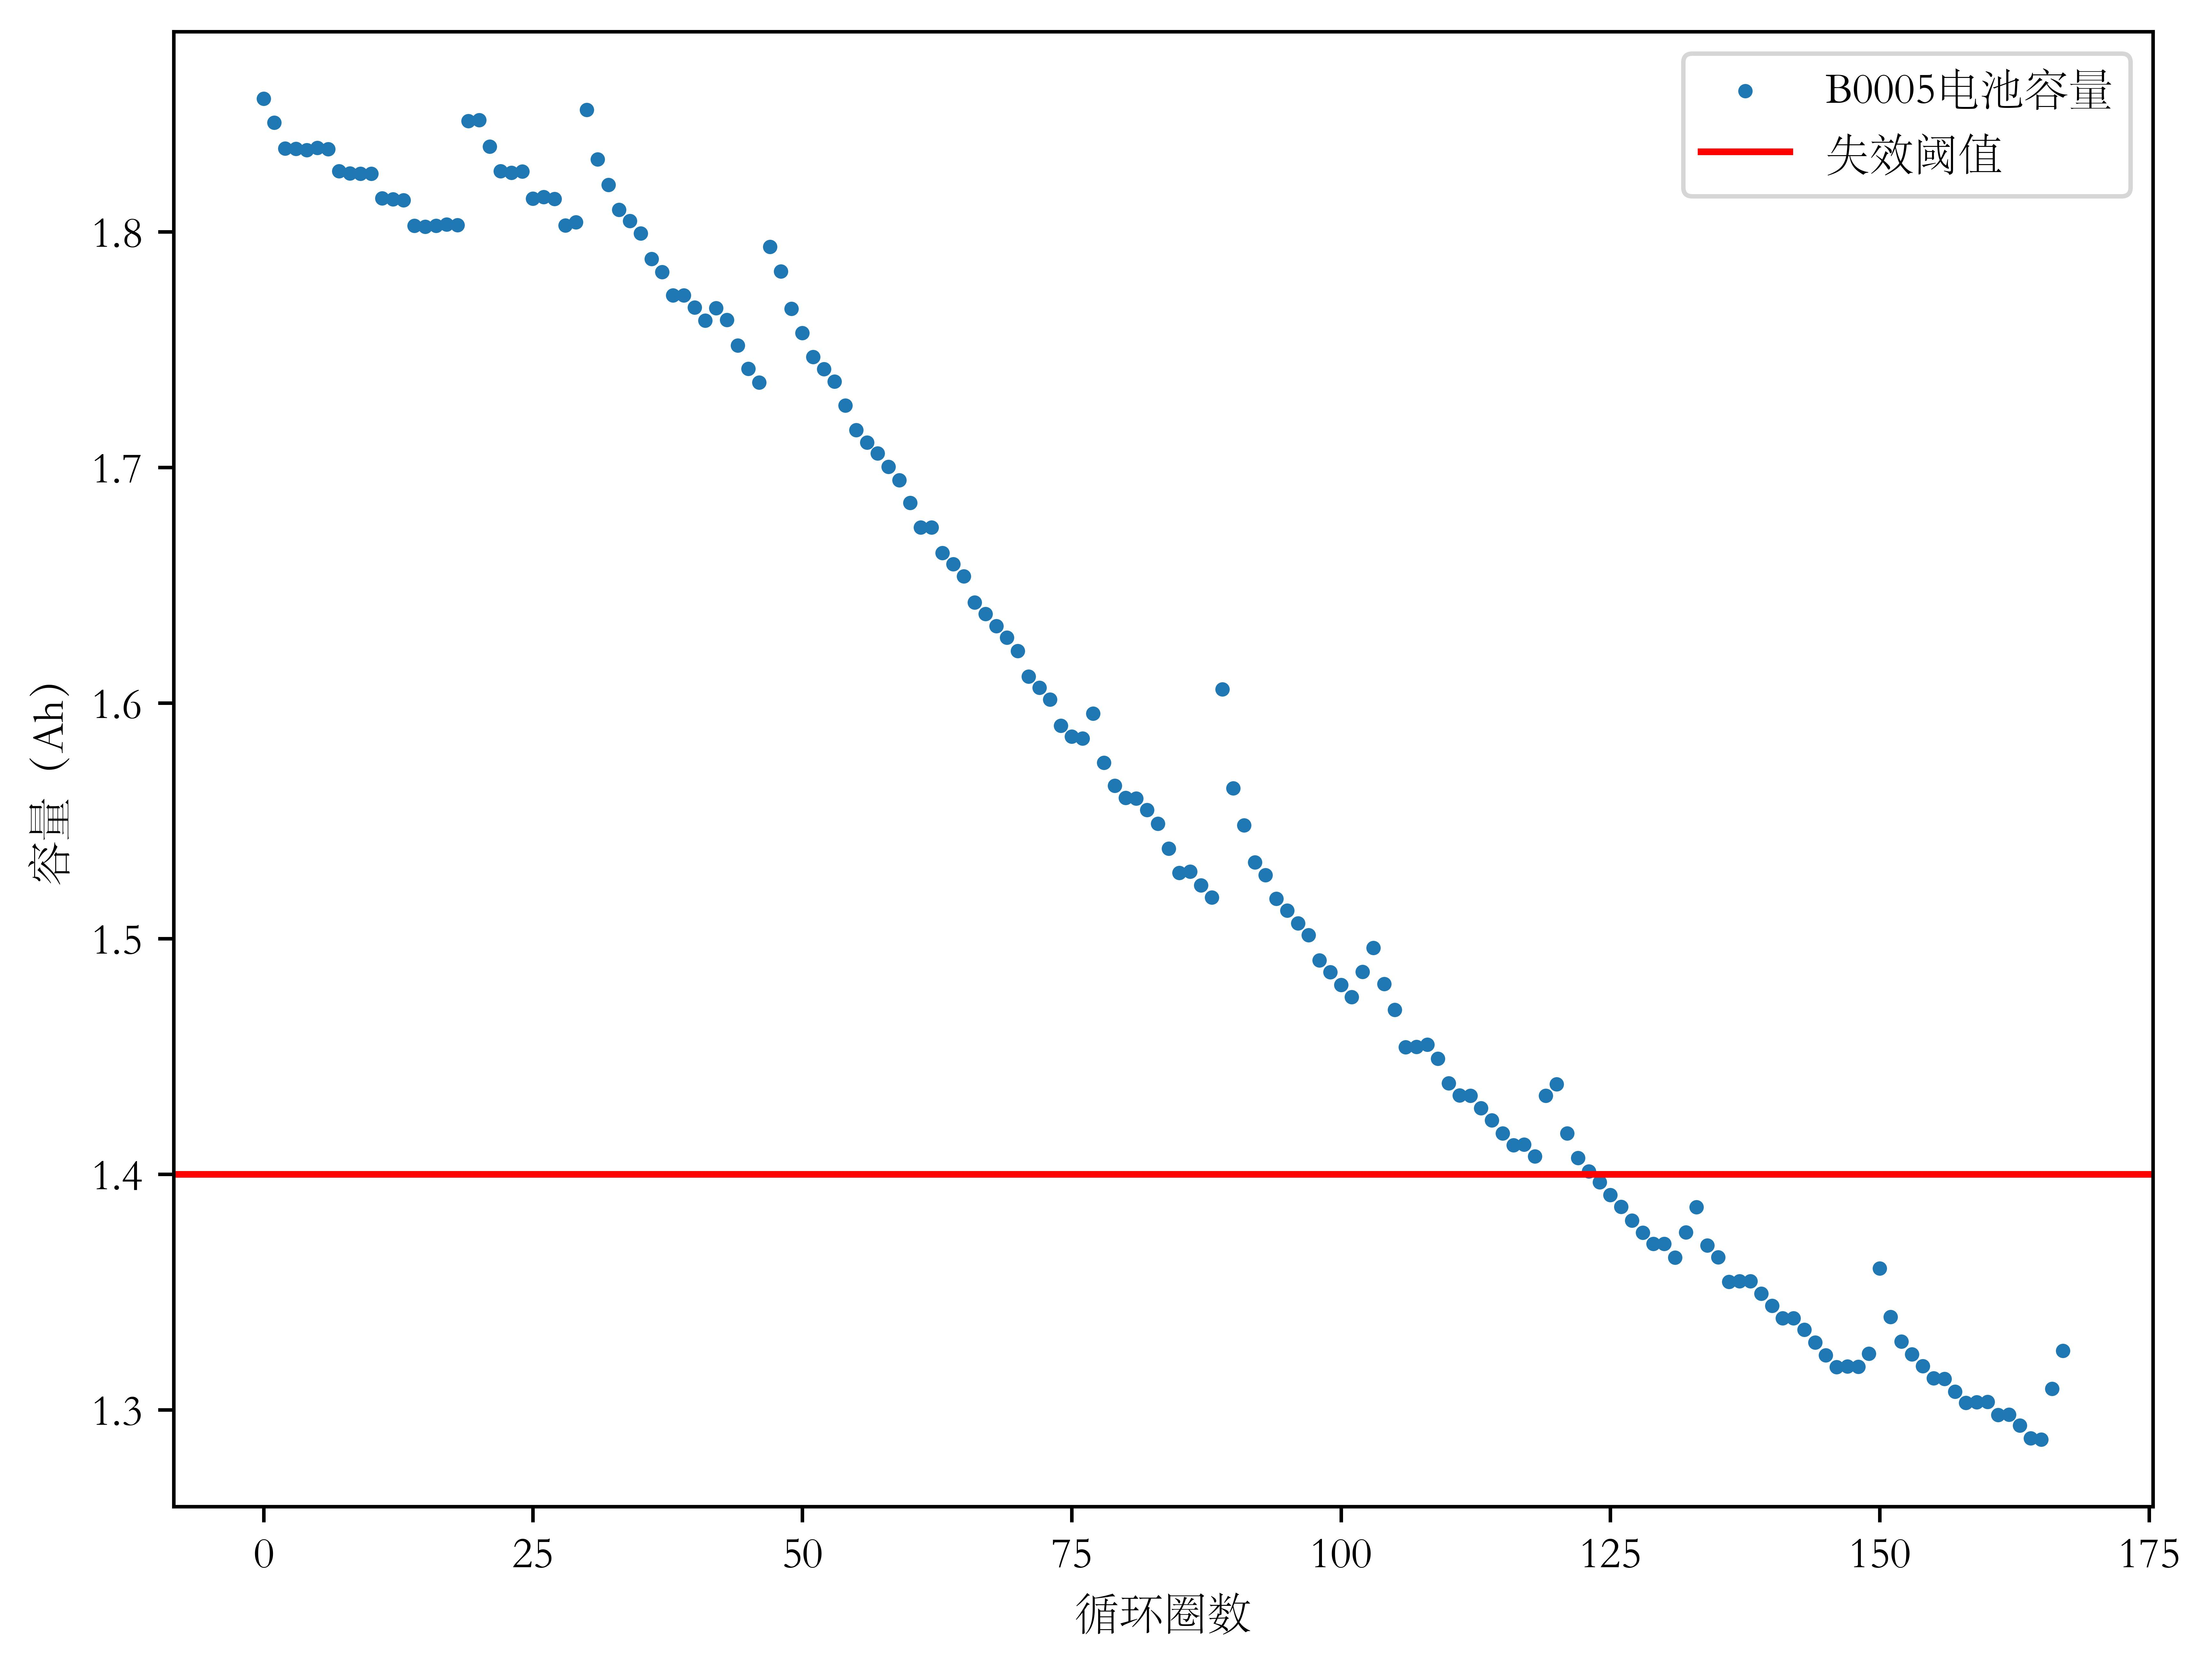
\includegraphics[scale=0.2]{figures/nasa_B0005_failure_threshold.jpg}
	% \end{figure}
	\begin{figure}[htbp]    % 常规操作\begin{figure}开头说明插入图片
		% 后面跟着的[htbp]是图片在文档中放置的位置,也称为浮动体的位置,关于这个我们后面的文章会聊聊,现在不管,照写就是了
		  \centering            % 前面说过,图片放置在中间
		  \subfloat[SOH]   % 第一张子图的下标(注意:注释要写在[]中括号内)
		  {\label{fig:subfig1}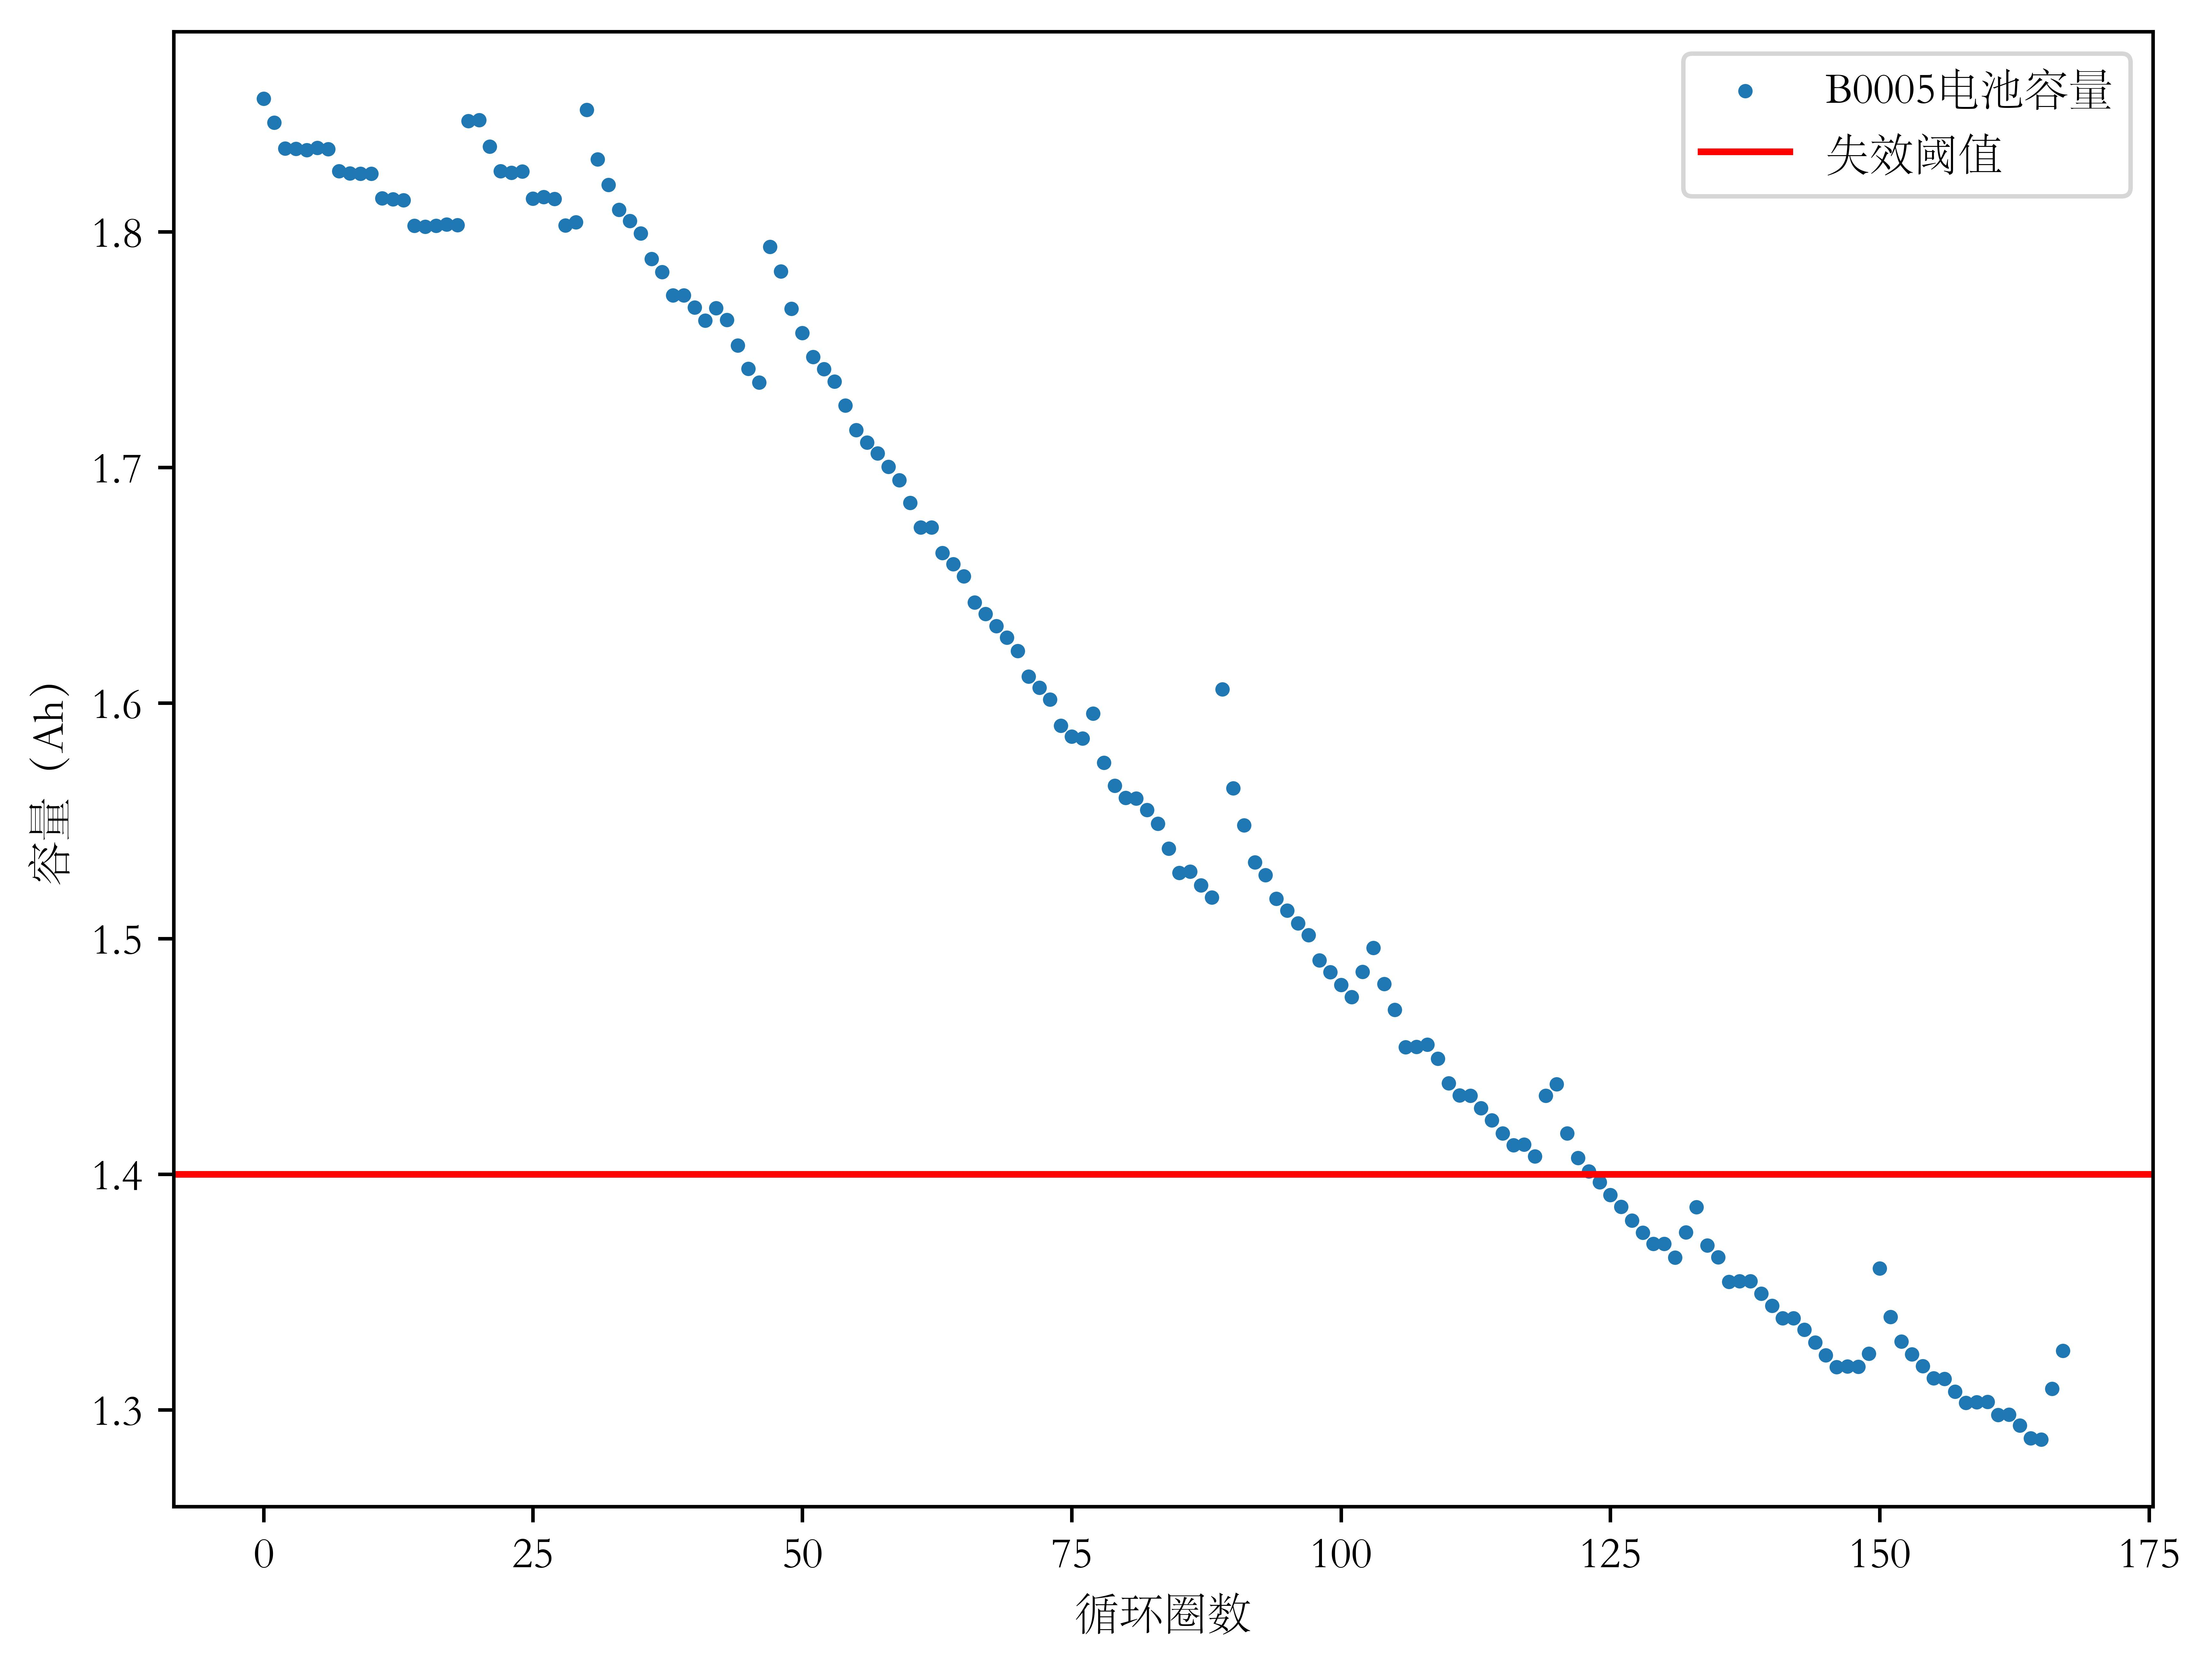
\includegraphics[width=0.25\textwidth]{figures/nasa_B0005_failure_threshold.jpg}}
		  \subfloat[RUL]
		  {\label{fig:subfig2}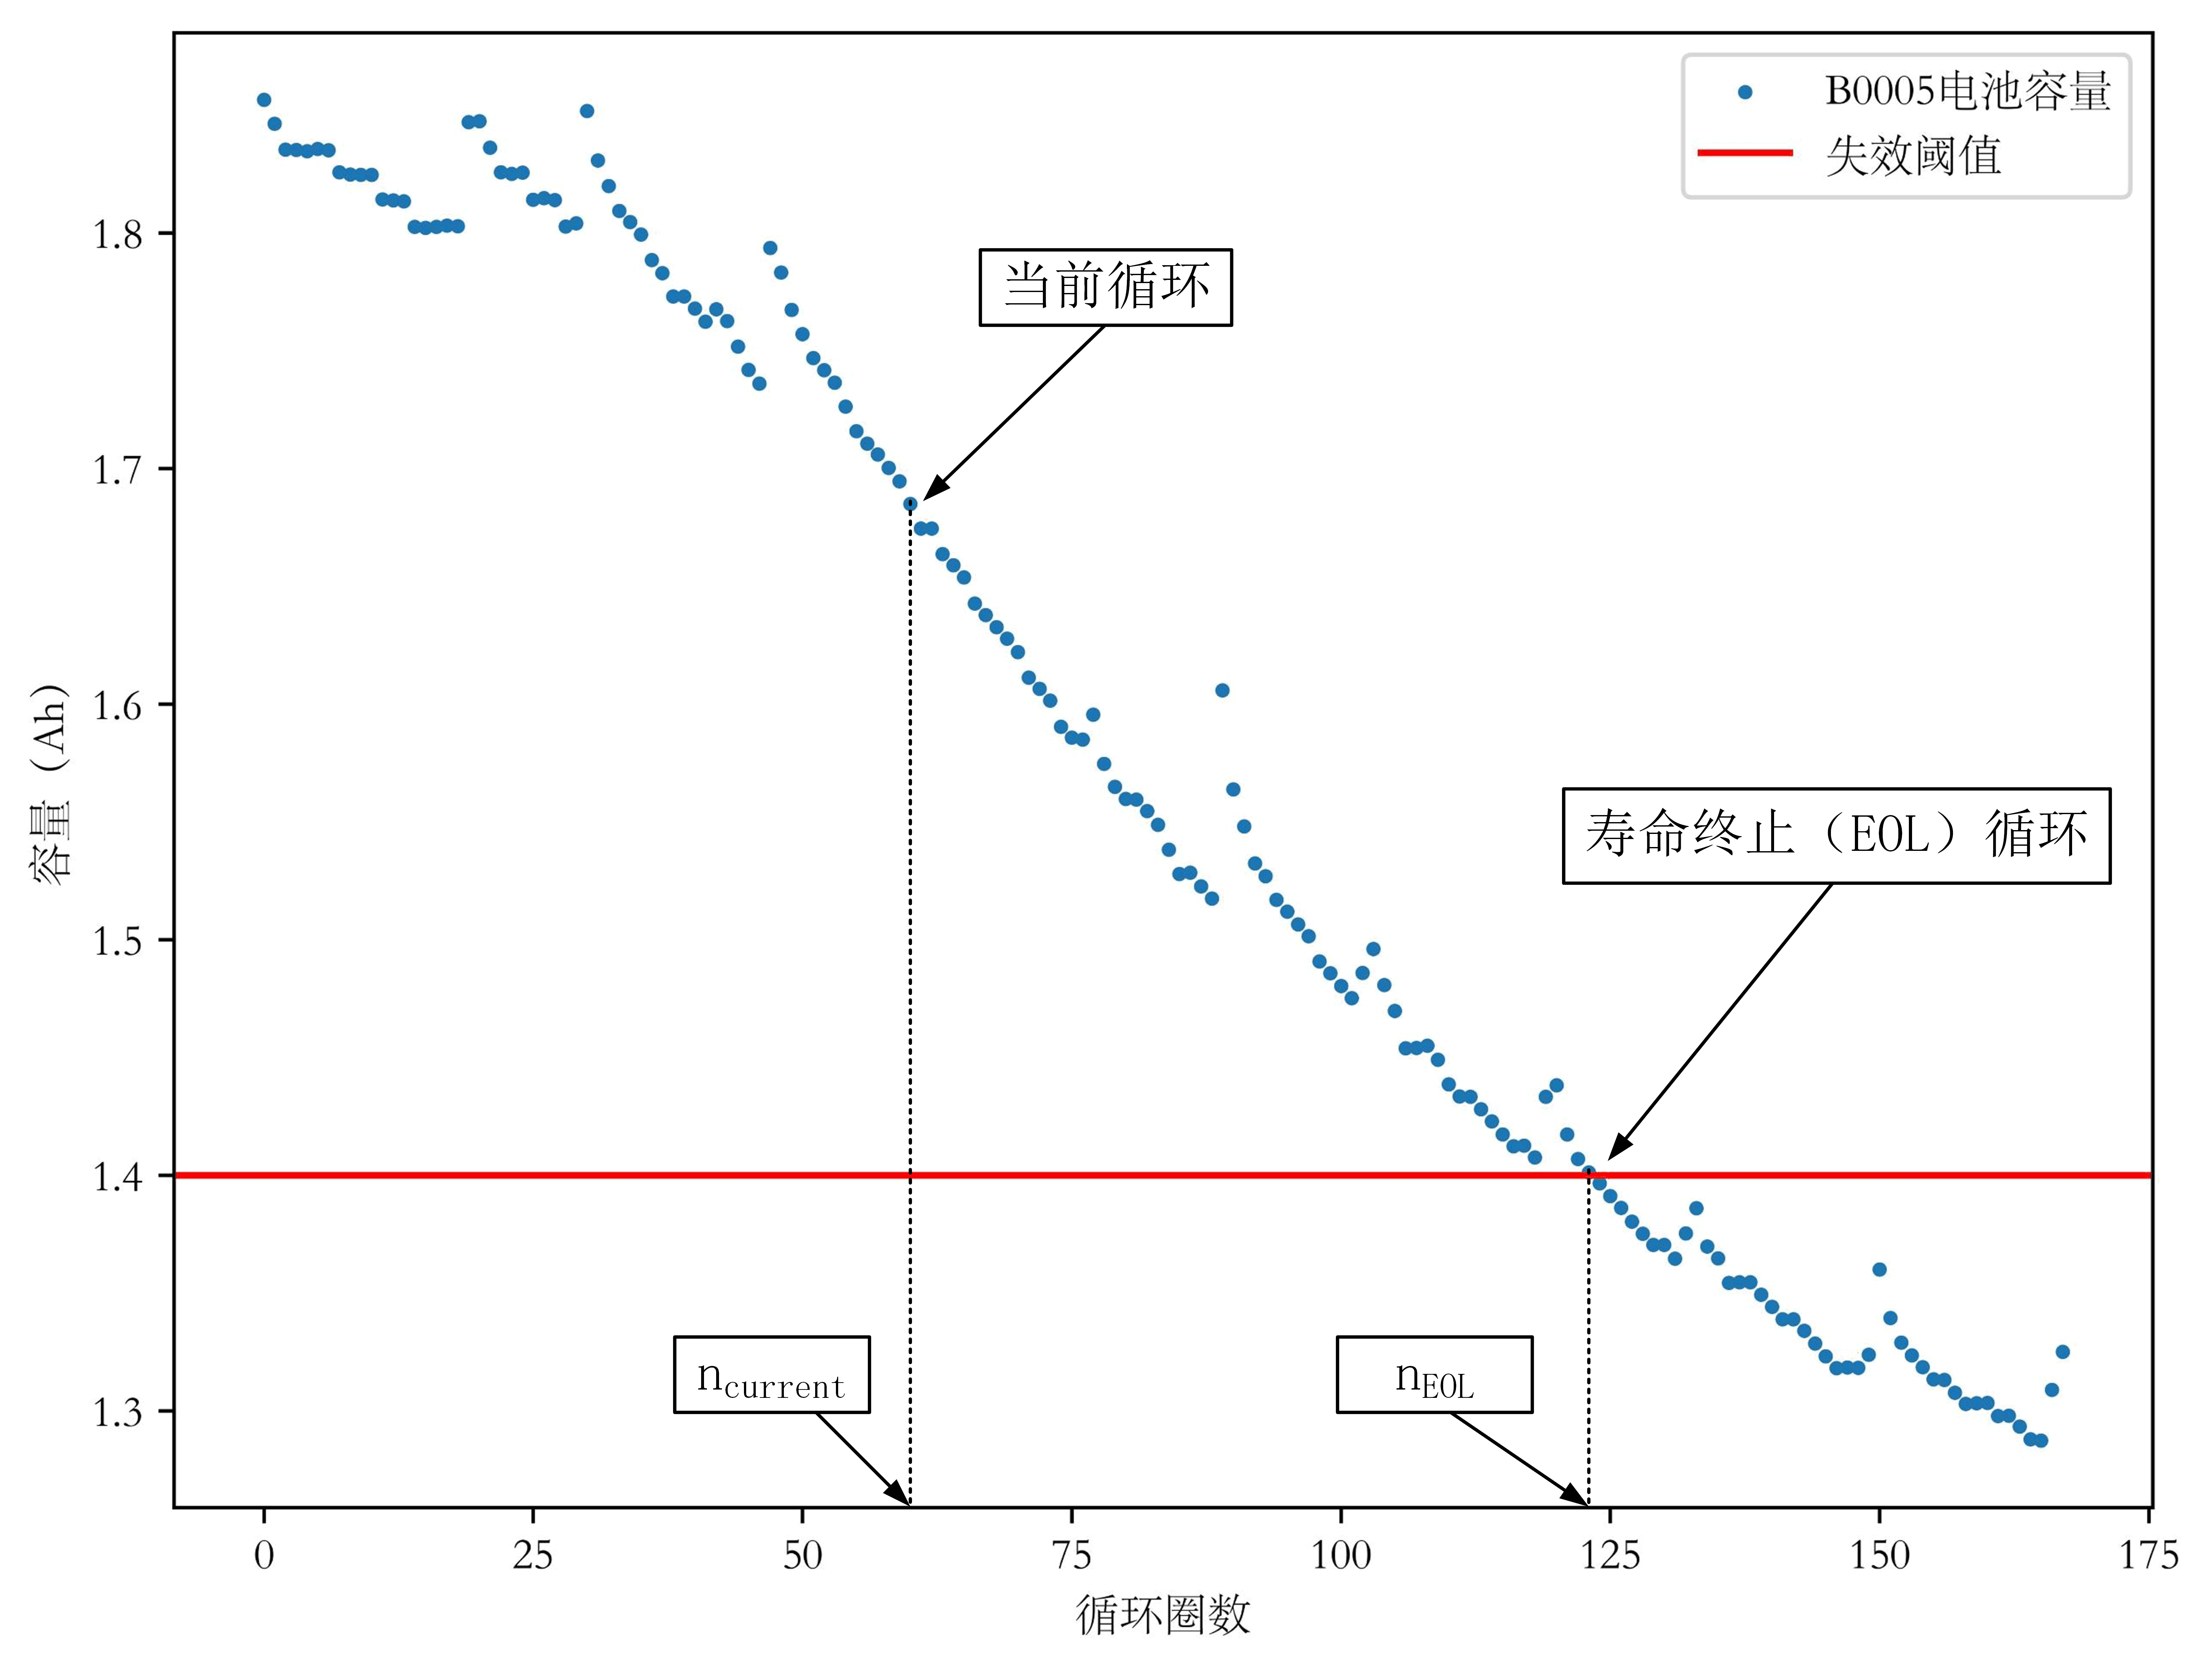
\includegraphics[width=0.25\textwidth]{figures/RUL.png}}
		  \subfloat[SOC]
		  {\label{fig:subfig3}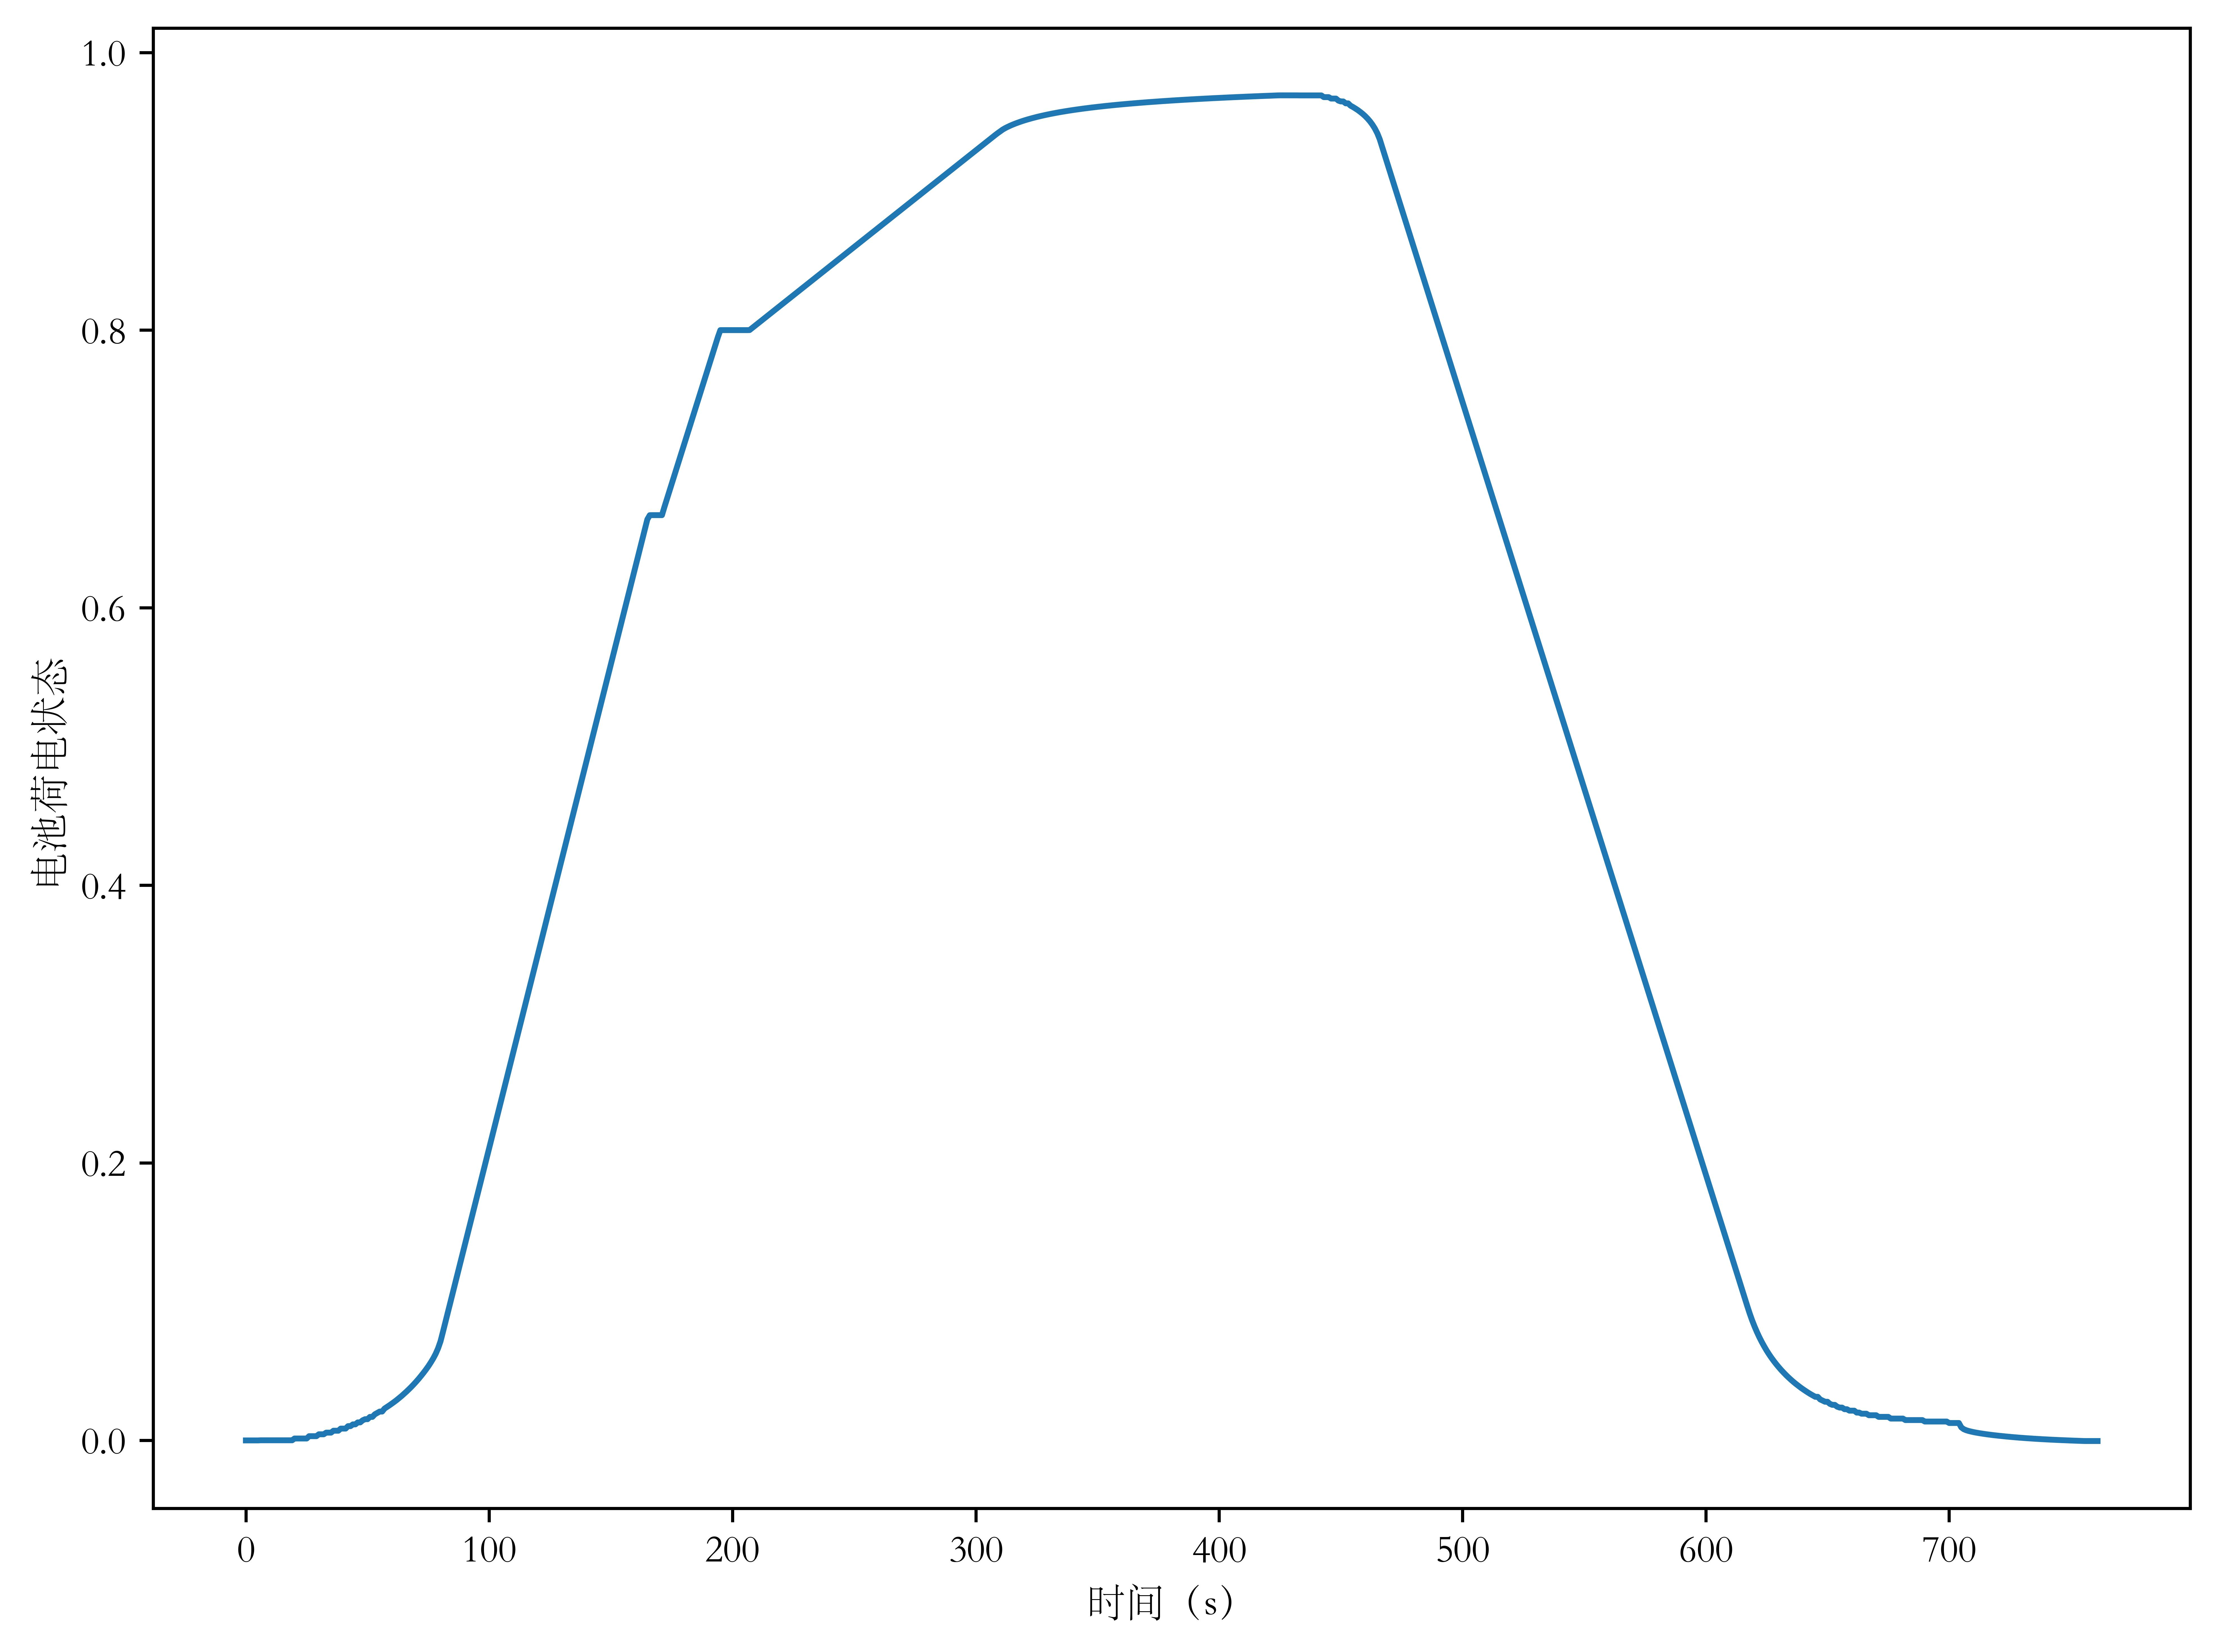
\includegraphics[width=0.25\textwidth]{figures/tri_b3c0_soc.jpg}}
		  % \caption{电池SOH、RUL和SOC示意图}    % 整个图片的说明,注释写在{}内
		\end{figure}
	\begin{description}
		\item[SOH]
		电池健康状态,使用电池放电容量表征,描述电池性能退化状态,$SOH = \frac{Q_{max}}{Q_{nominal}}$
		\item[RUL]
		电池剩余寿命,描述电池从当前循环到寿命终止(EOL)循环的过程,$RUL = n_{EOL} - n_{current}$
		\item[SOC]
		电池荷电状态,和SOH有相同的形式,描述电池电荷量,$SOC = \frac{Q_{remain}}{Q_{max}}$
	\end{description}
\end{frame}

\section{建模和实验}

\subsection{基于电池容量历史退化数据的SOH估计}

\begin{frame}
	\begin{figure}[htbp]
		\centering
			{\label{fig:subfig1}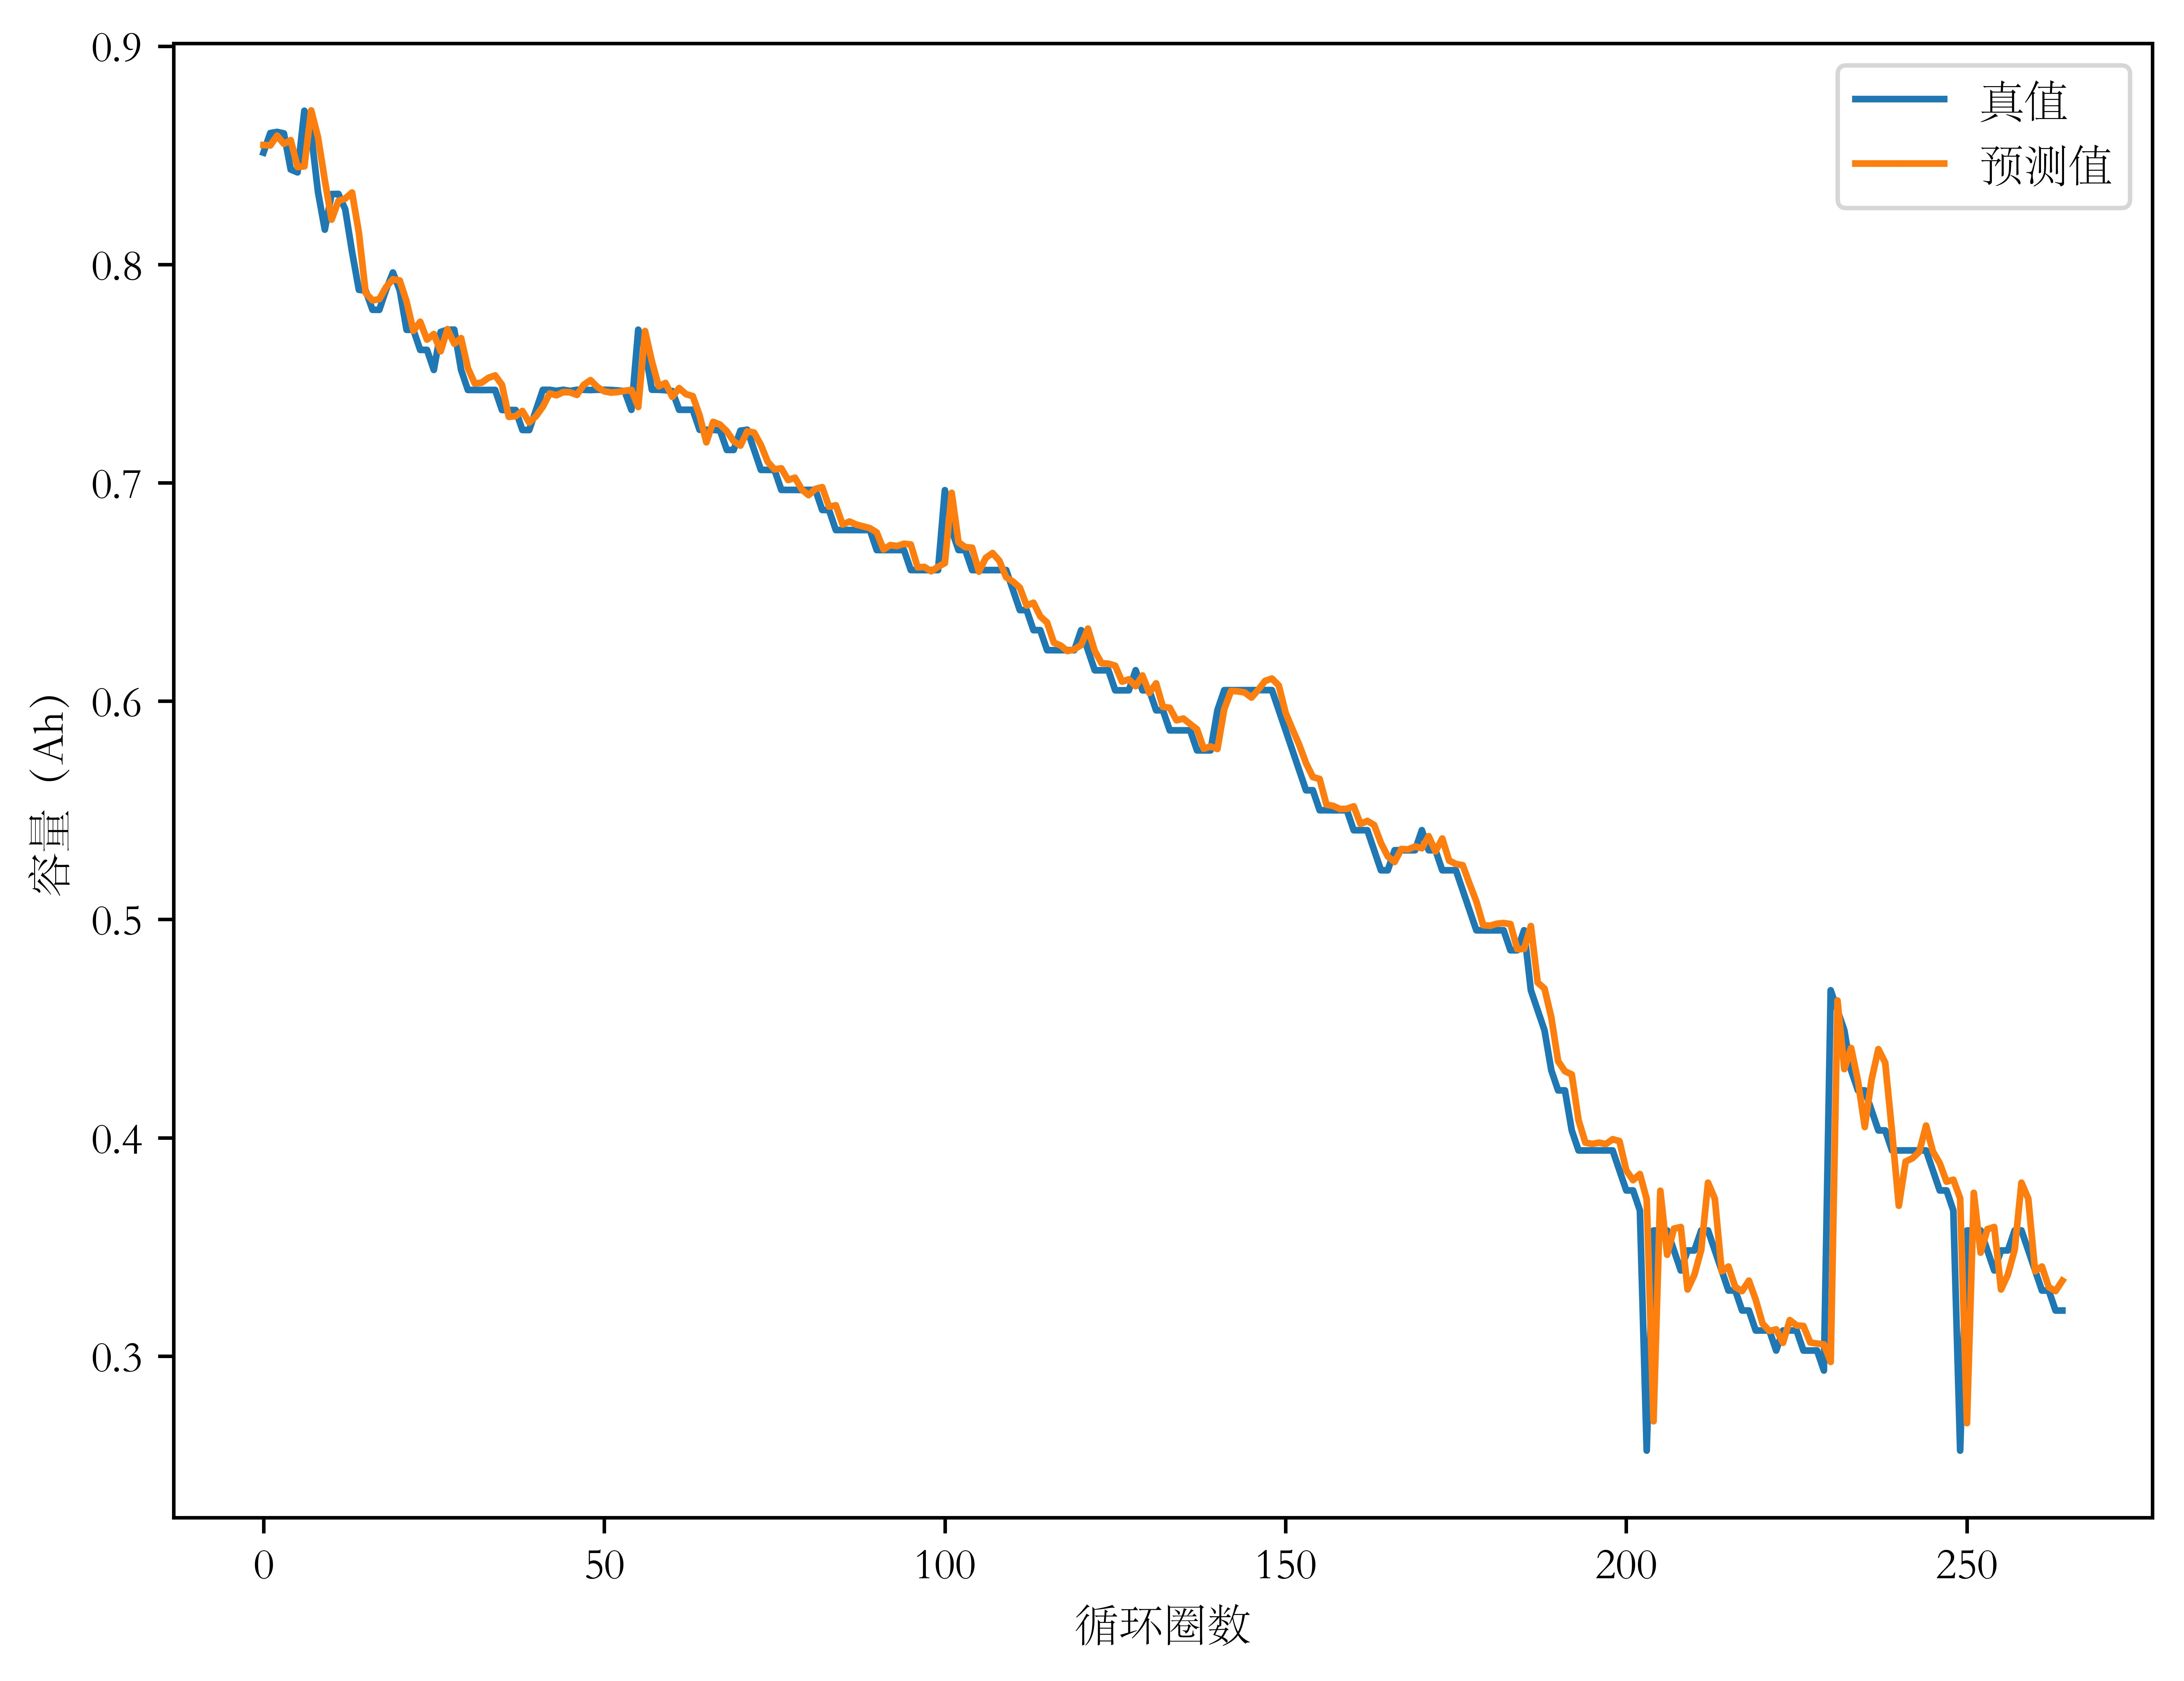
\includegraphics[width=0.15\textwidth]{figures/soh_cap/calce_CS2_35_ar.jpg}}
			{\label{fig:subfig2}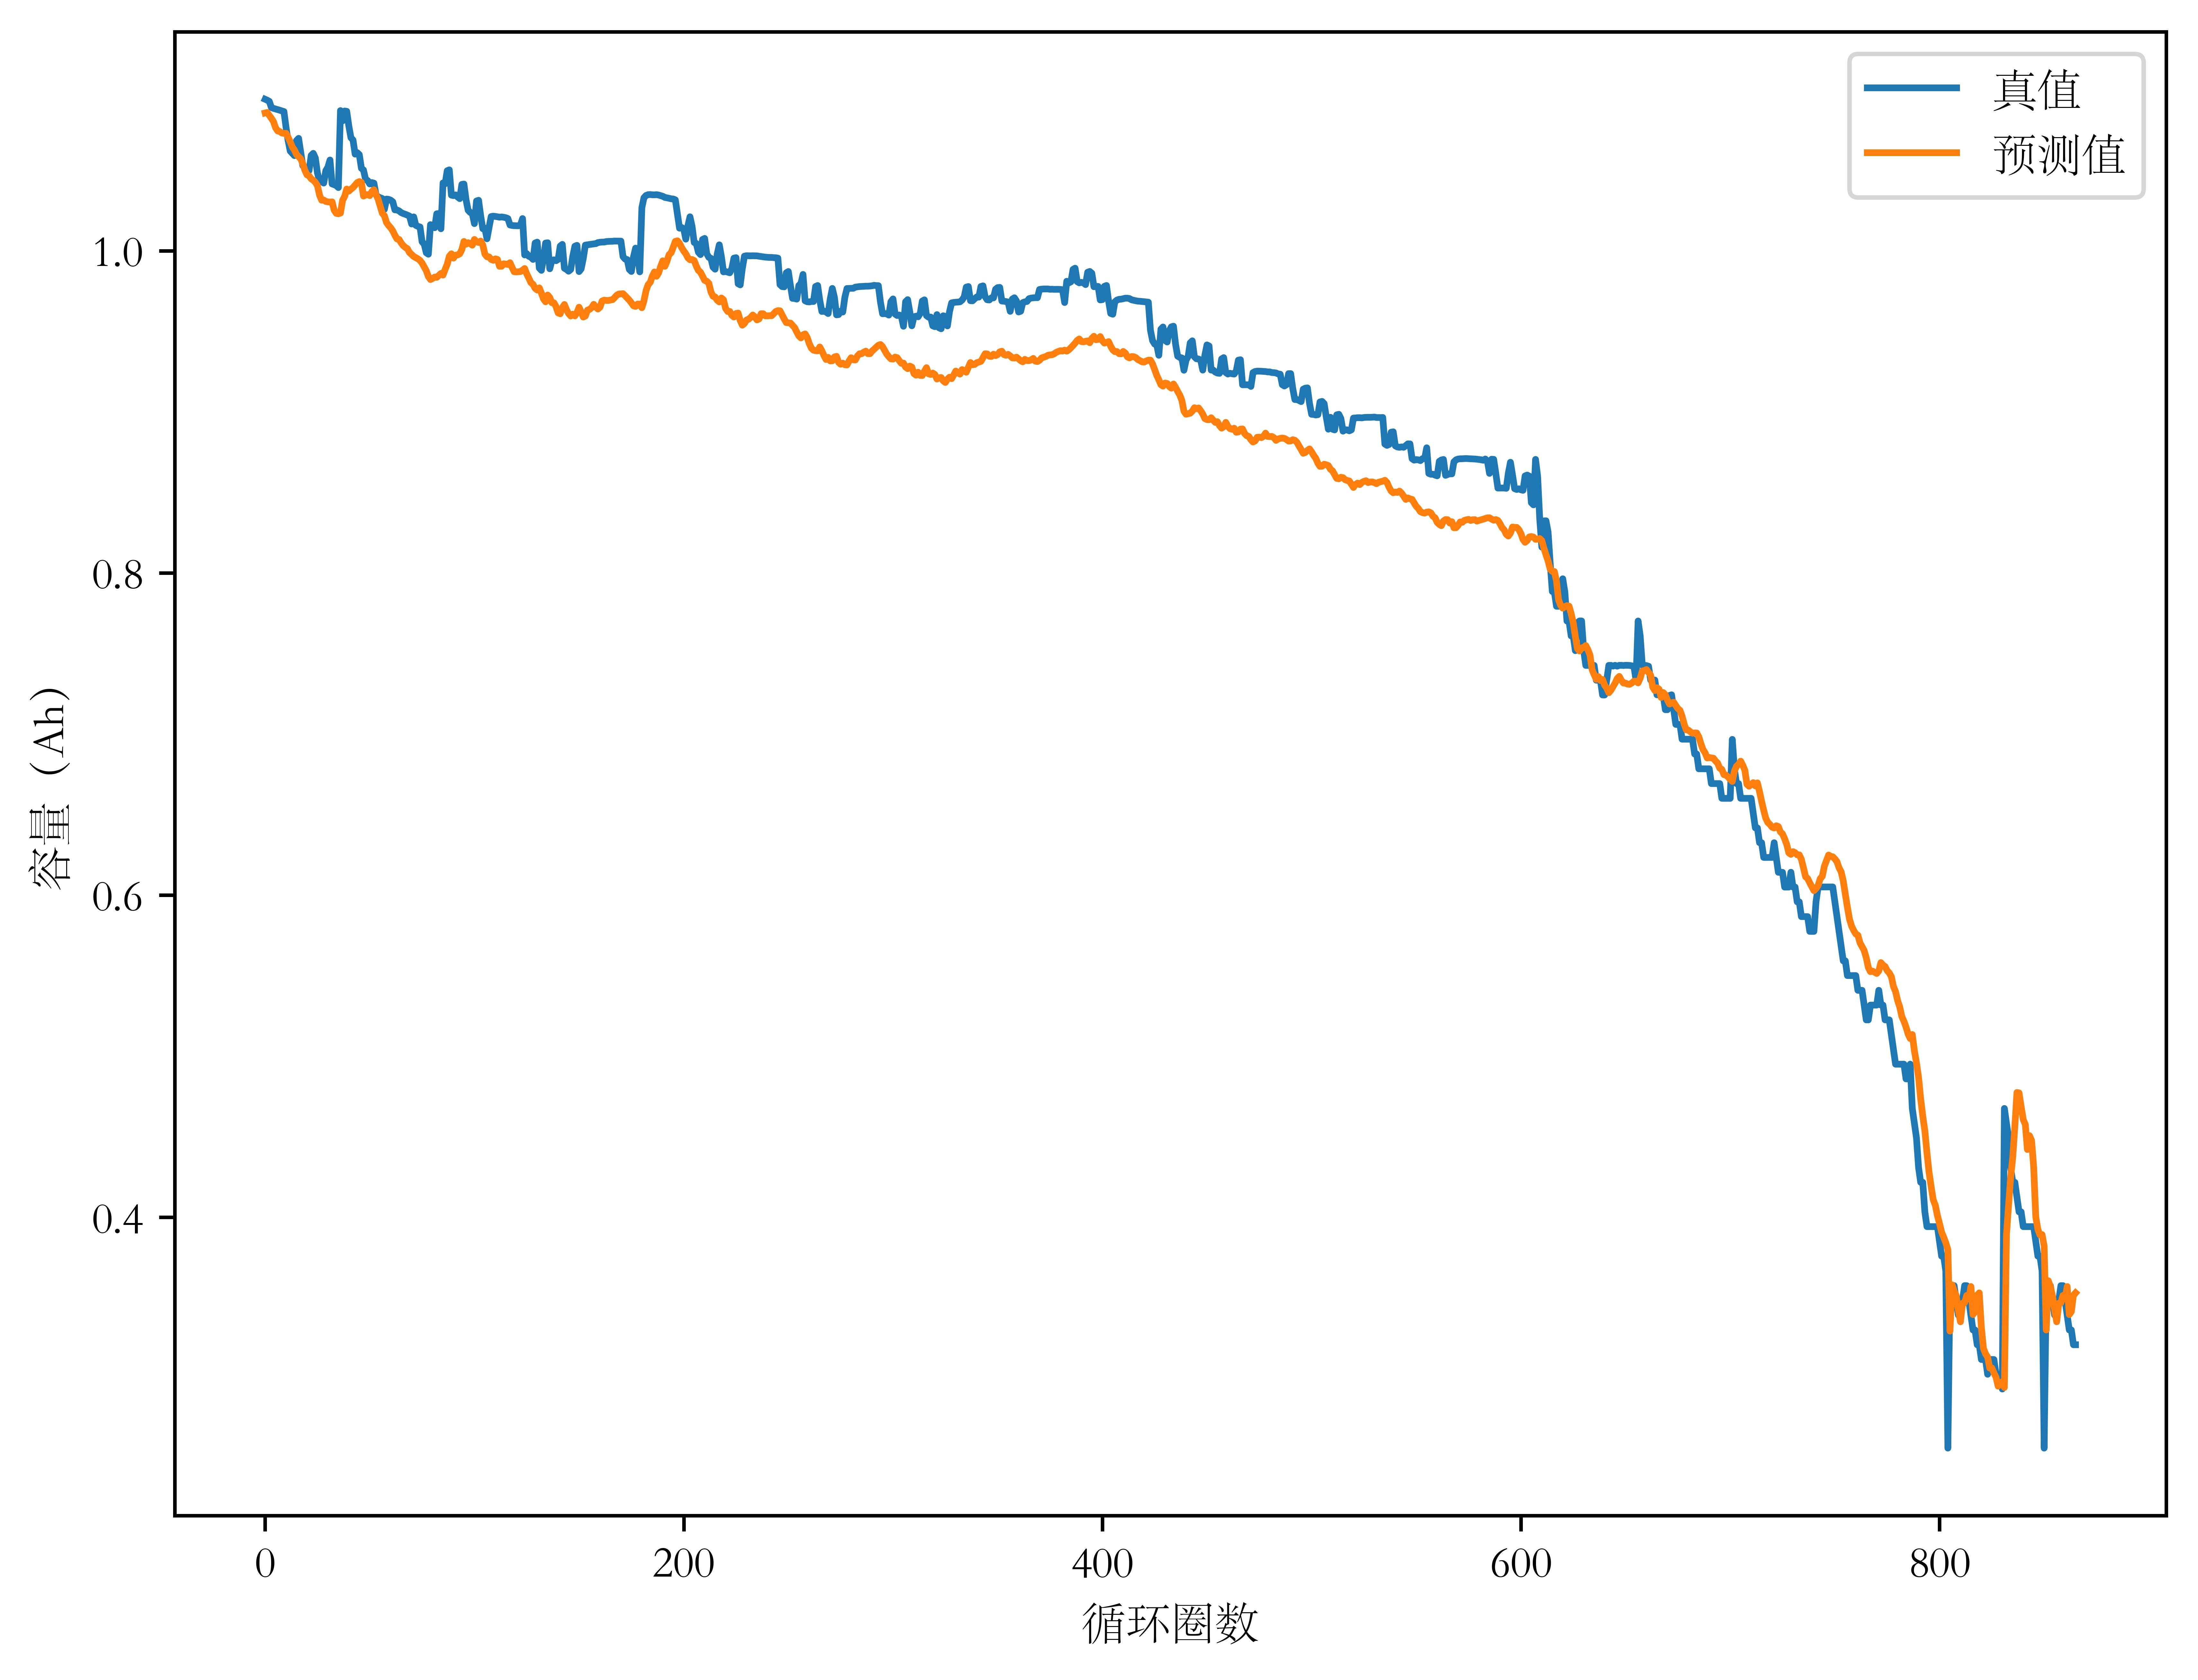
\includegraphics[width=0.15\textwidth]{figures/soh_cap/calce_CS2_35_svr.jpg}}
			{\label{fig:subfig3}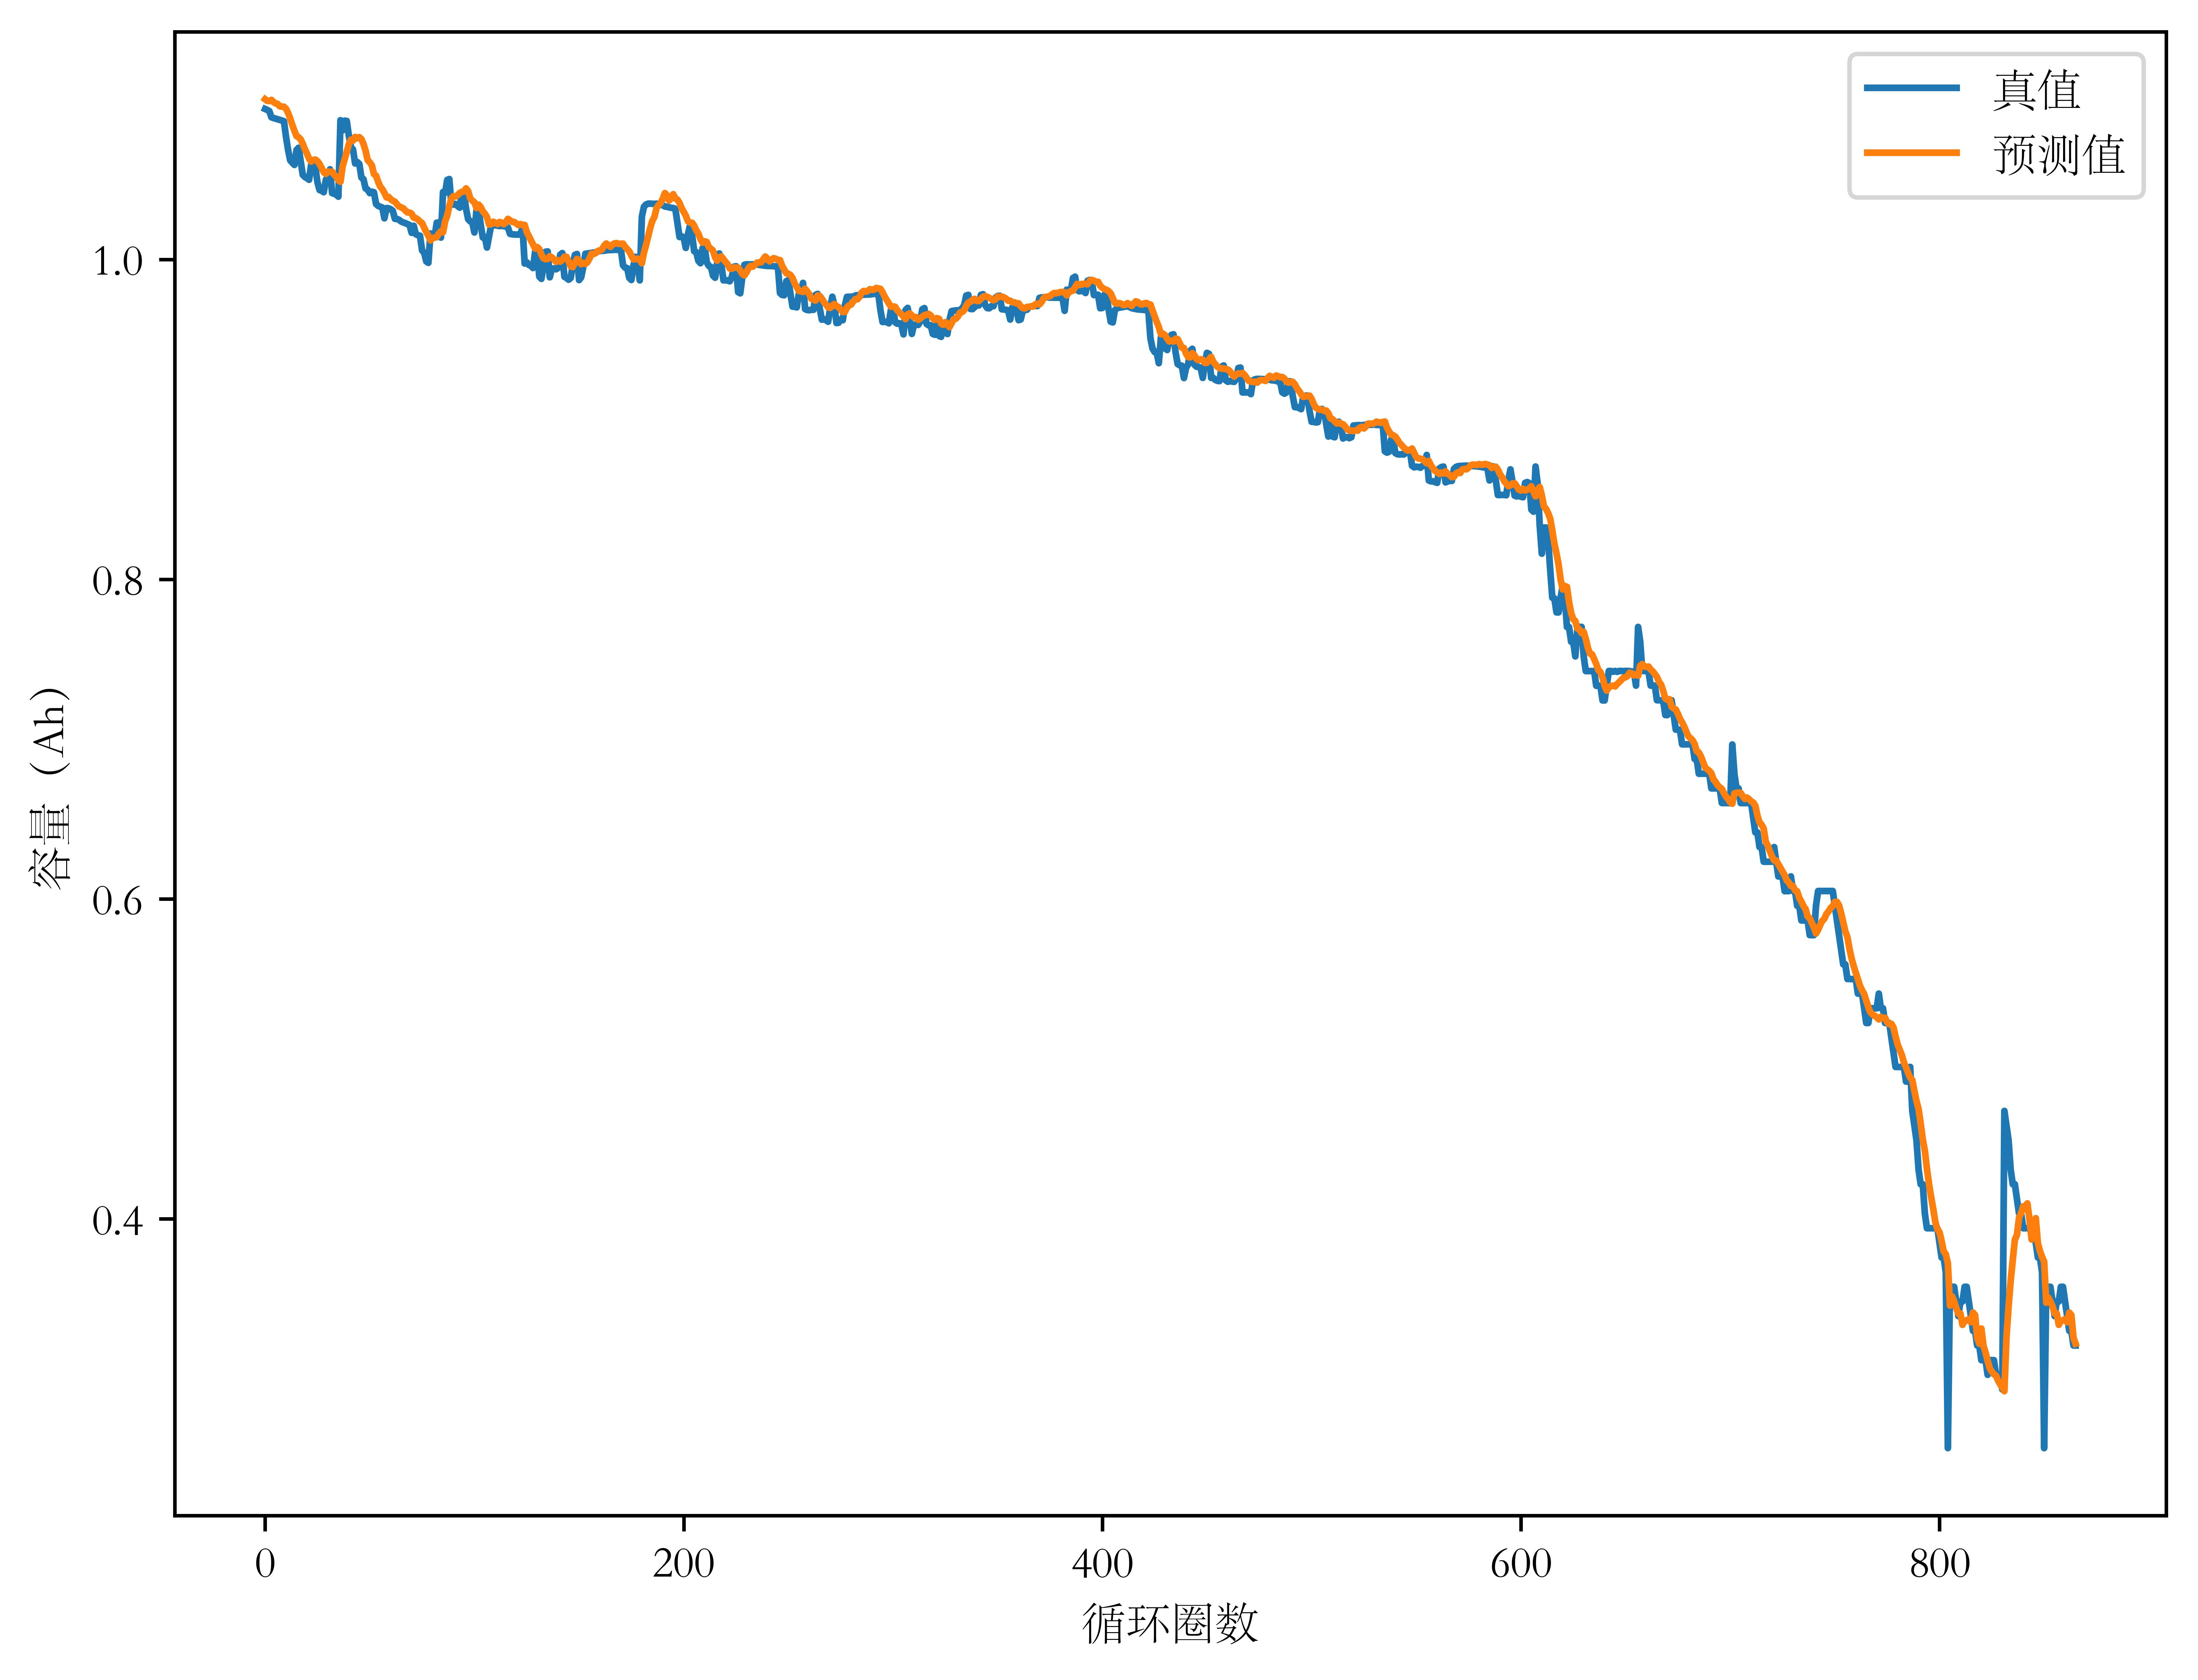
\includegraphics[width=0.15\textwidth]{figures/soh_cap/calce_CS2_35_mlp.jpg}}
			{\label{fig:subfig4}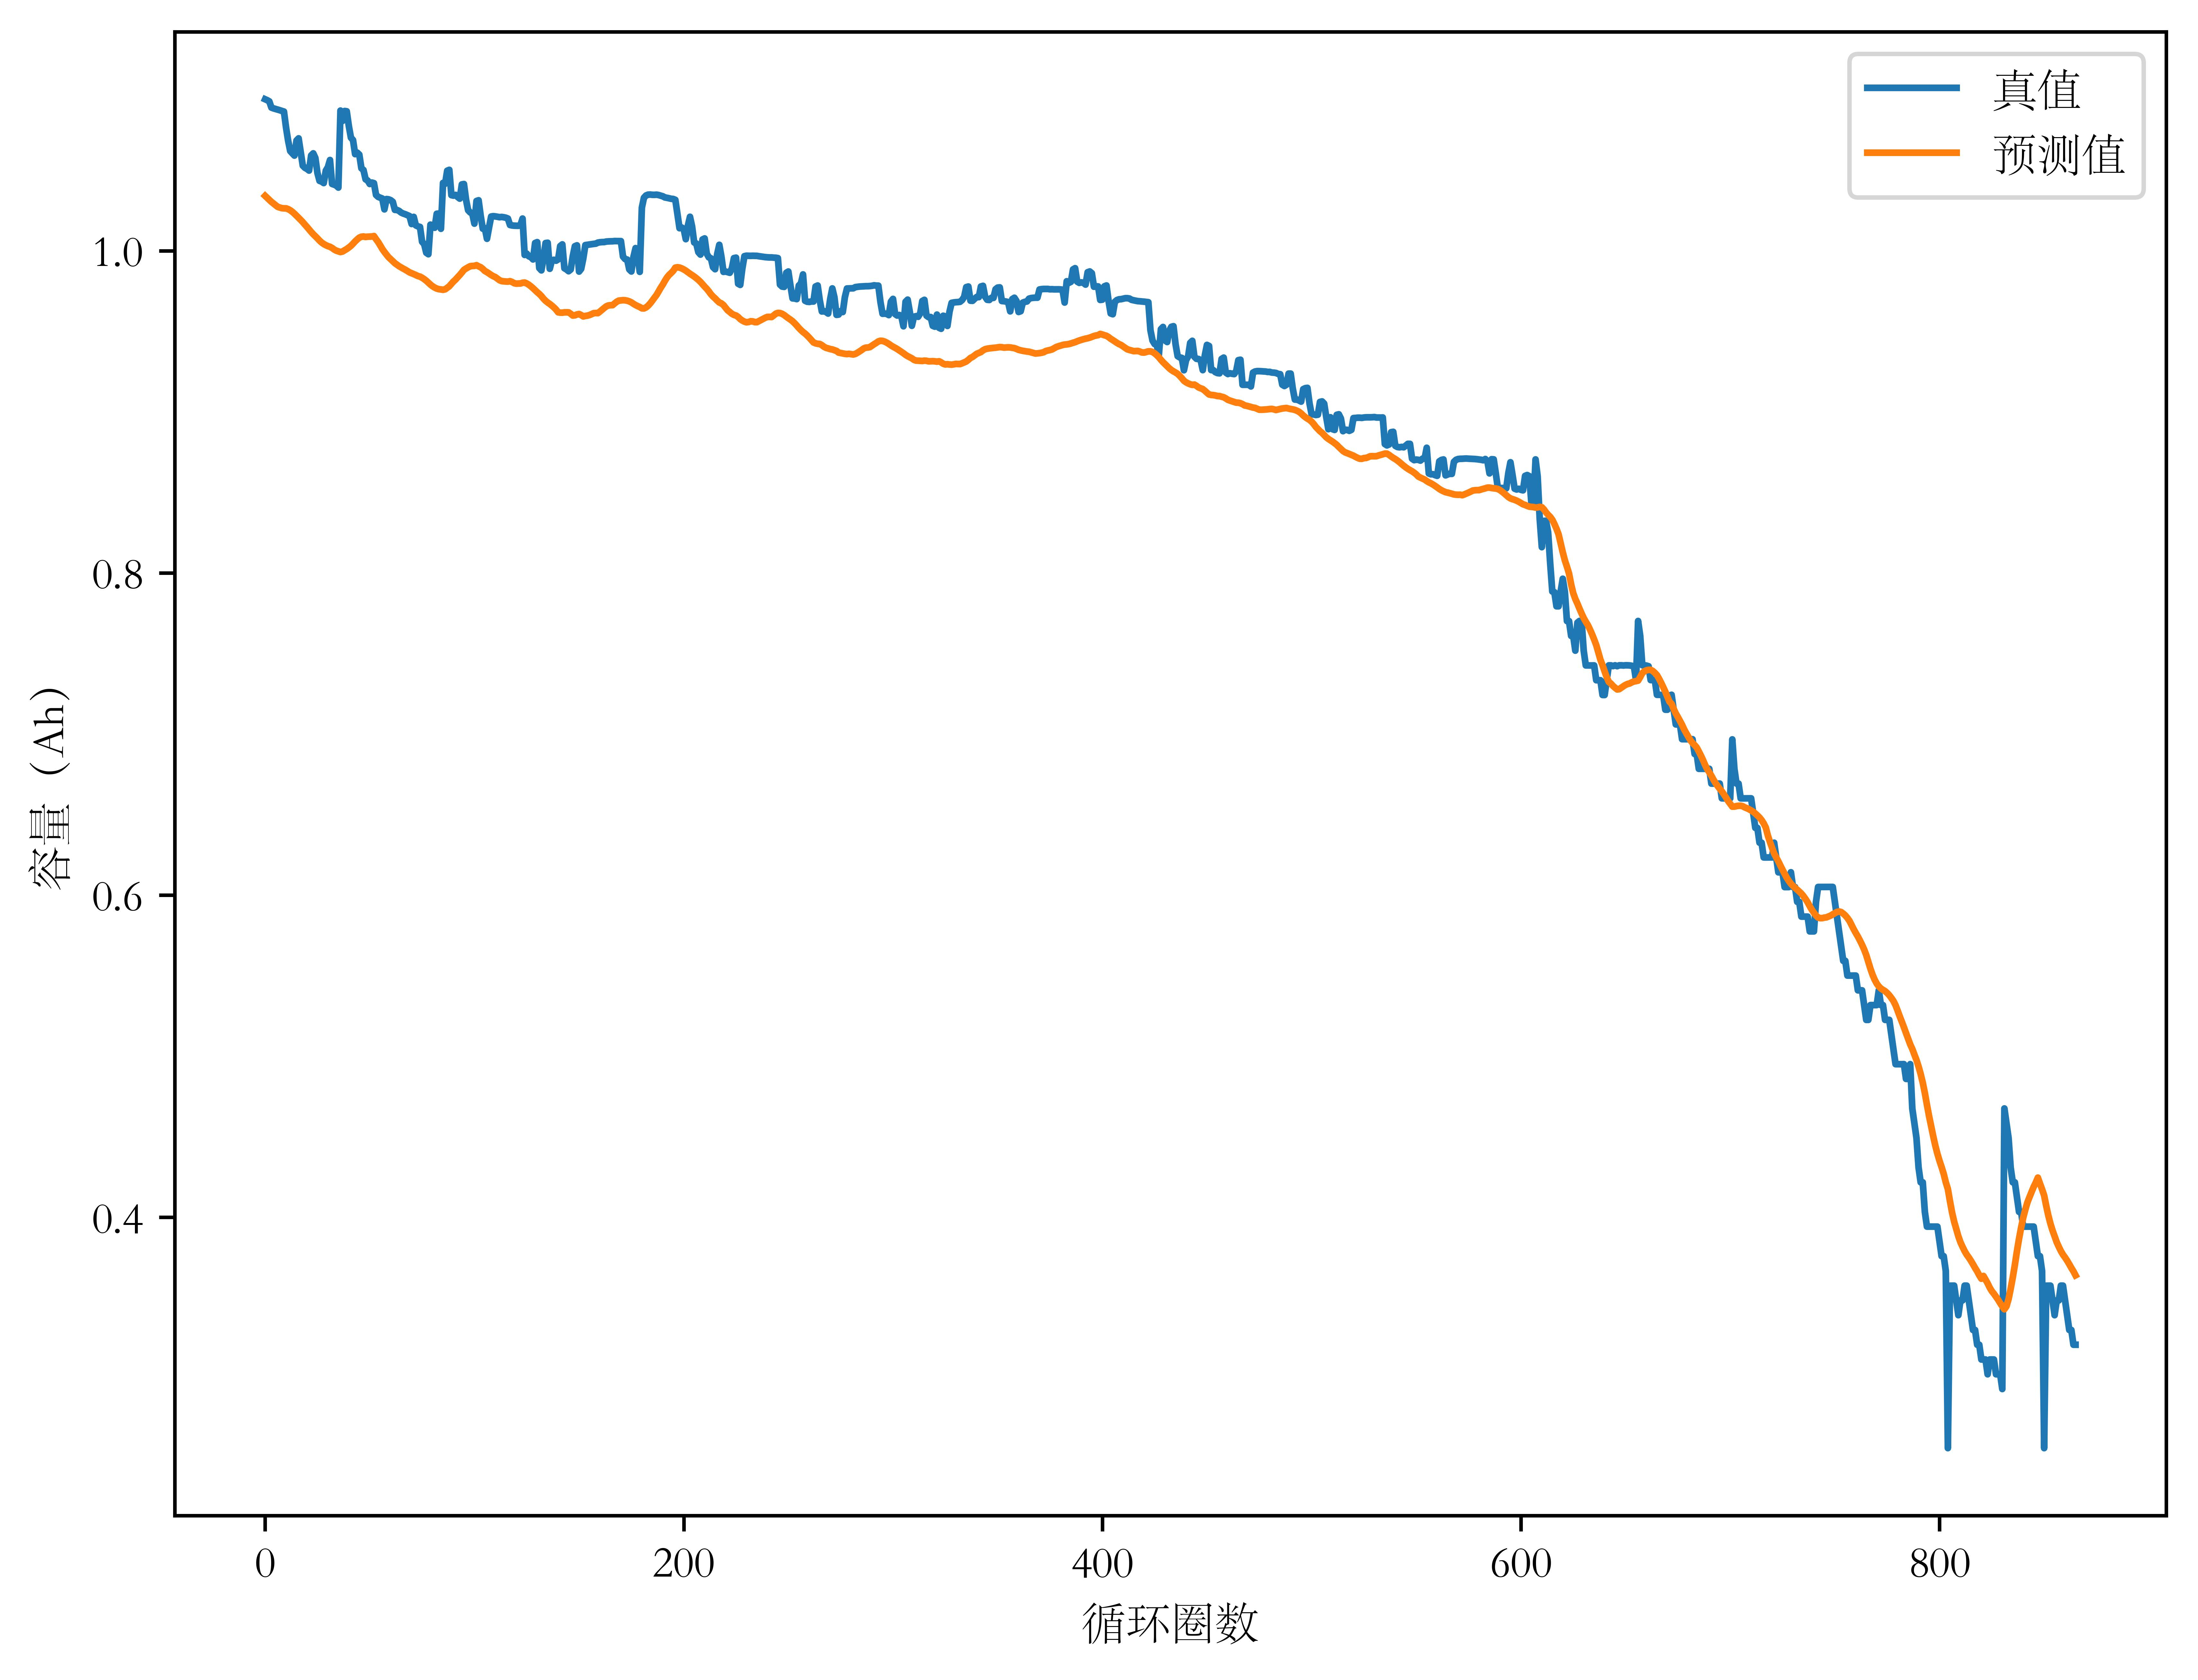
\includegraphics[width=0.15\textwidth]{figures/soh_cap/calce_CS2_35_lstm.jpg}}
			{\label{fig:subfig5}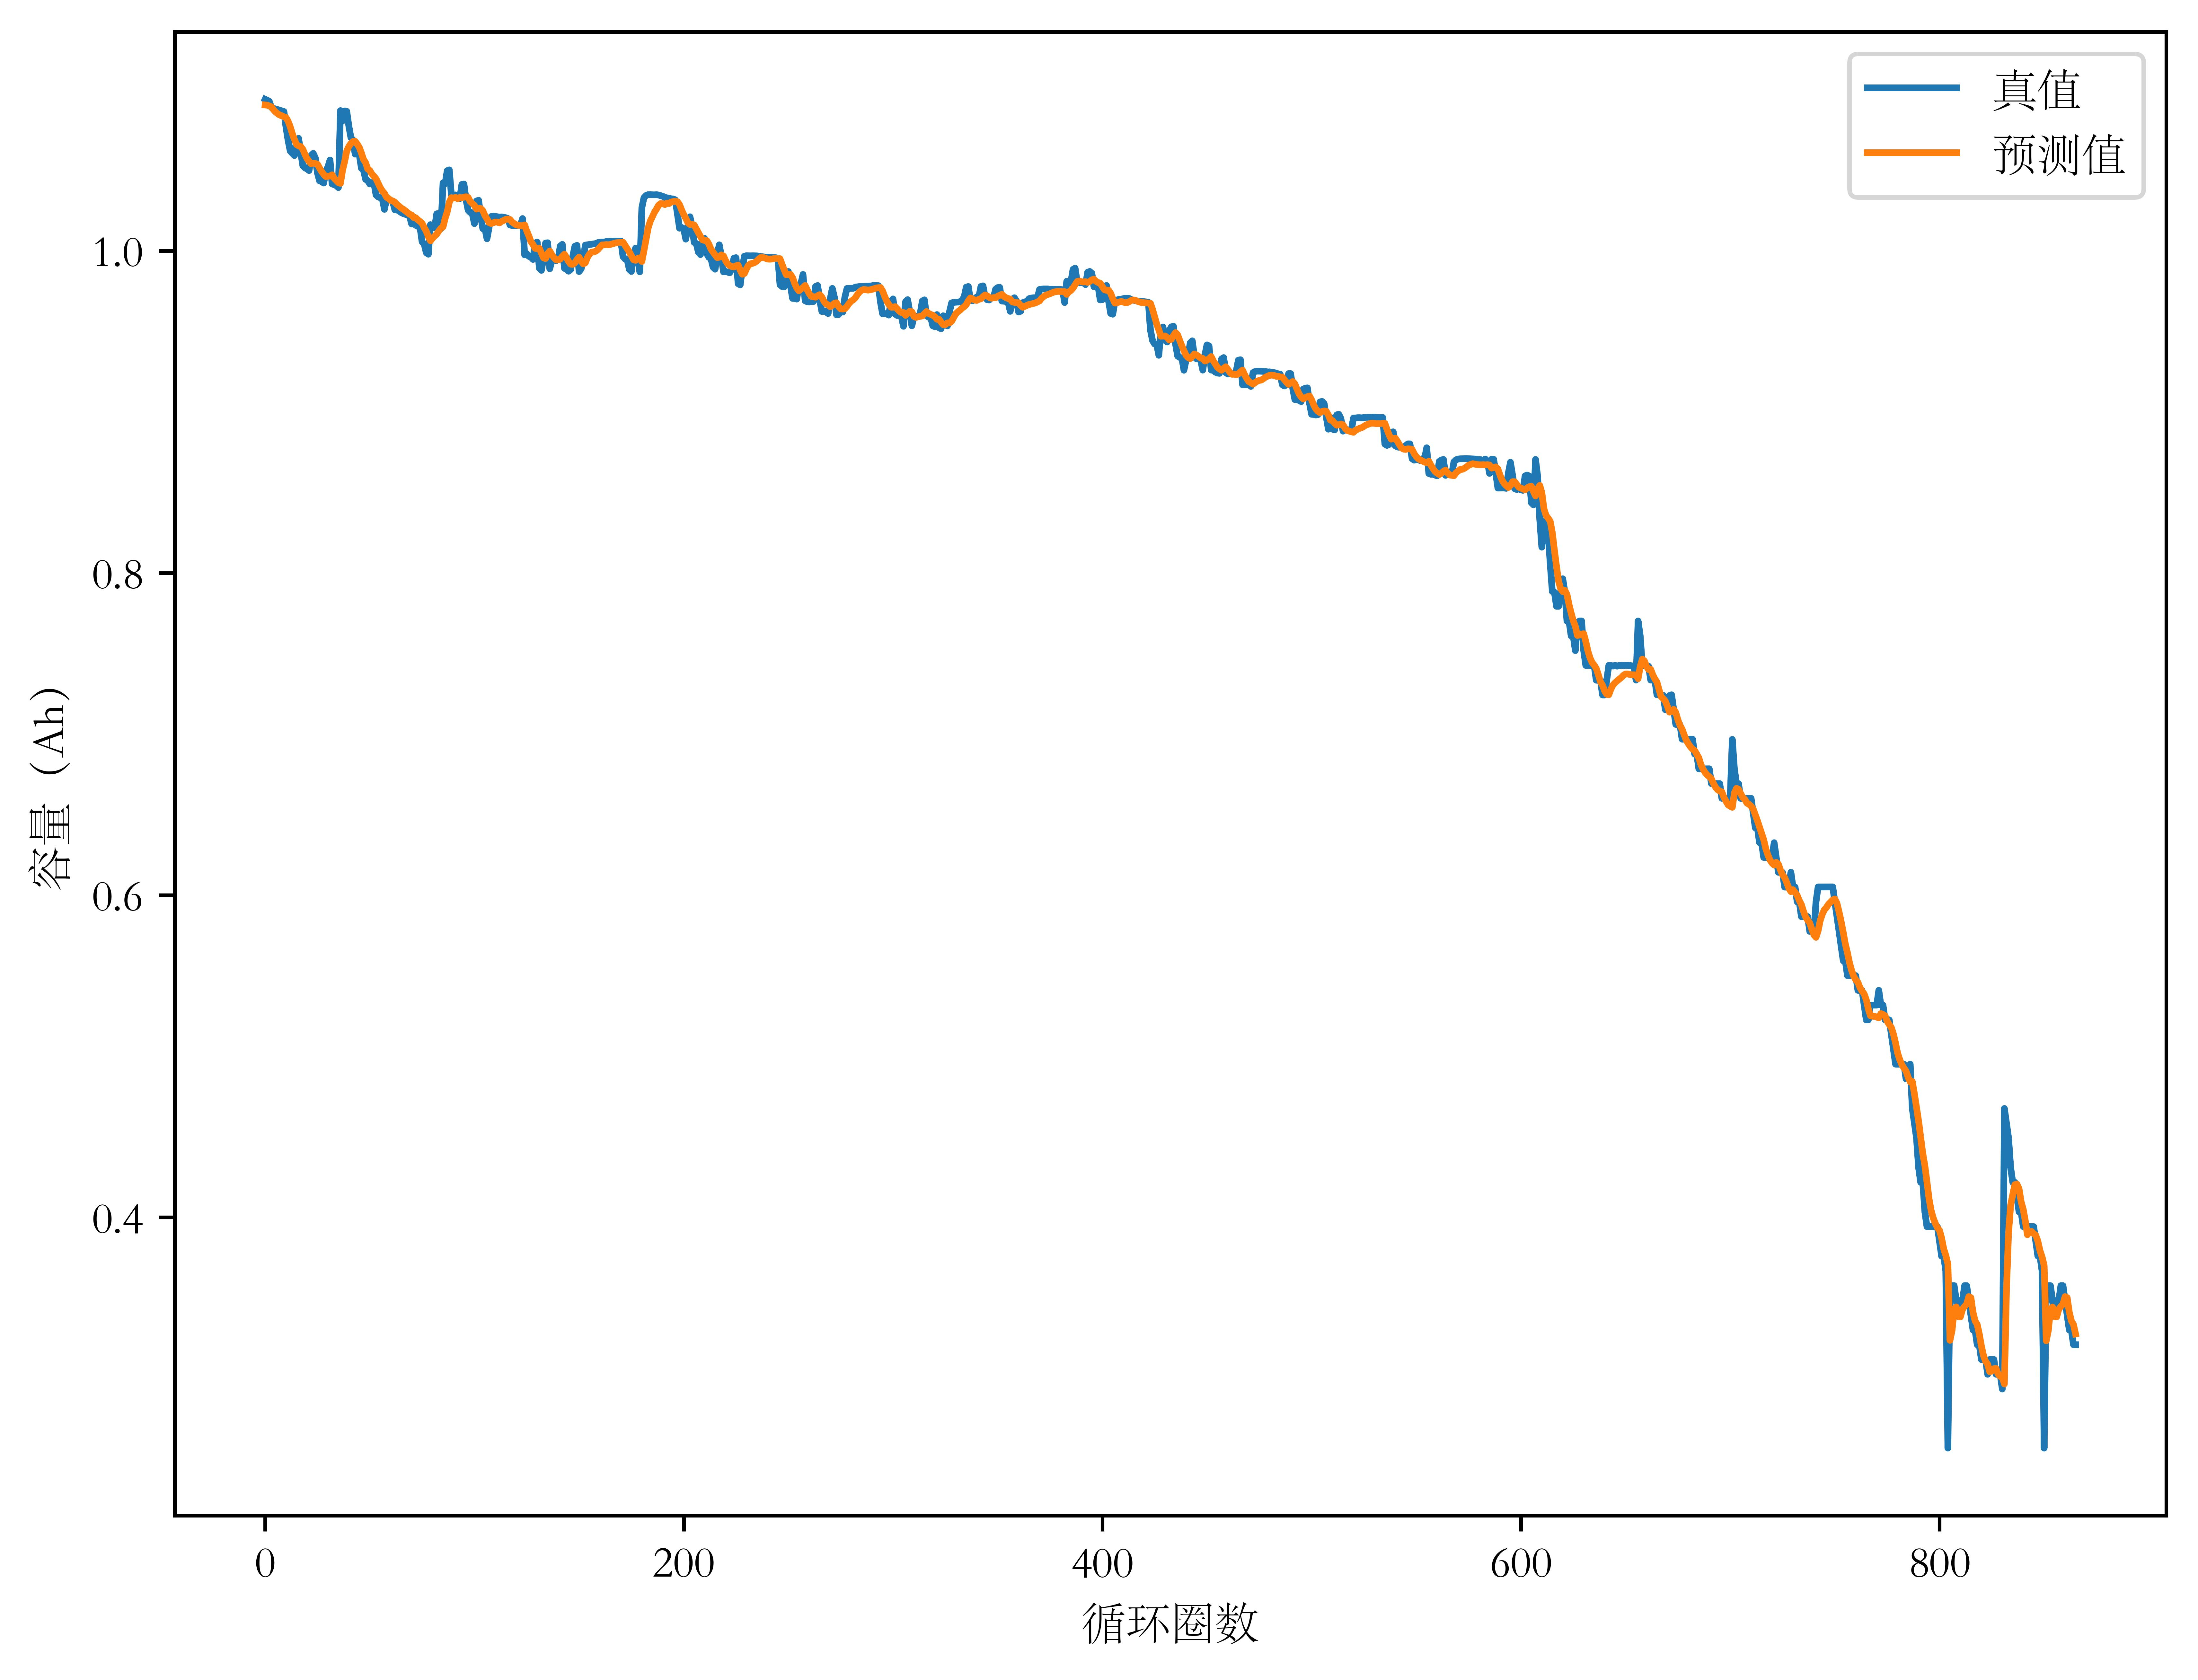
\includegraphics[width=0.15\textwidth]{figures/soh_cap/calce_CS2_35_cnn.jpg}}
	\end{figure}
	\begin{figure}[htbp]
		\centering
			{\label{fig:subfig1}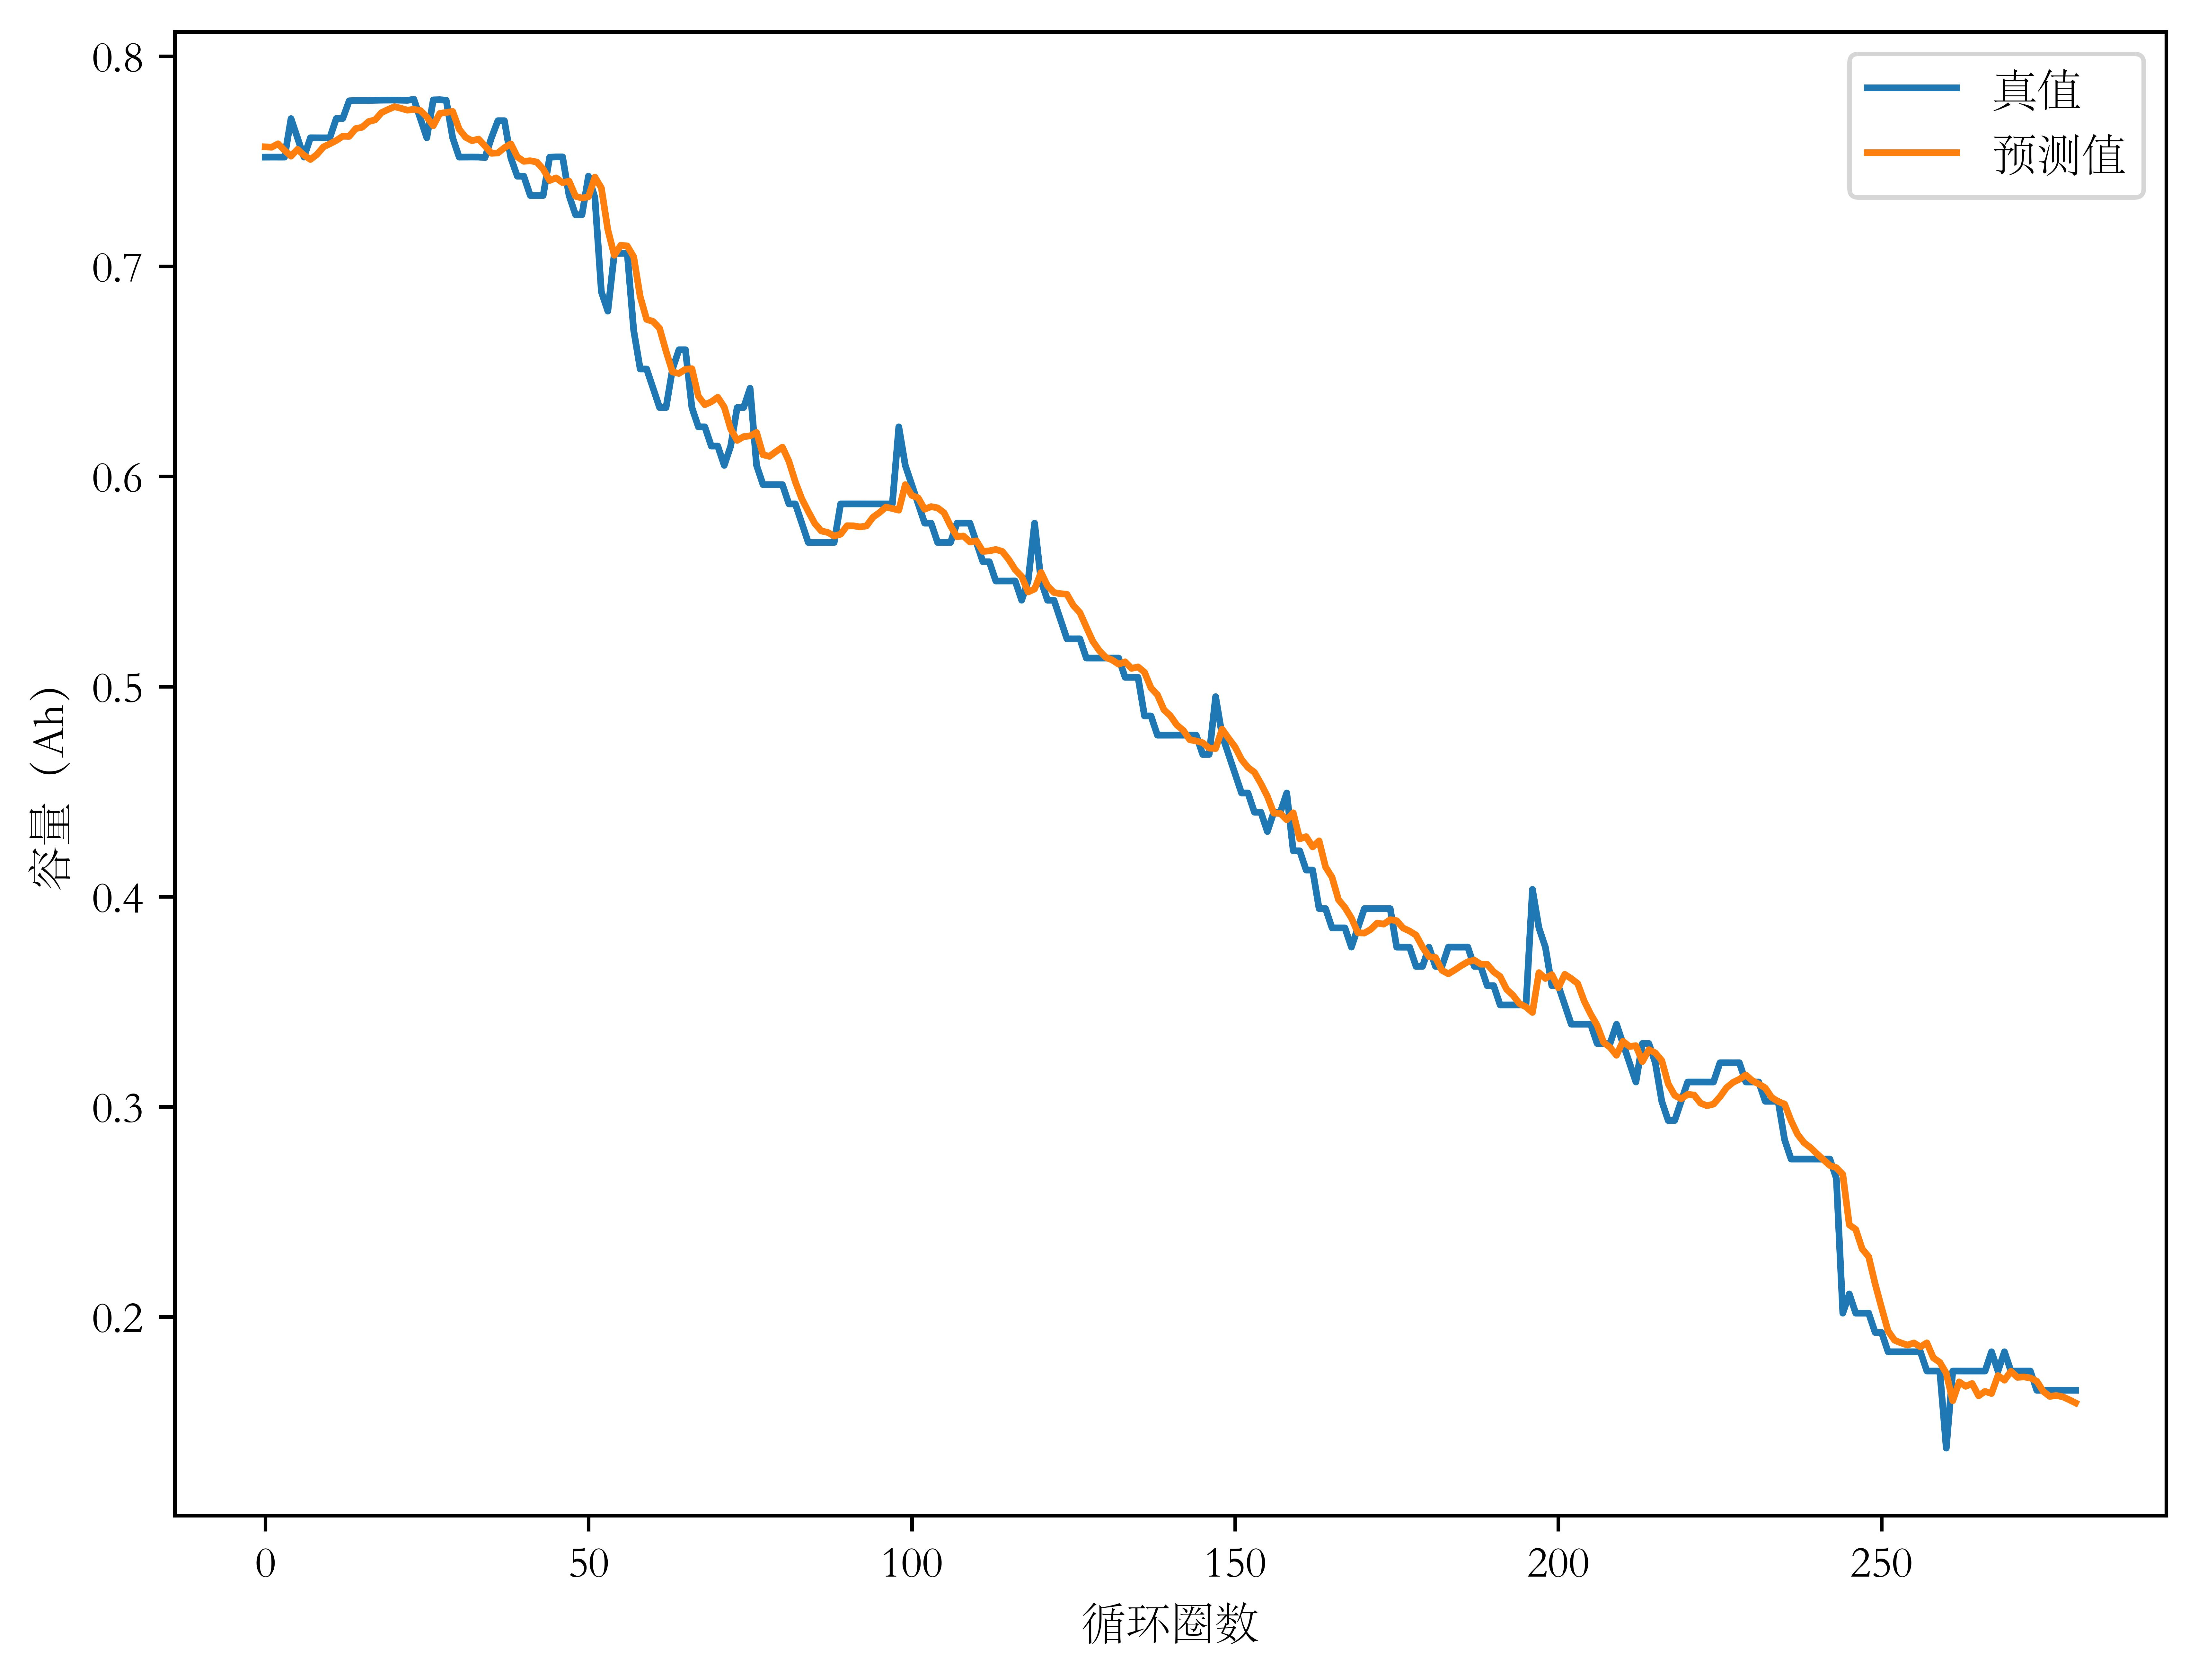
\includegraphics[width=0.15\textwidth]{figures/soh_cap/calce_CS2_36_ar.jpg}}
			{\label{fig:subfig2}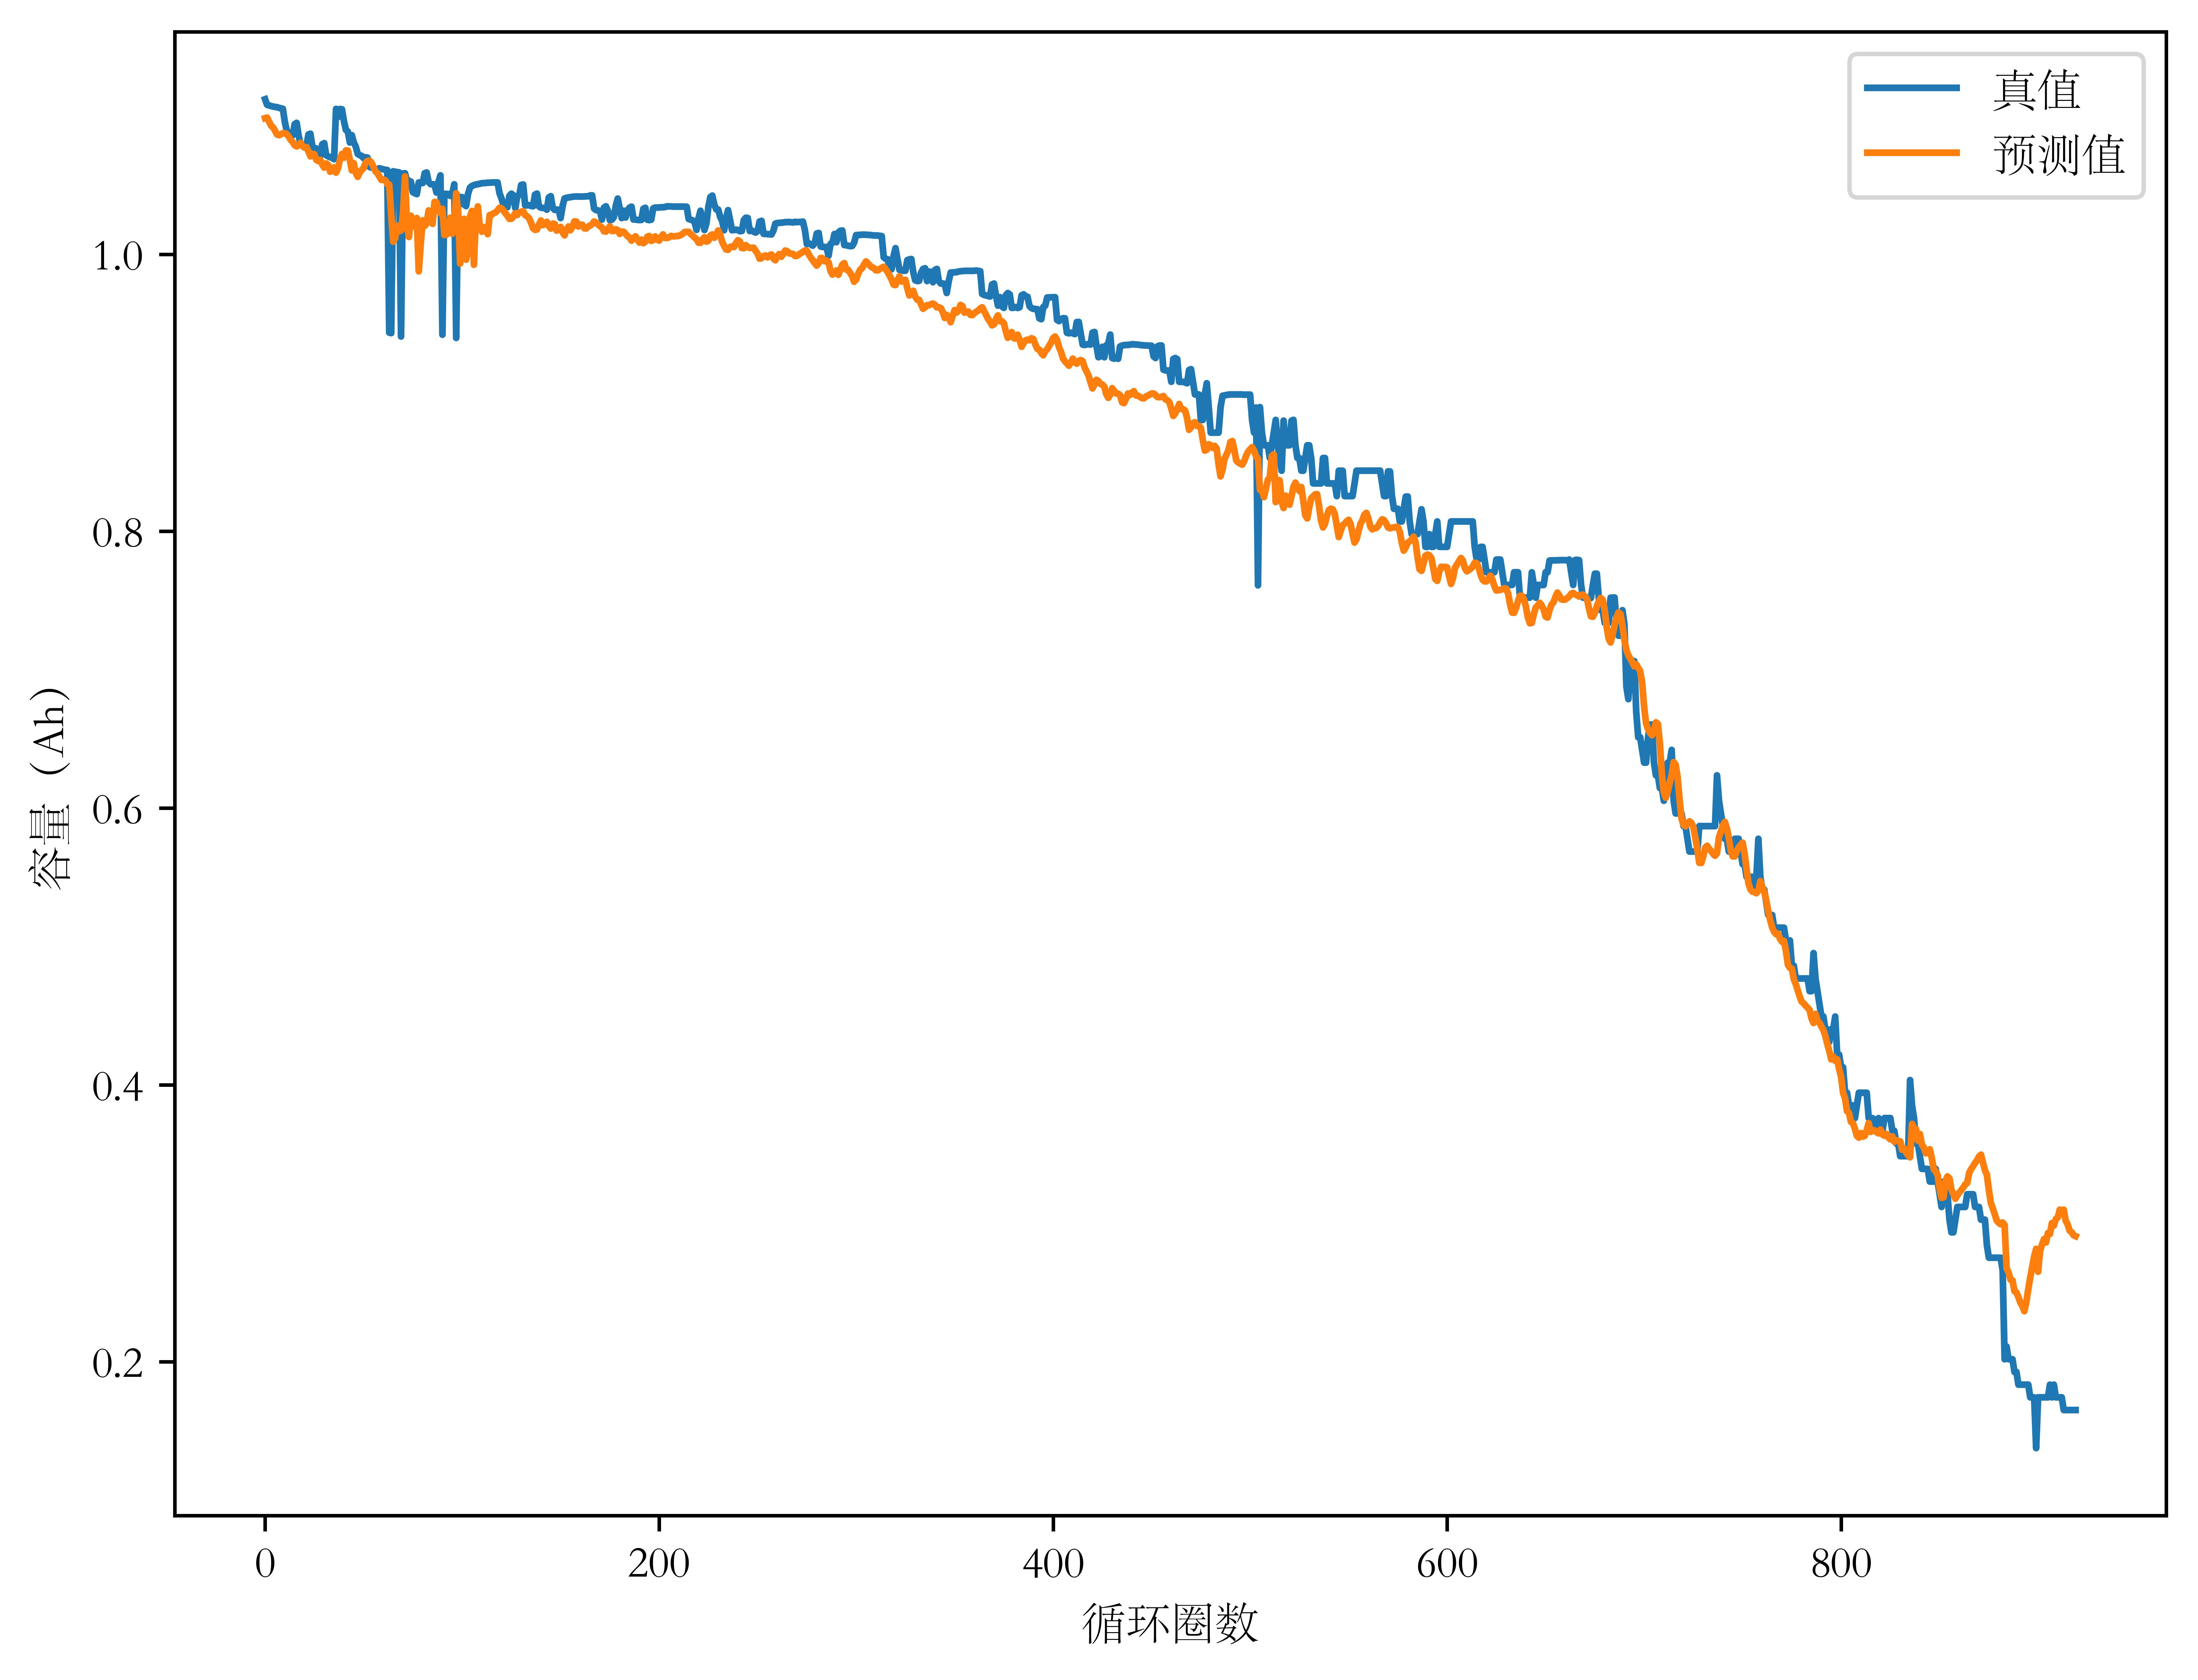
\includegraphics[width=0.15\textwidth]{figures/soh_cap/calce_CS2_36_svr.jpg}}
			{\label{fig:subfig3}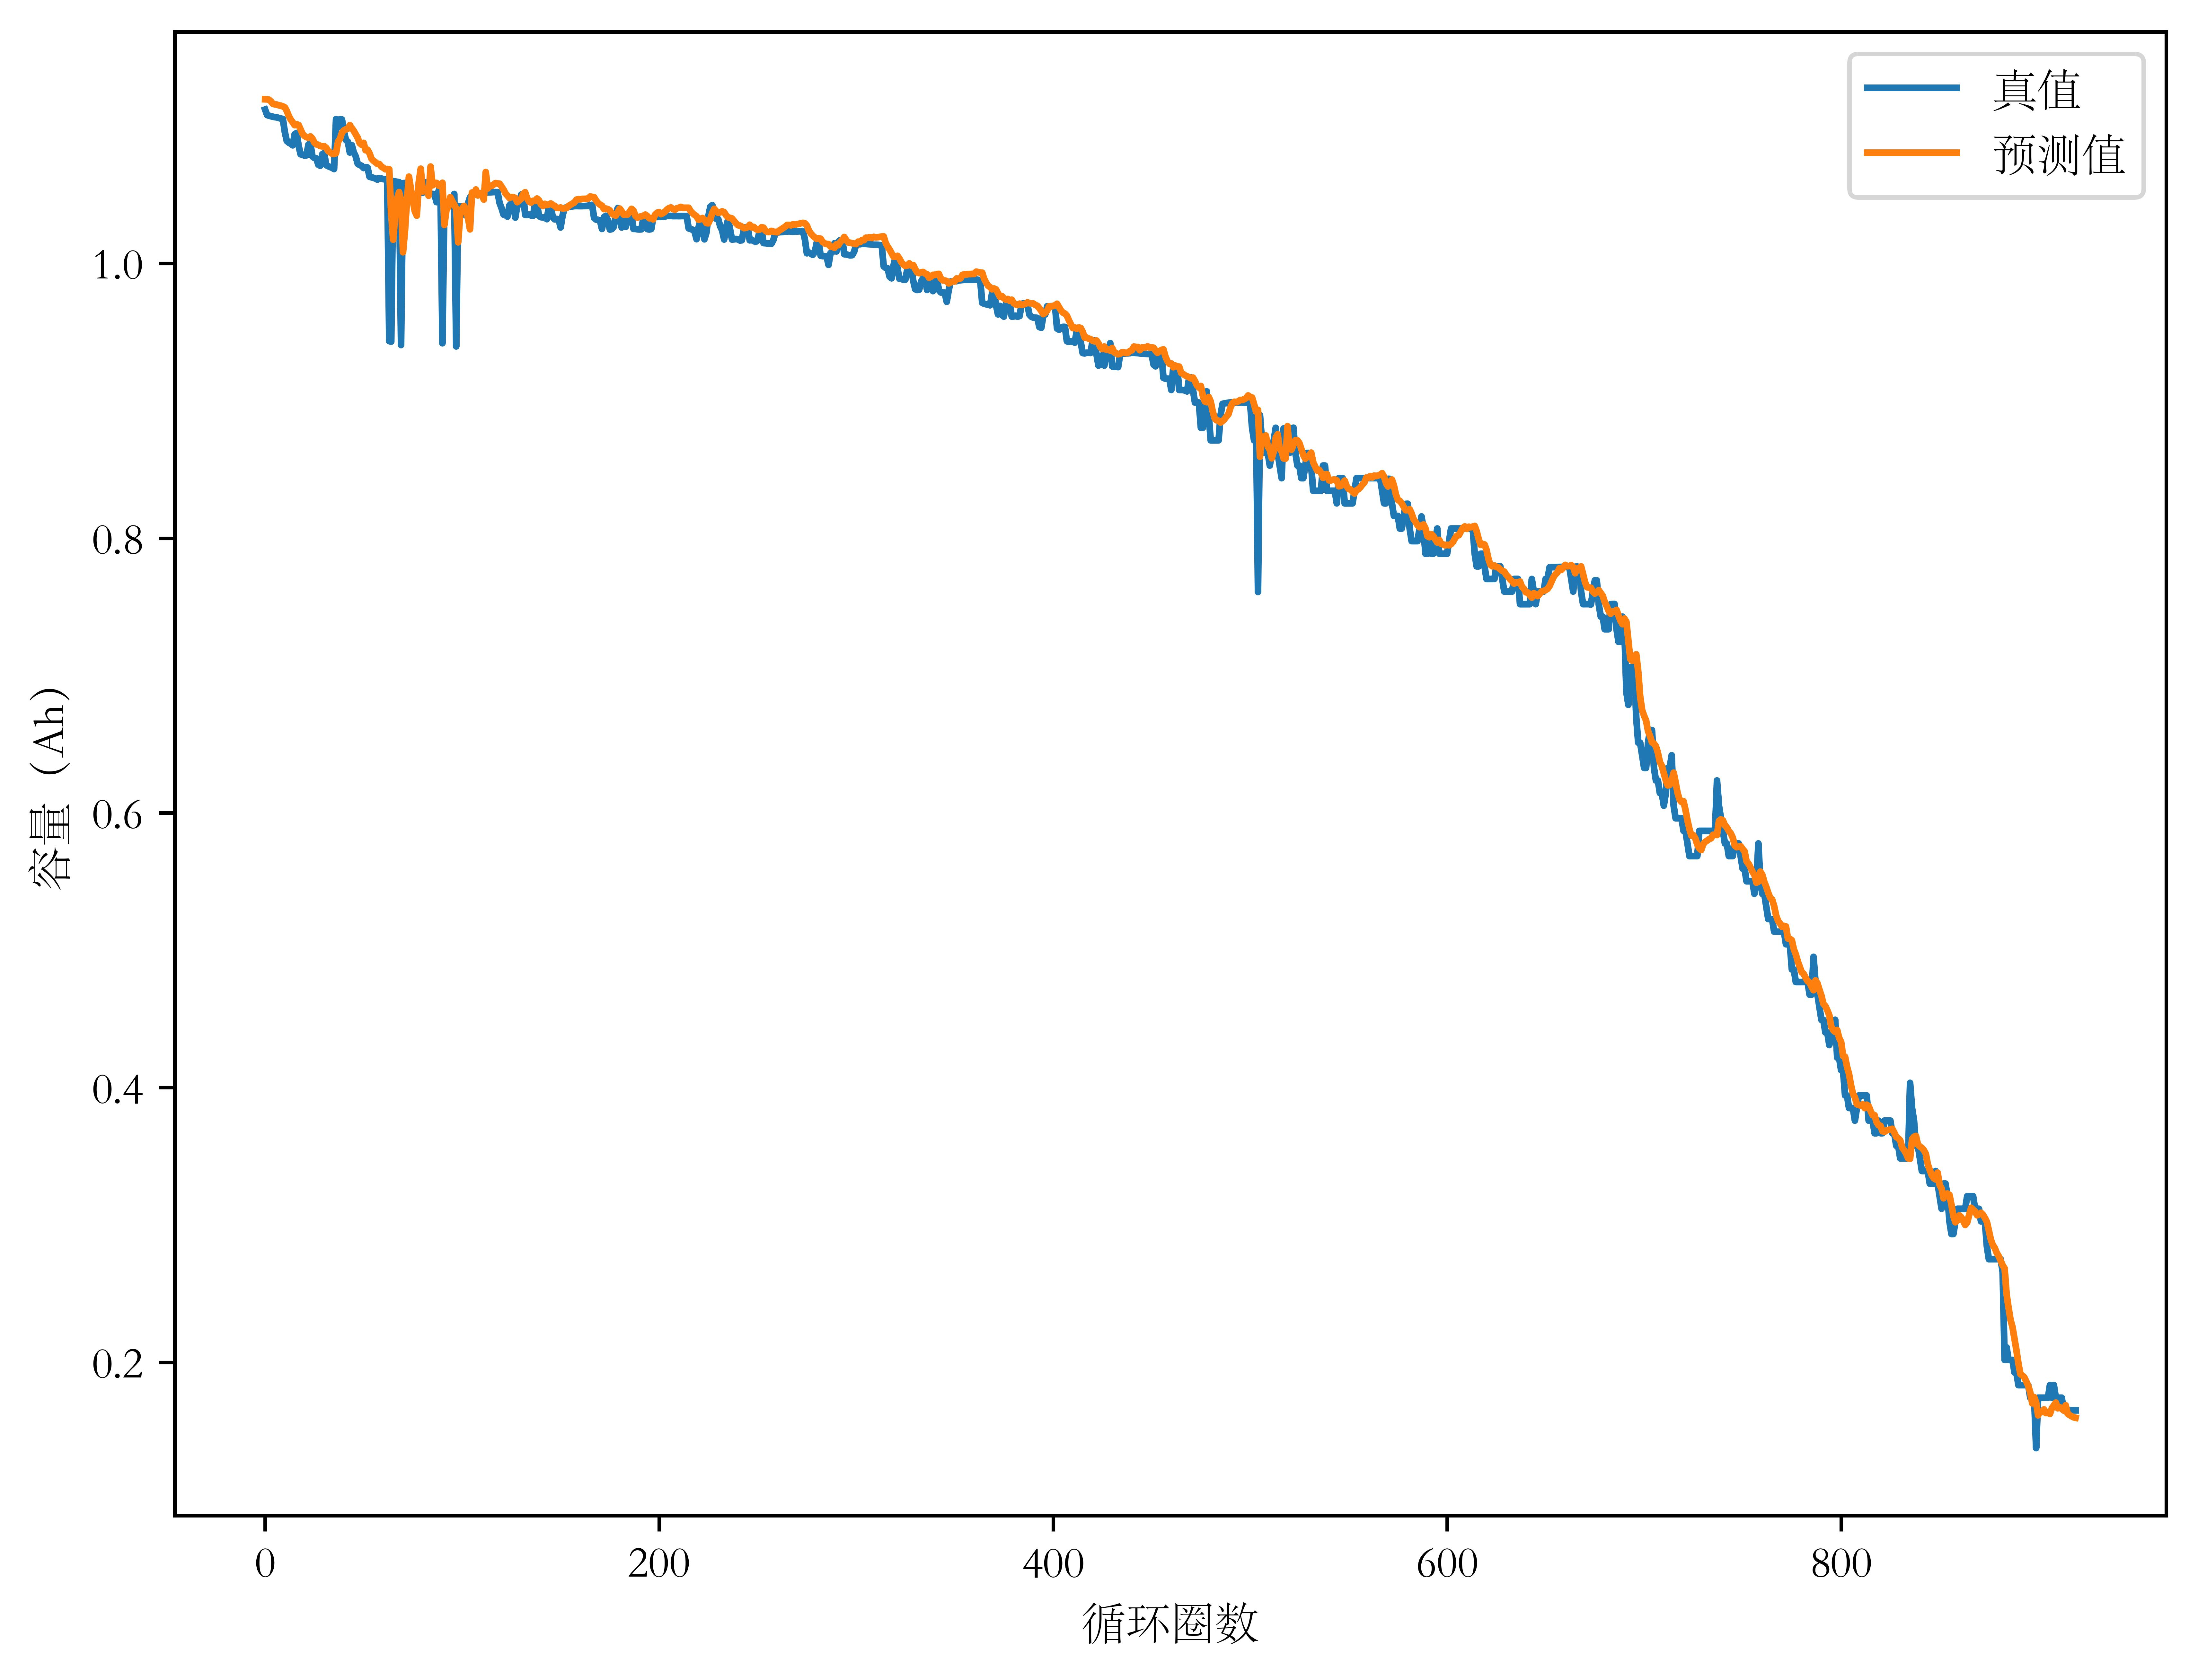
\includegraphics[width=0.15\textwidth]{figures/soh_cap/calce_CS2_36_mlp.jpg}}
			{\label{fig:subfig4}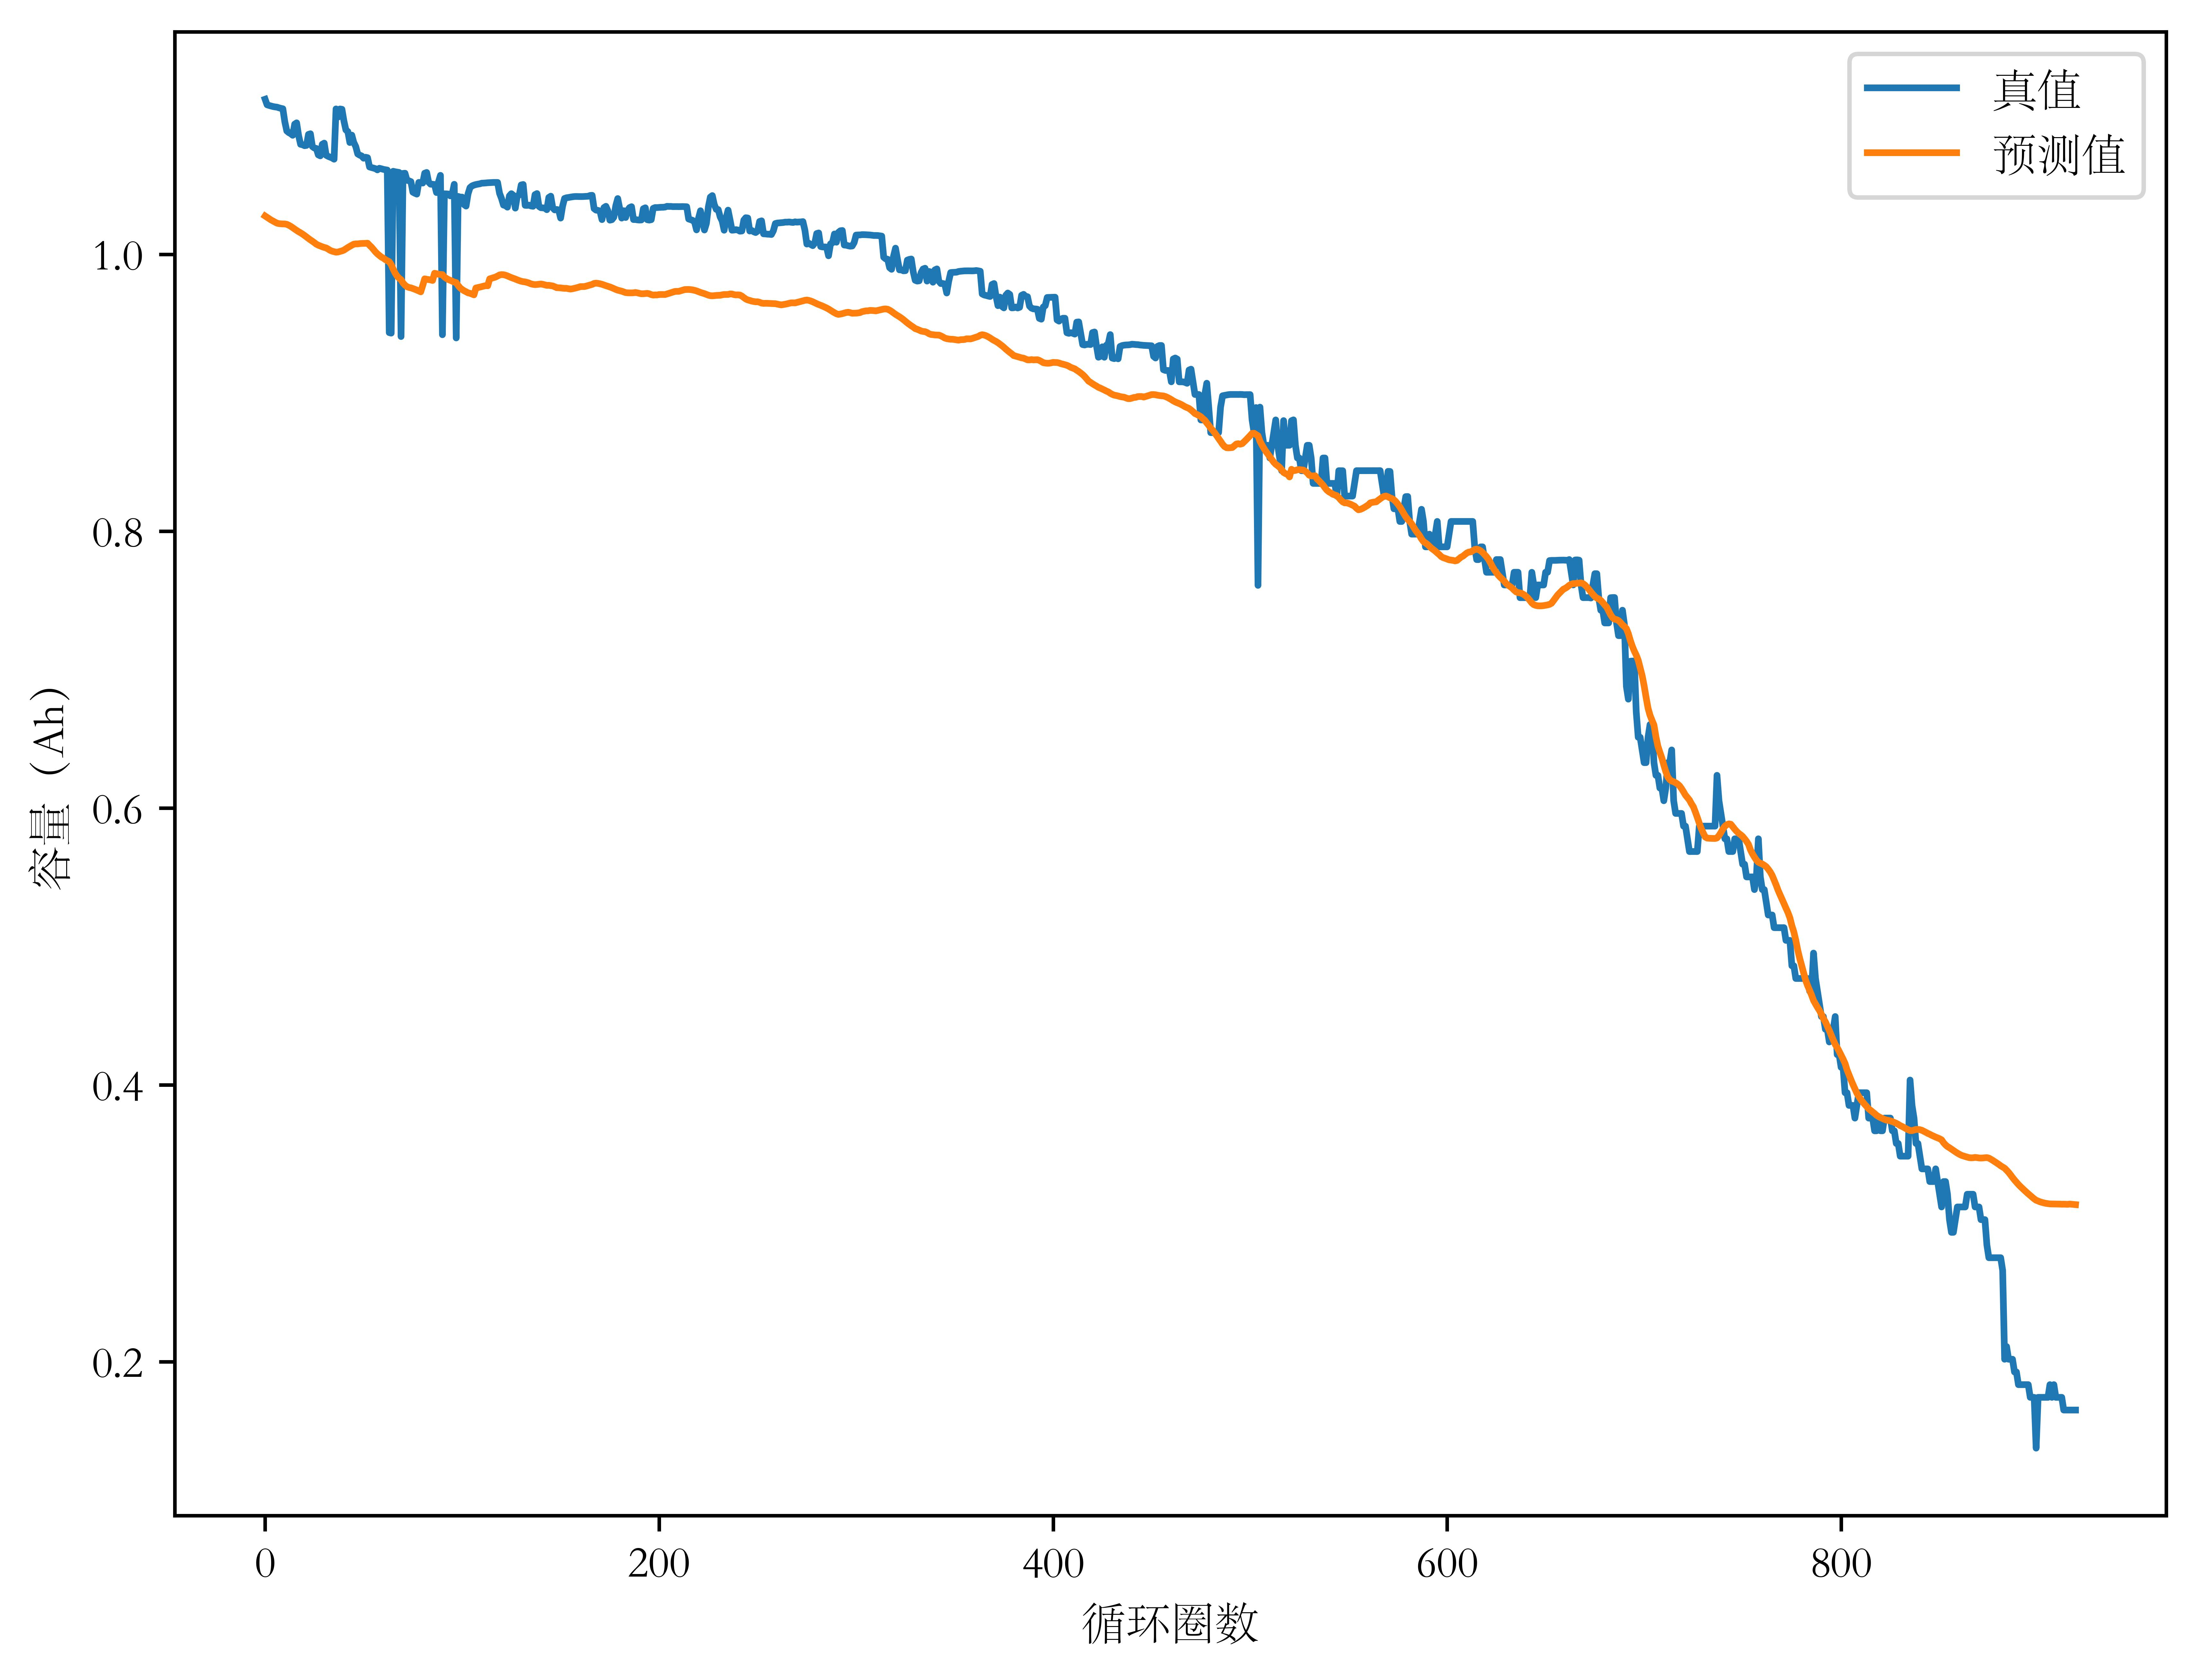
\includegraphics[width=0.15\textwidth]{figures/soh_cap/calce_CS2_36_lstm.jpg}}
			{\label{fig:subfig5}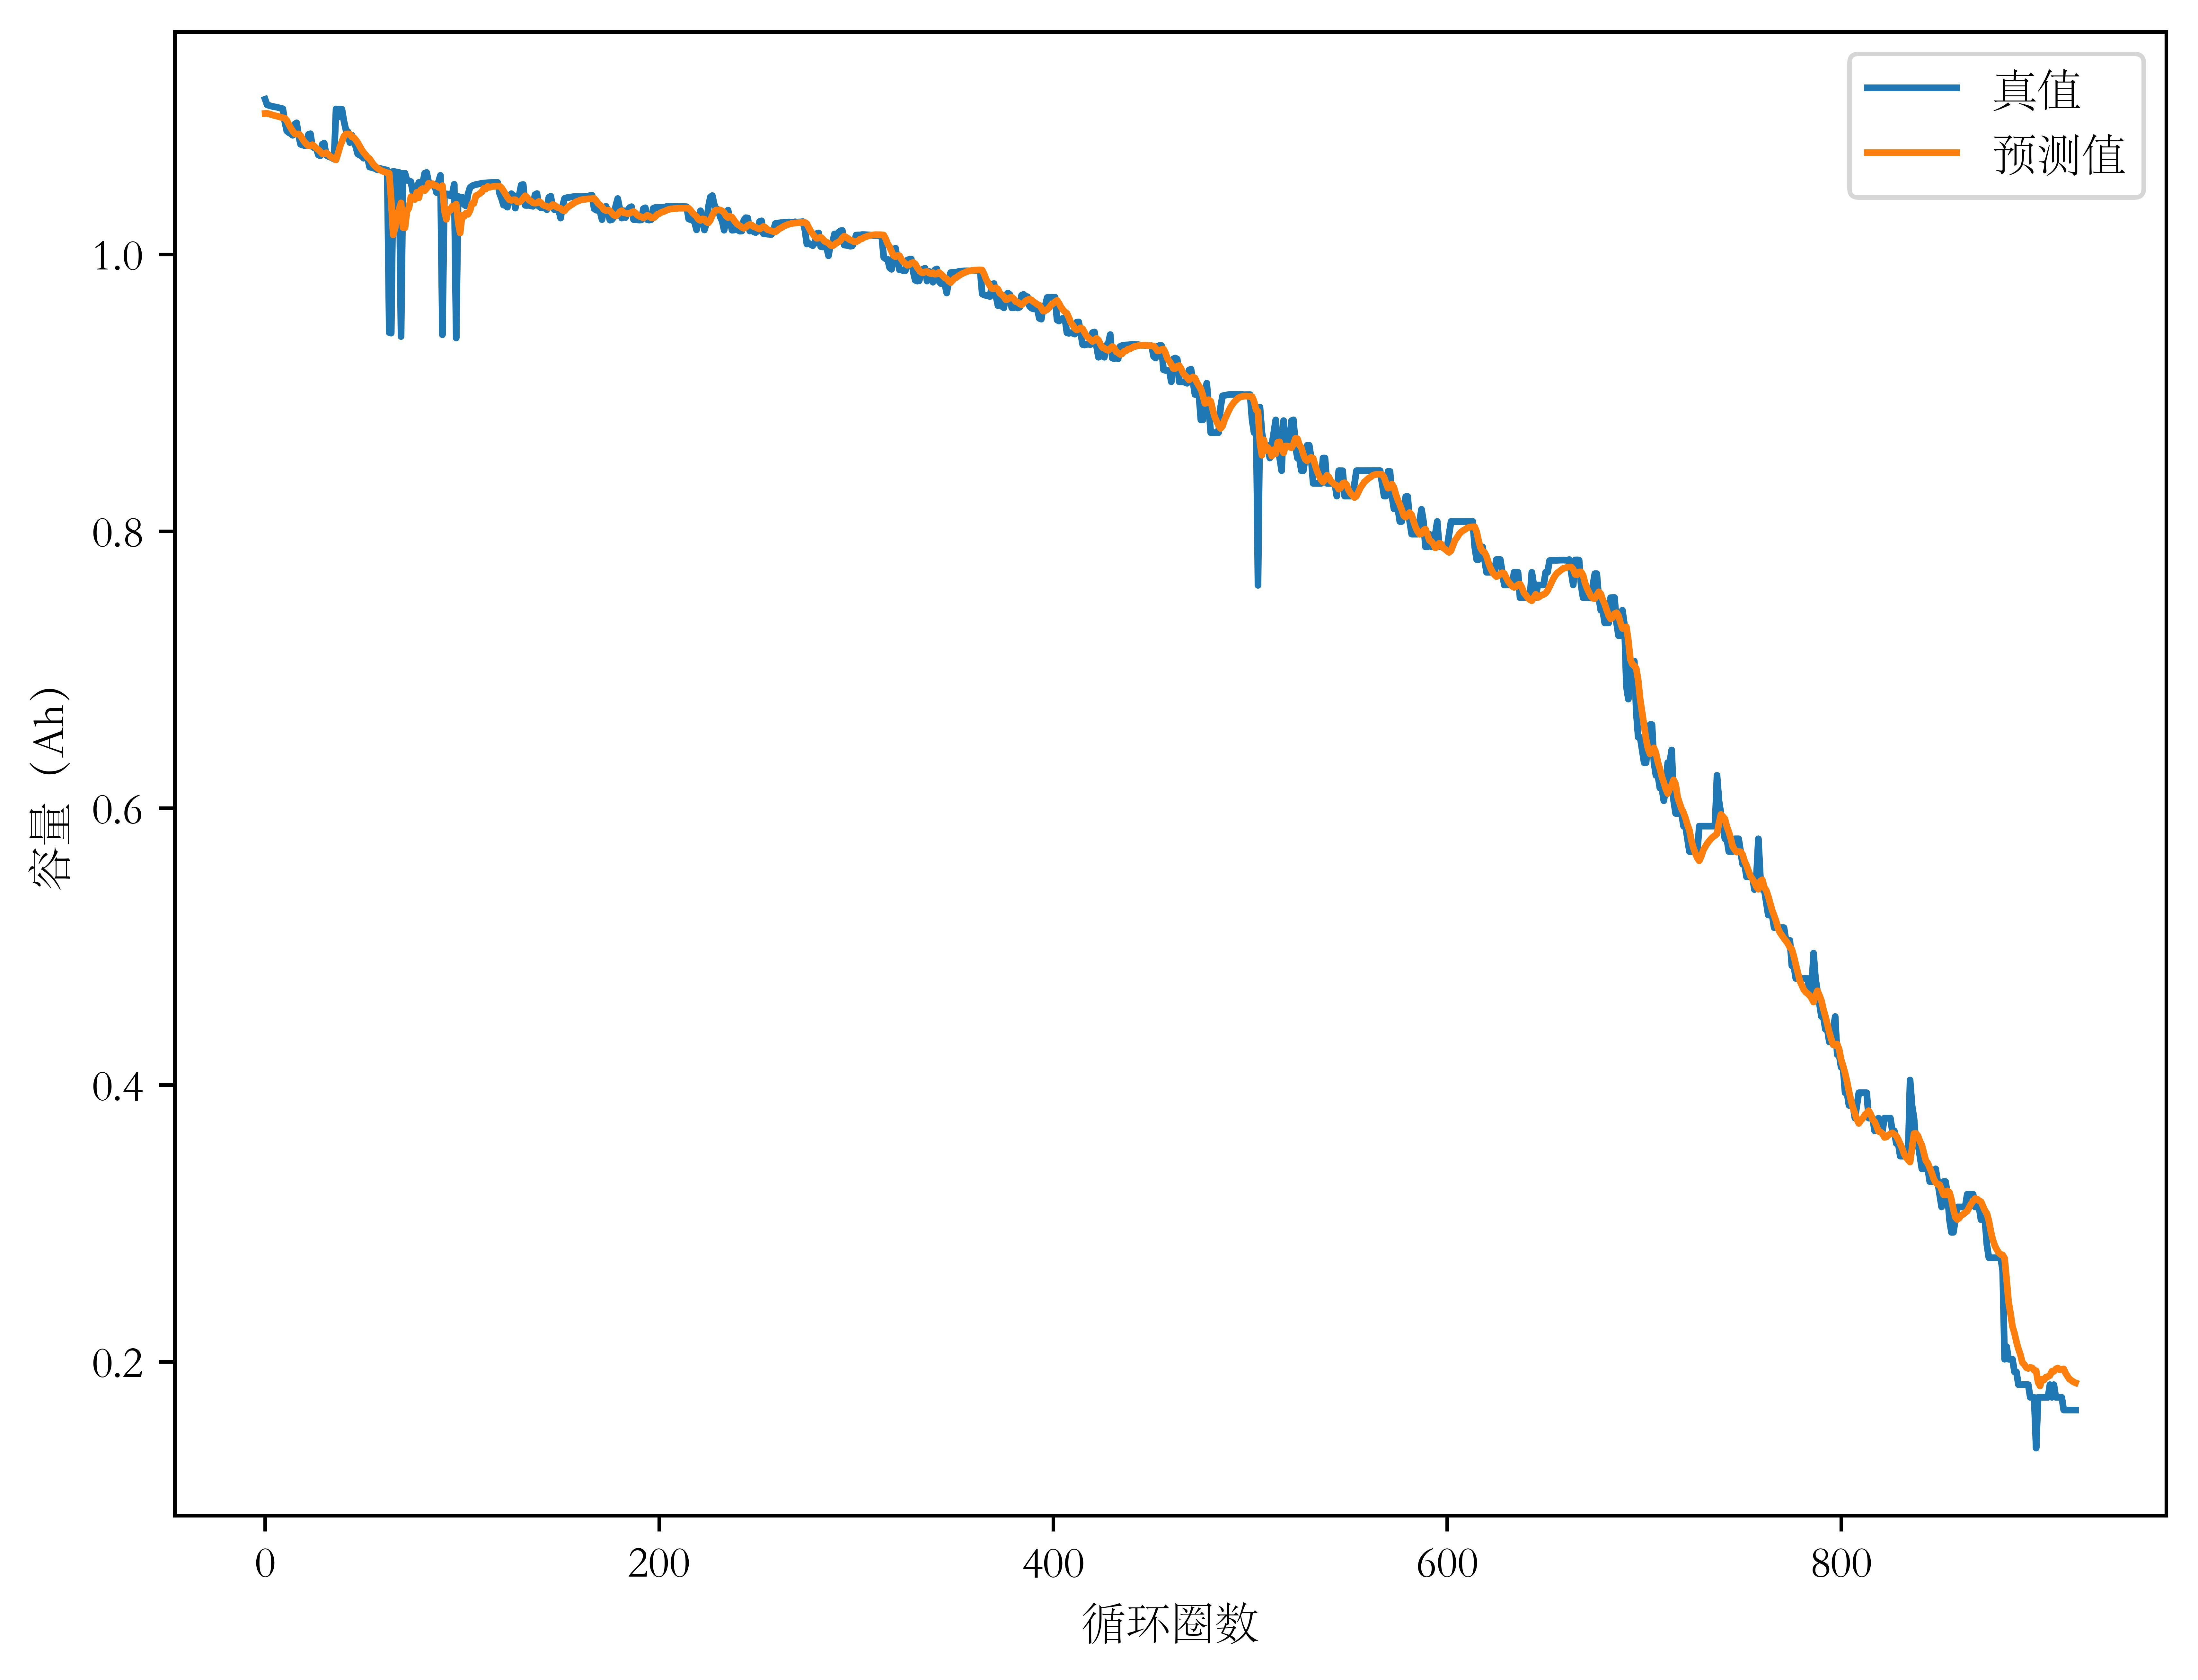
\includegraphics[width=0.15\textwidth]{figures/soh_cap/calce_CS2_36_cnn.jpg}}
	\end{figure}
	\begin{figure}[htbp]
		\centering
			{\label{fig:subfig1}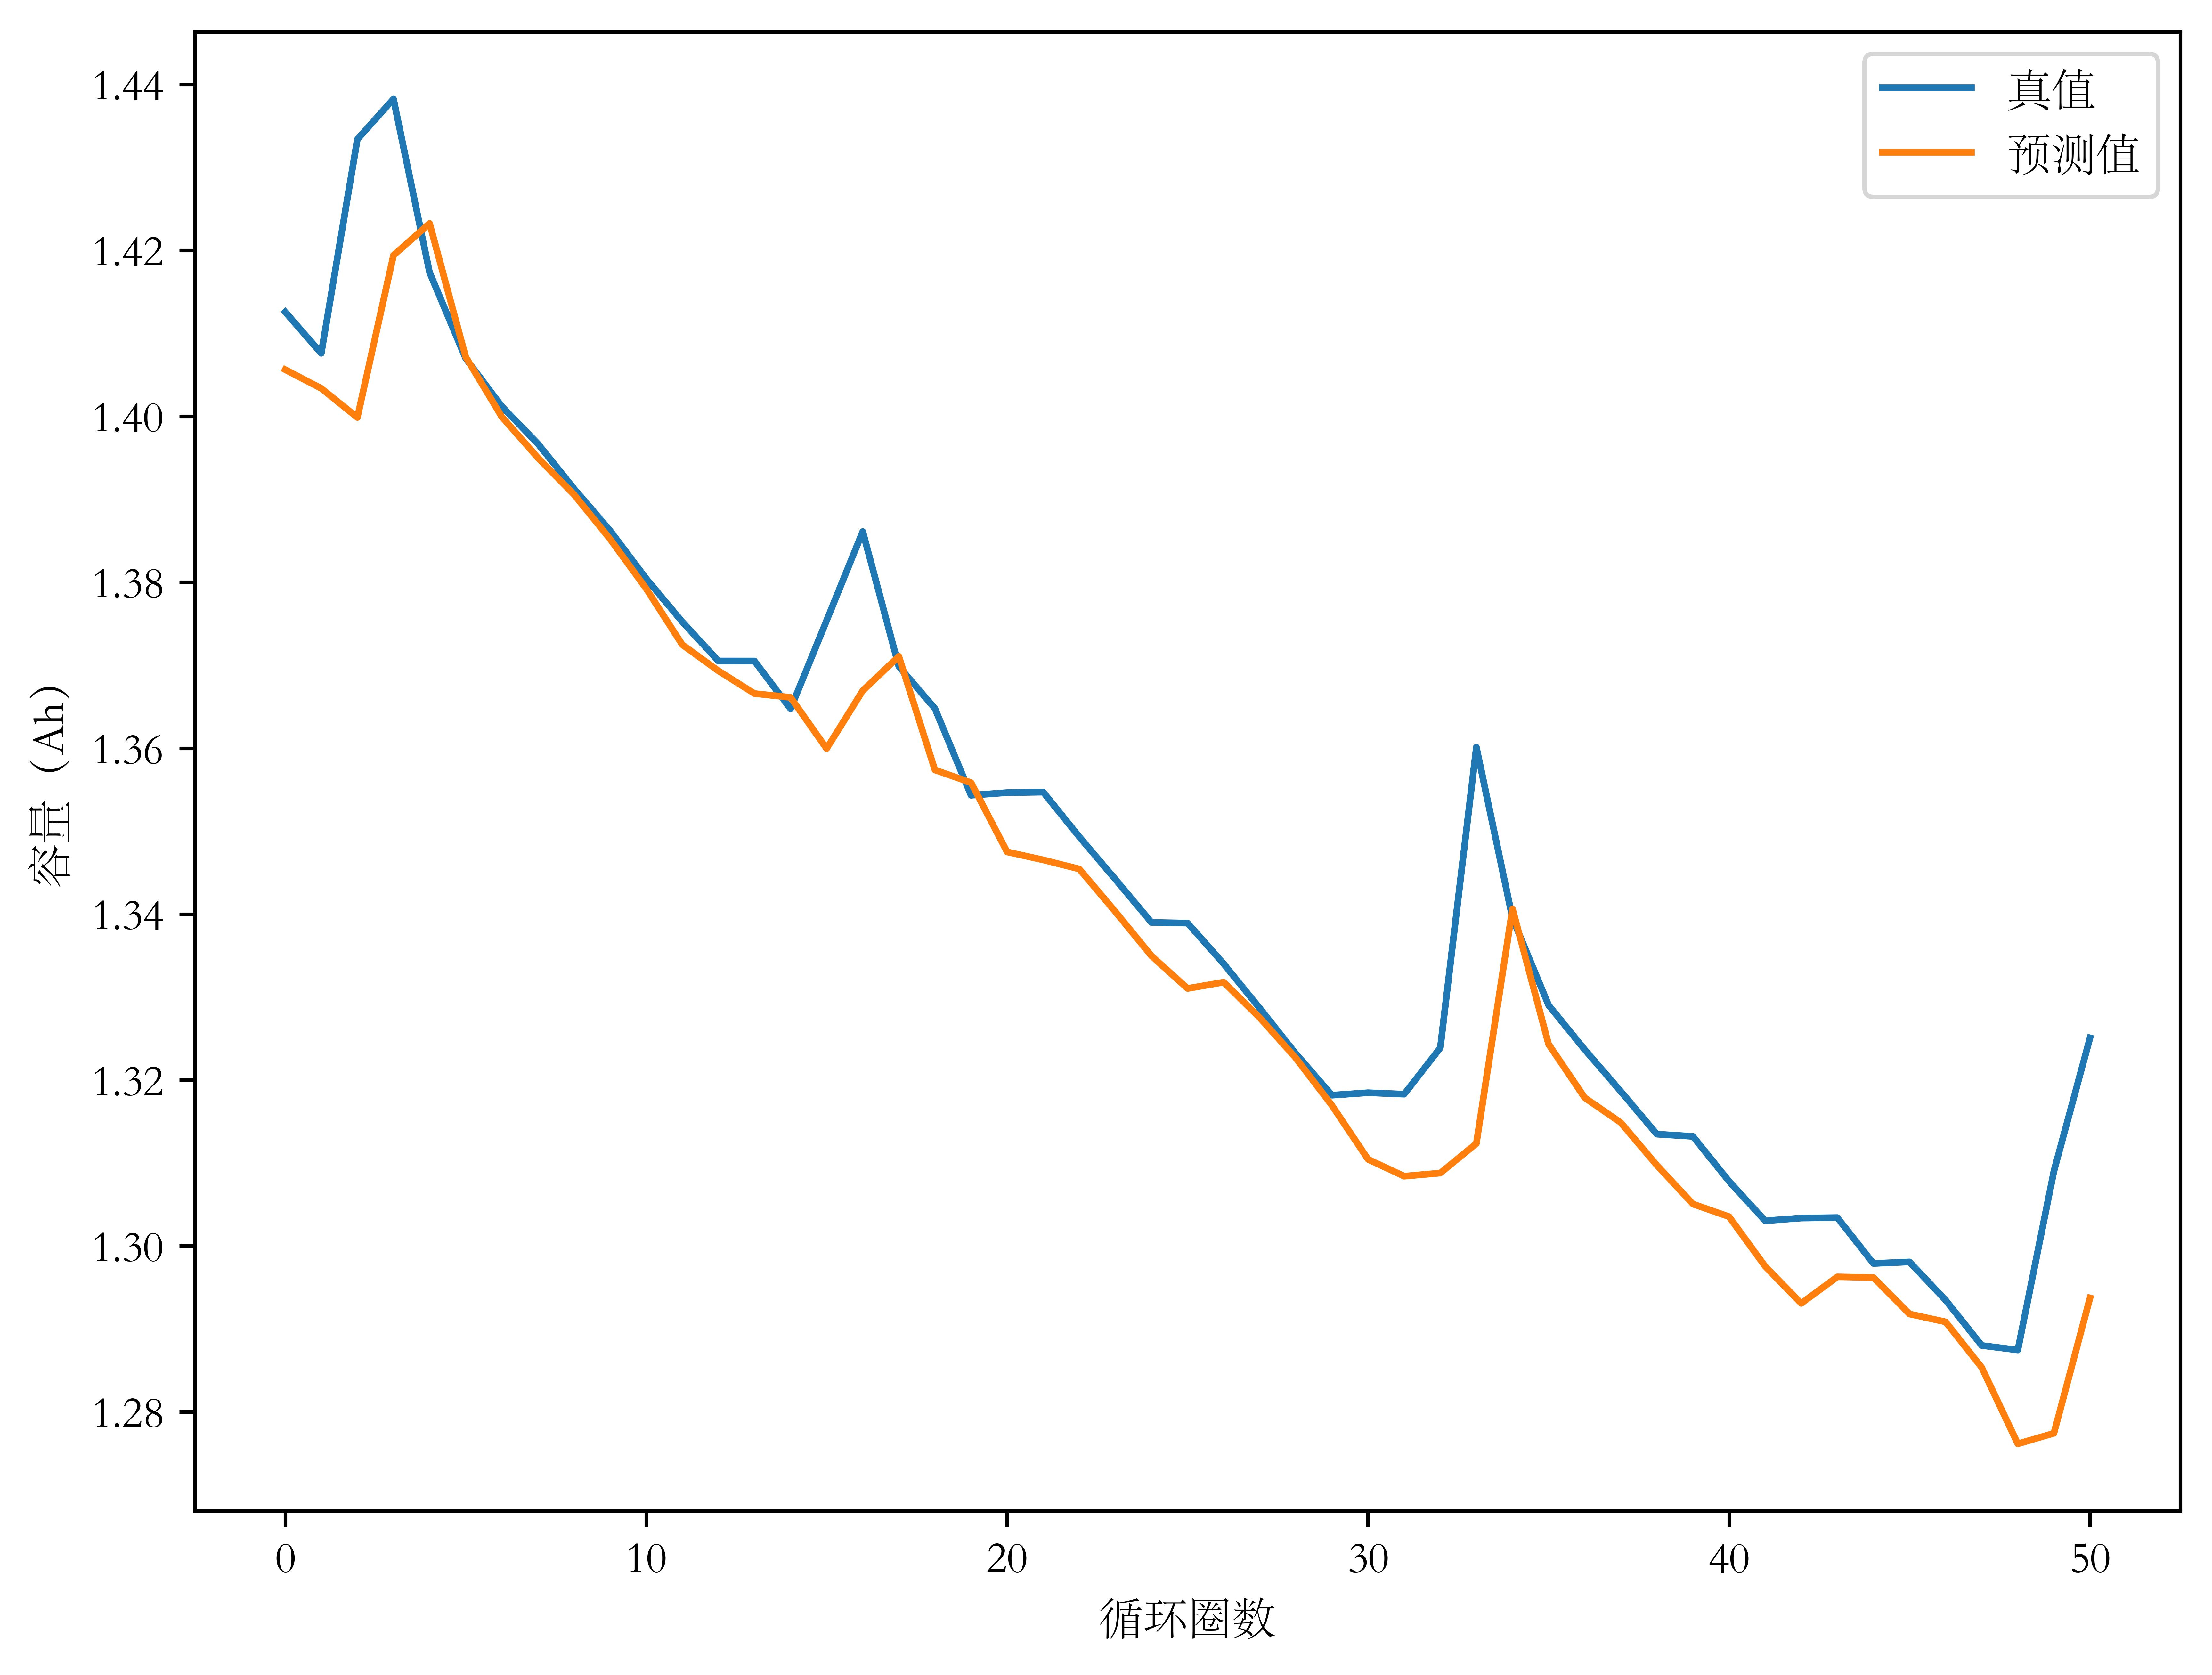
\includegraphics[width=0.15\textwidth]{figures/soh_cap/nasa_B0005_ar.jpg}}
			{\label{fig:subfig2}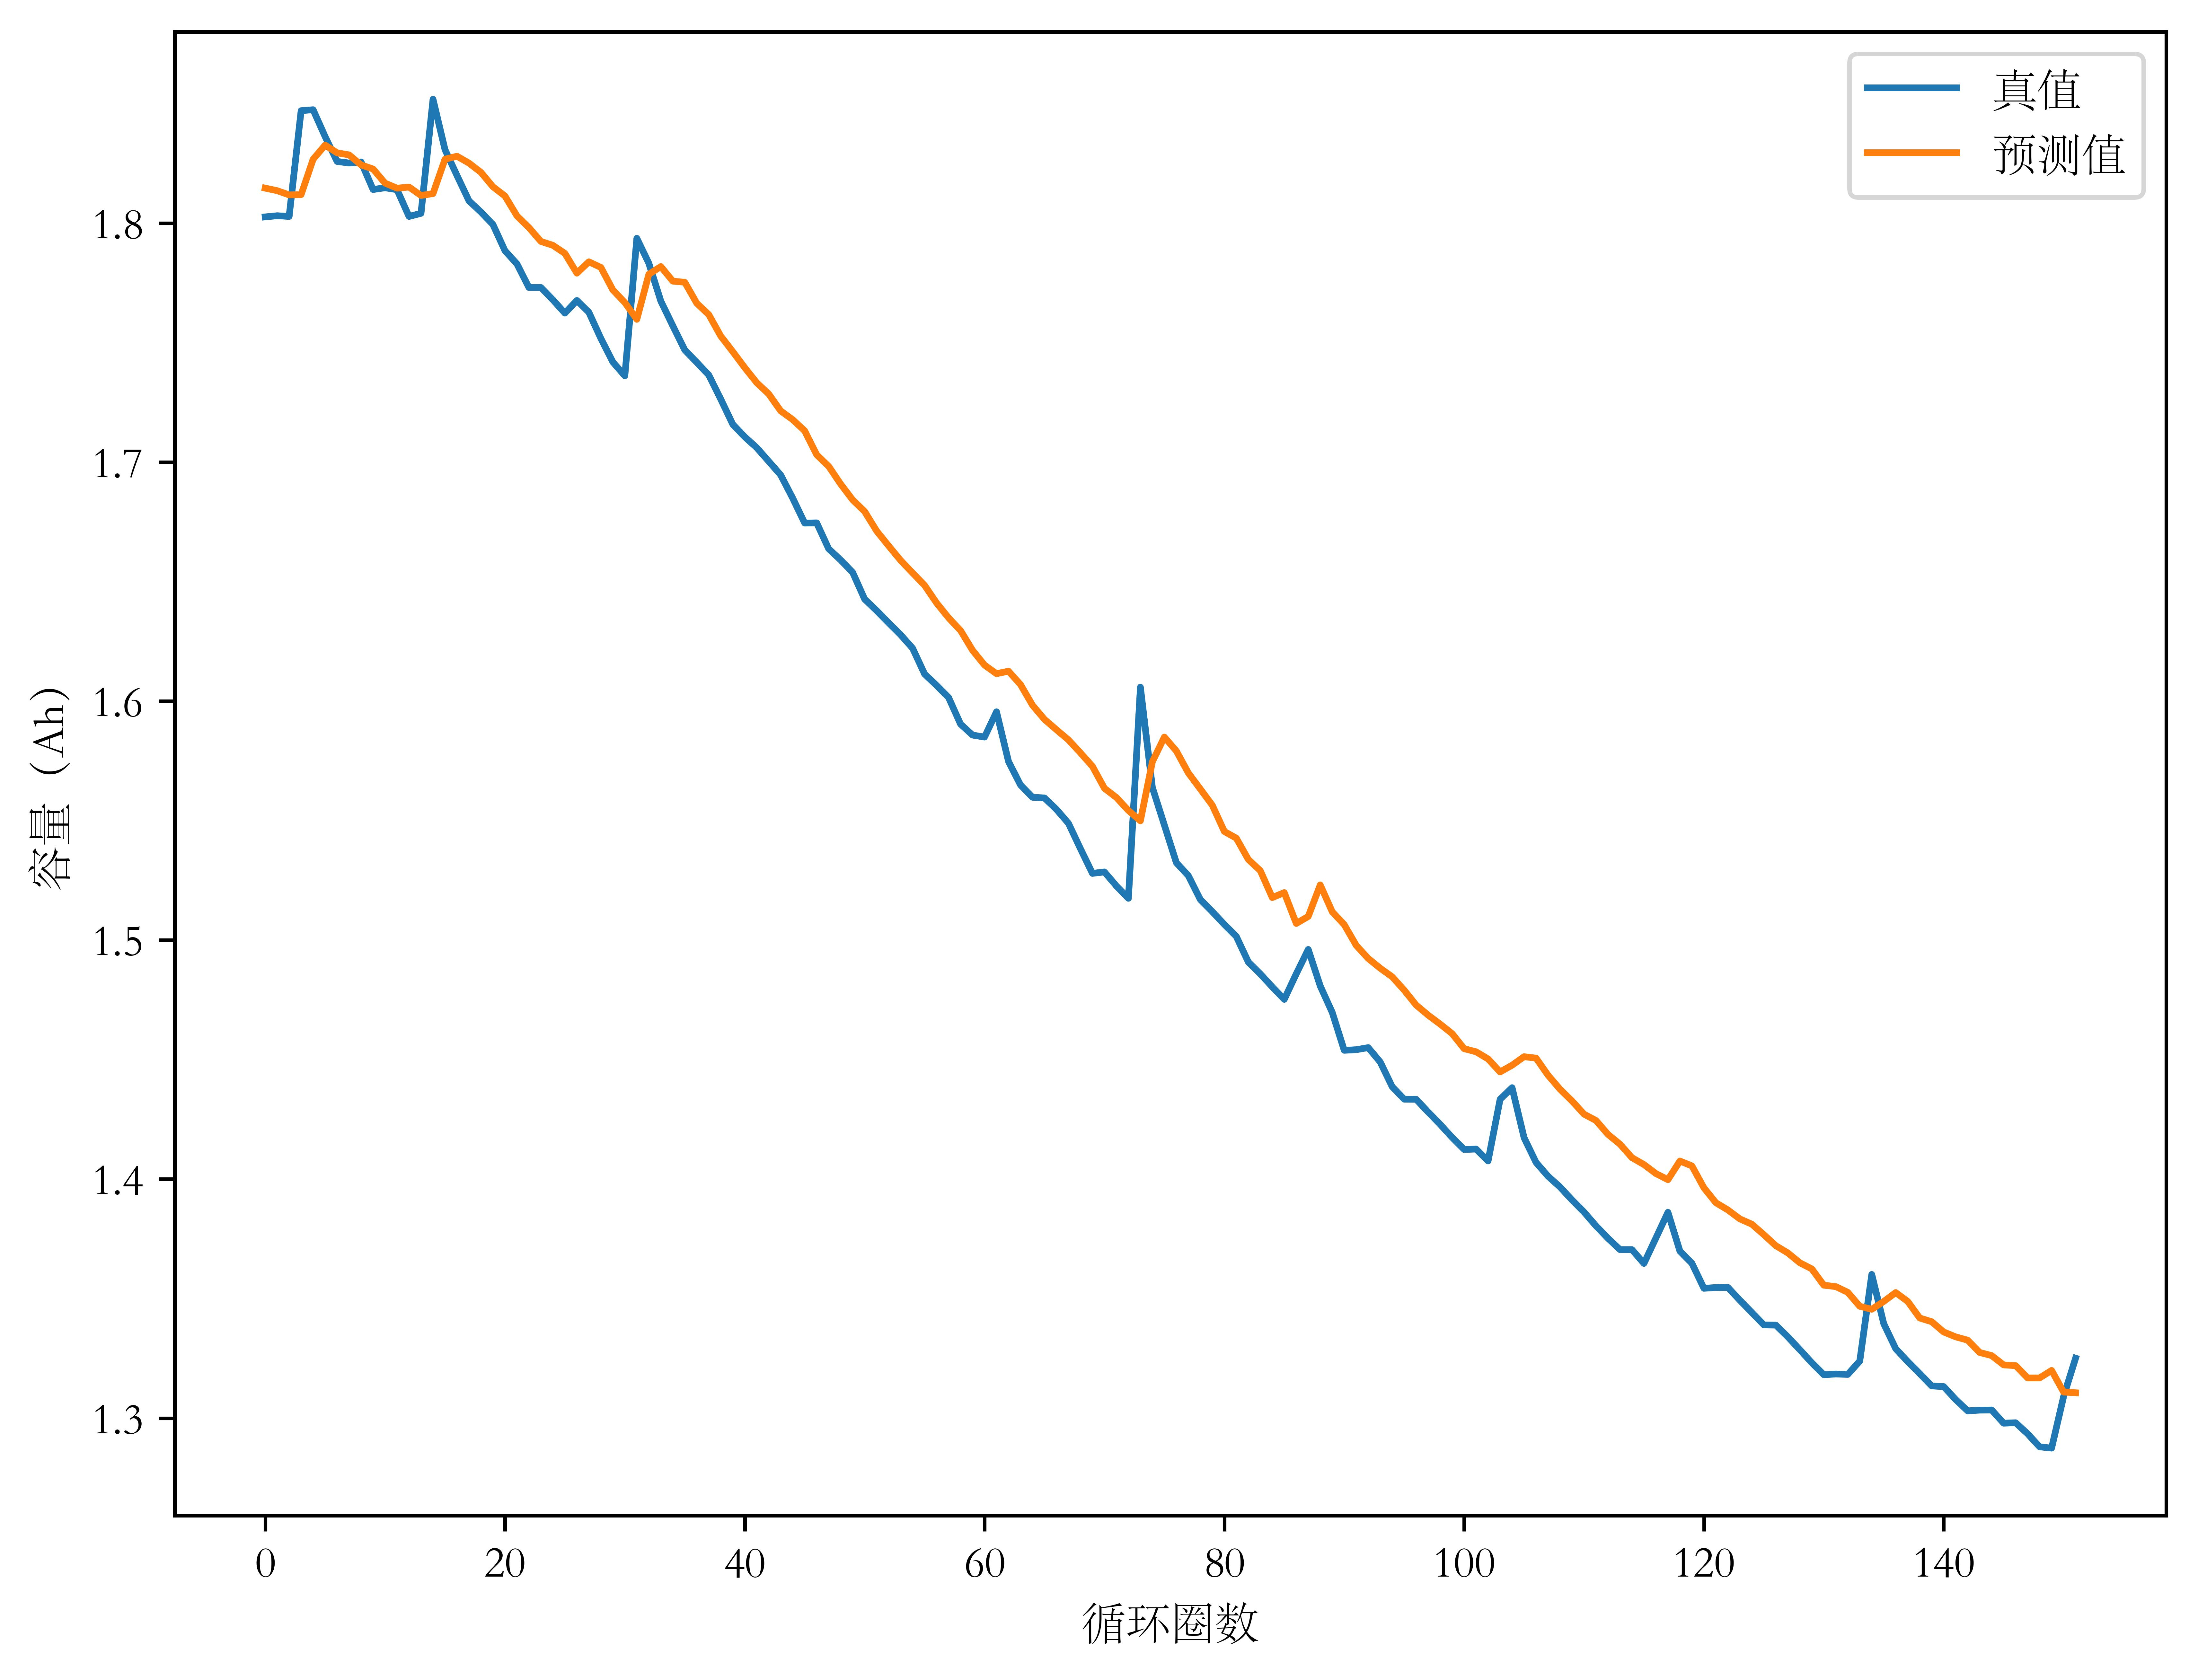
\includegraphics[width=0.15\textwidth]{figures/soh_cap/nasa_B0005_svr.jpg}}
			{\label{fig:subfig3}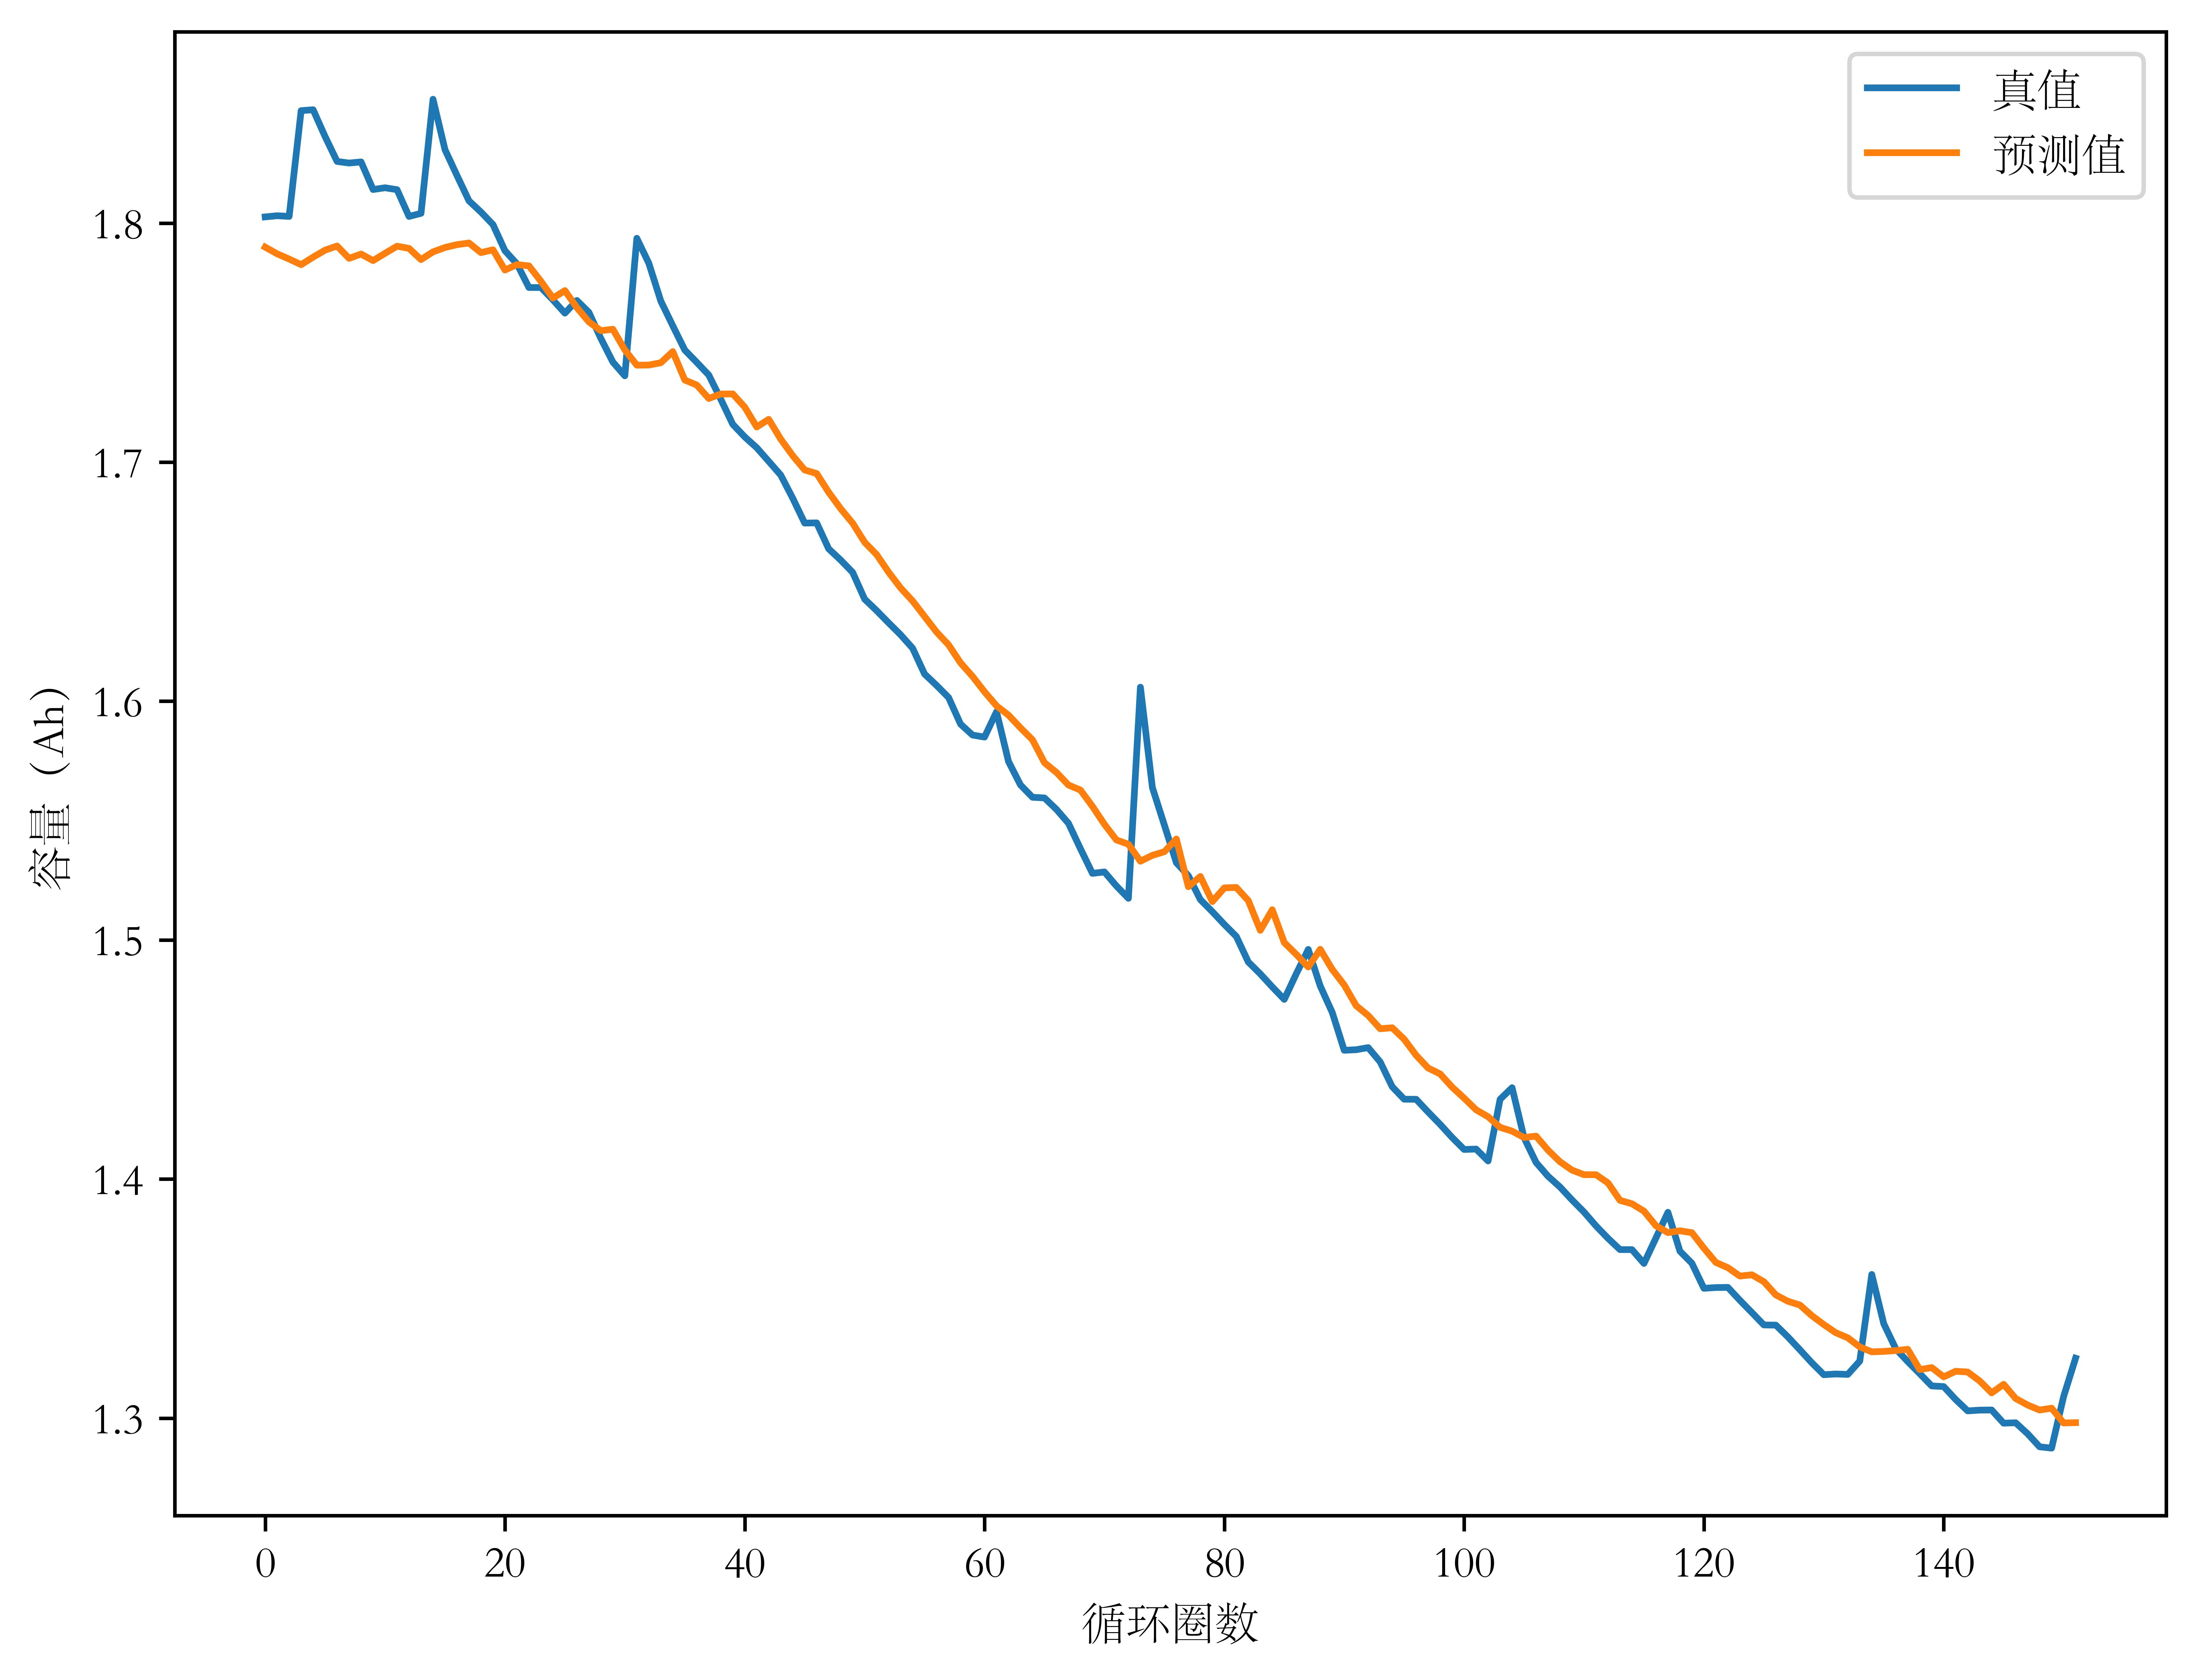
\includegraphics[width=0.15\textwidth]{figures/soh_cap/nasa_B0005_mlp.jpg}}
			{\label{fig:subfig4}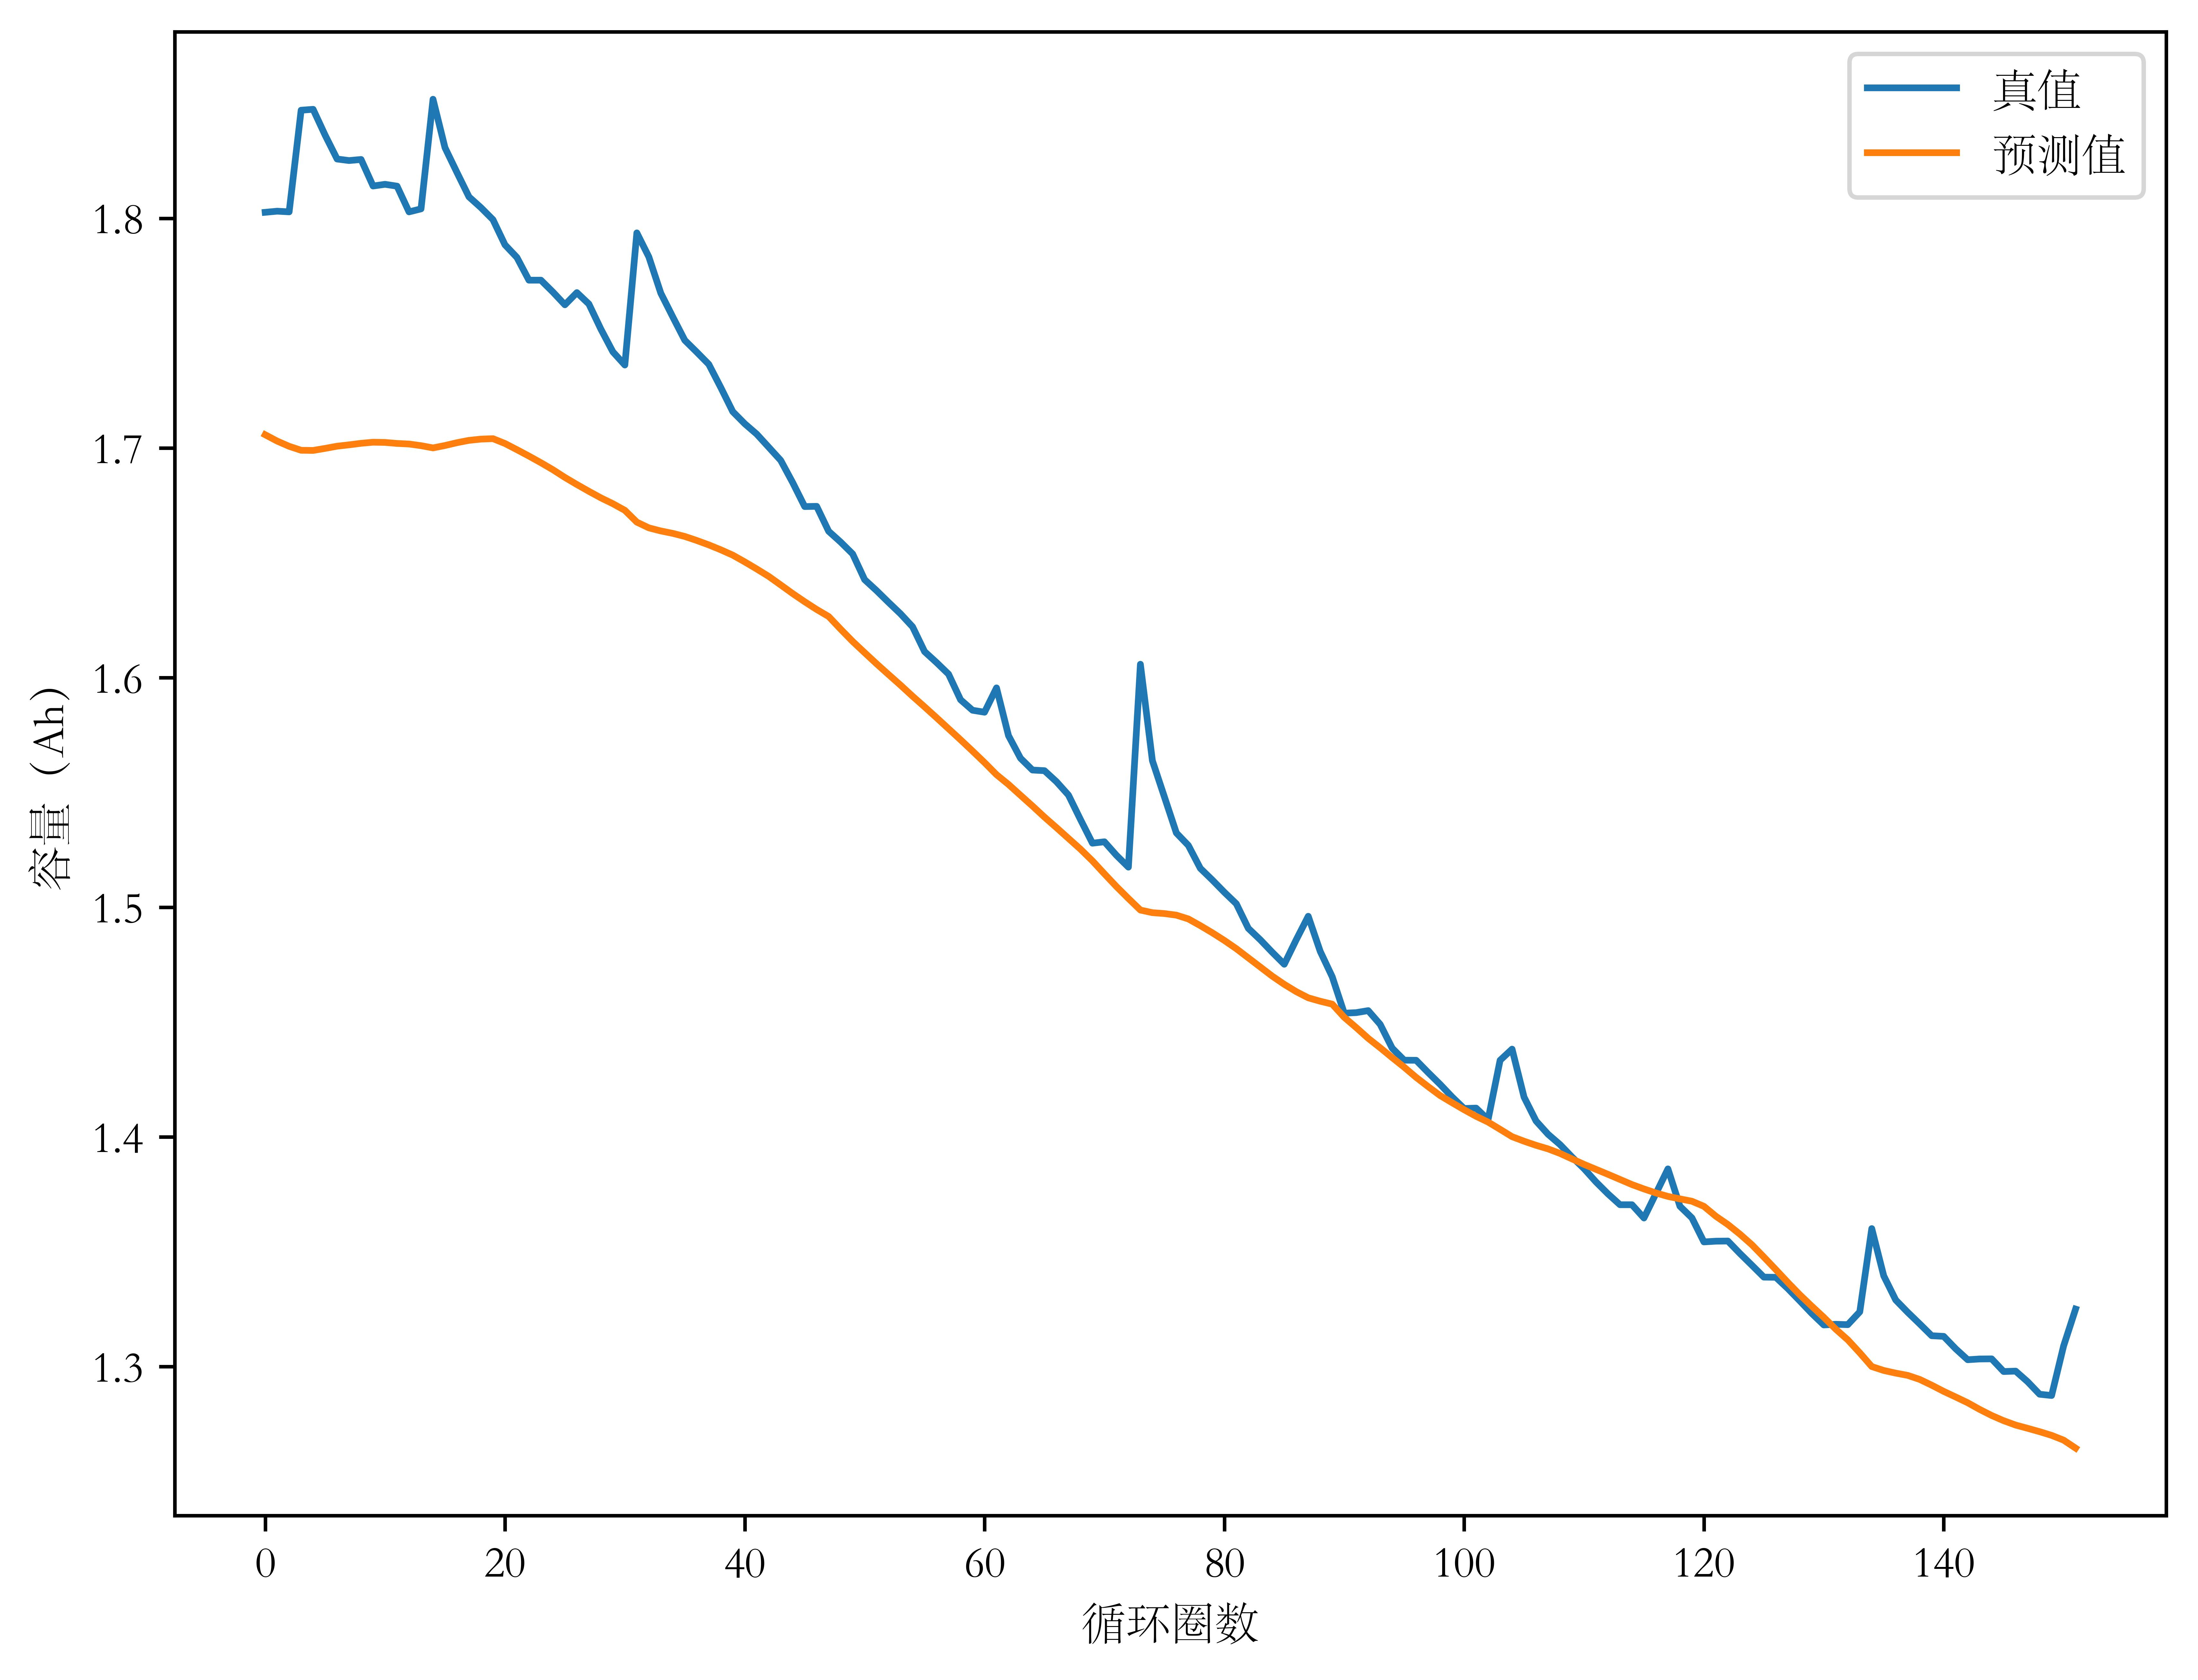
\includegraphics[width=0.15\textwidth]{figures/soh_cap/nasa_B0005_lstm.jpg}}
			{\label{fig:subfig5}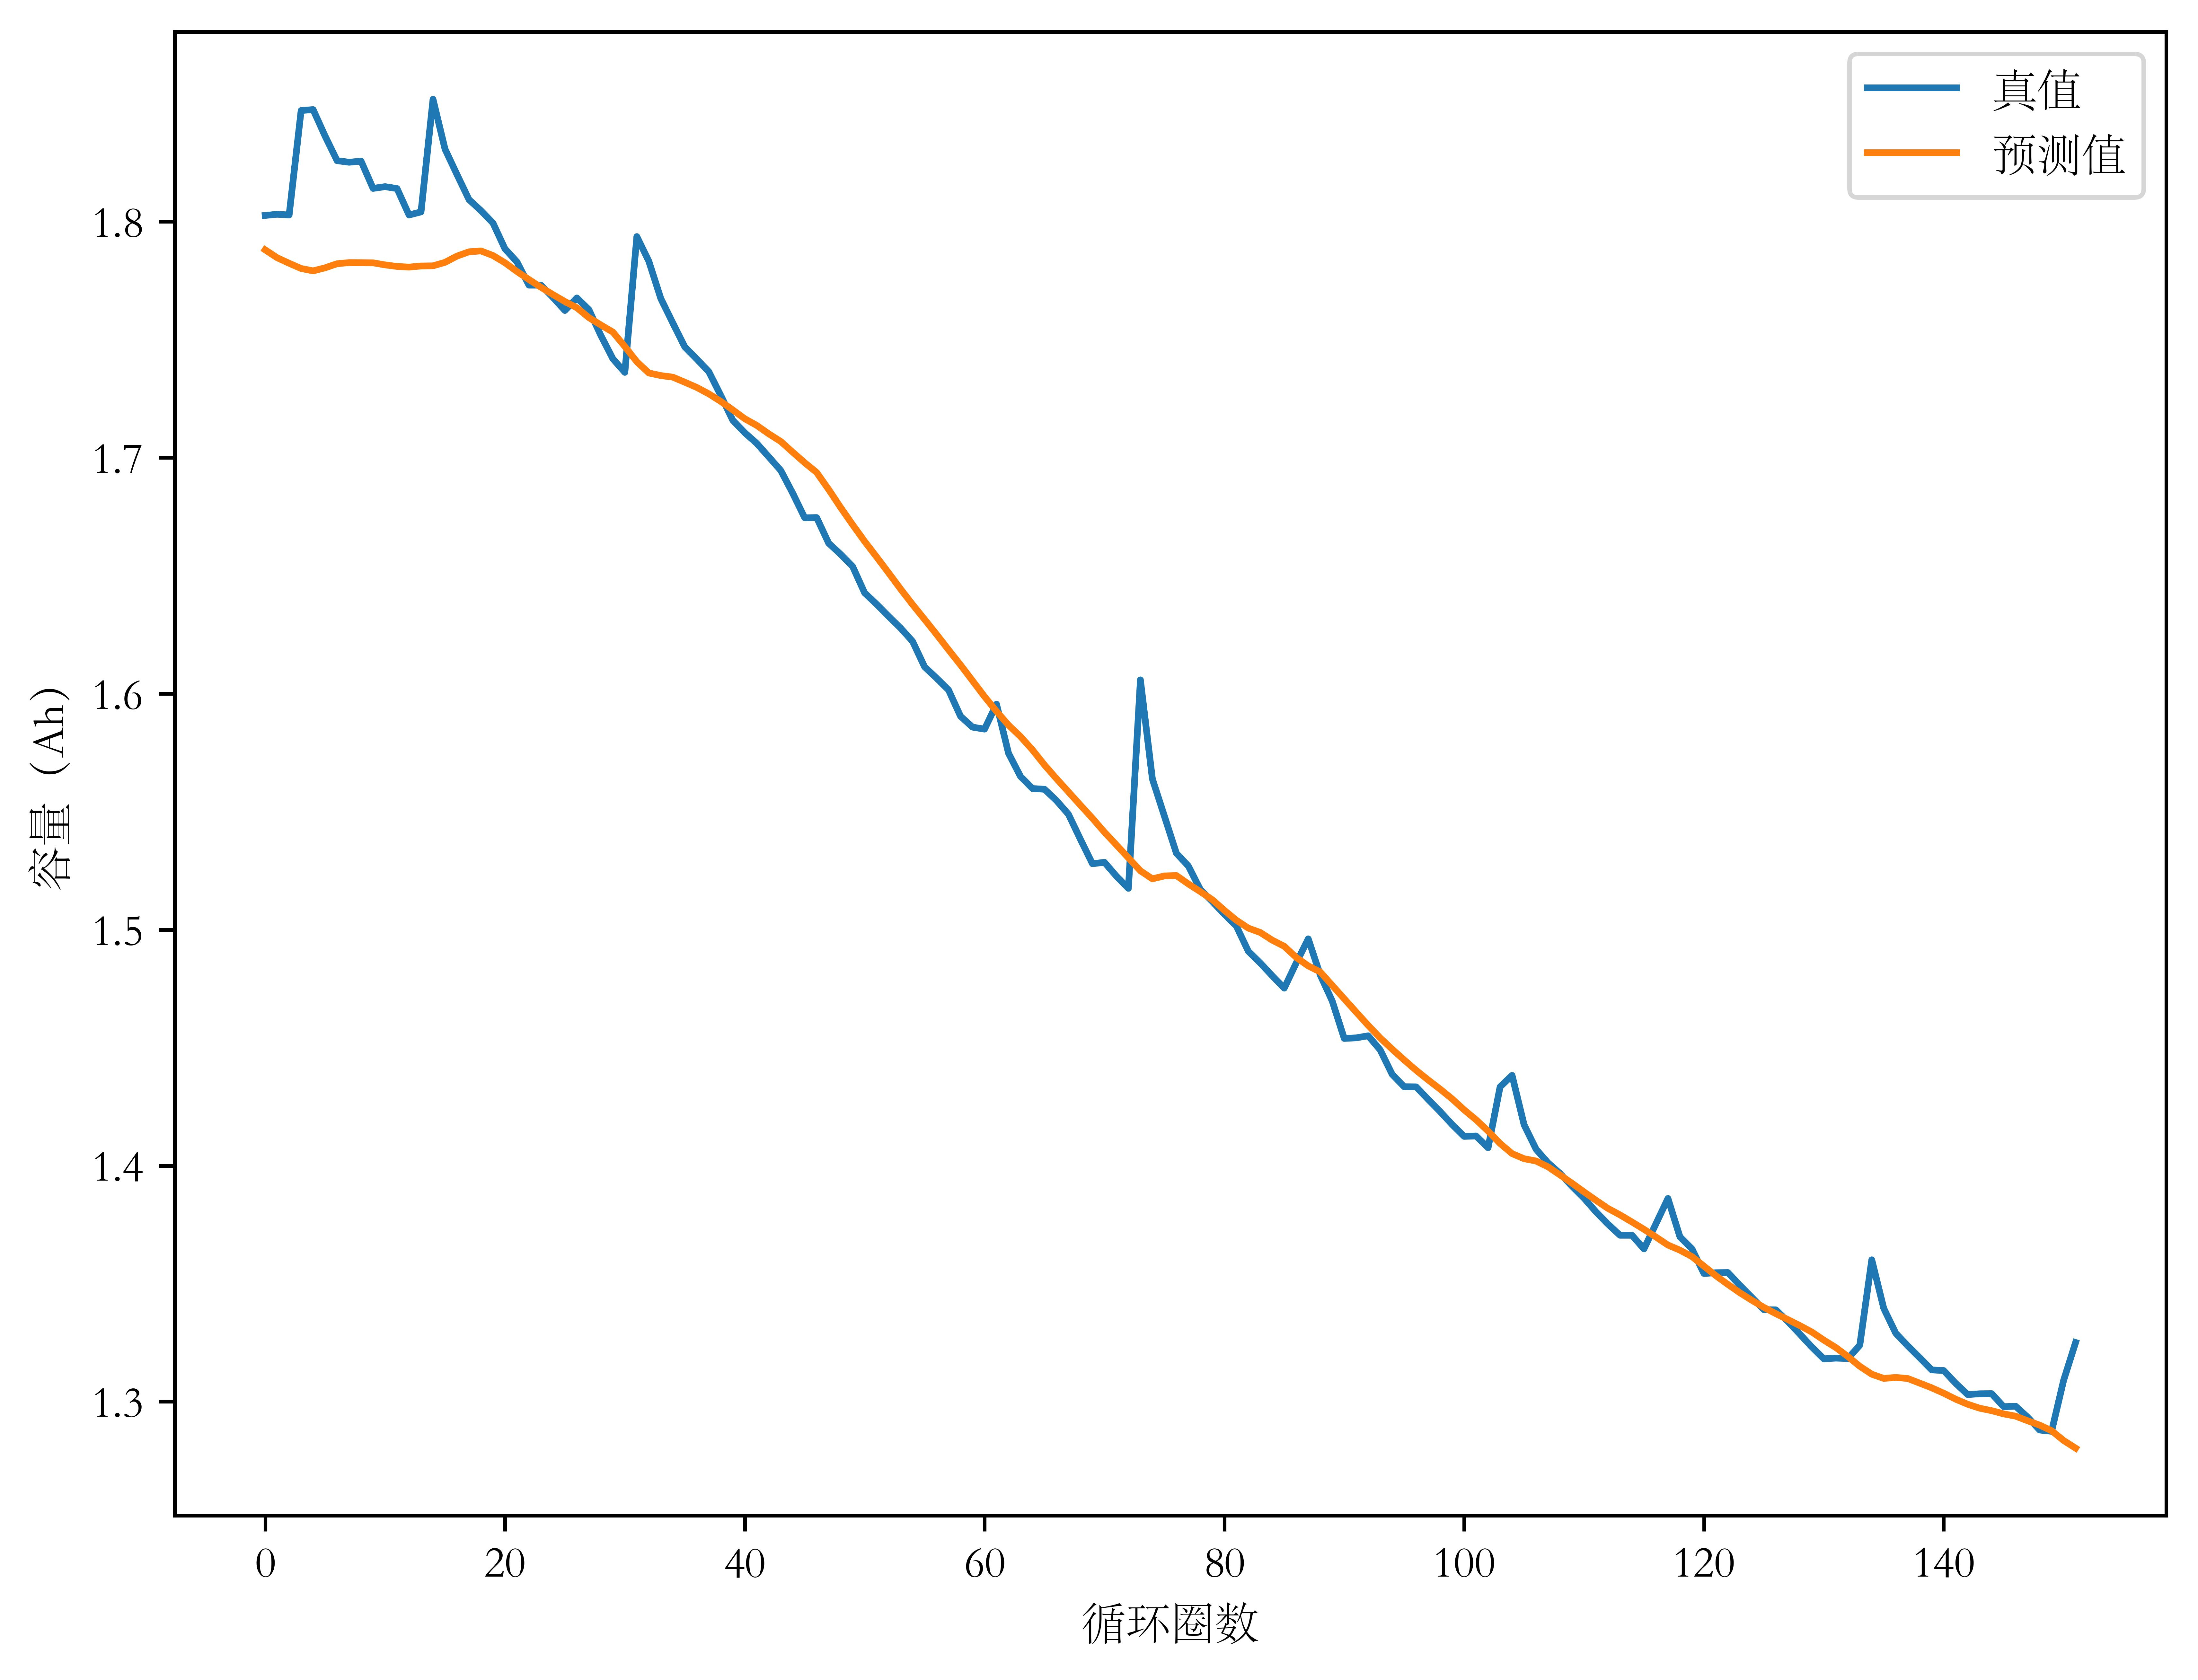
\includegraphics[width=0.15\textwidth]{figures/soh_cap/nasa_B0005_cnn.jpg}}
	\end{figure}
	\begin{figure}[htbp]
		\centering
			{\label{fig:subfig1}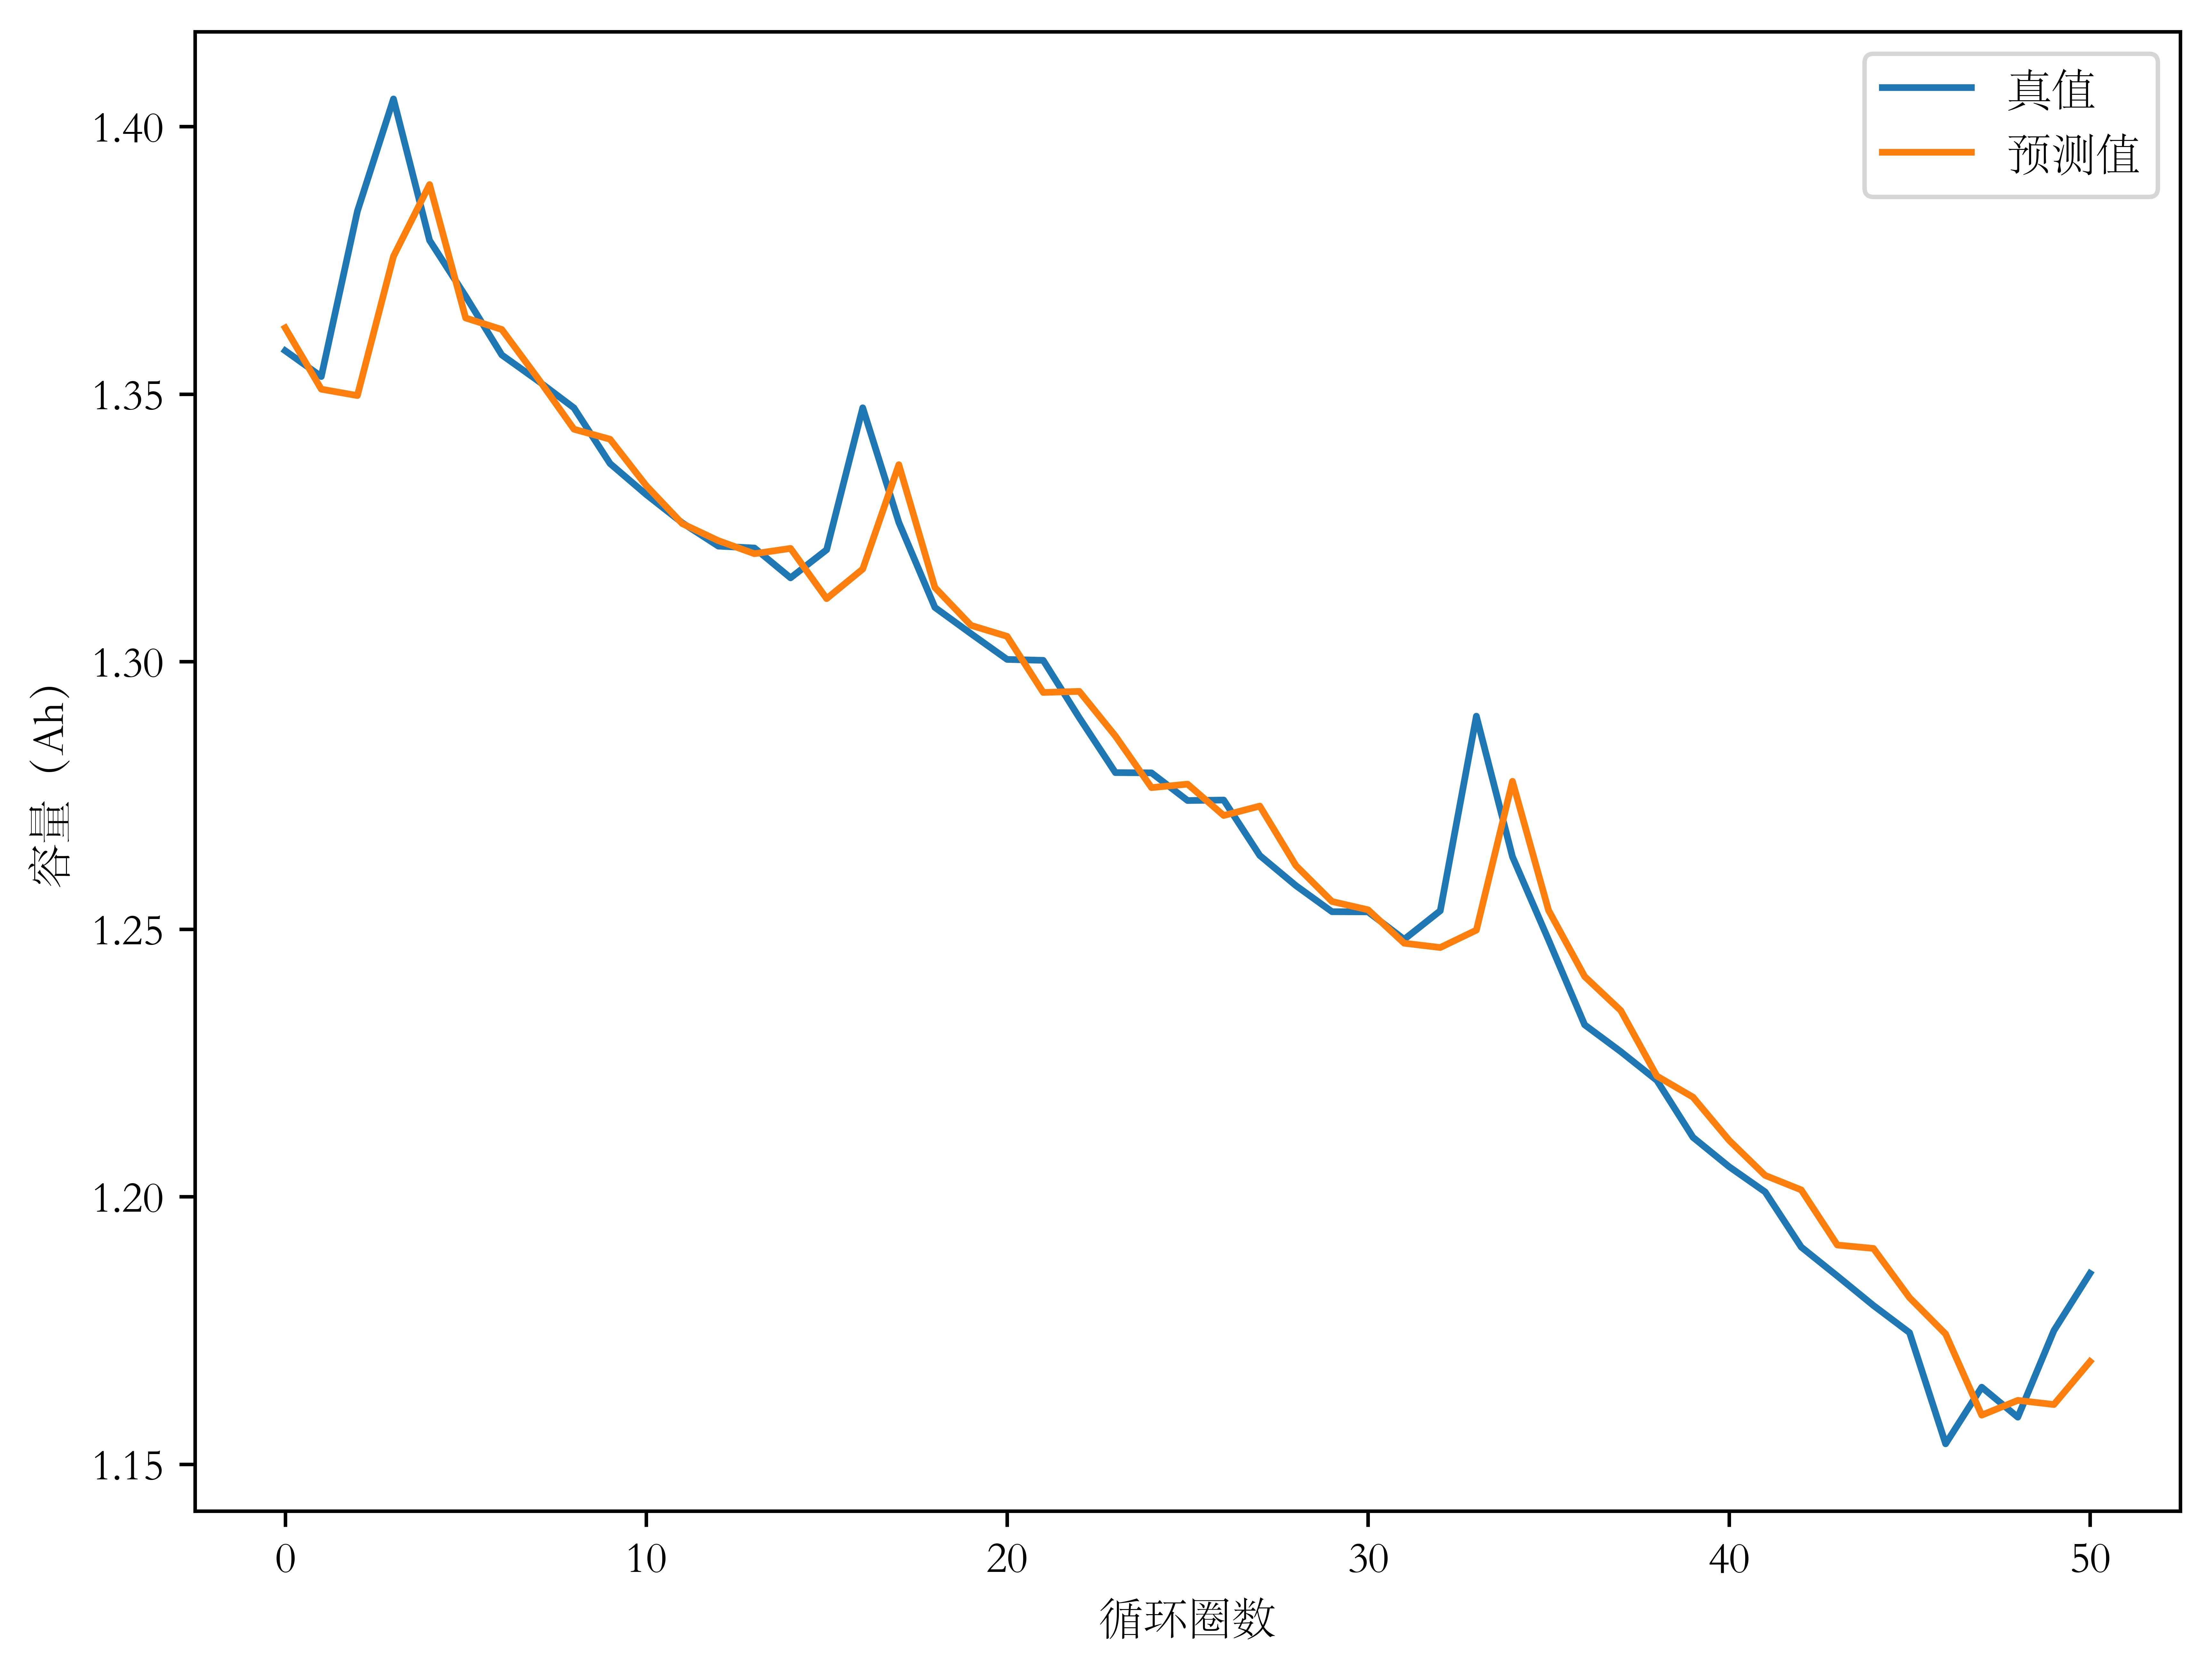
\includegraphics[width=0.15\textwidth]{figures/soh_cap/nasa_B0006_ar.jpg}}
			{\label{fig:subfig2}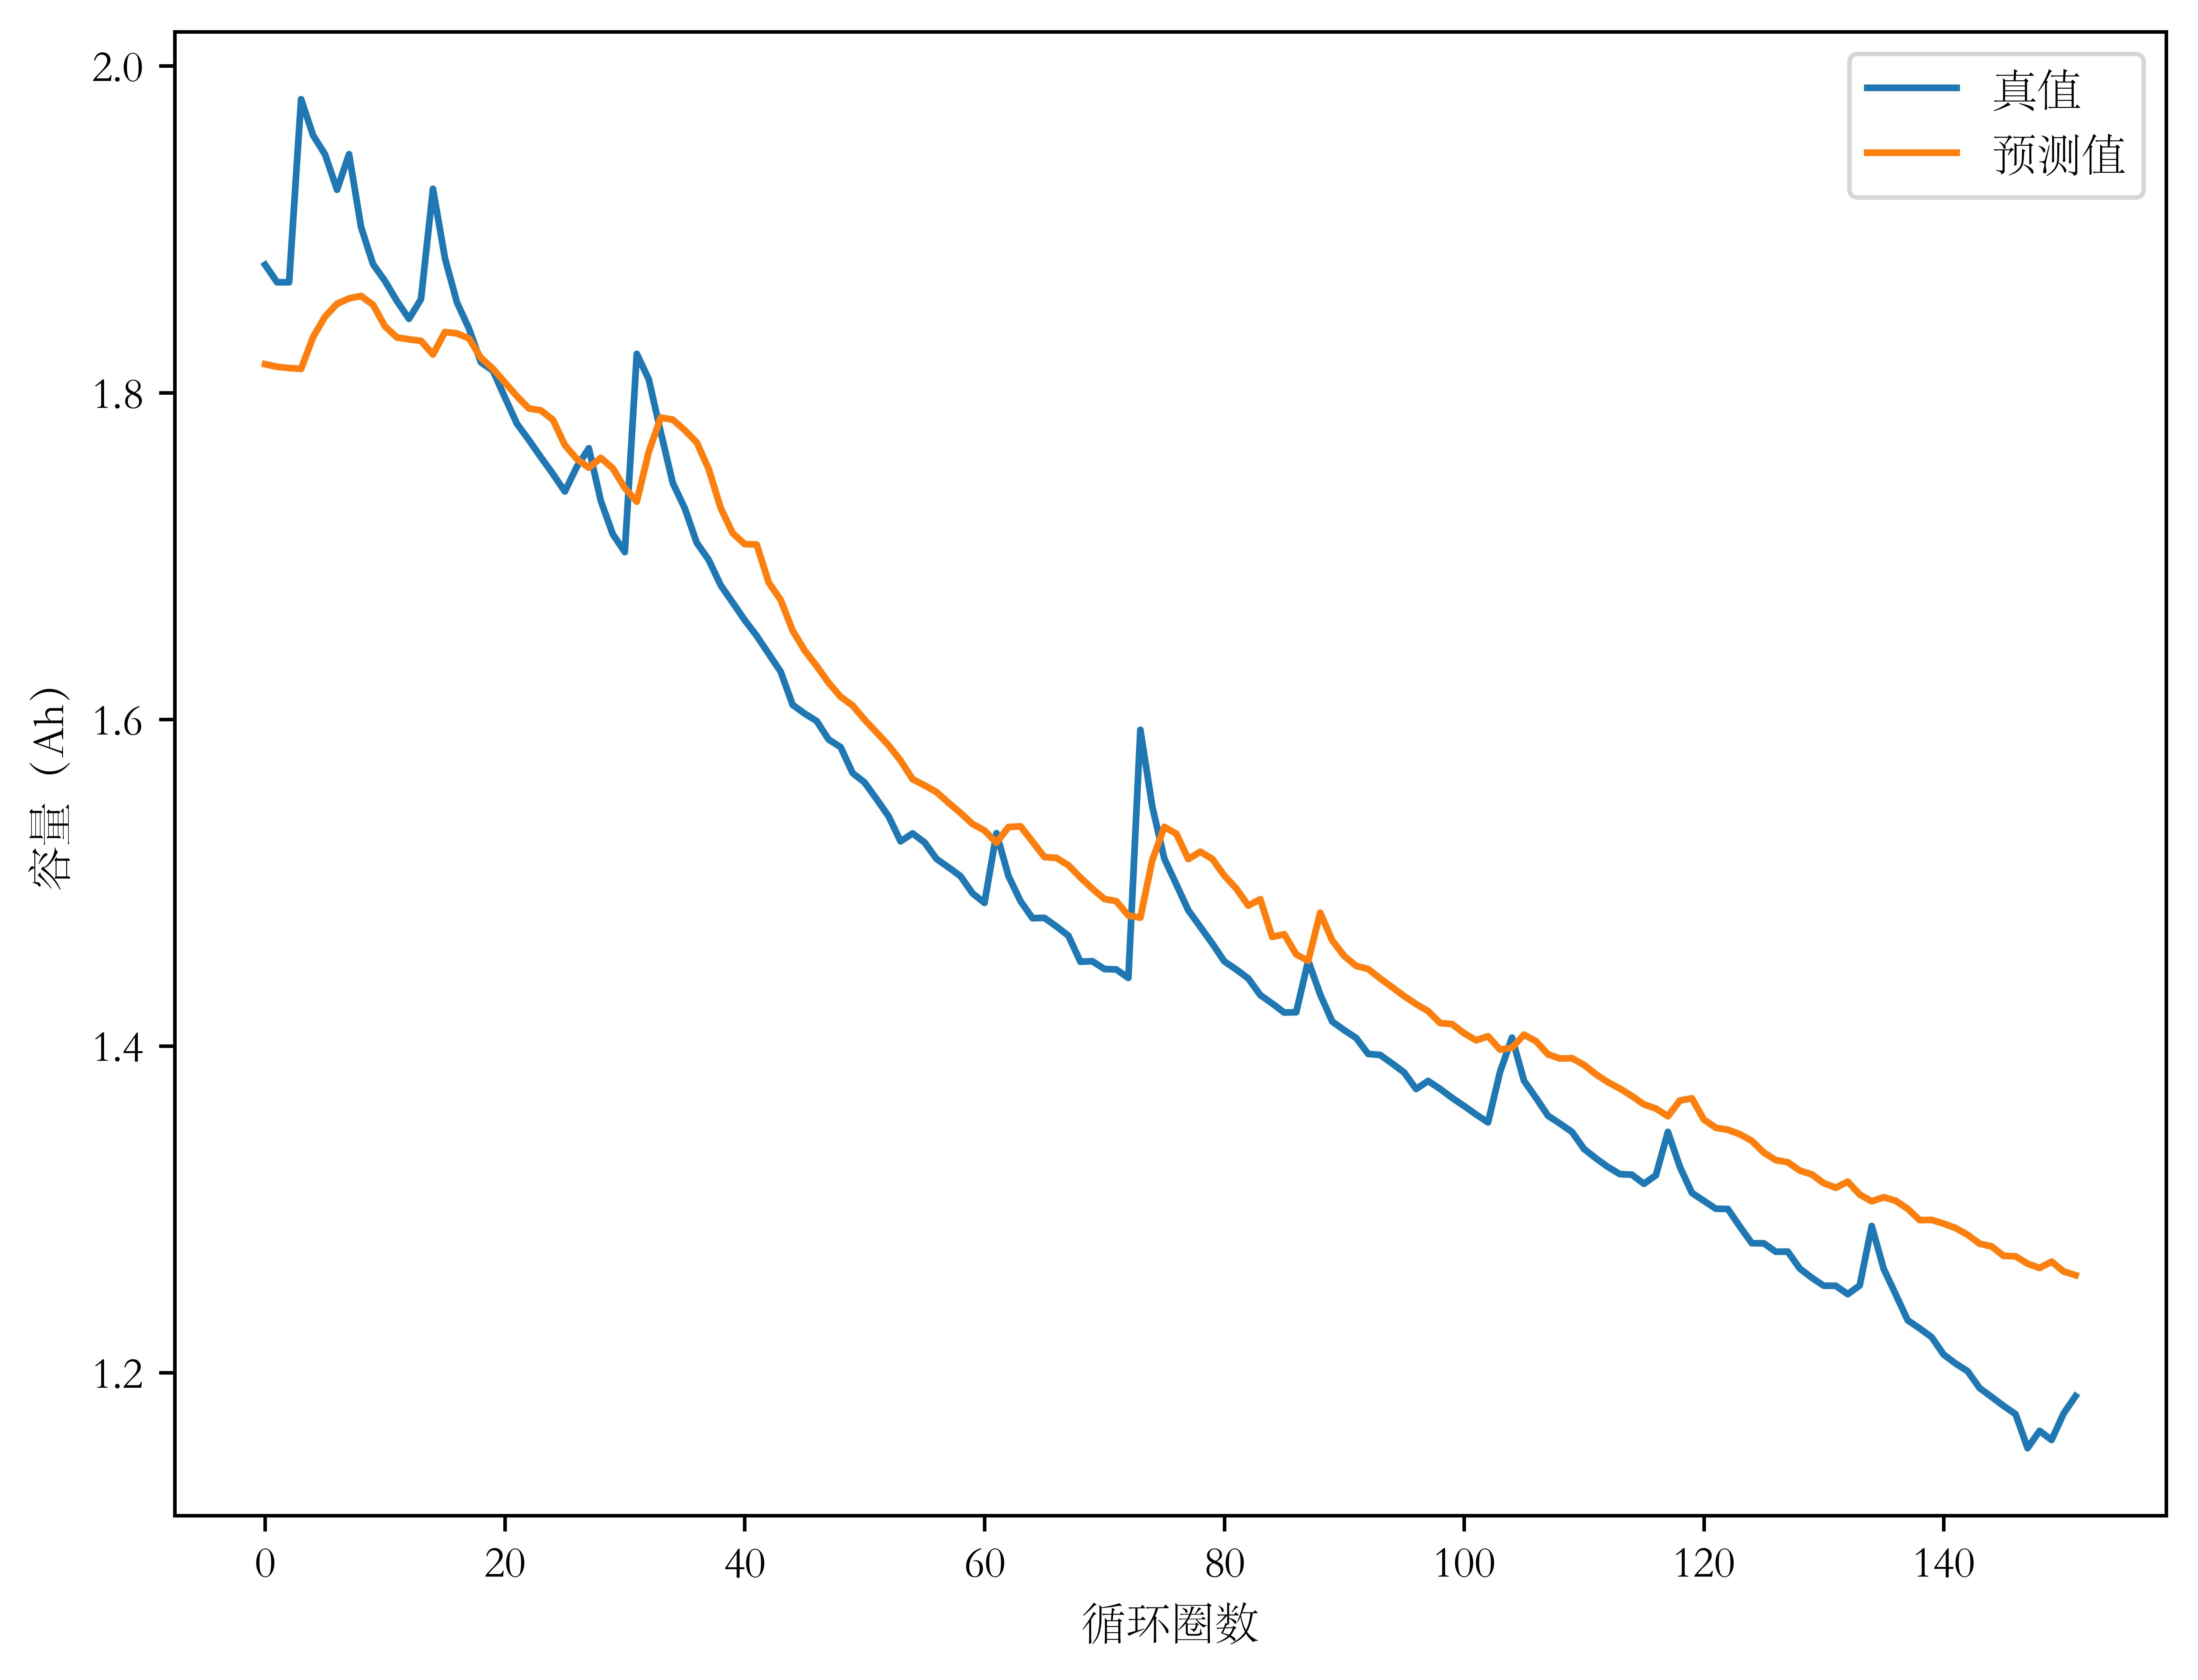
\includegraphics[width=0.15\textwidth]{figures/soh_cap/nasa_B0006_svr.jpg}}
			{\label{fig:subfig3}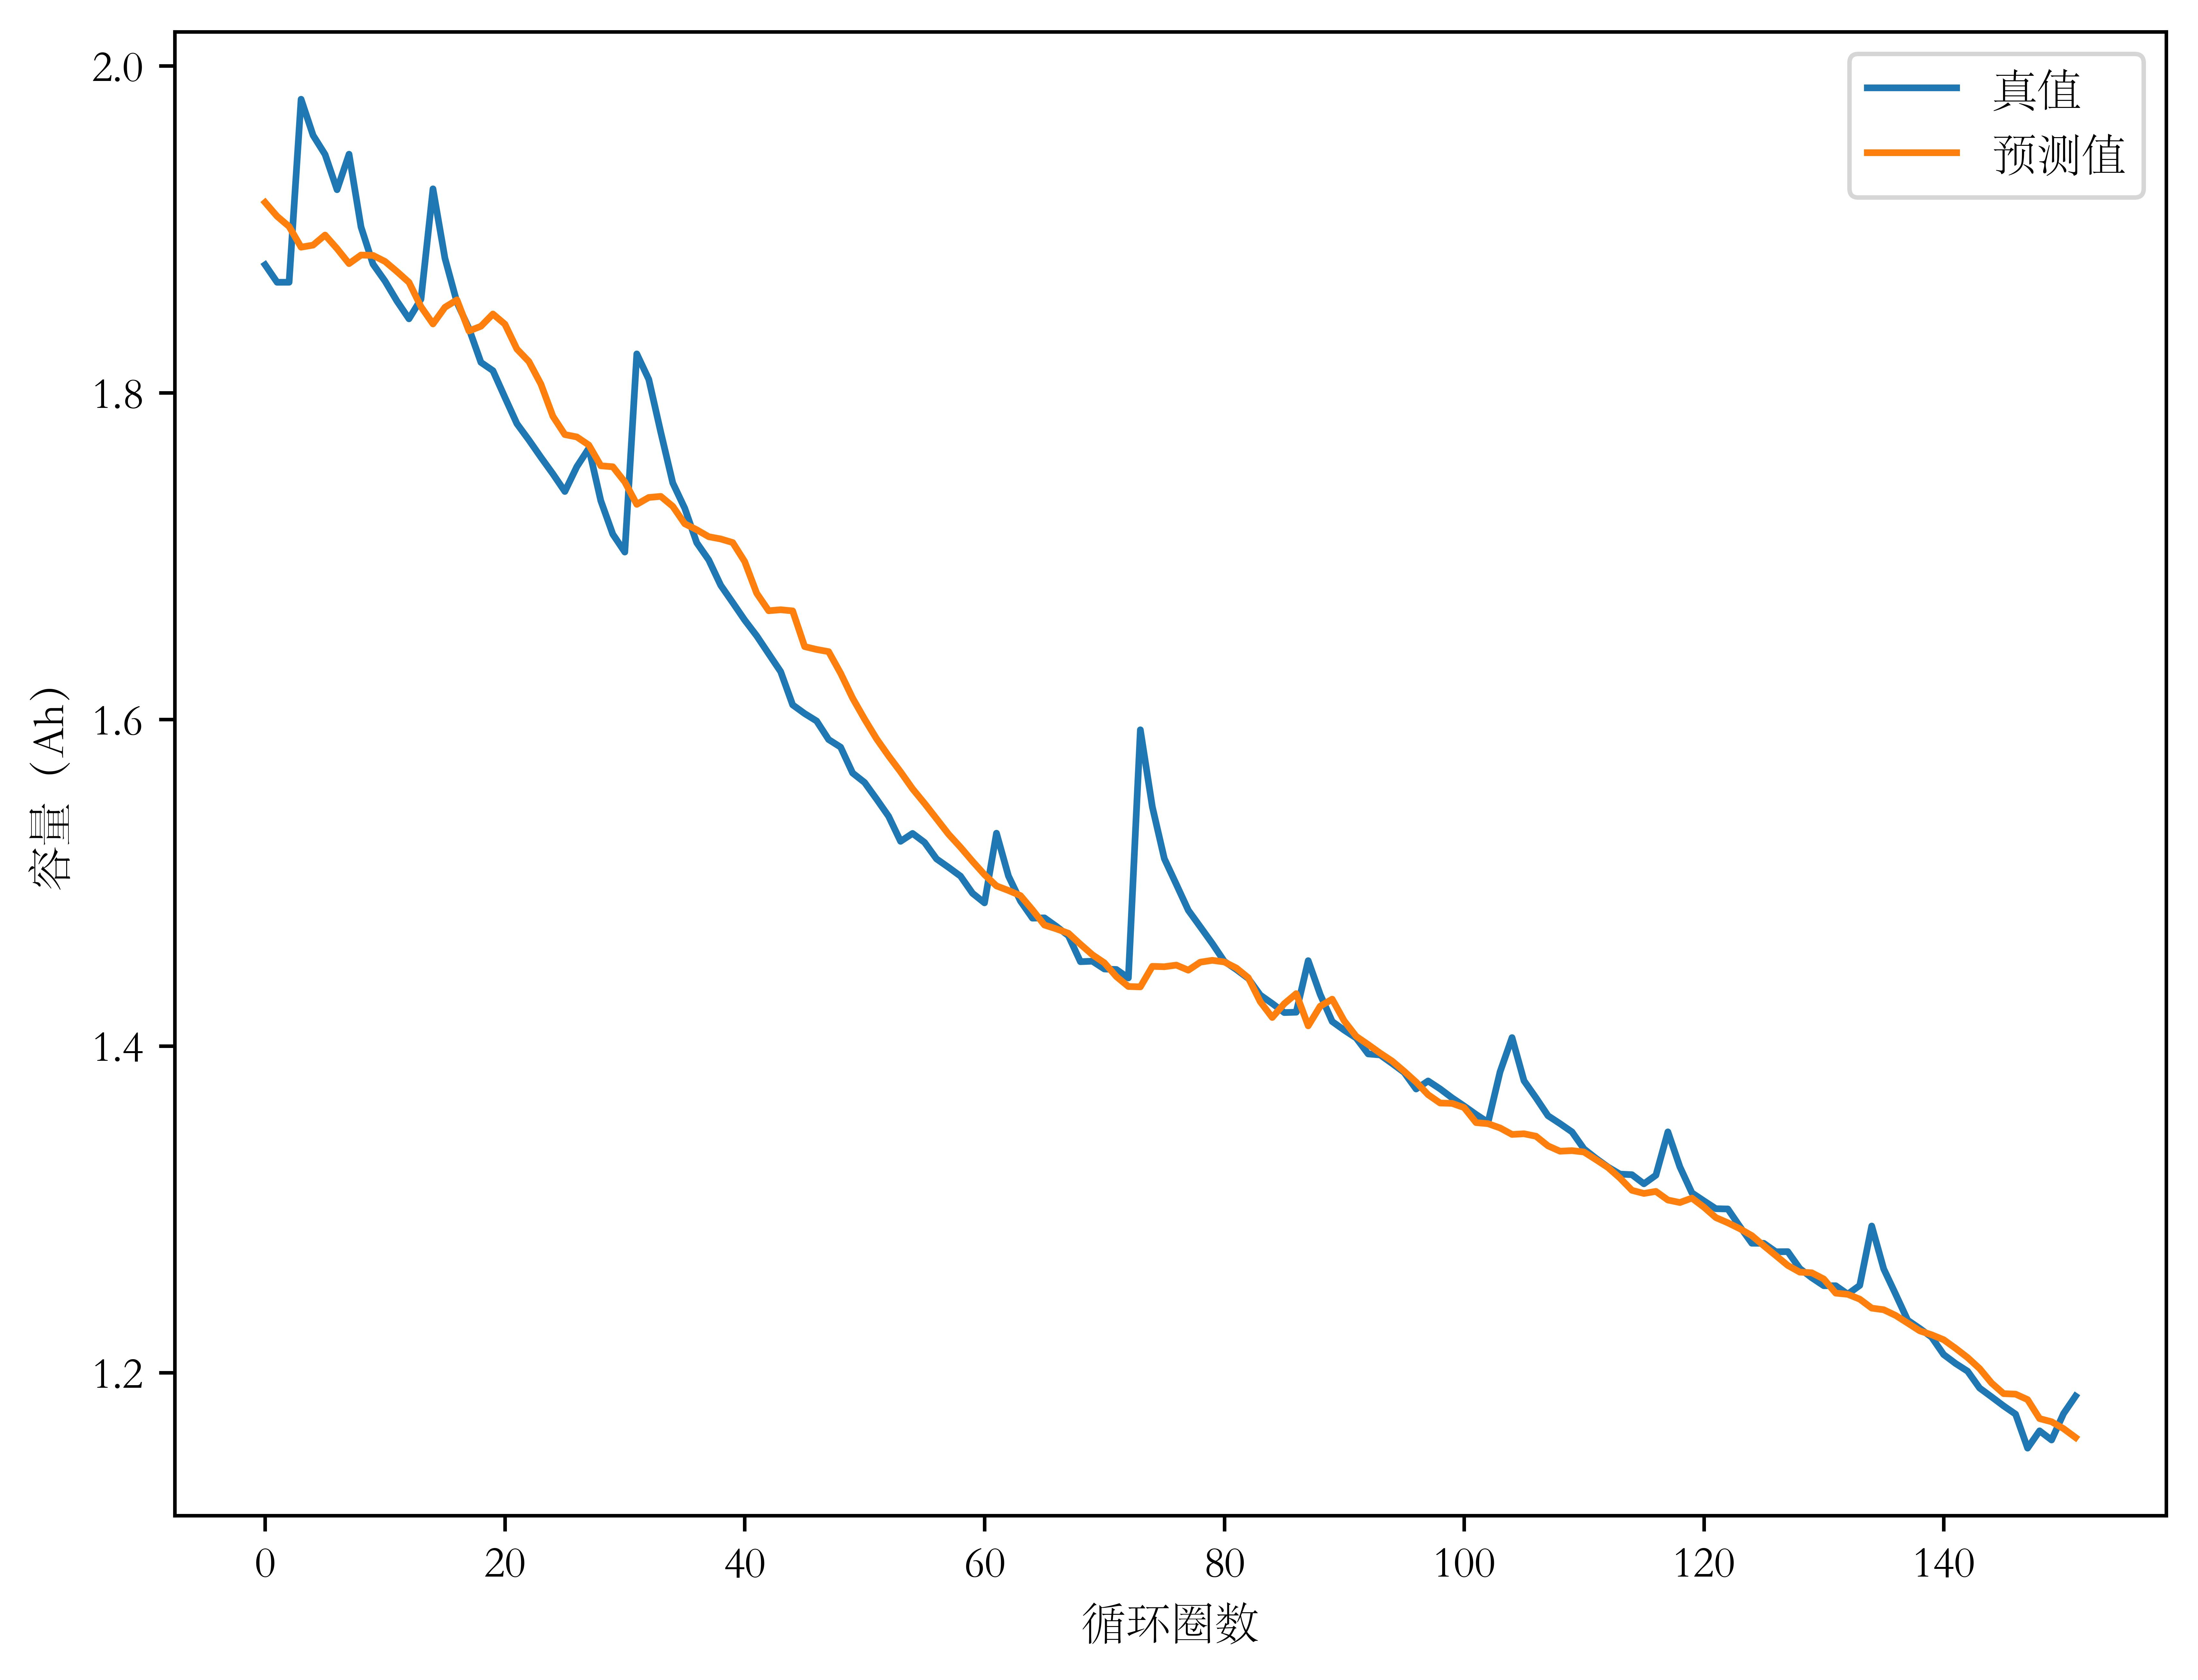
\includegraphics[width=0.15\textwidth]{figures/soh_cap/nasa_B0006_mlp.jpg}}
			{\label{fig:subfig4}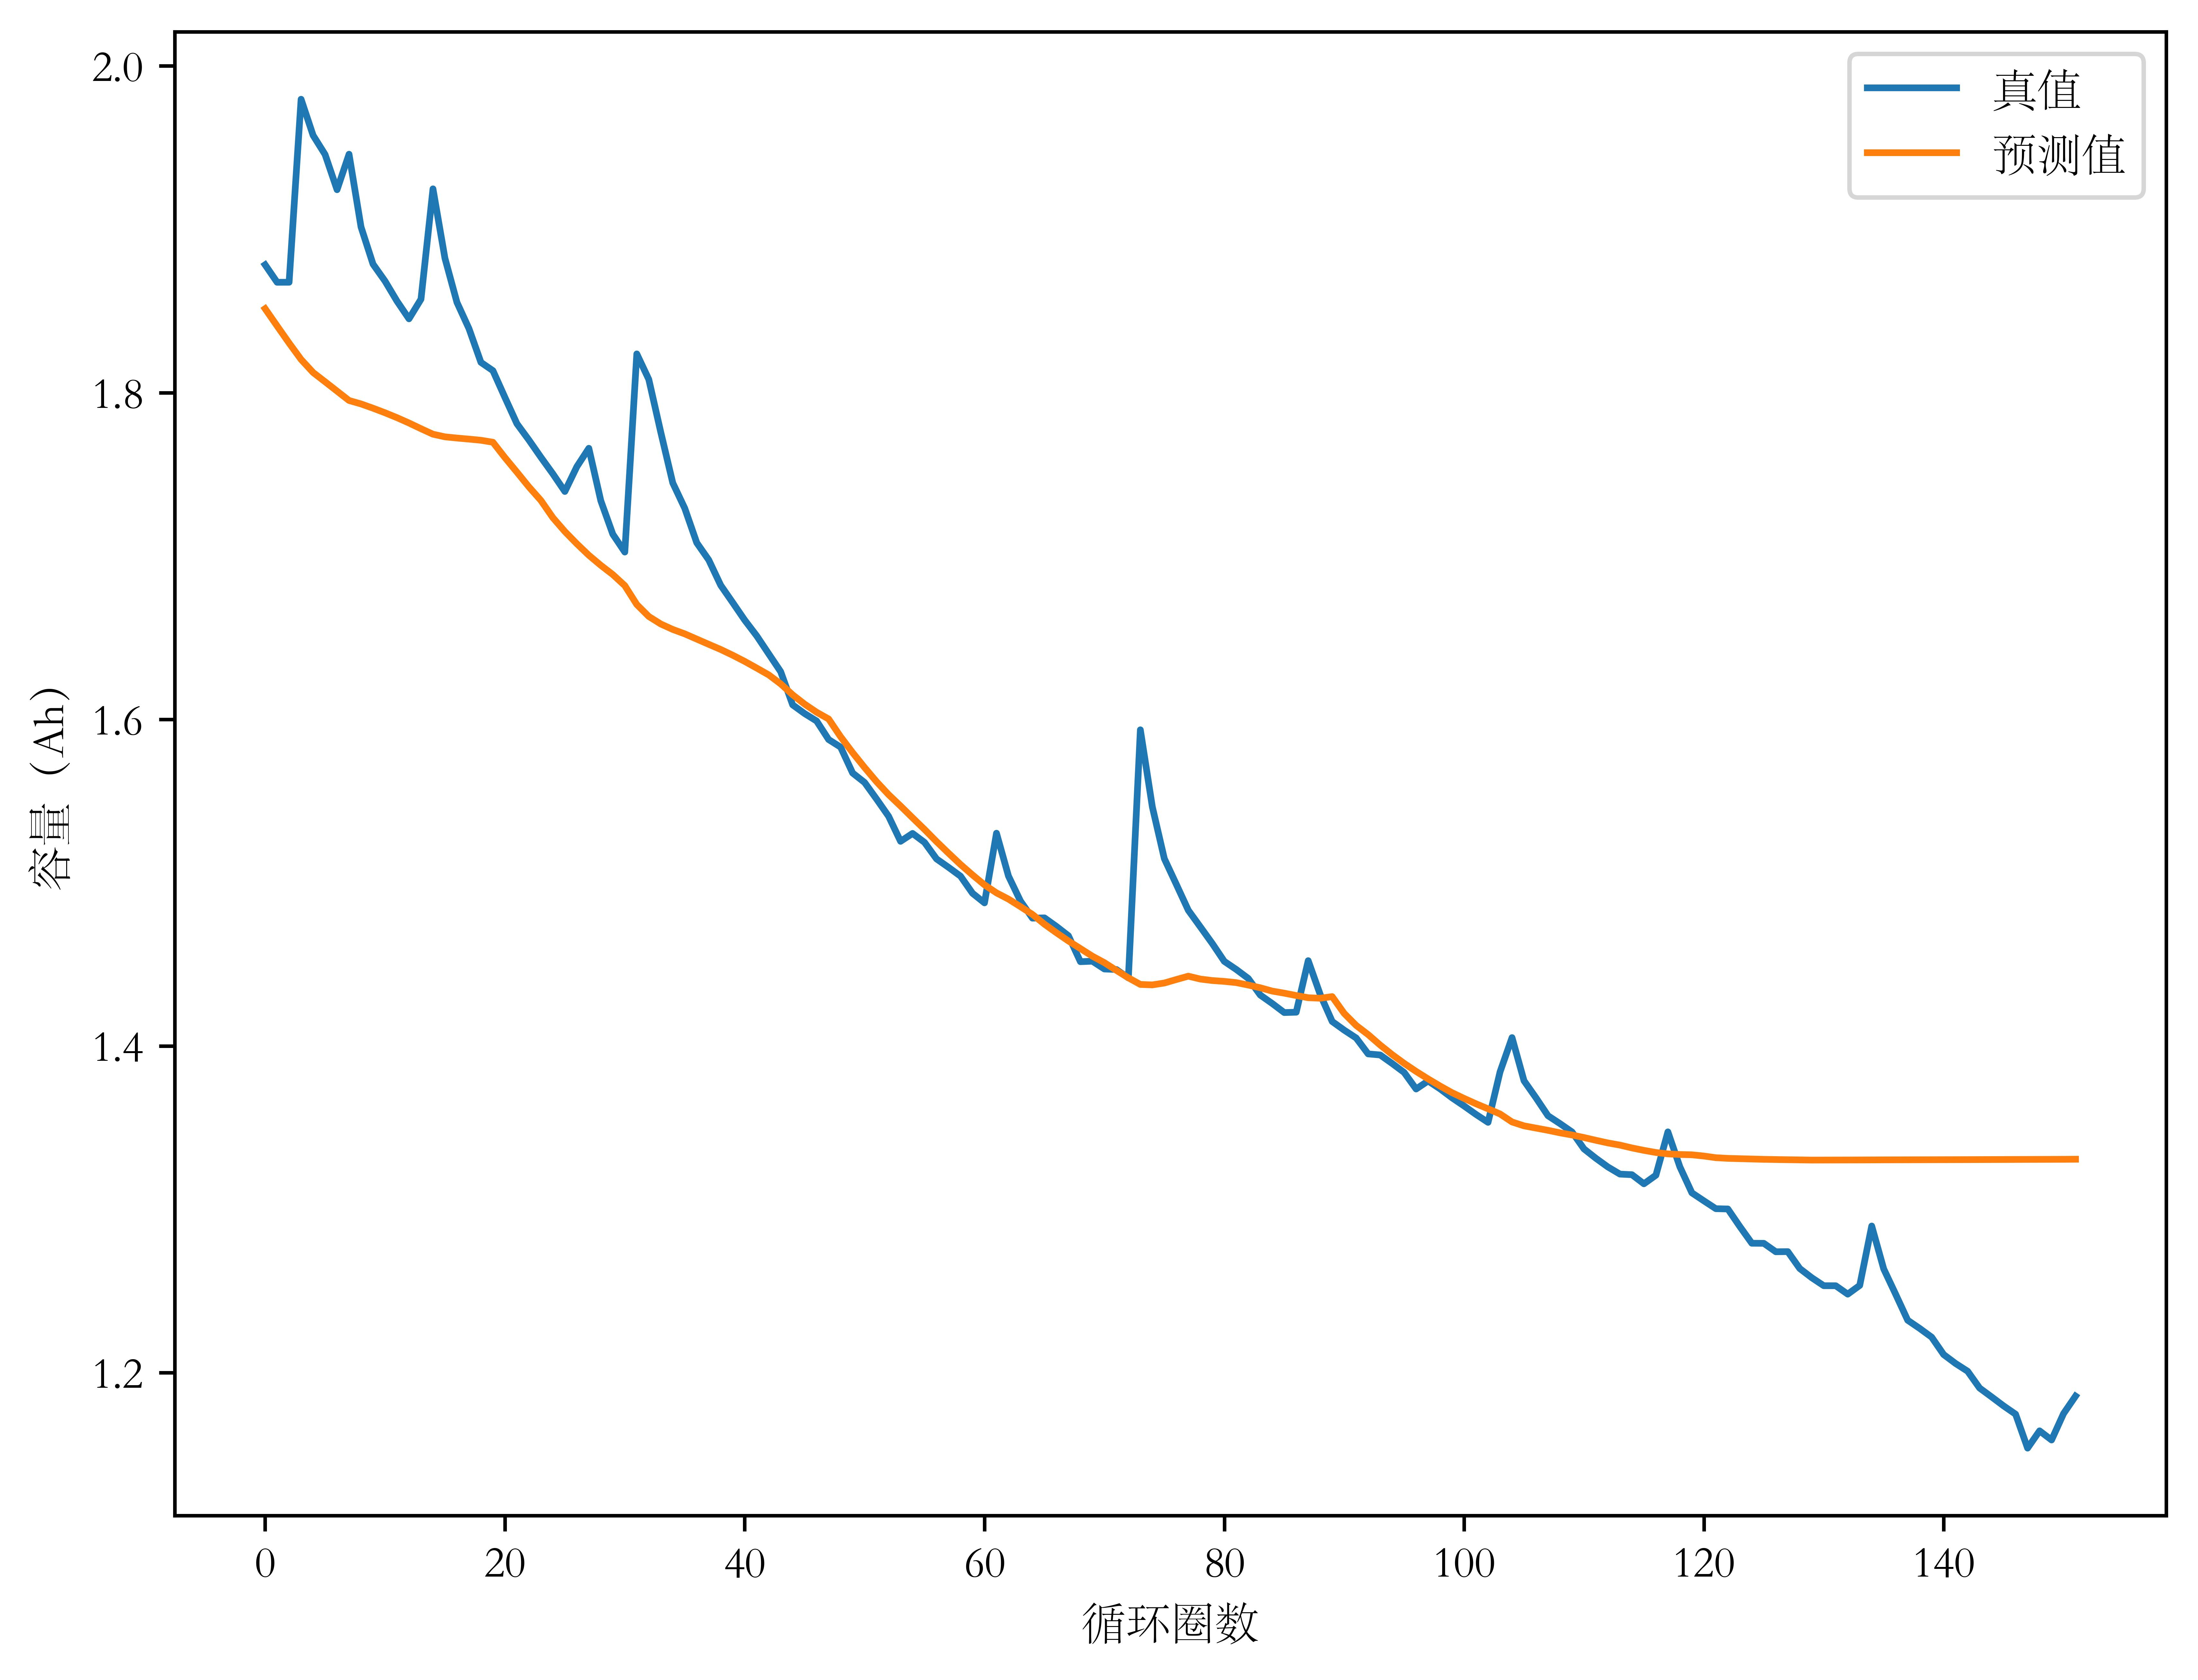
\includegraphics[width=0.15\textwidth]{figures/soh_cap/nasa_B0006_lstm.jpg}}
			{\label{fig:subfig5}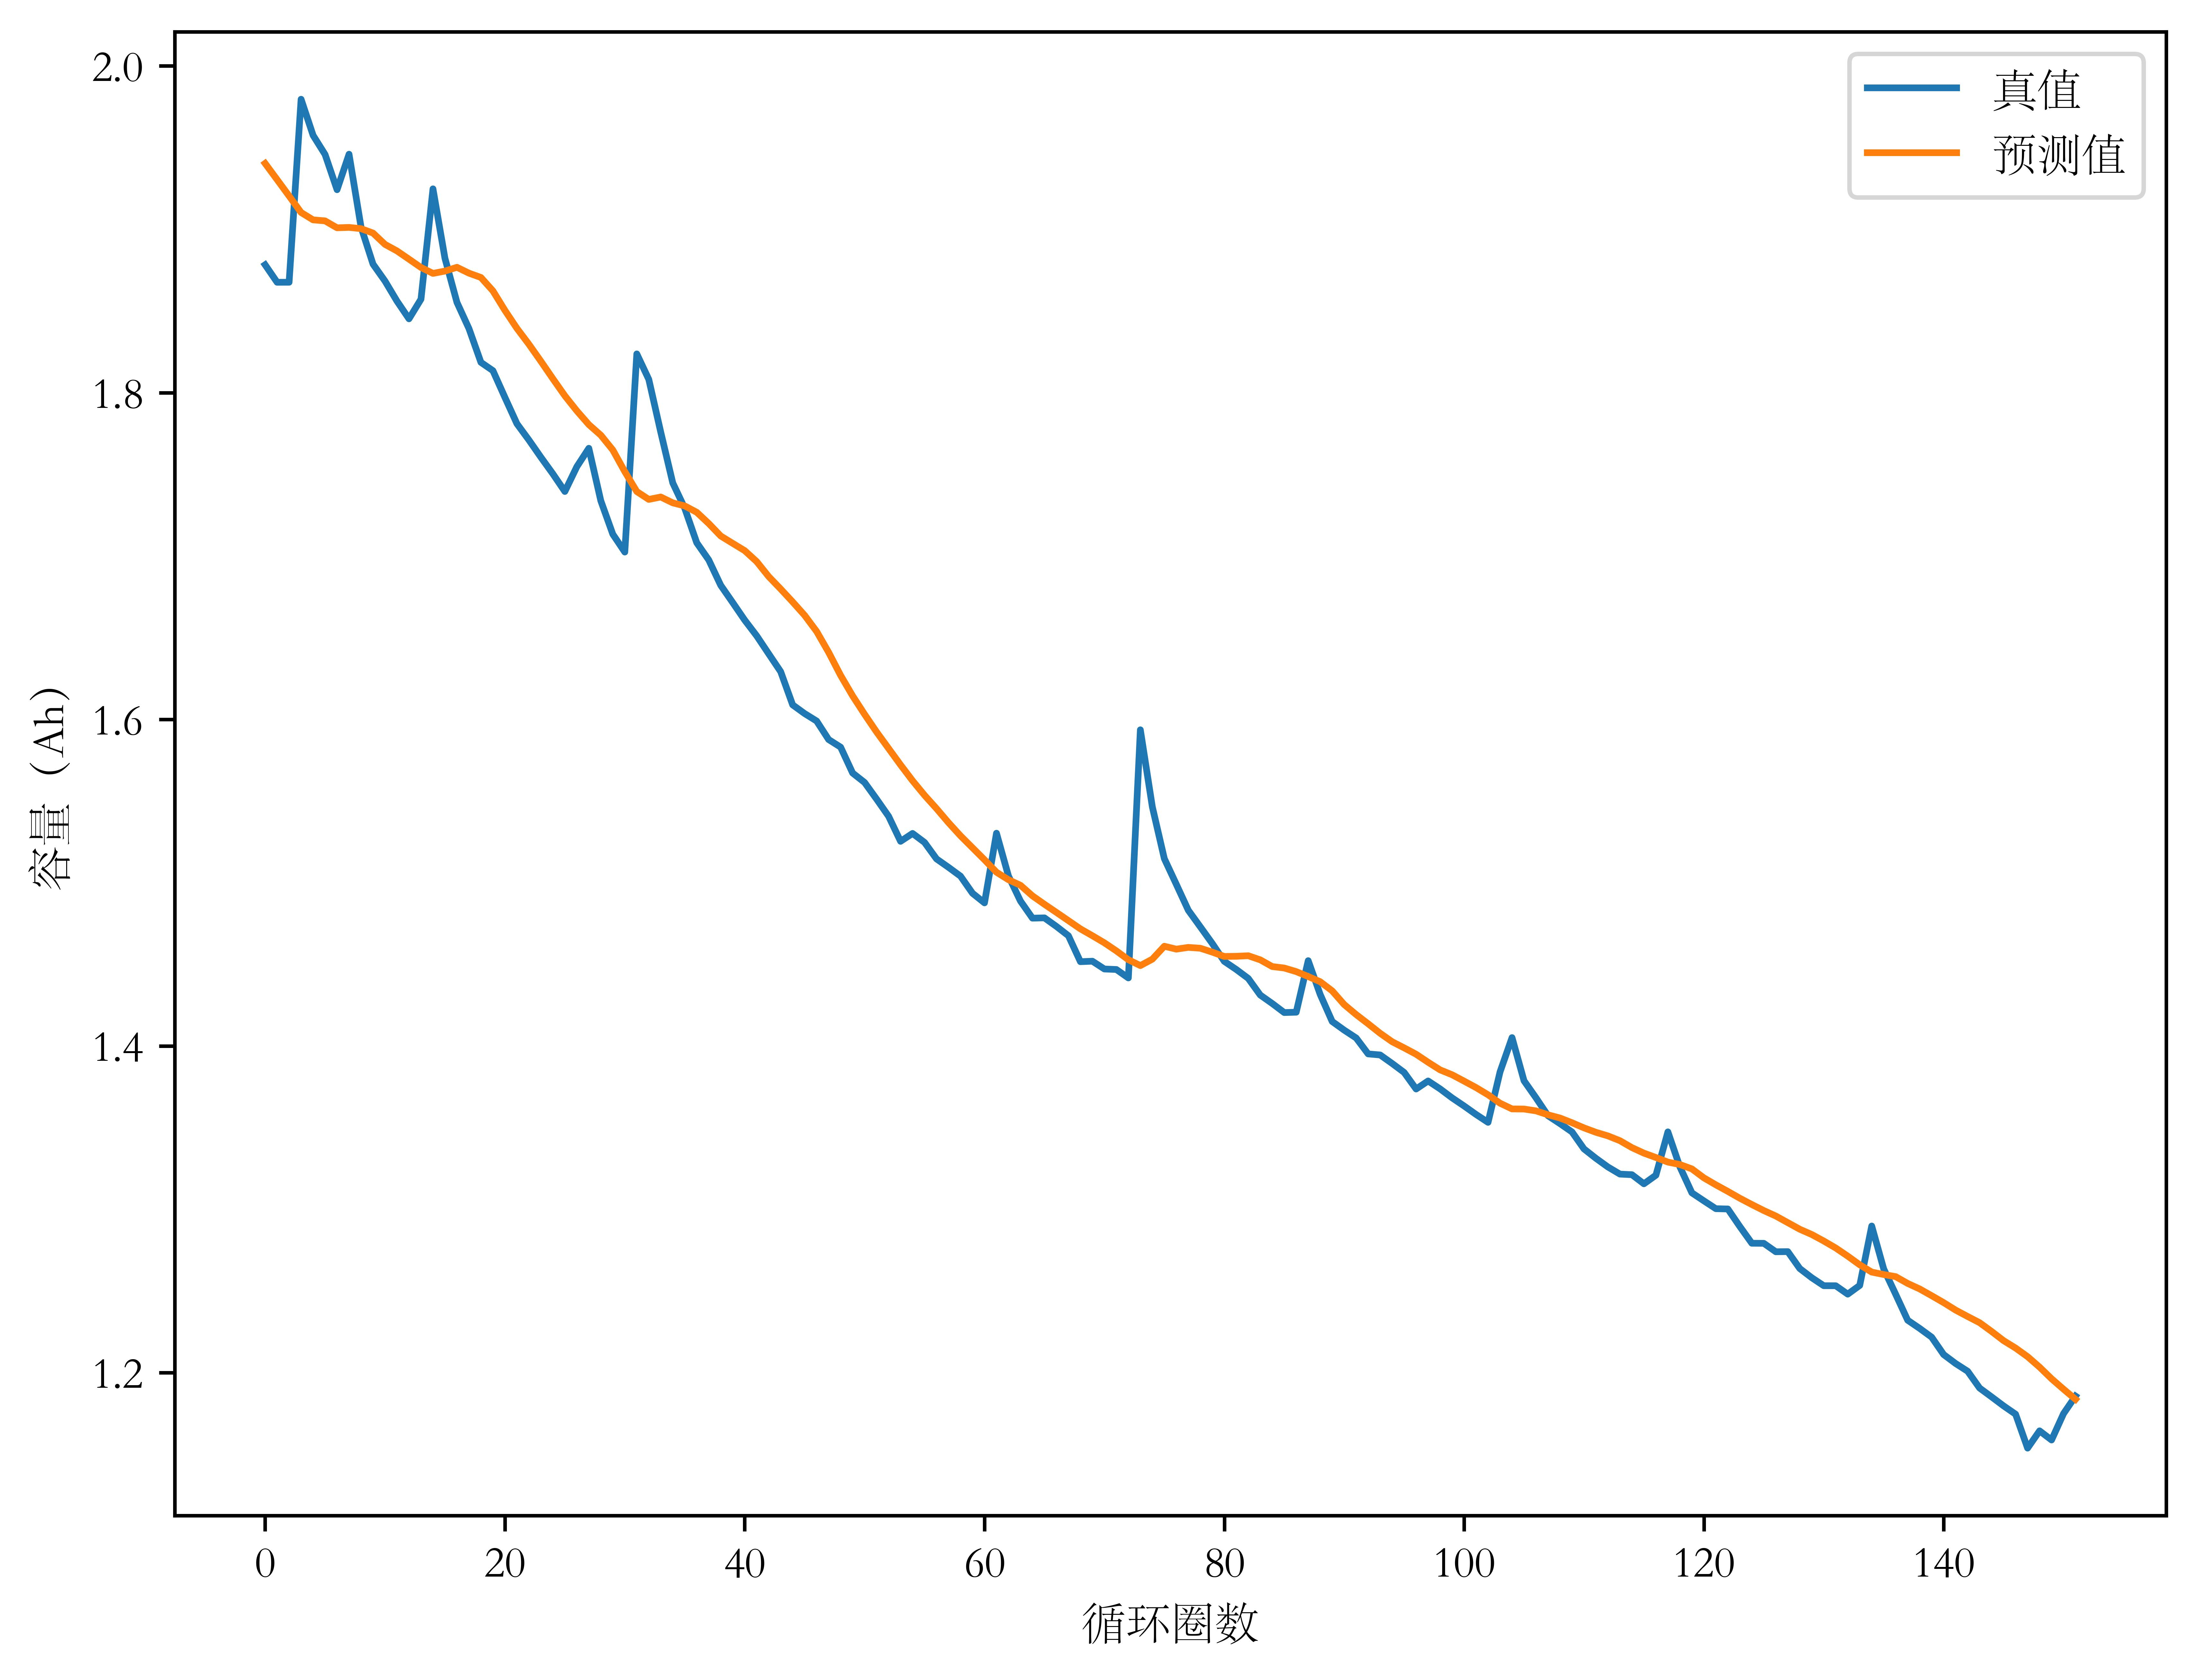
\includegraphics[width=0.15\textwidth]{figures/soh_cap/nasa_B0006_cnn.jpg}}
	\end{figure}
\end{frame}

\begin{frame}
\begin{table}[]
	\centering
	\resizebox{\columnwidth}{!}{%
	\begin{tabular}{ccccccccccc}
	\toprule
	\multirow{2}{*}{指标} & \multicolumn{5}{l}{CALCE数据集}          & \multicolumn{5}{l}{NASA PCoE数据集}      \\
						& AR    & SVR   & MLP   & LSTM  & CNN   & AR    & SVR   & MLP   & LSTM  & CNN   \\
	\midrule
	平均MaxE              & 0.116 & 0.141 & 0.147 & 0.152 & 0.142 & 0.054 & 0.097 & 0.111 & 0.158 & 0.113 \\
	平均MAE               & 0.010 & 0.023 & 0.009 & 0.028 & 0.008 & 0.008 & 0.033 & 0.019 & 0.041 & 0.020 \\
	平均RMSE              & 0.016 & 0.028 & 0.014 & 0.035 & 0.013 & 0.013 & 0.037 & 0.026 & 0.057 & 0.027 \\
	\bottomrule
	\end{tabular}%
	}
	\caption{五种模型预测性能评估结果}
	\end{table}
	\begin{itemize}
		\item 五个模型均取得较高预测精度,使用数据驱动方法实现锂离子电池SOH估计具有可行性
		\item 对于短时预测问题,非隐状态模型的预测精度高于隐状态模型
	\end{itemize}
\end{frame}

\subsection{基于电池充放电直接测量量的SOH估计}

\begin{frame}
	\begin{figure}[htbp]
		\centering
			{\label{fig:subfig1}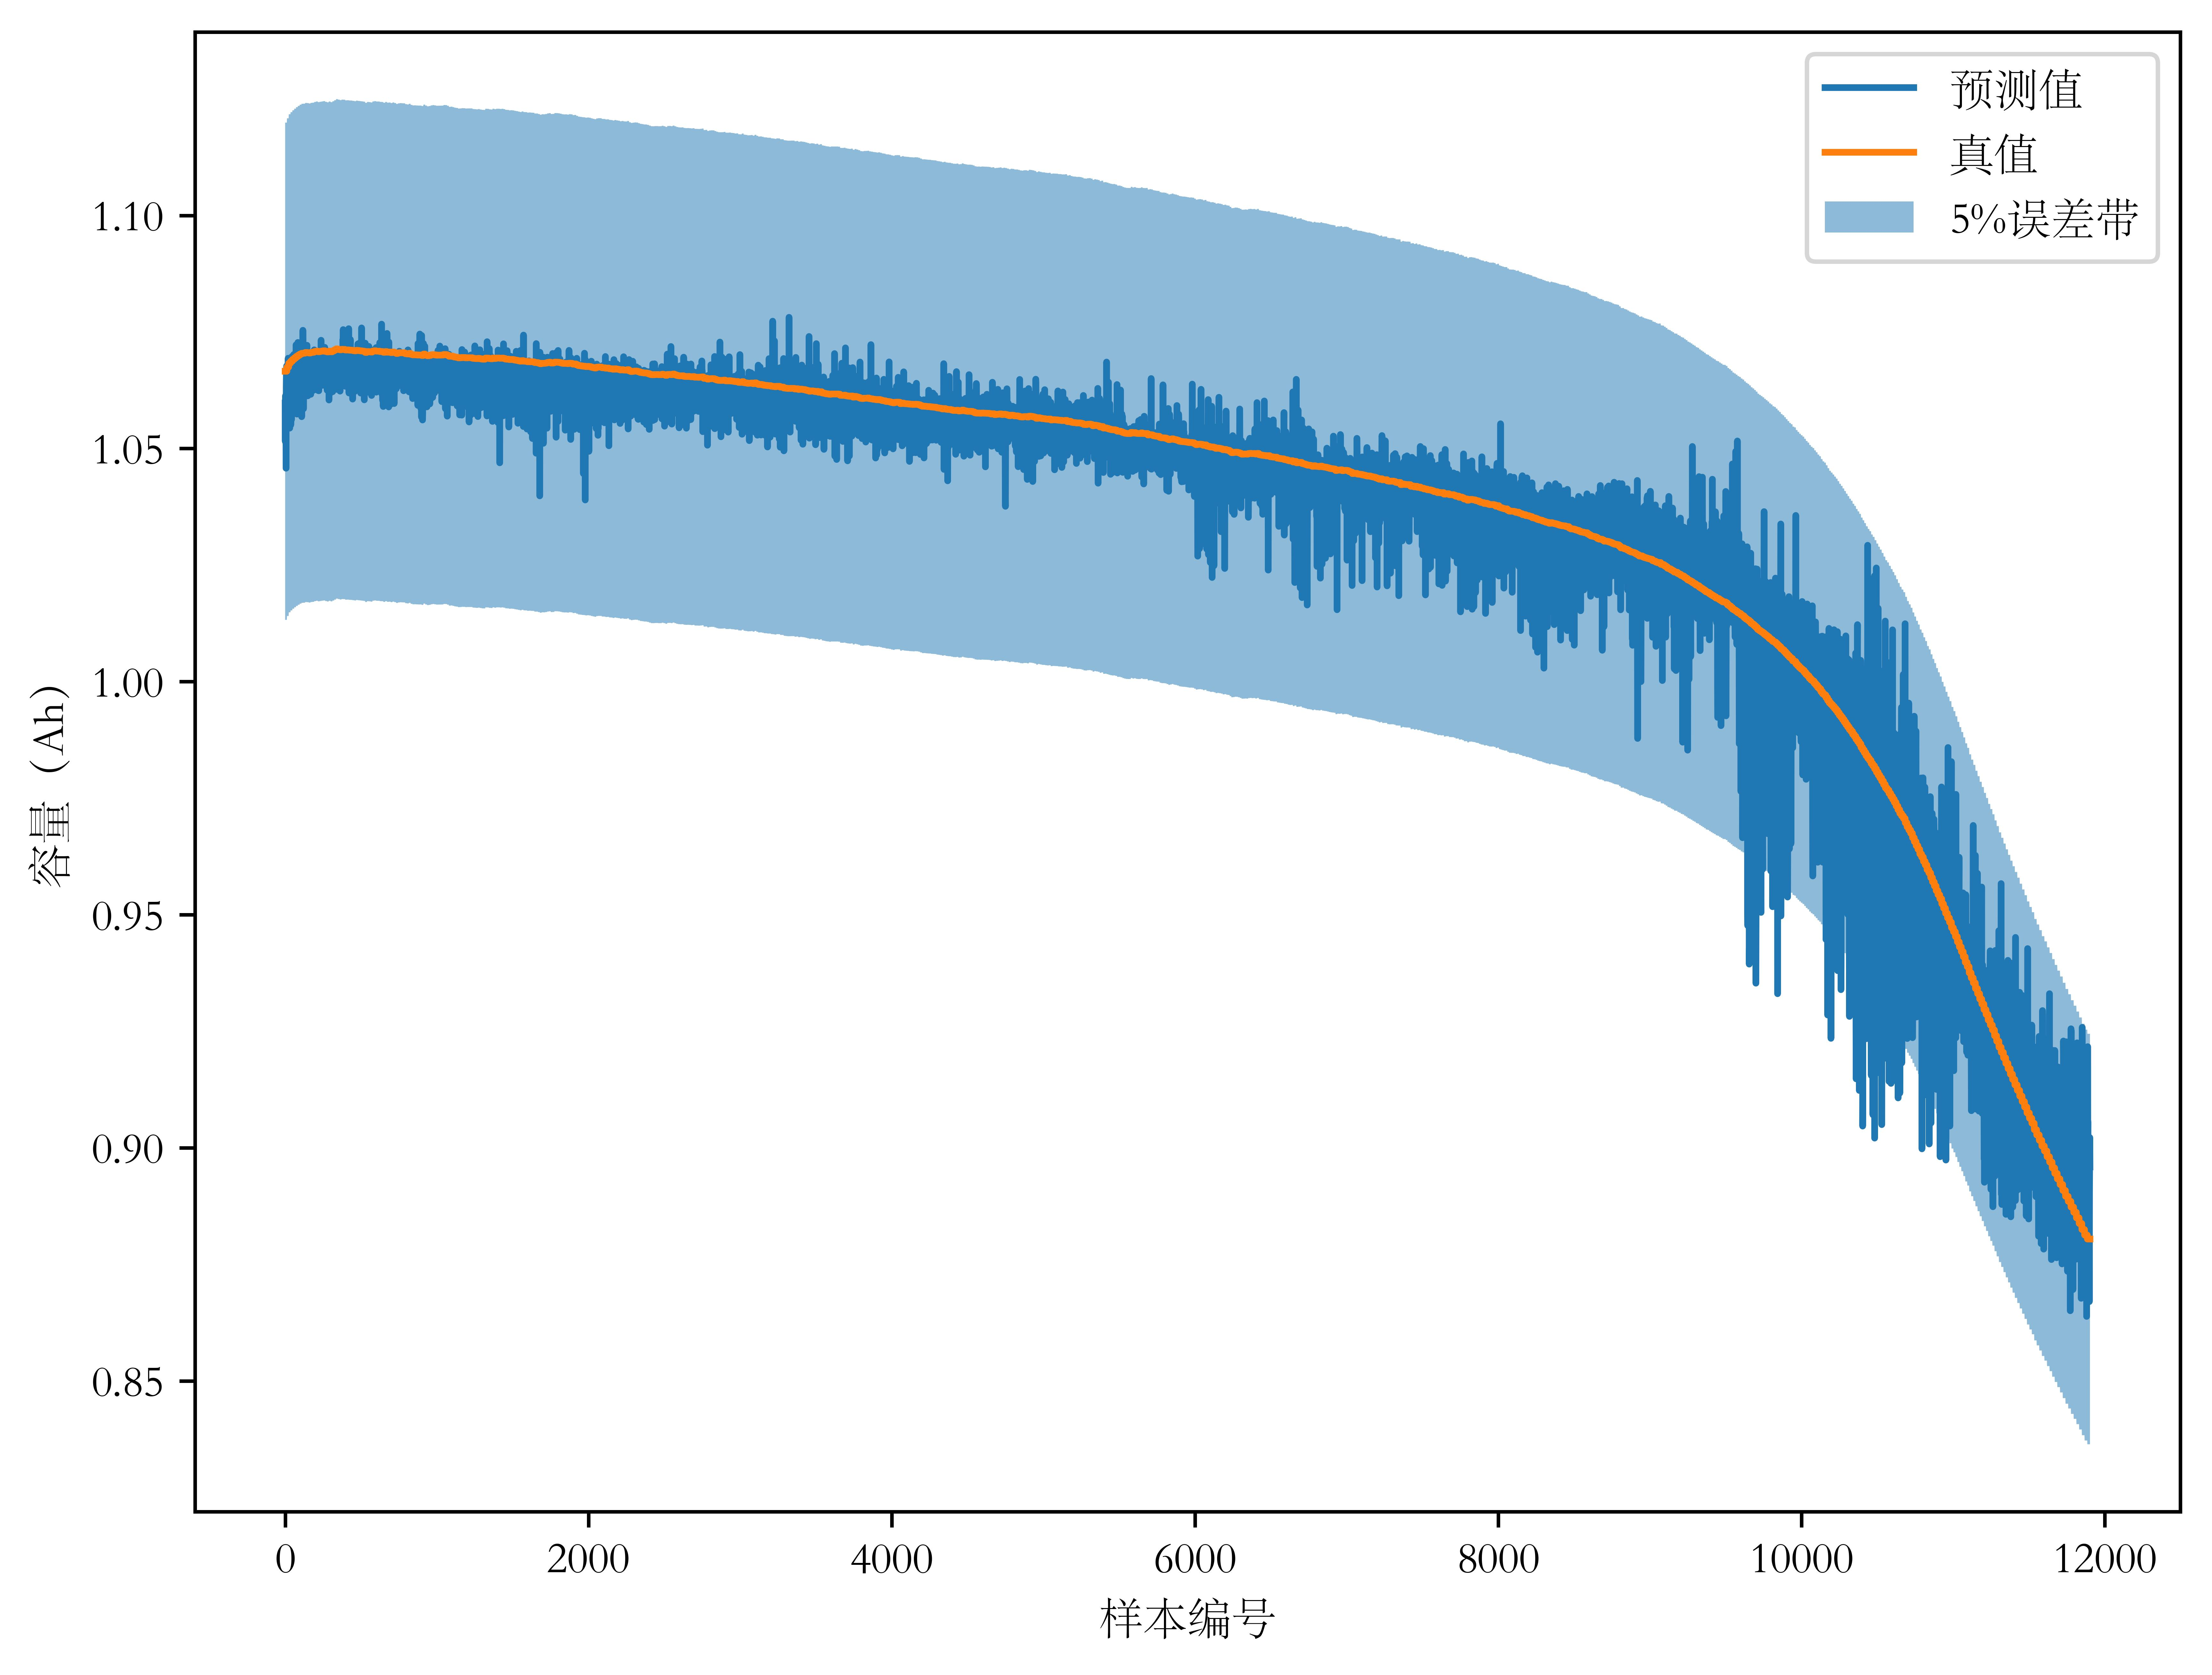
\includegraphics[width=0.2\textwidth]{figures/soh_vitq/tri_group1_cell1_cnn_vit.jpg}}
			{\label{fig:subfig2}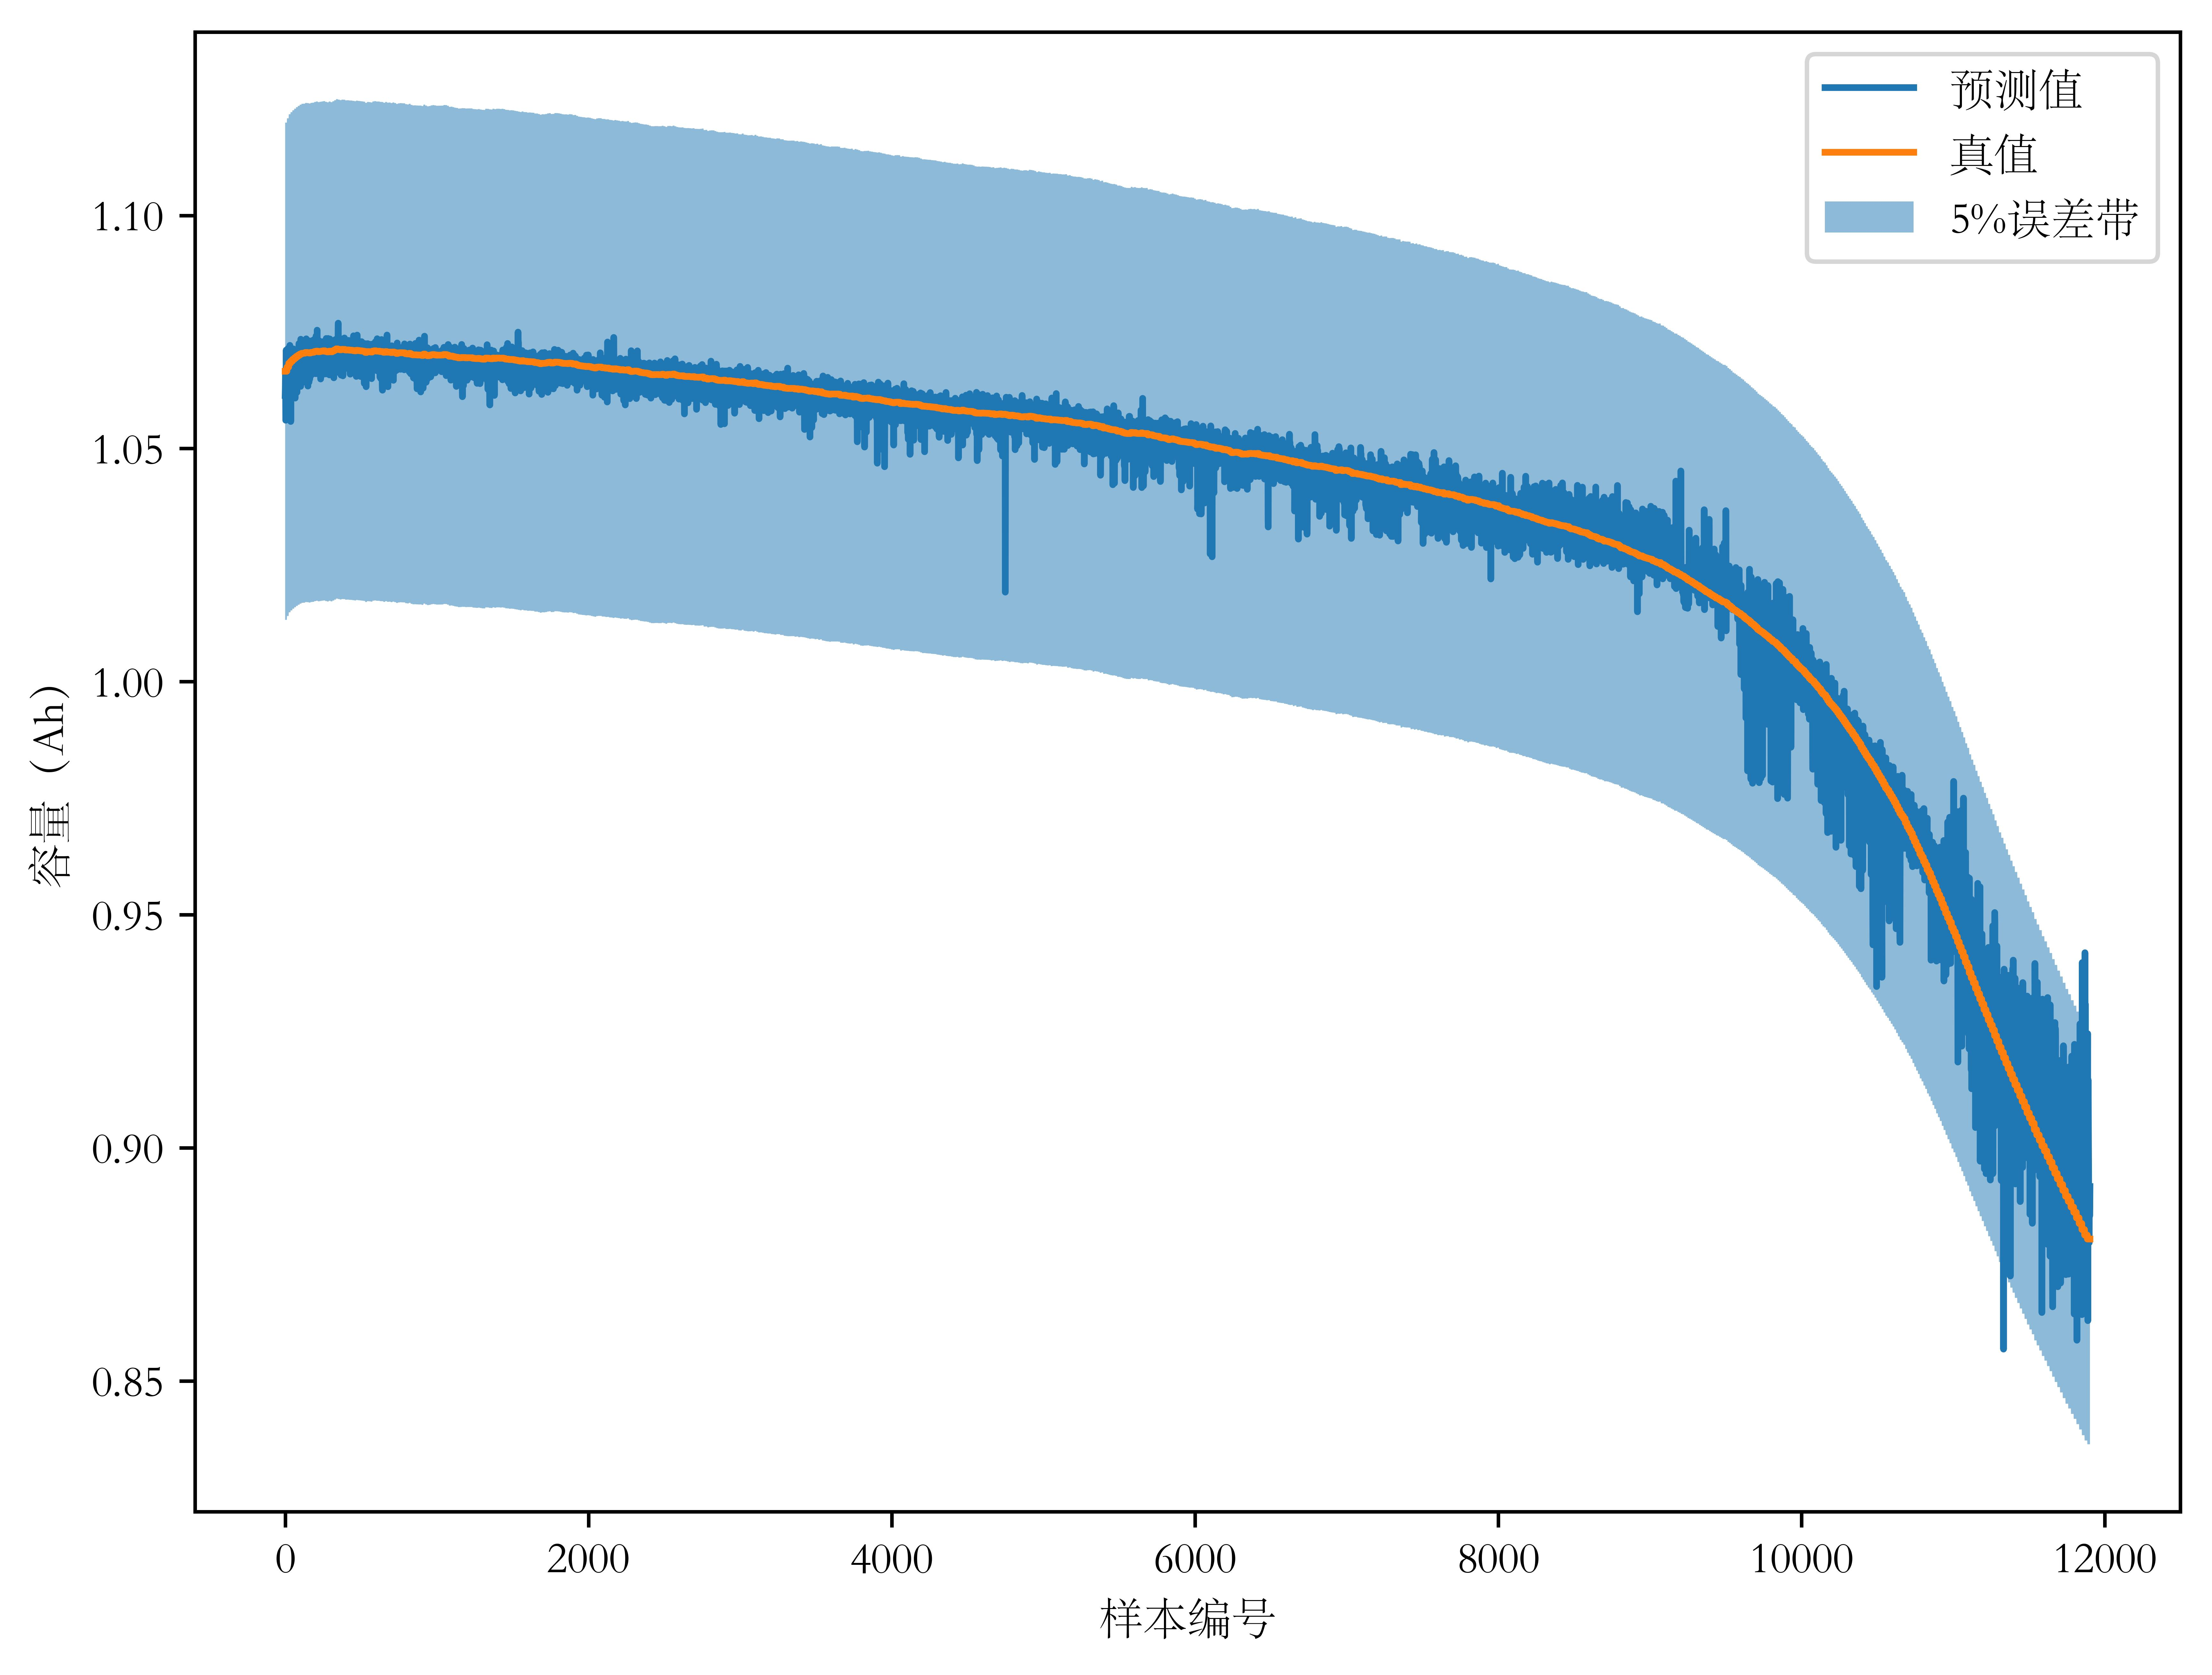
\includegraphics[width=0.2\textwidth]{figures/soh_vitq/tri_group1_cell1_cnn_viq.jpg}}
			{\label{fig:subfig3}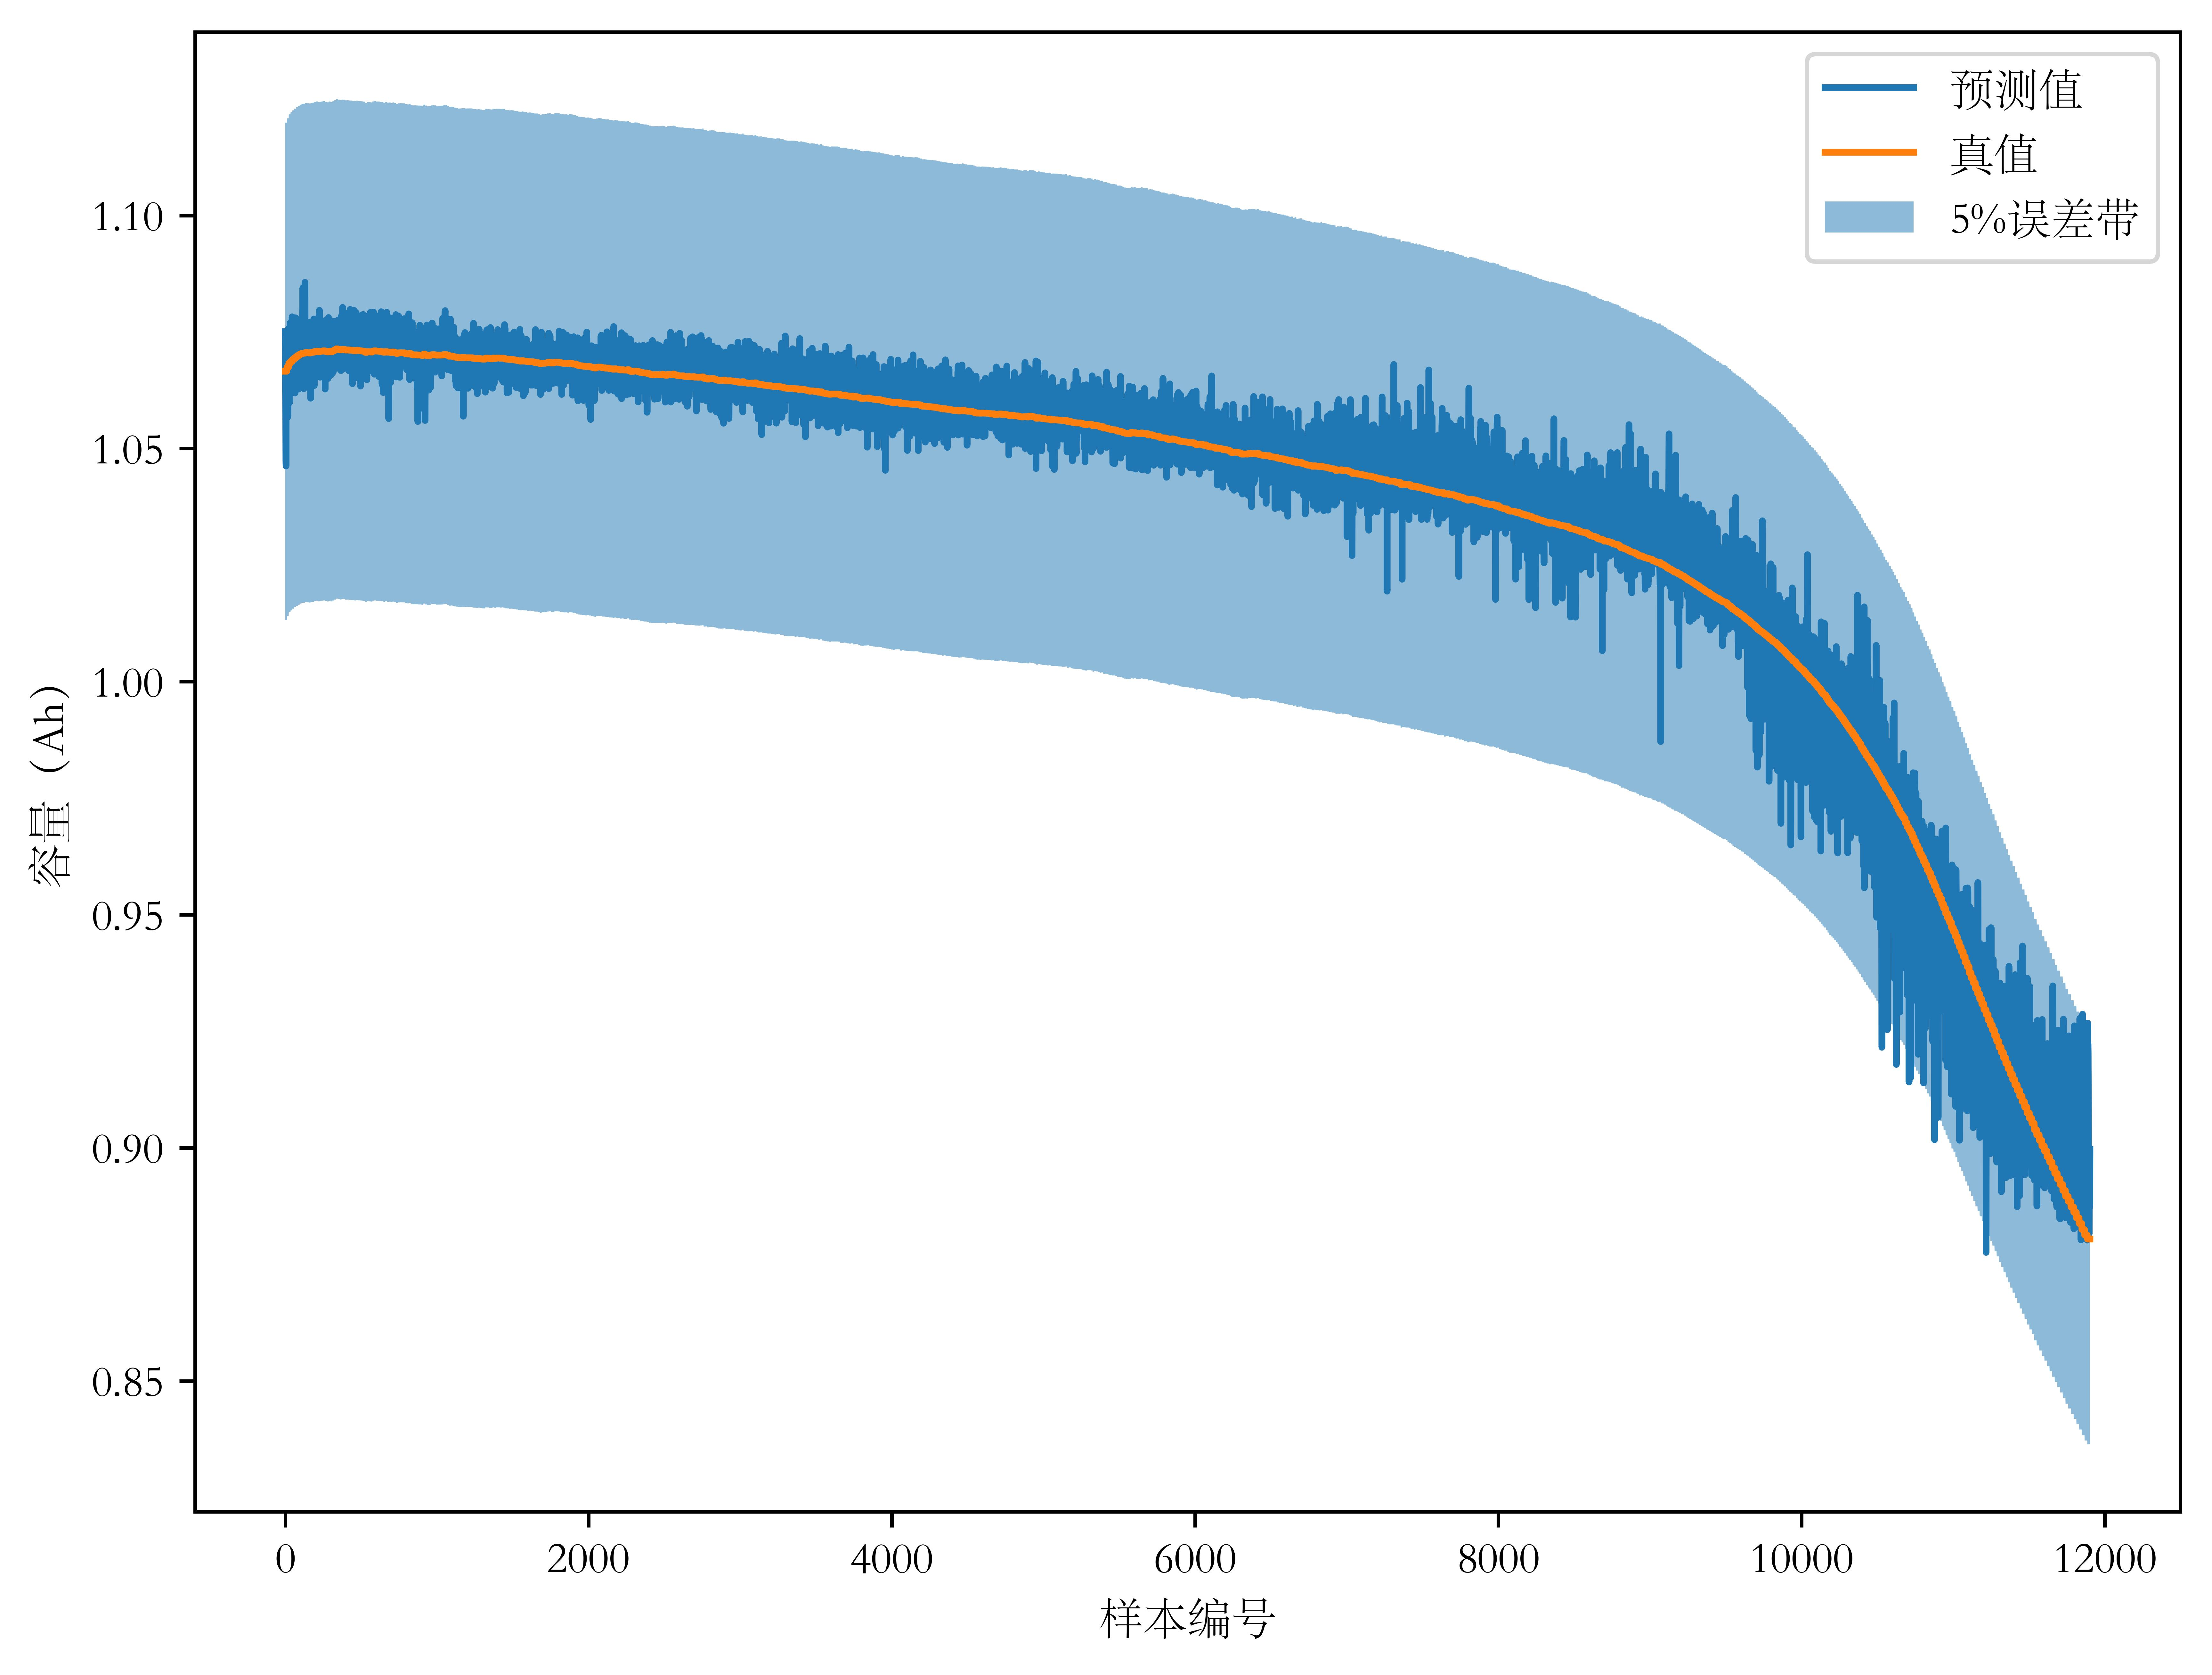
\includegraphics[width=0.2\textwidth]{figures/soh_vitq/tri_group1_cell1_cnn_vit_trans.jpg}}
			{\label{fig:subfig4}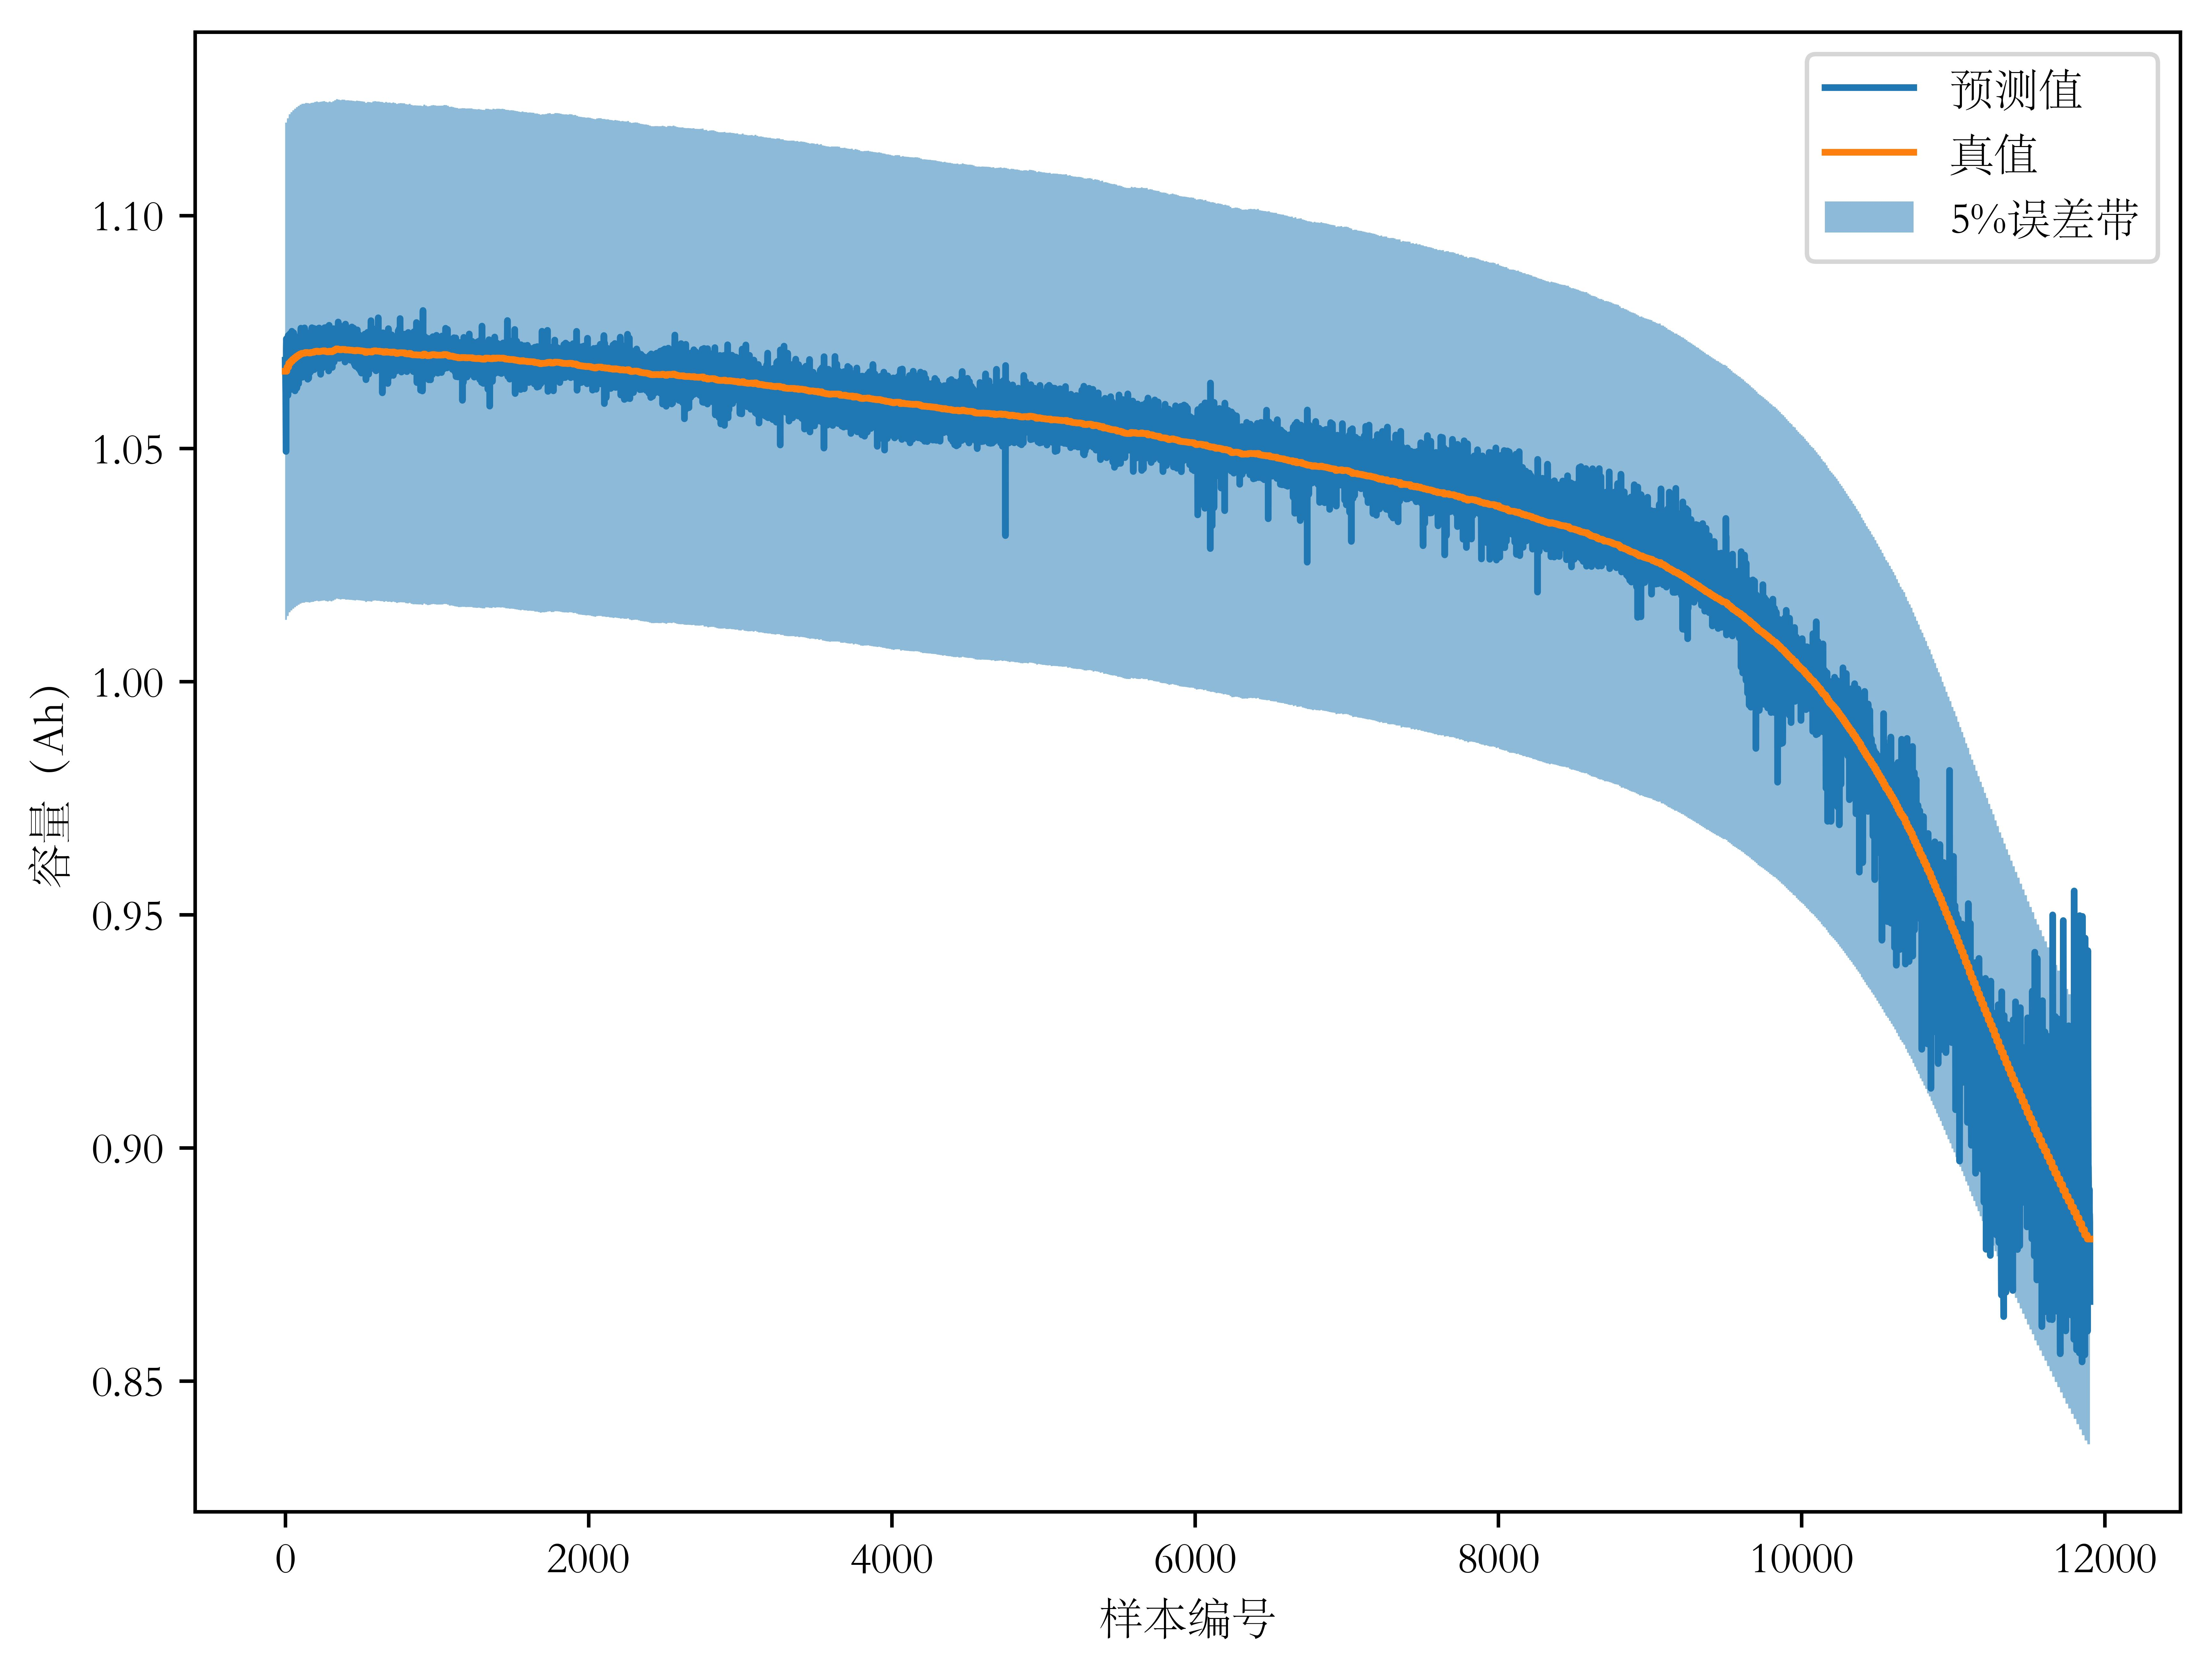
\includegraphics[width=0.2\textwidth]{figures/soh_vitq/tri_group1_cell1_cnn_viq_trans.jpg}}
	\end{figure}
	\begin{figure}[htbp]
		\centering
			{\label{fig:subfig1}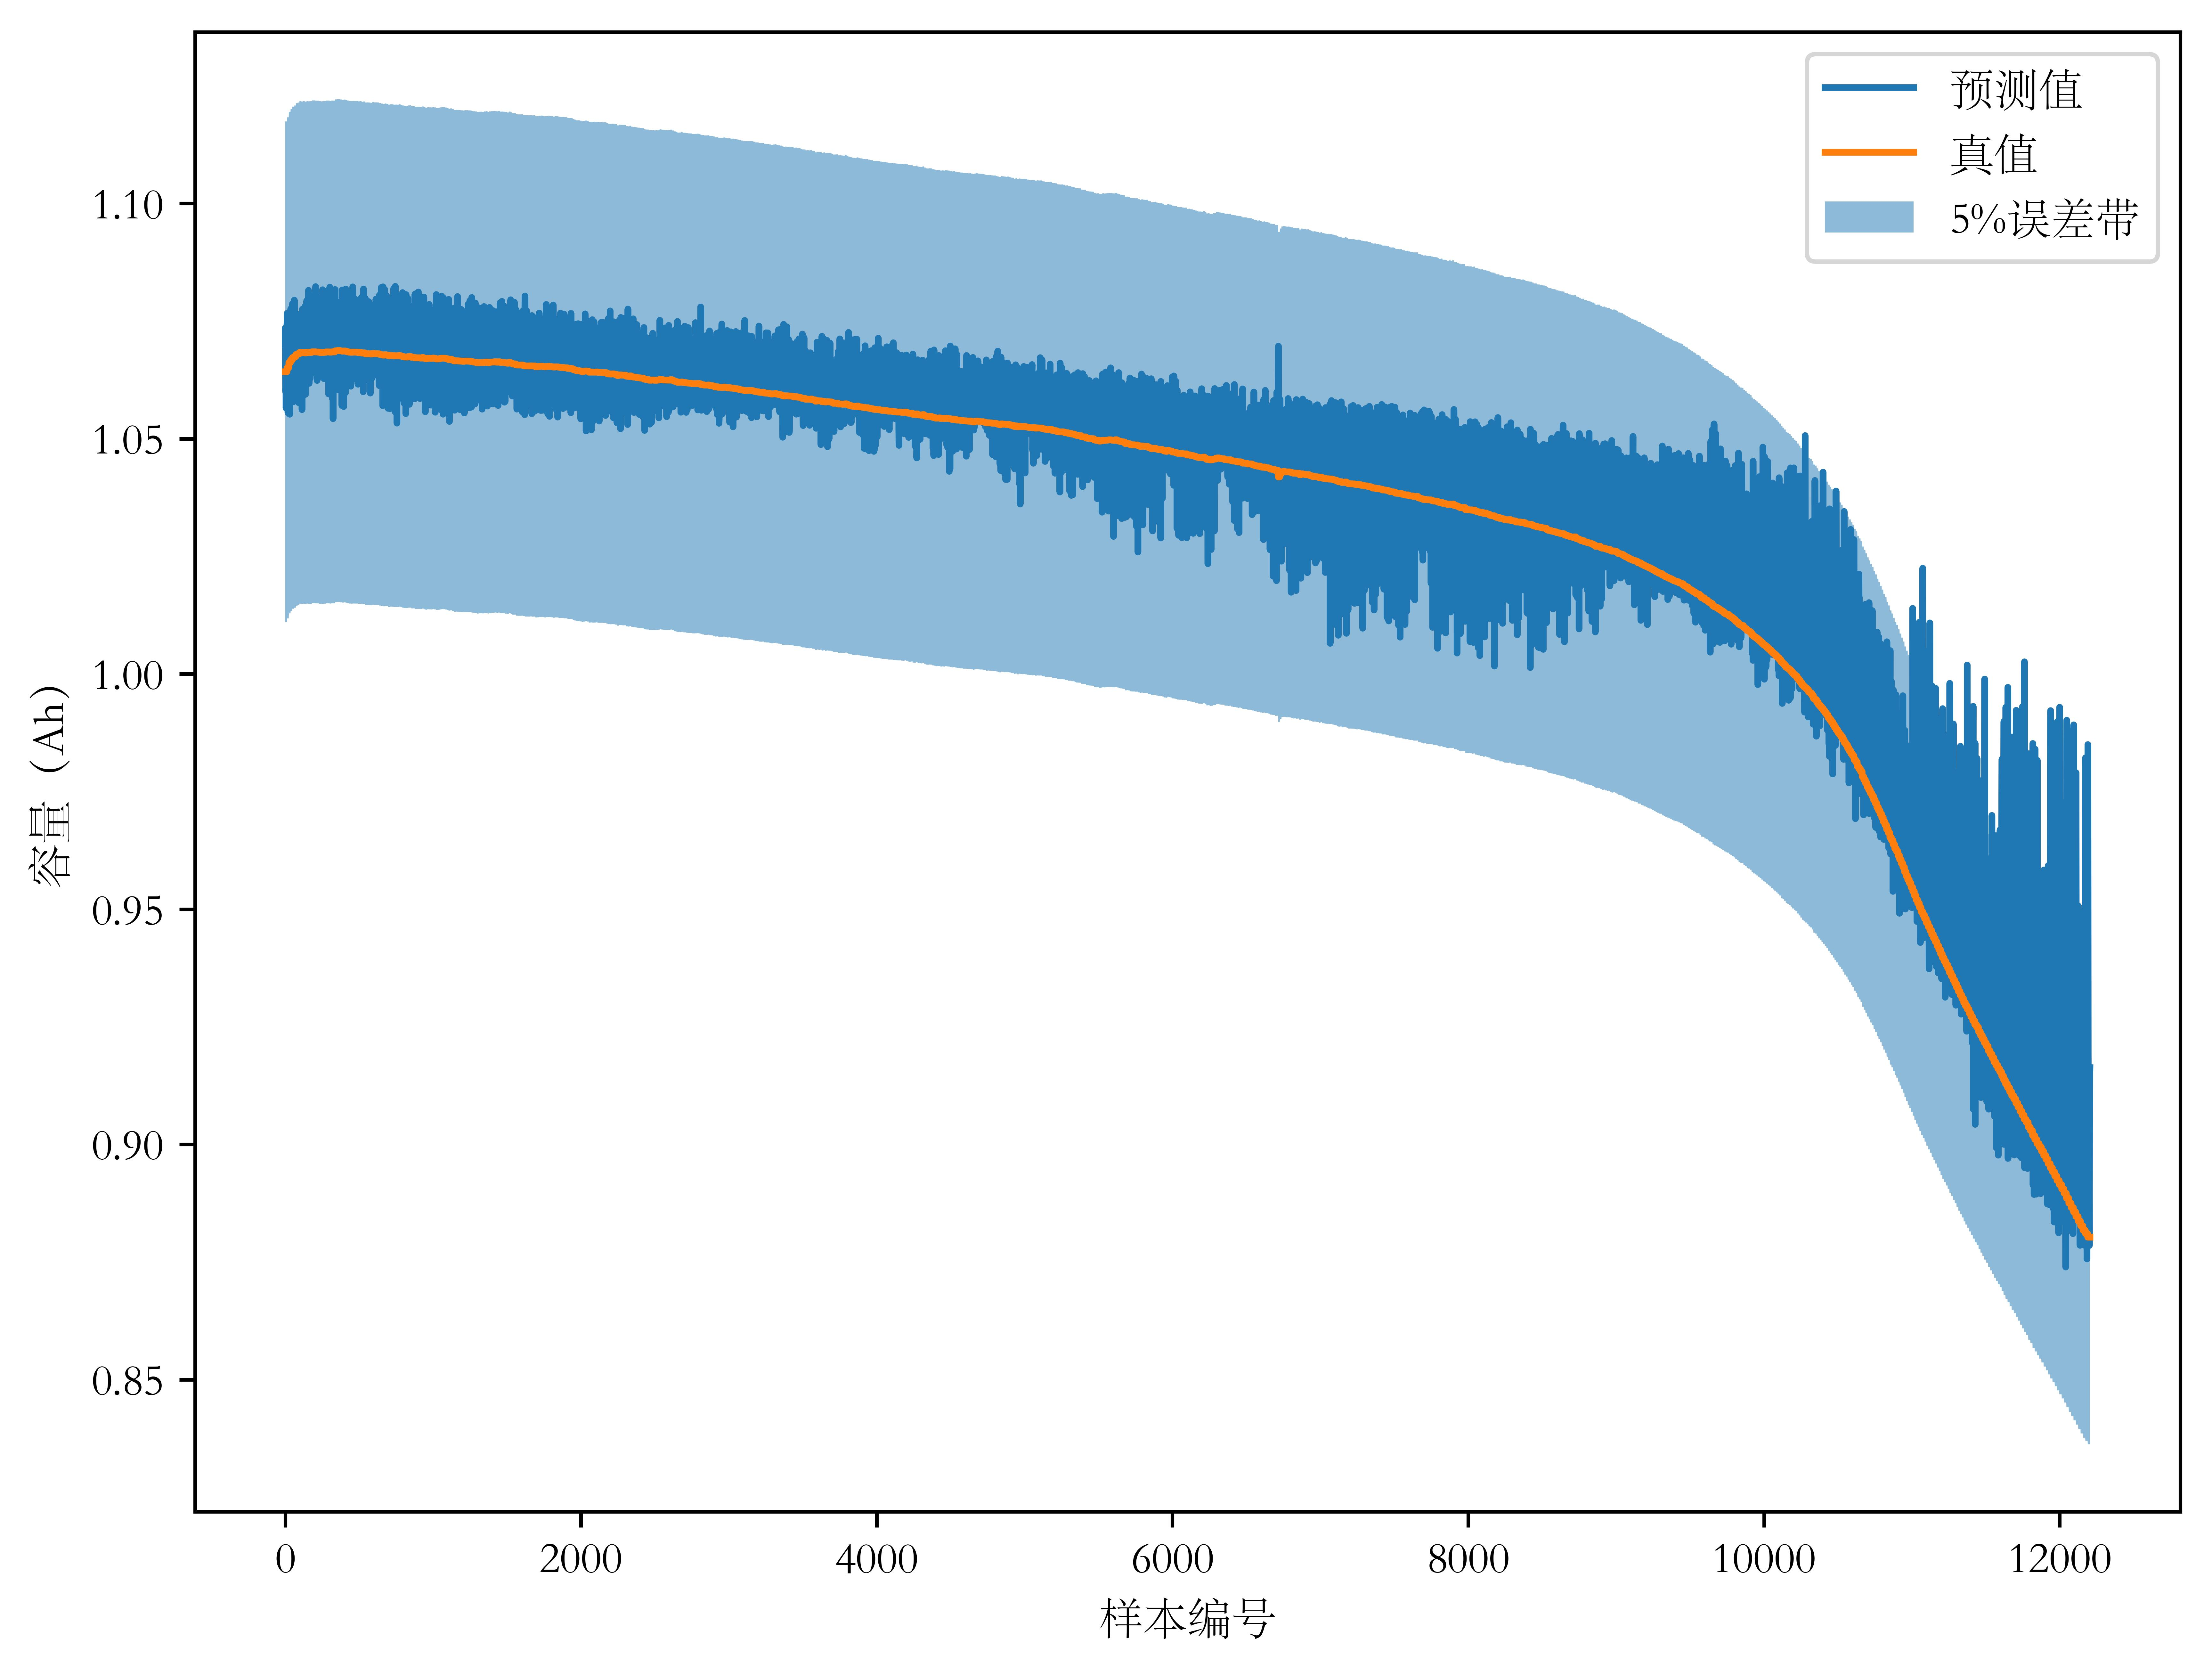
\includegraphics[width=0.2\textwidth]{figures/soh_vitq/tri_group1_cell2_cnn_vit.jpg}}
			{\label{fig:subfig2}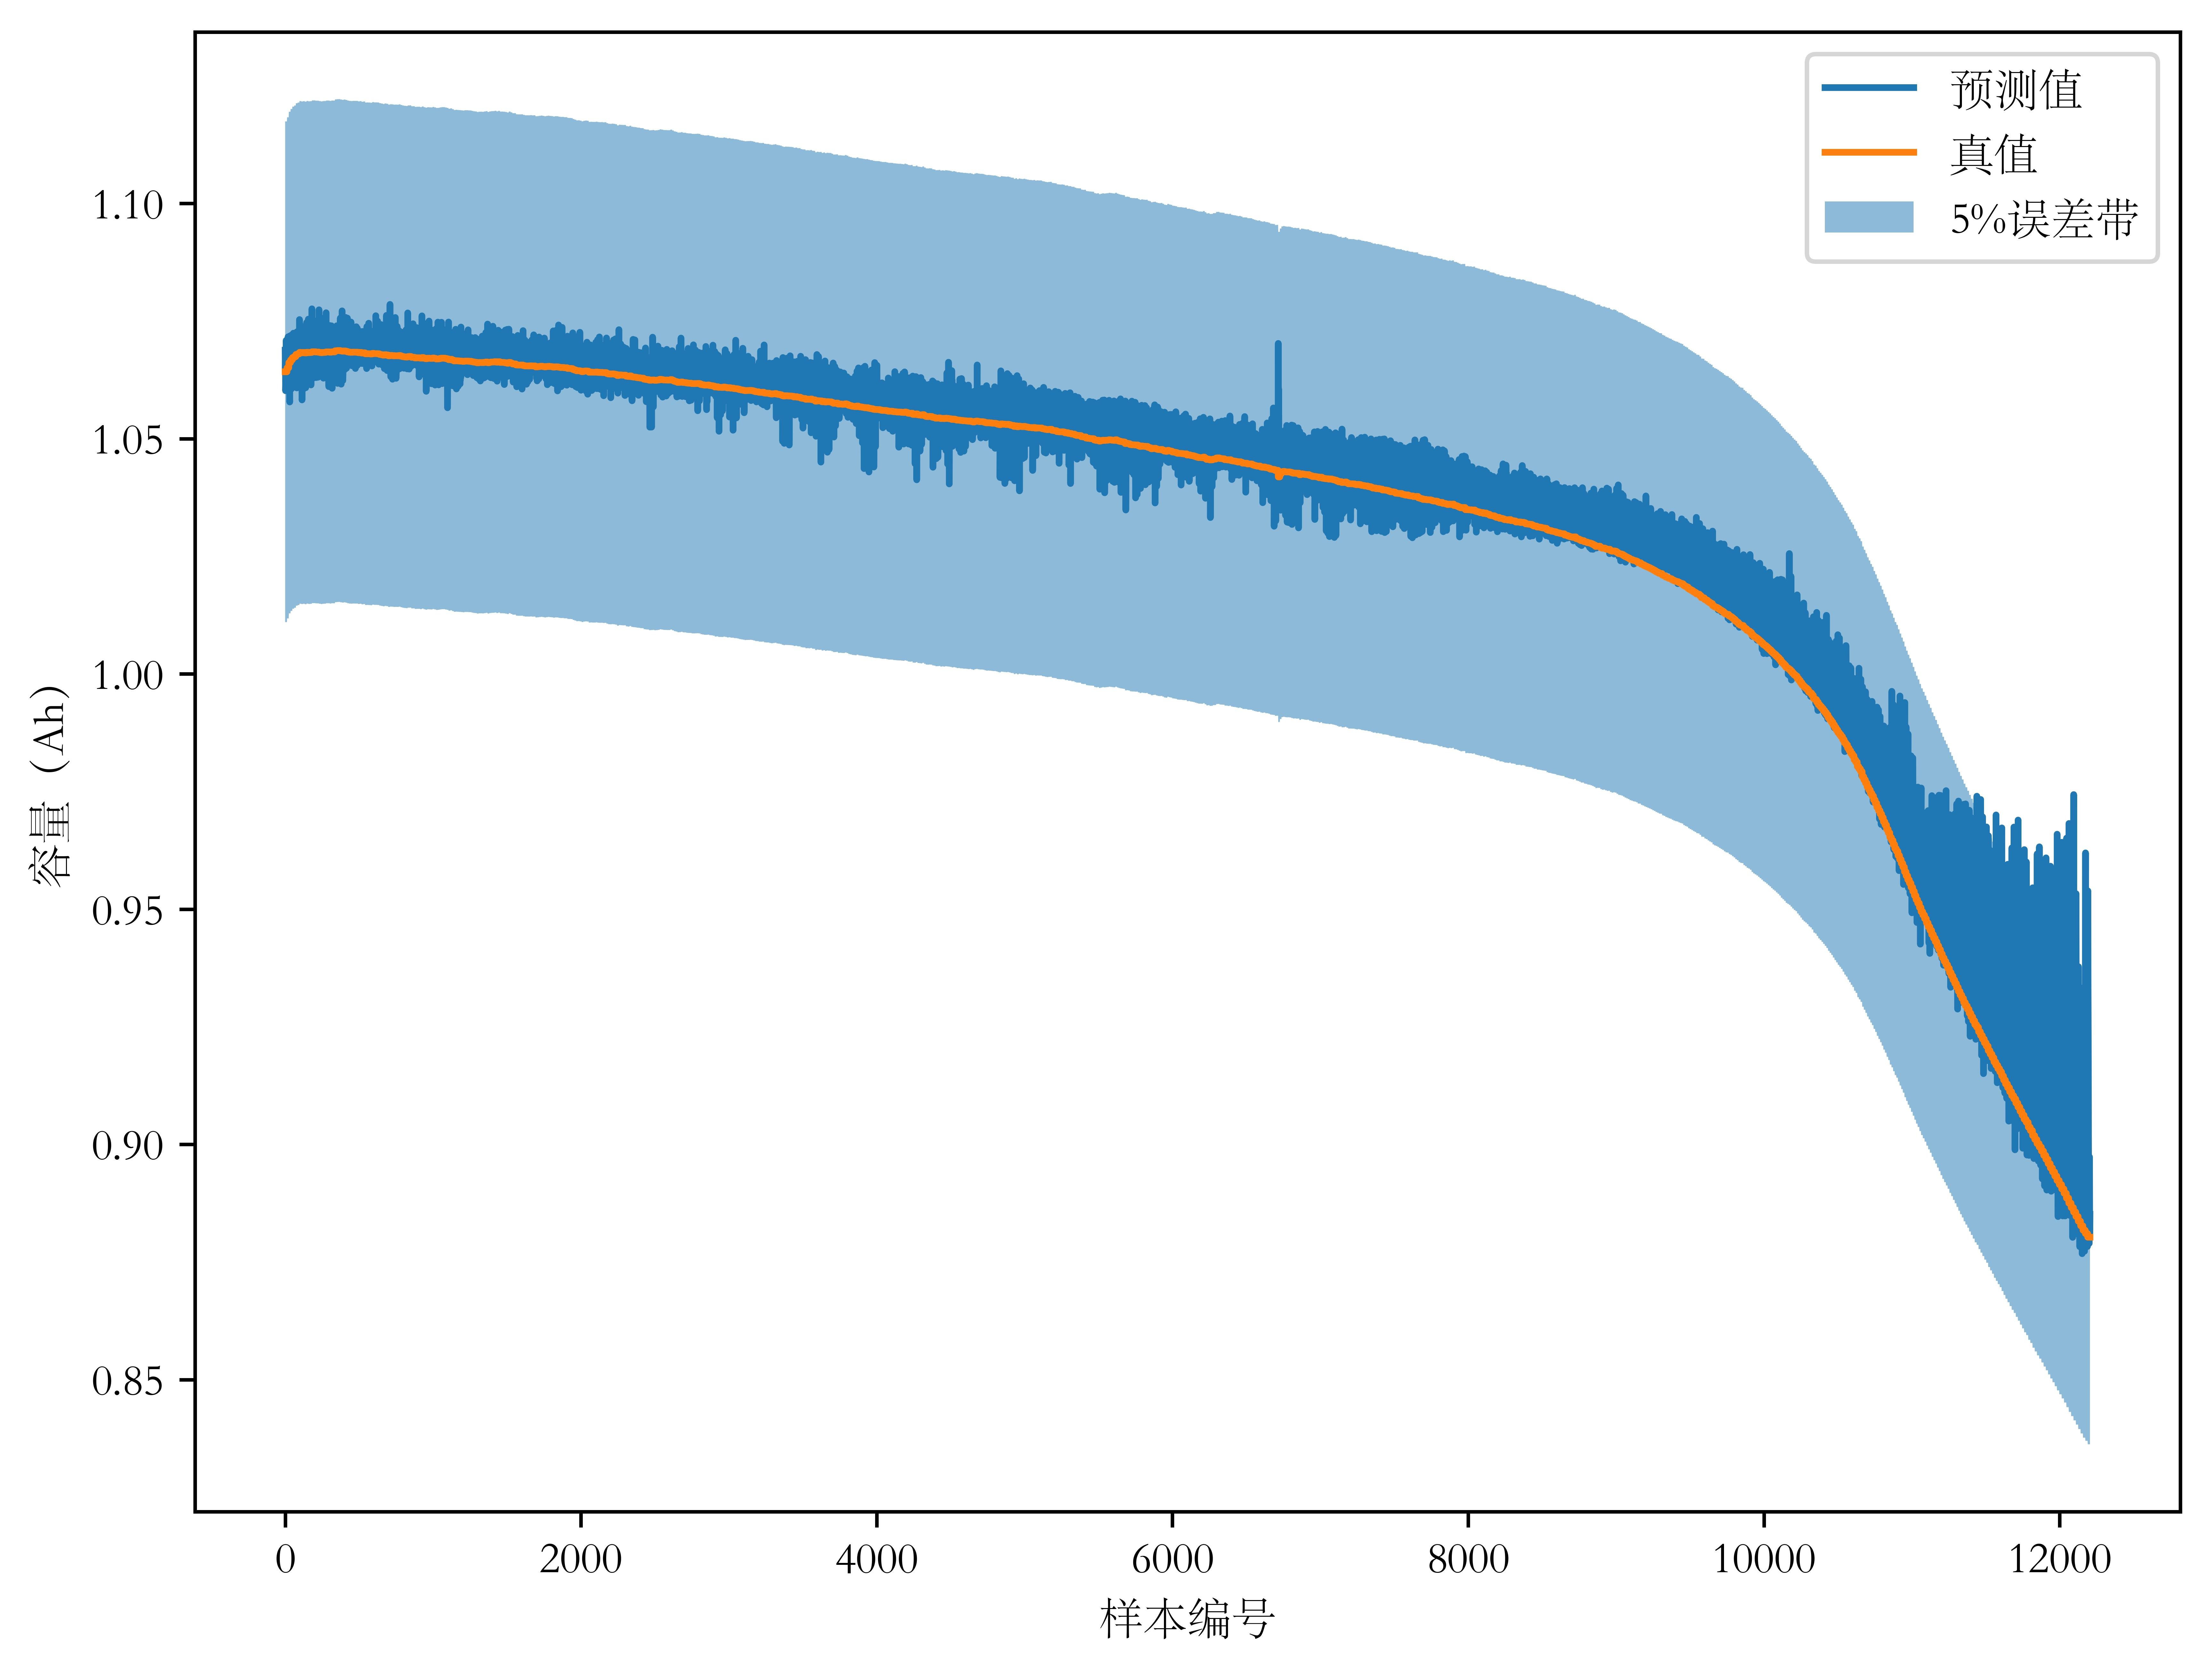
\includegraphics[width=0.2\textwidth]{figures/soh_vitq/tri_group1_cell2_cnn_viq.jpg}}
			{\label{fig:subfig3}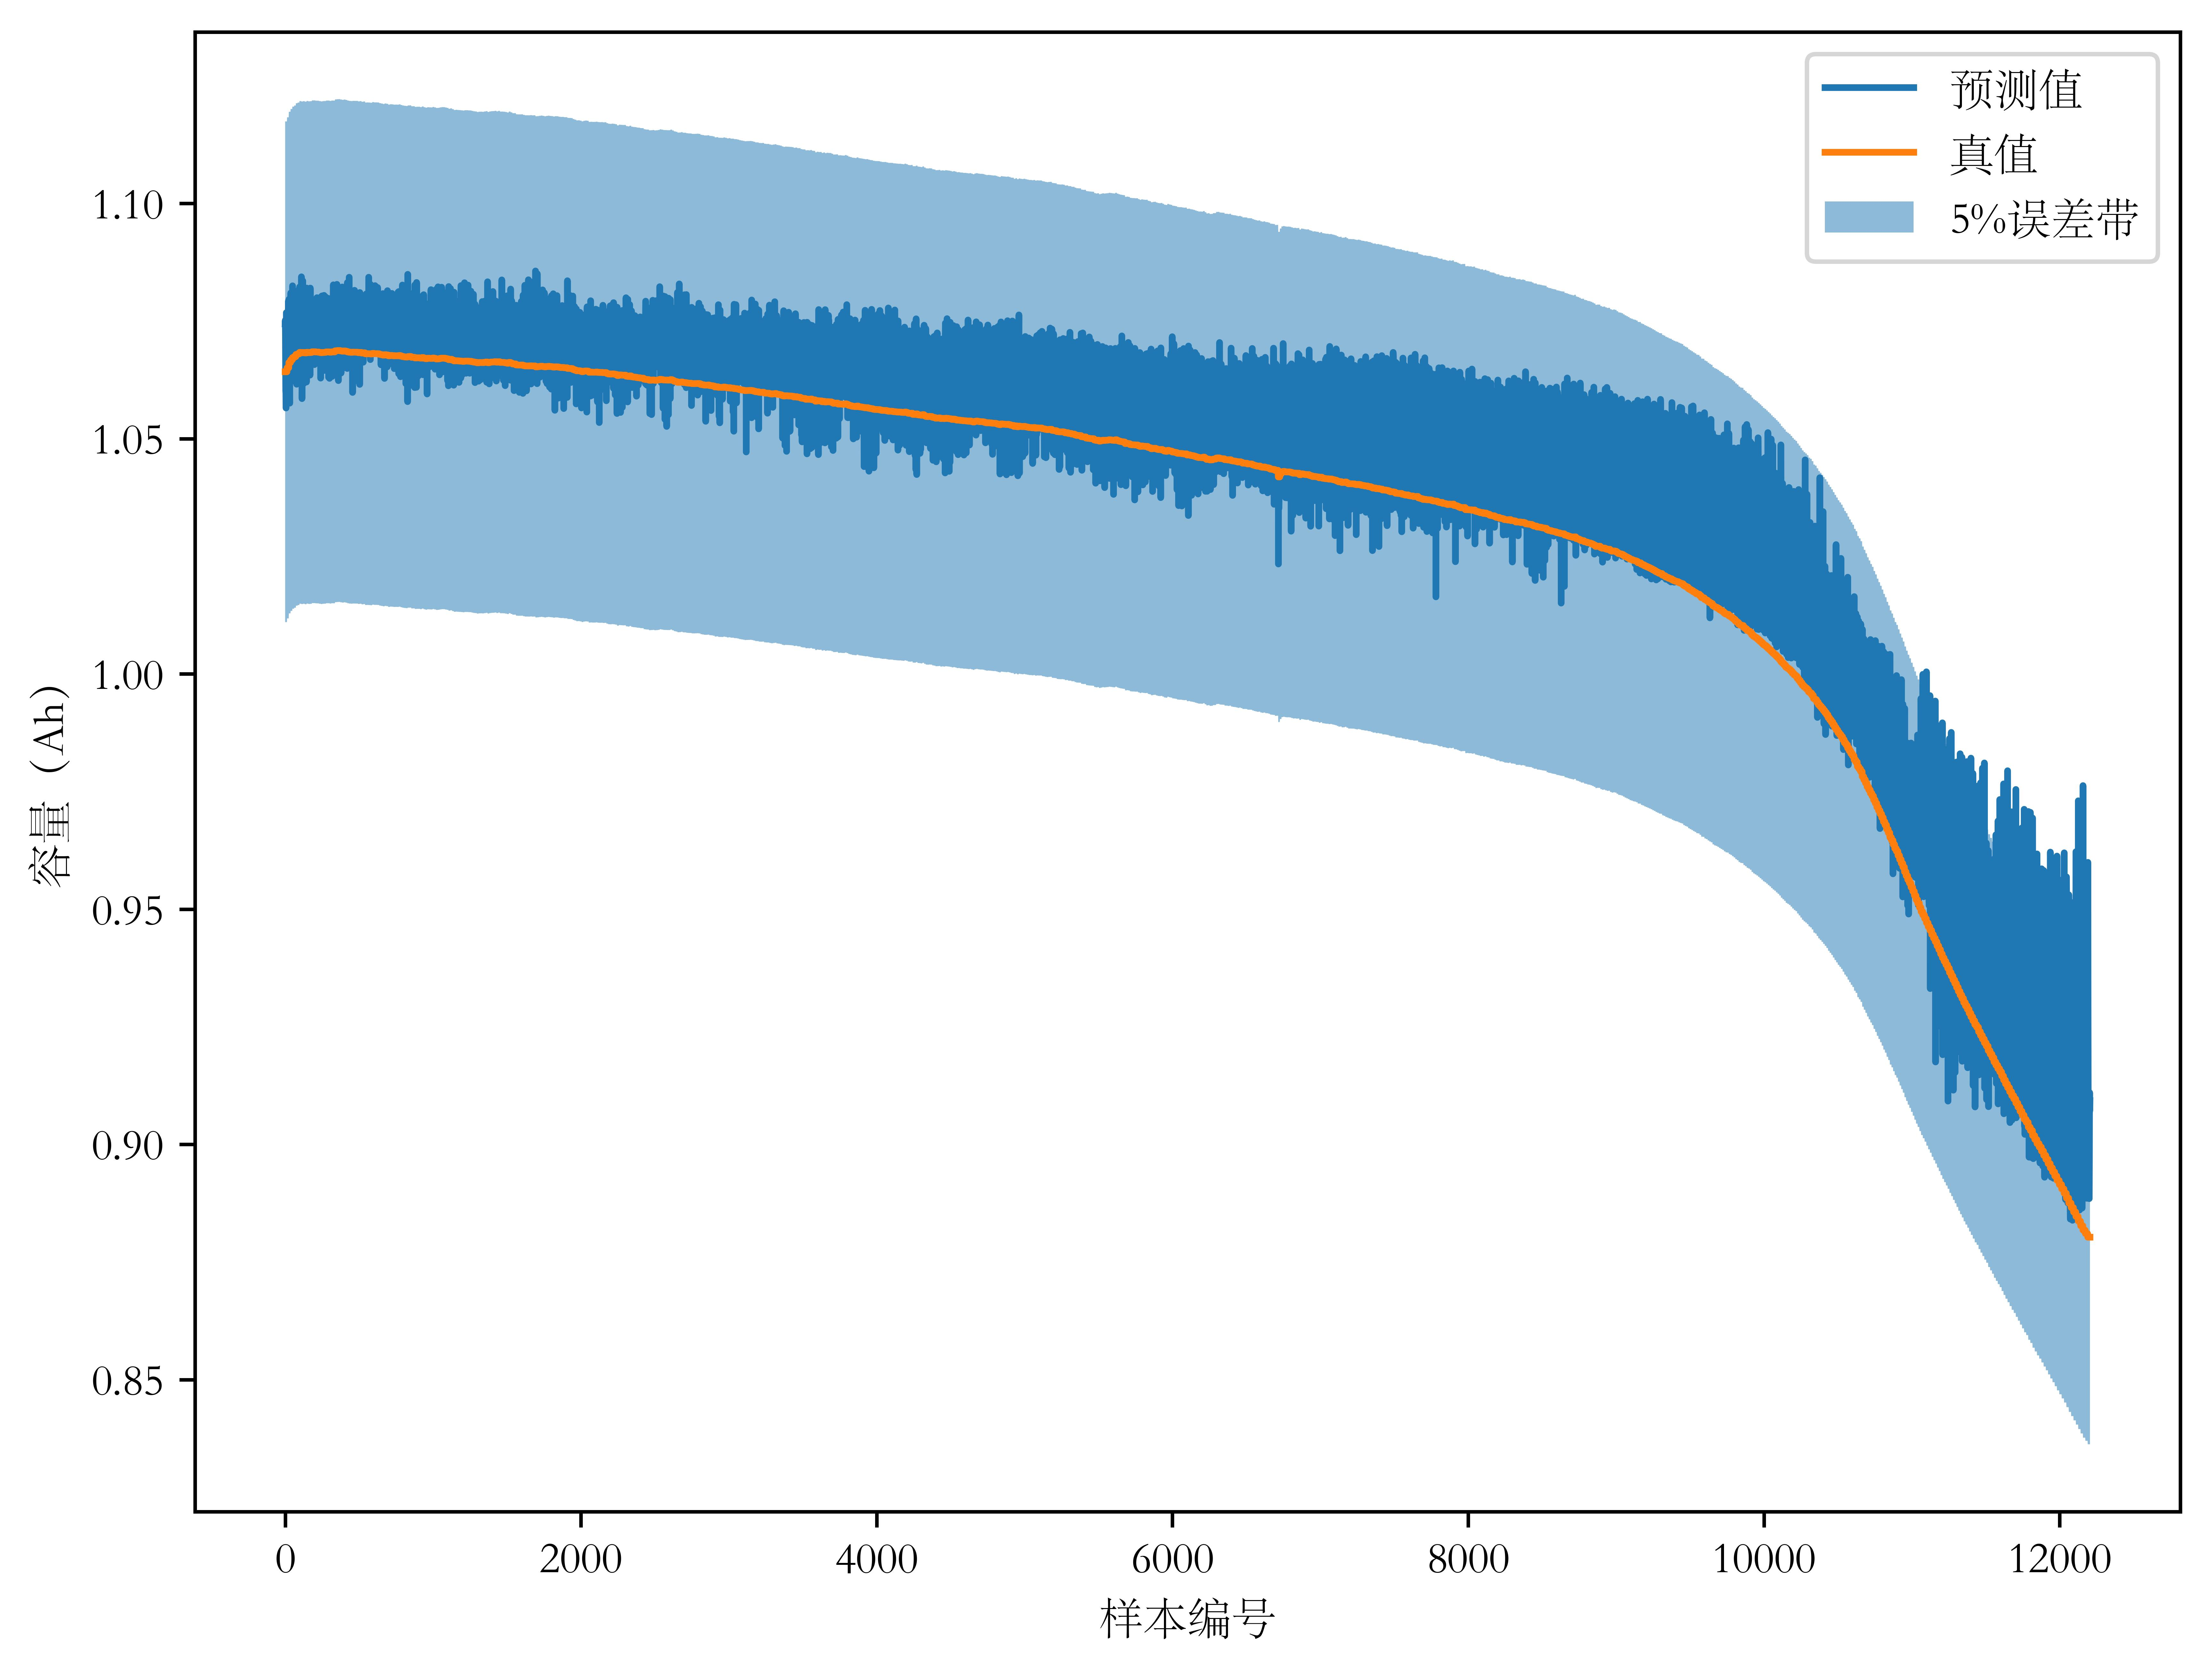
\includegraphics[width=0.2\textwidth]{figures/soh_vitq/tri_group1_cell2_cnn_vit_trans.jpg}}
			{\label{fig:subfig4}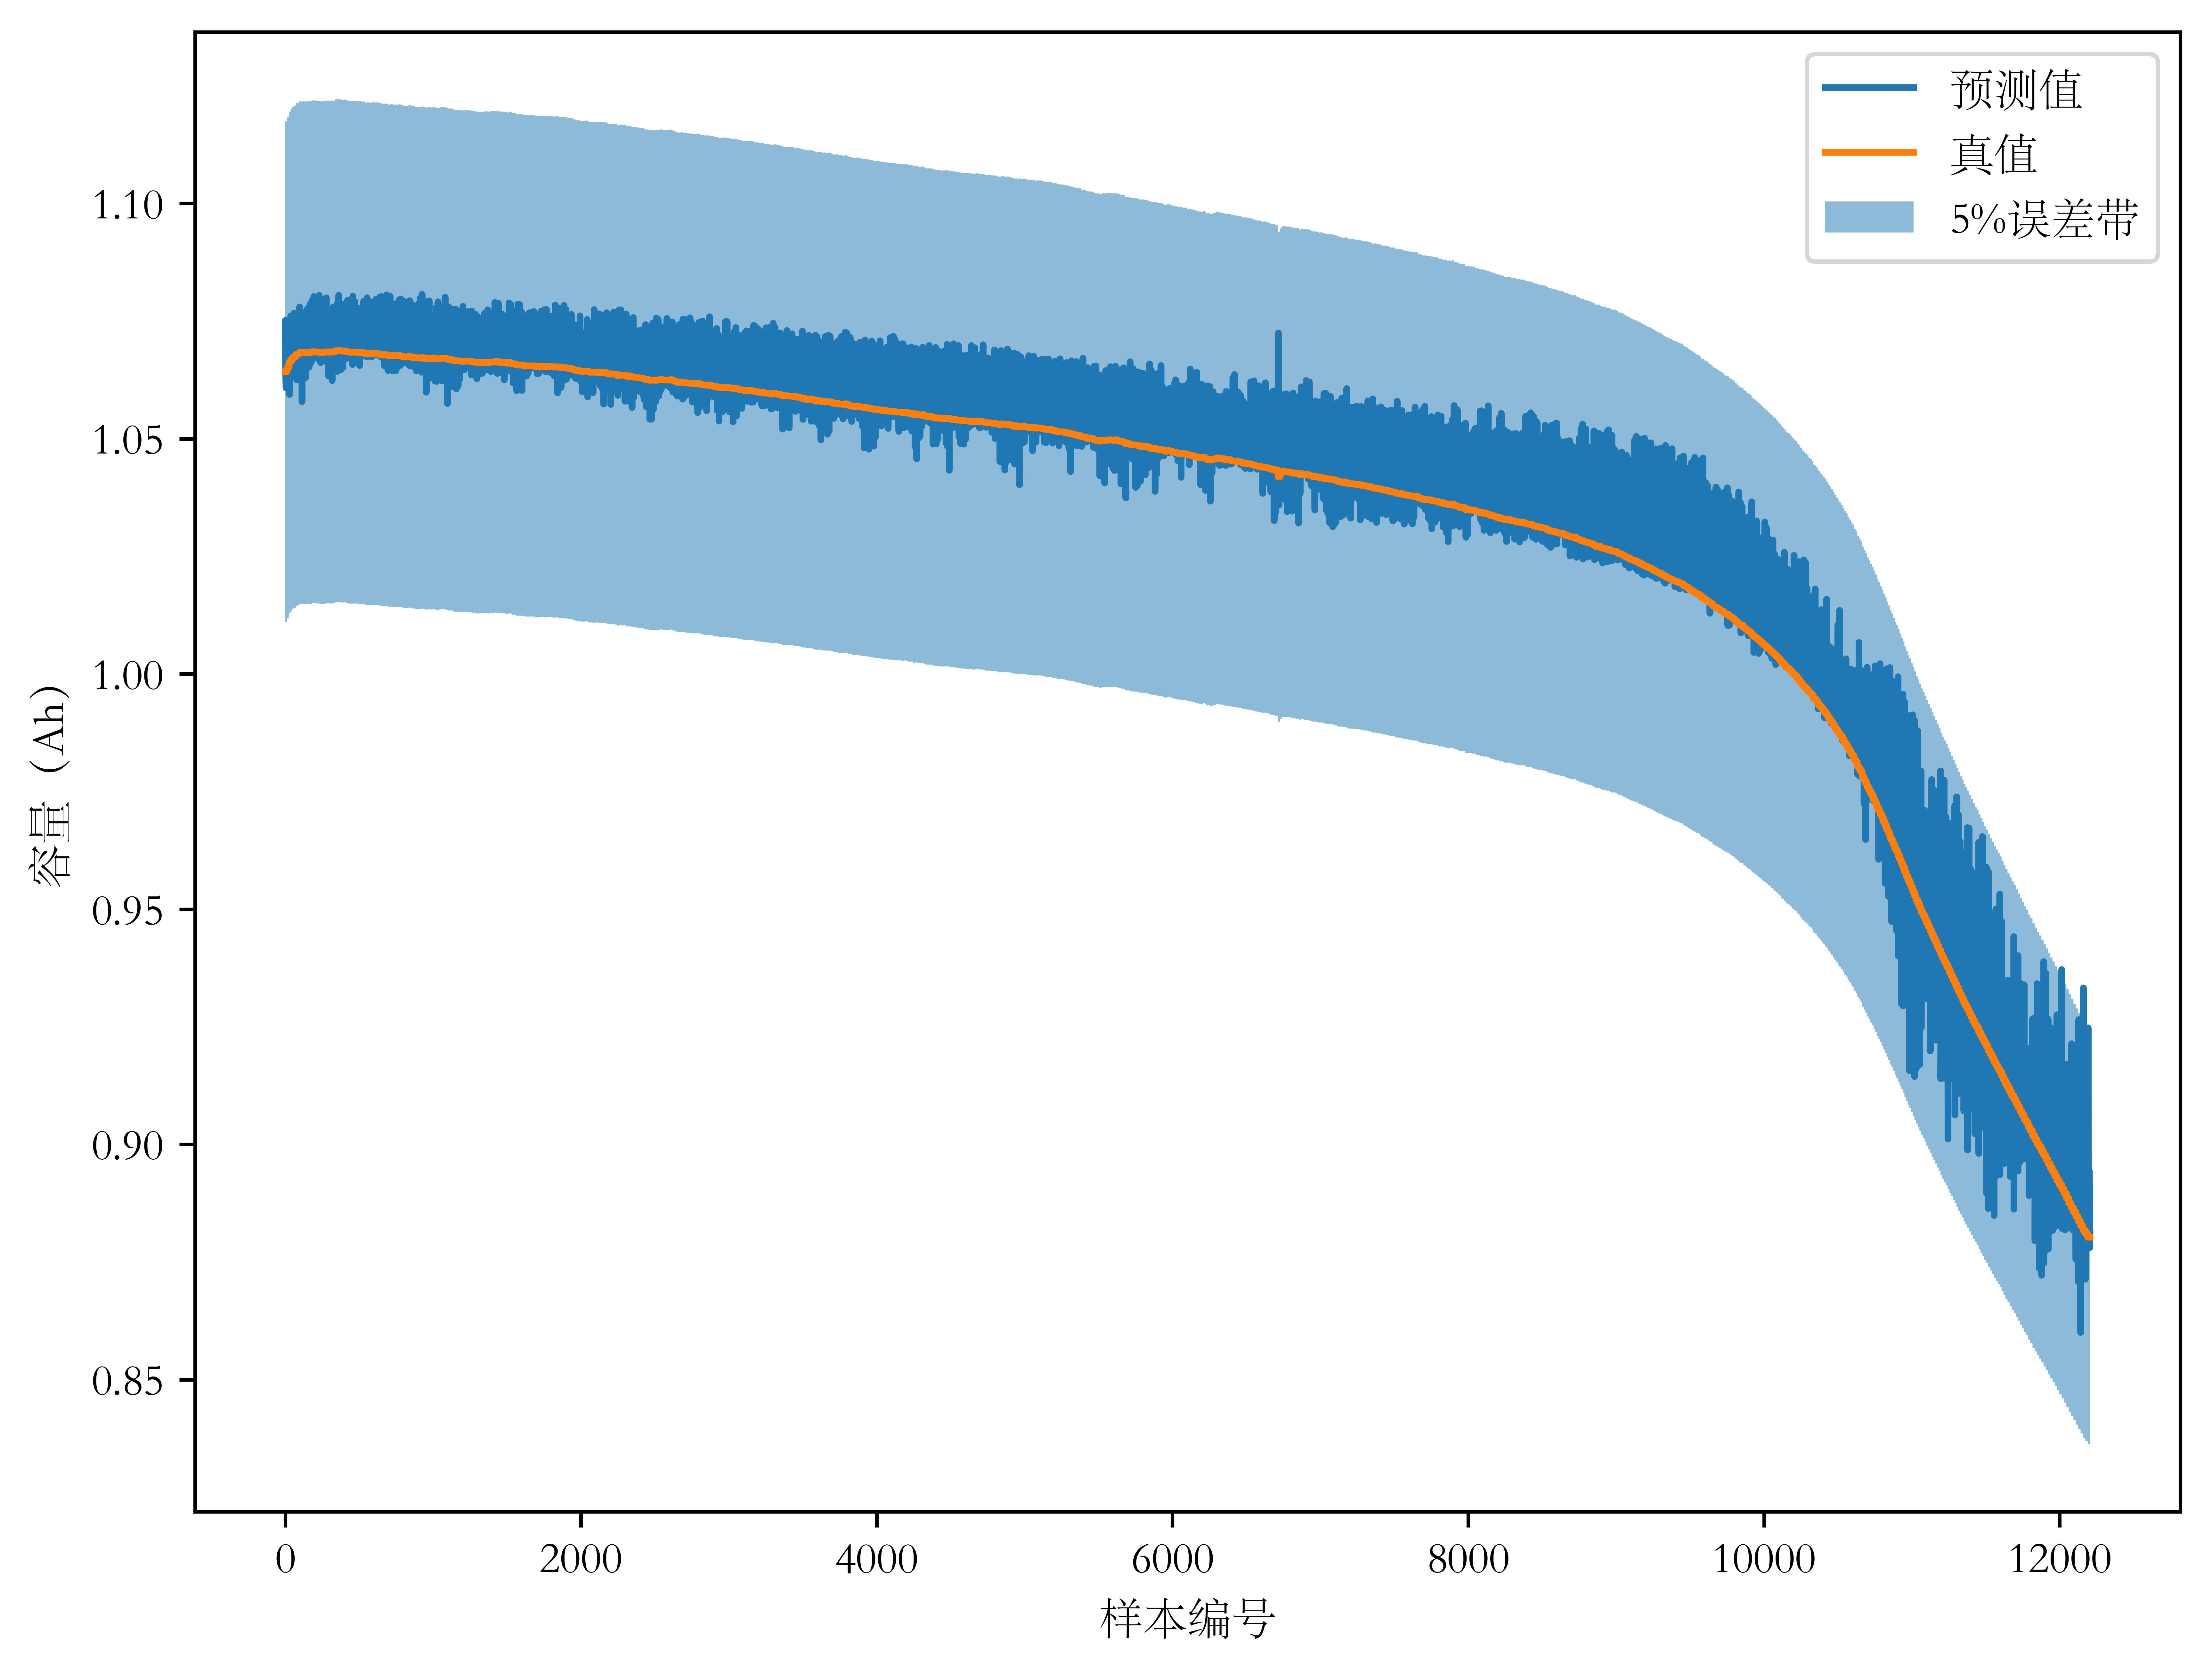
\includegraphics[width=0.2\textwidth]{figures/soh_vitq/tri_group1_cell2_cnn_viq_trans.jpg}}
	\end{figure}
	\begin{figure}[htbp]
		\centering
			{\label{fig:subfig1}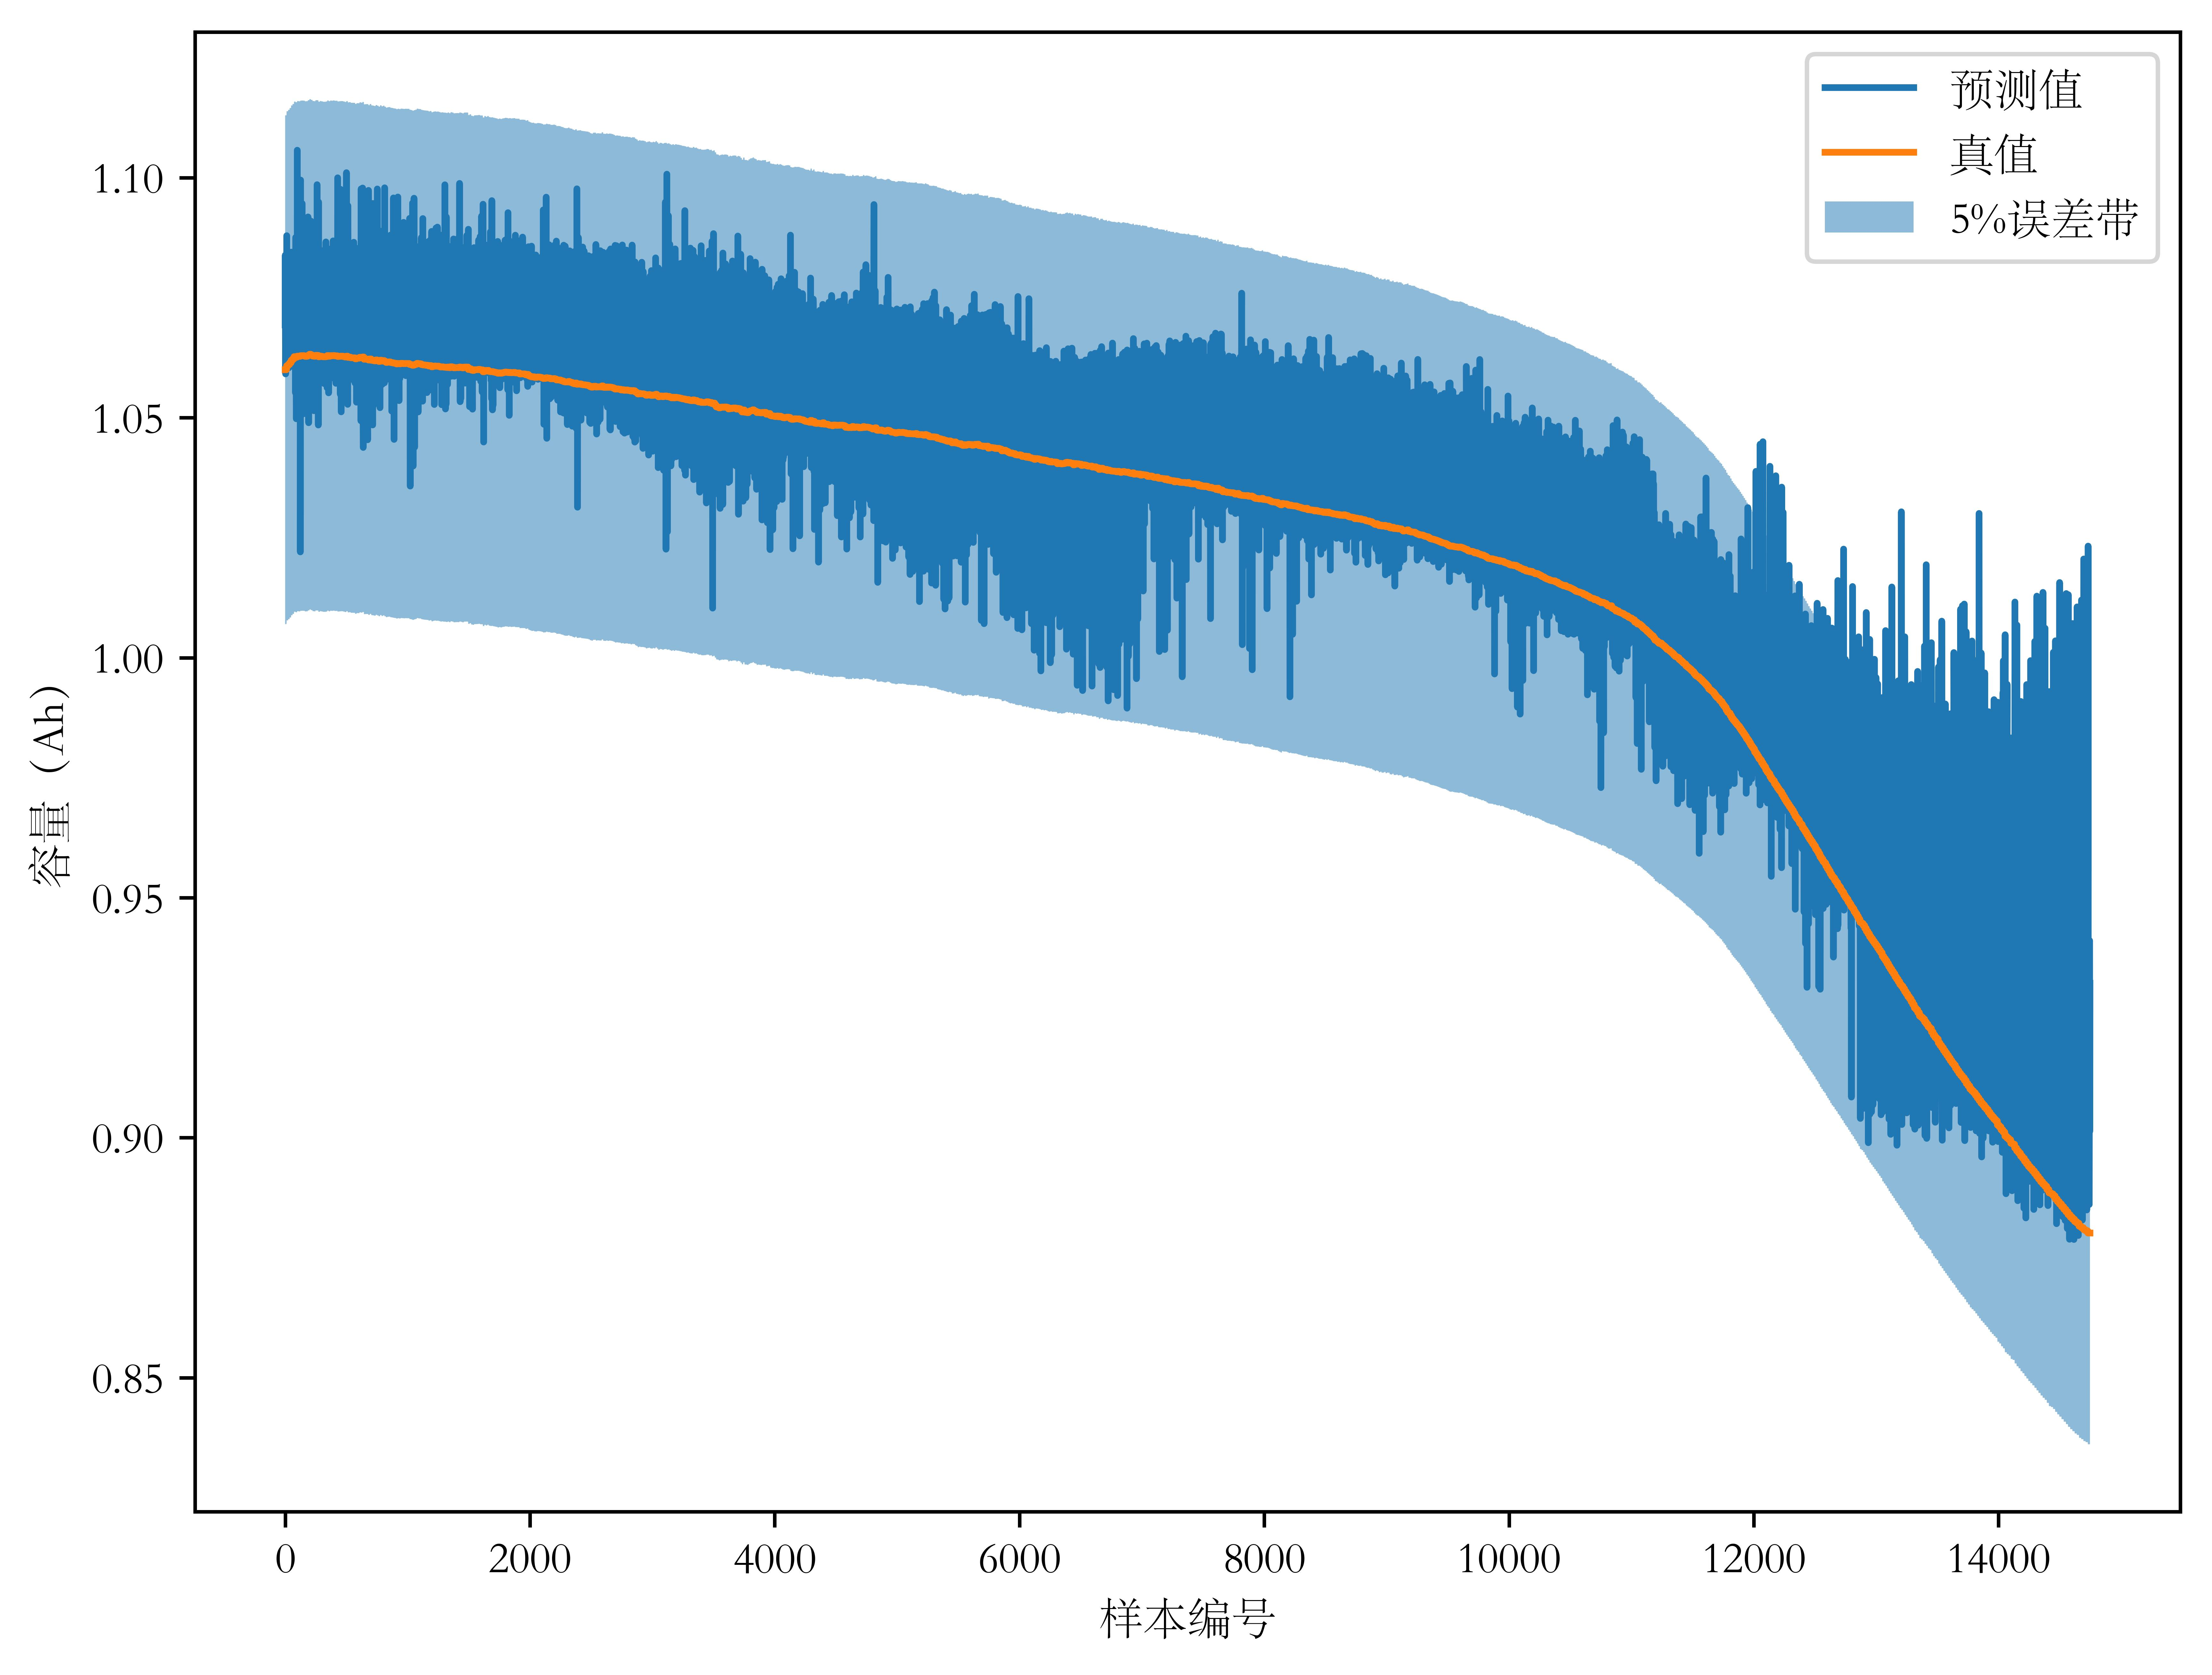
\includegraphics[width=0.2\textwidth]{figures/soh_vitq/tri_group1_cell3_cnn_vit.jpg}}
			{\label{fig:subfig2}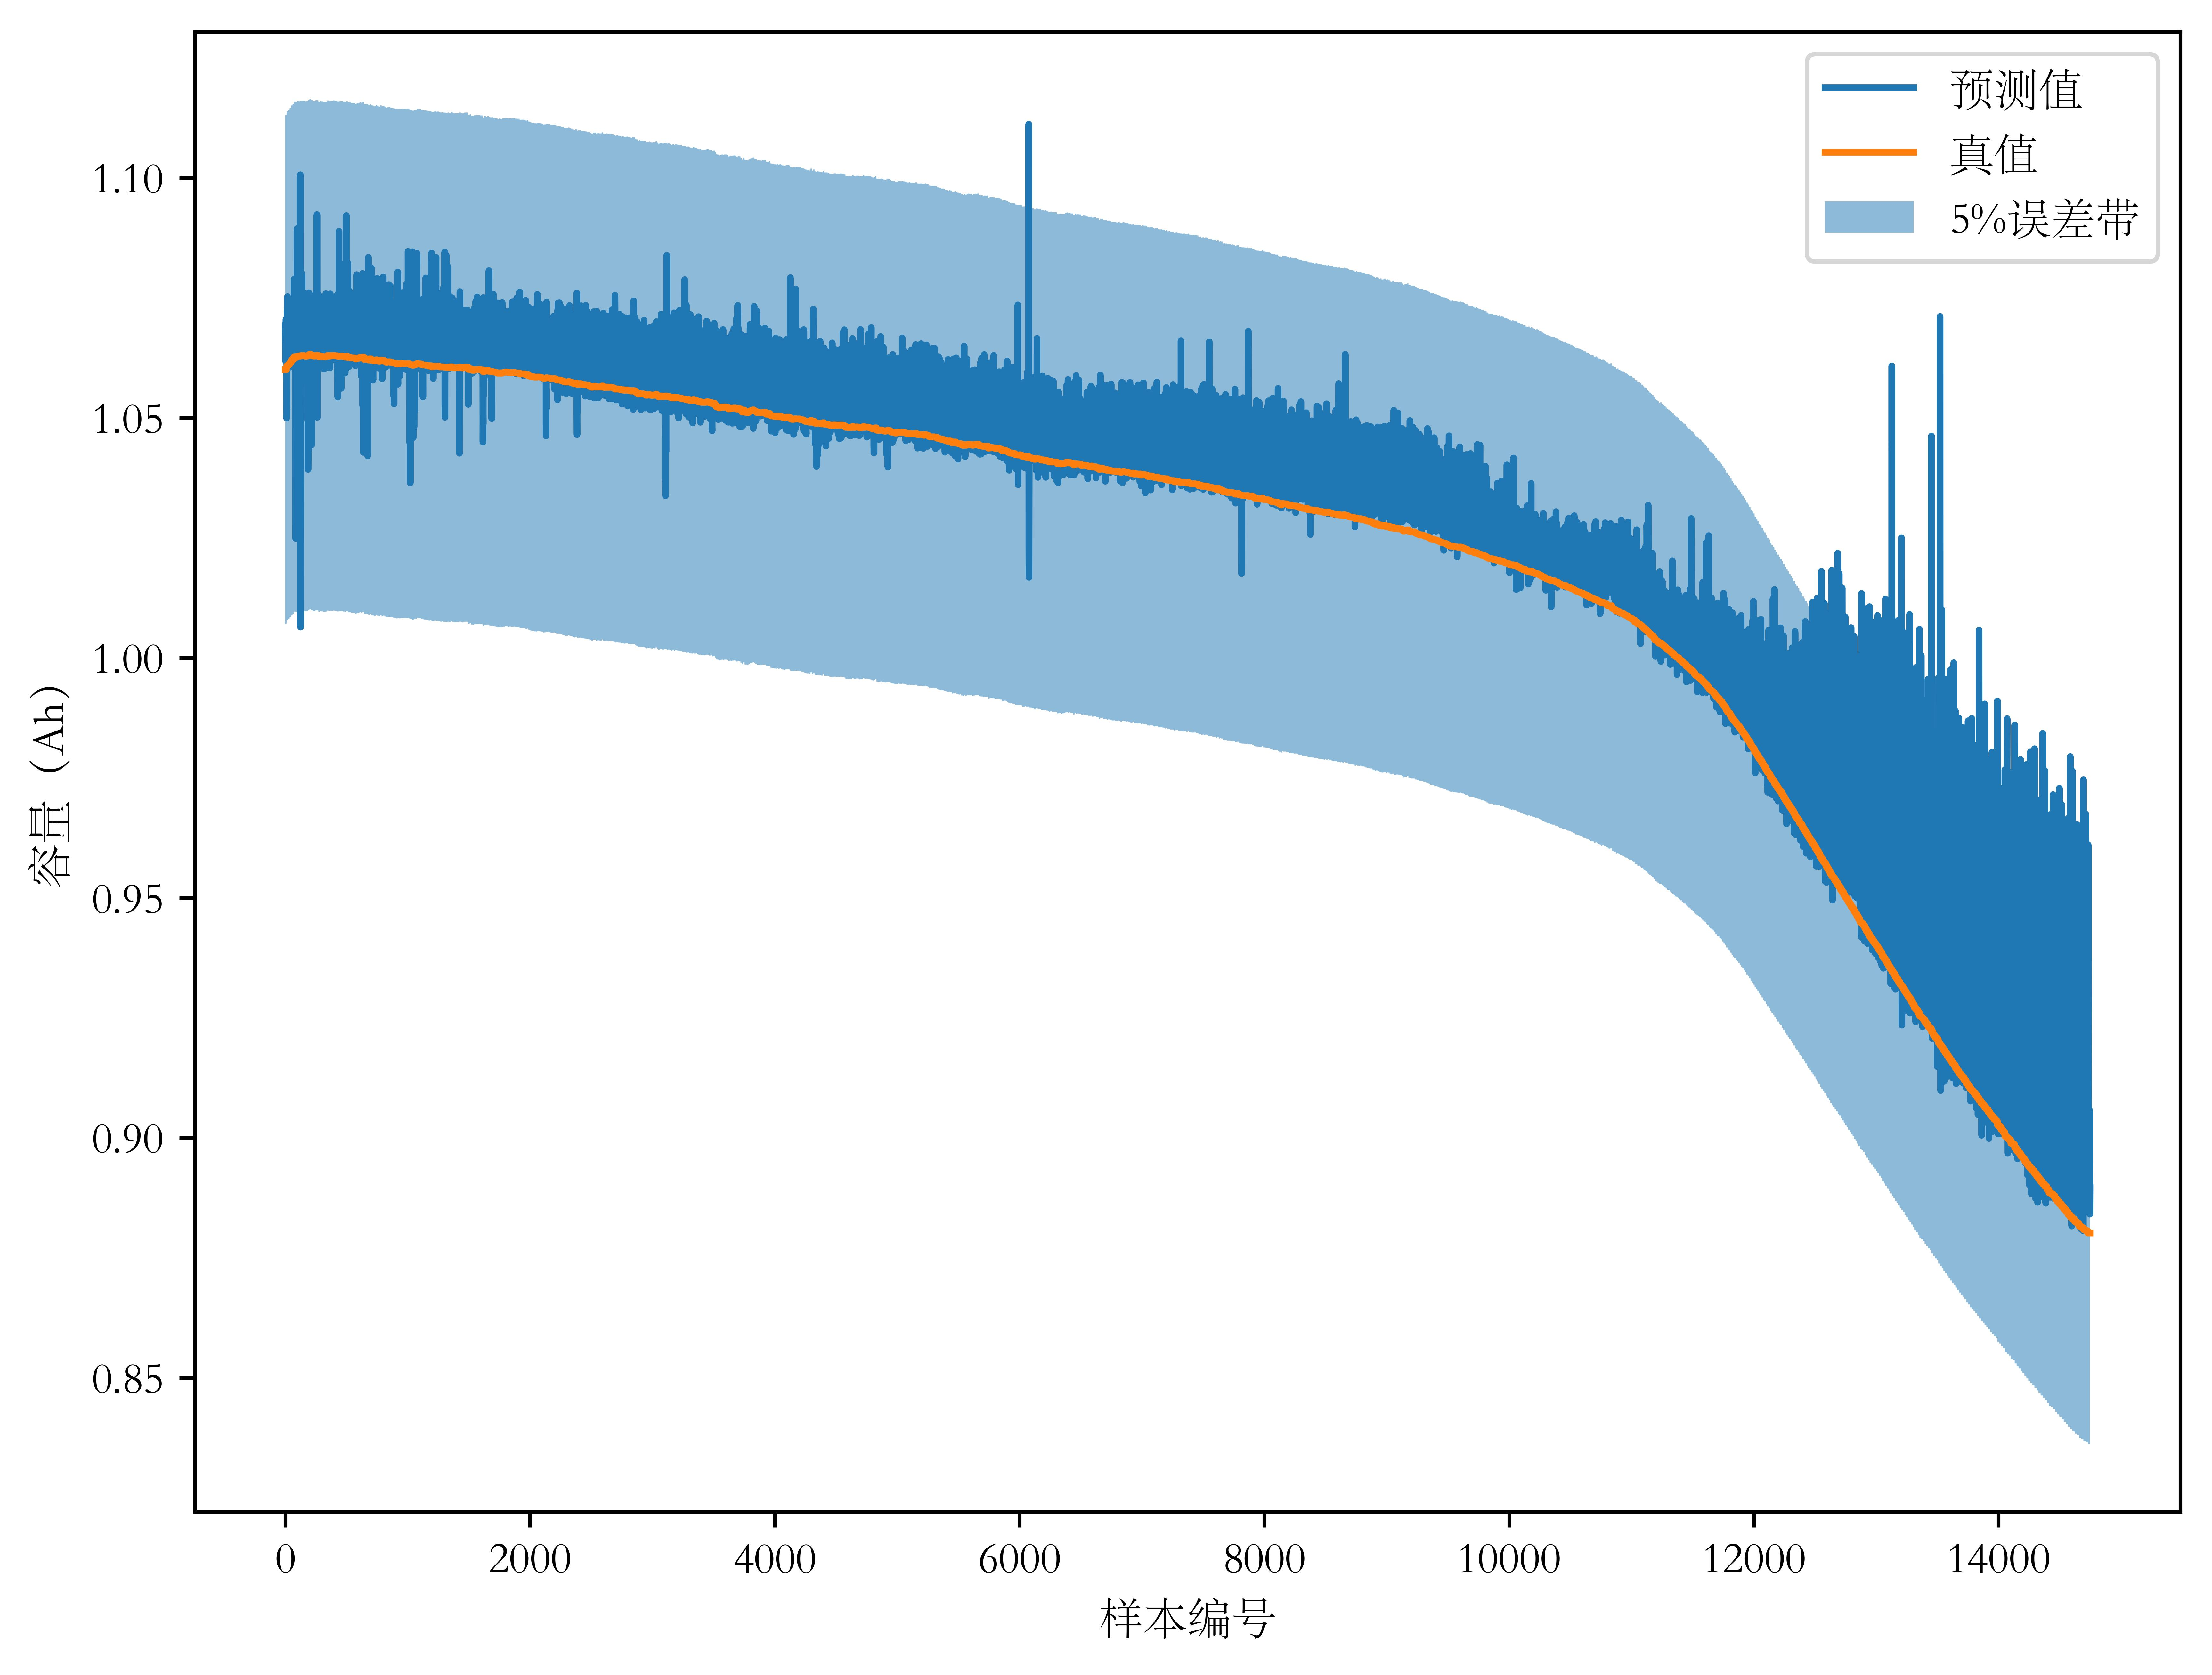
\includegraphics[width=0.2\textwidth]{figures/soh_vitq/tri_group1_cell3_cnn_viq.jpg}}
			{\label{fig:subfig3}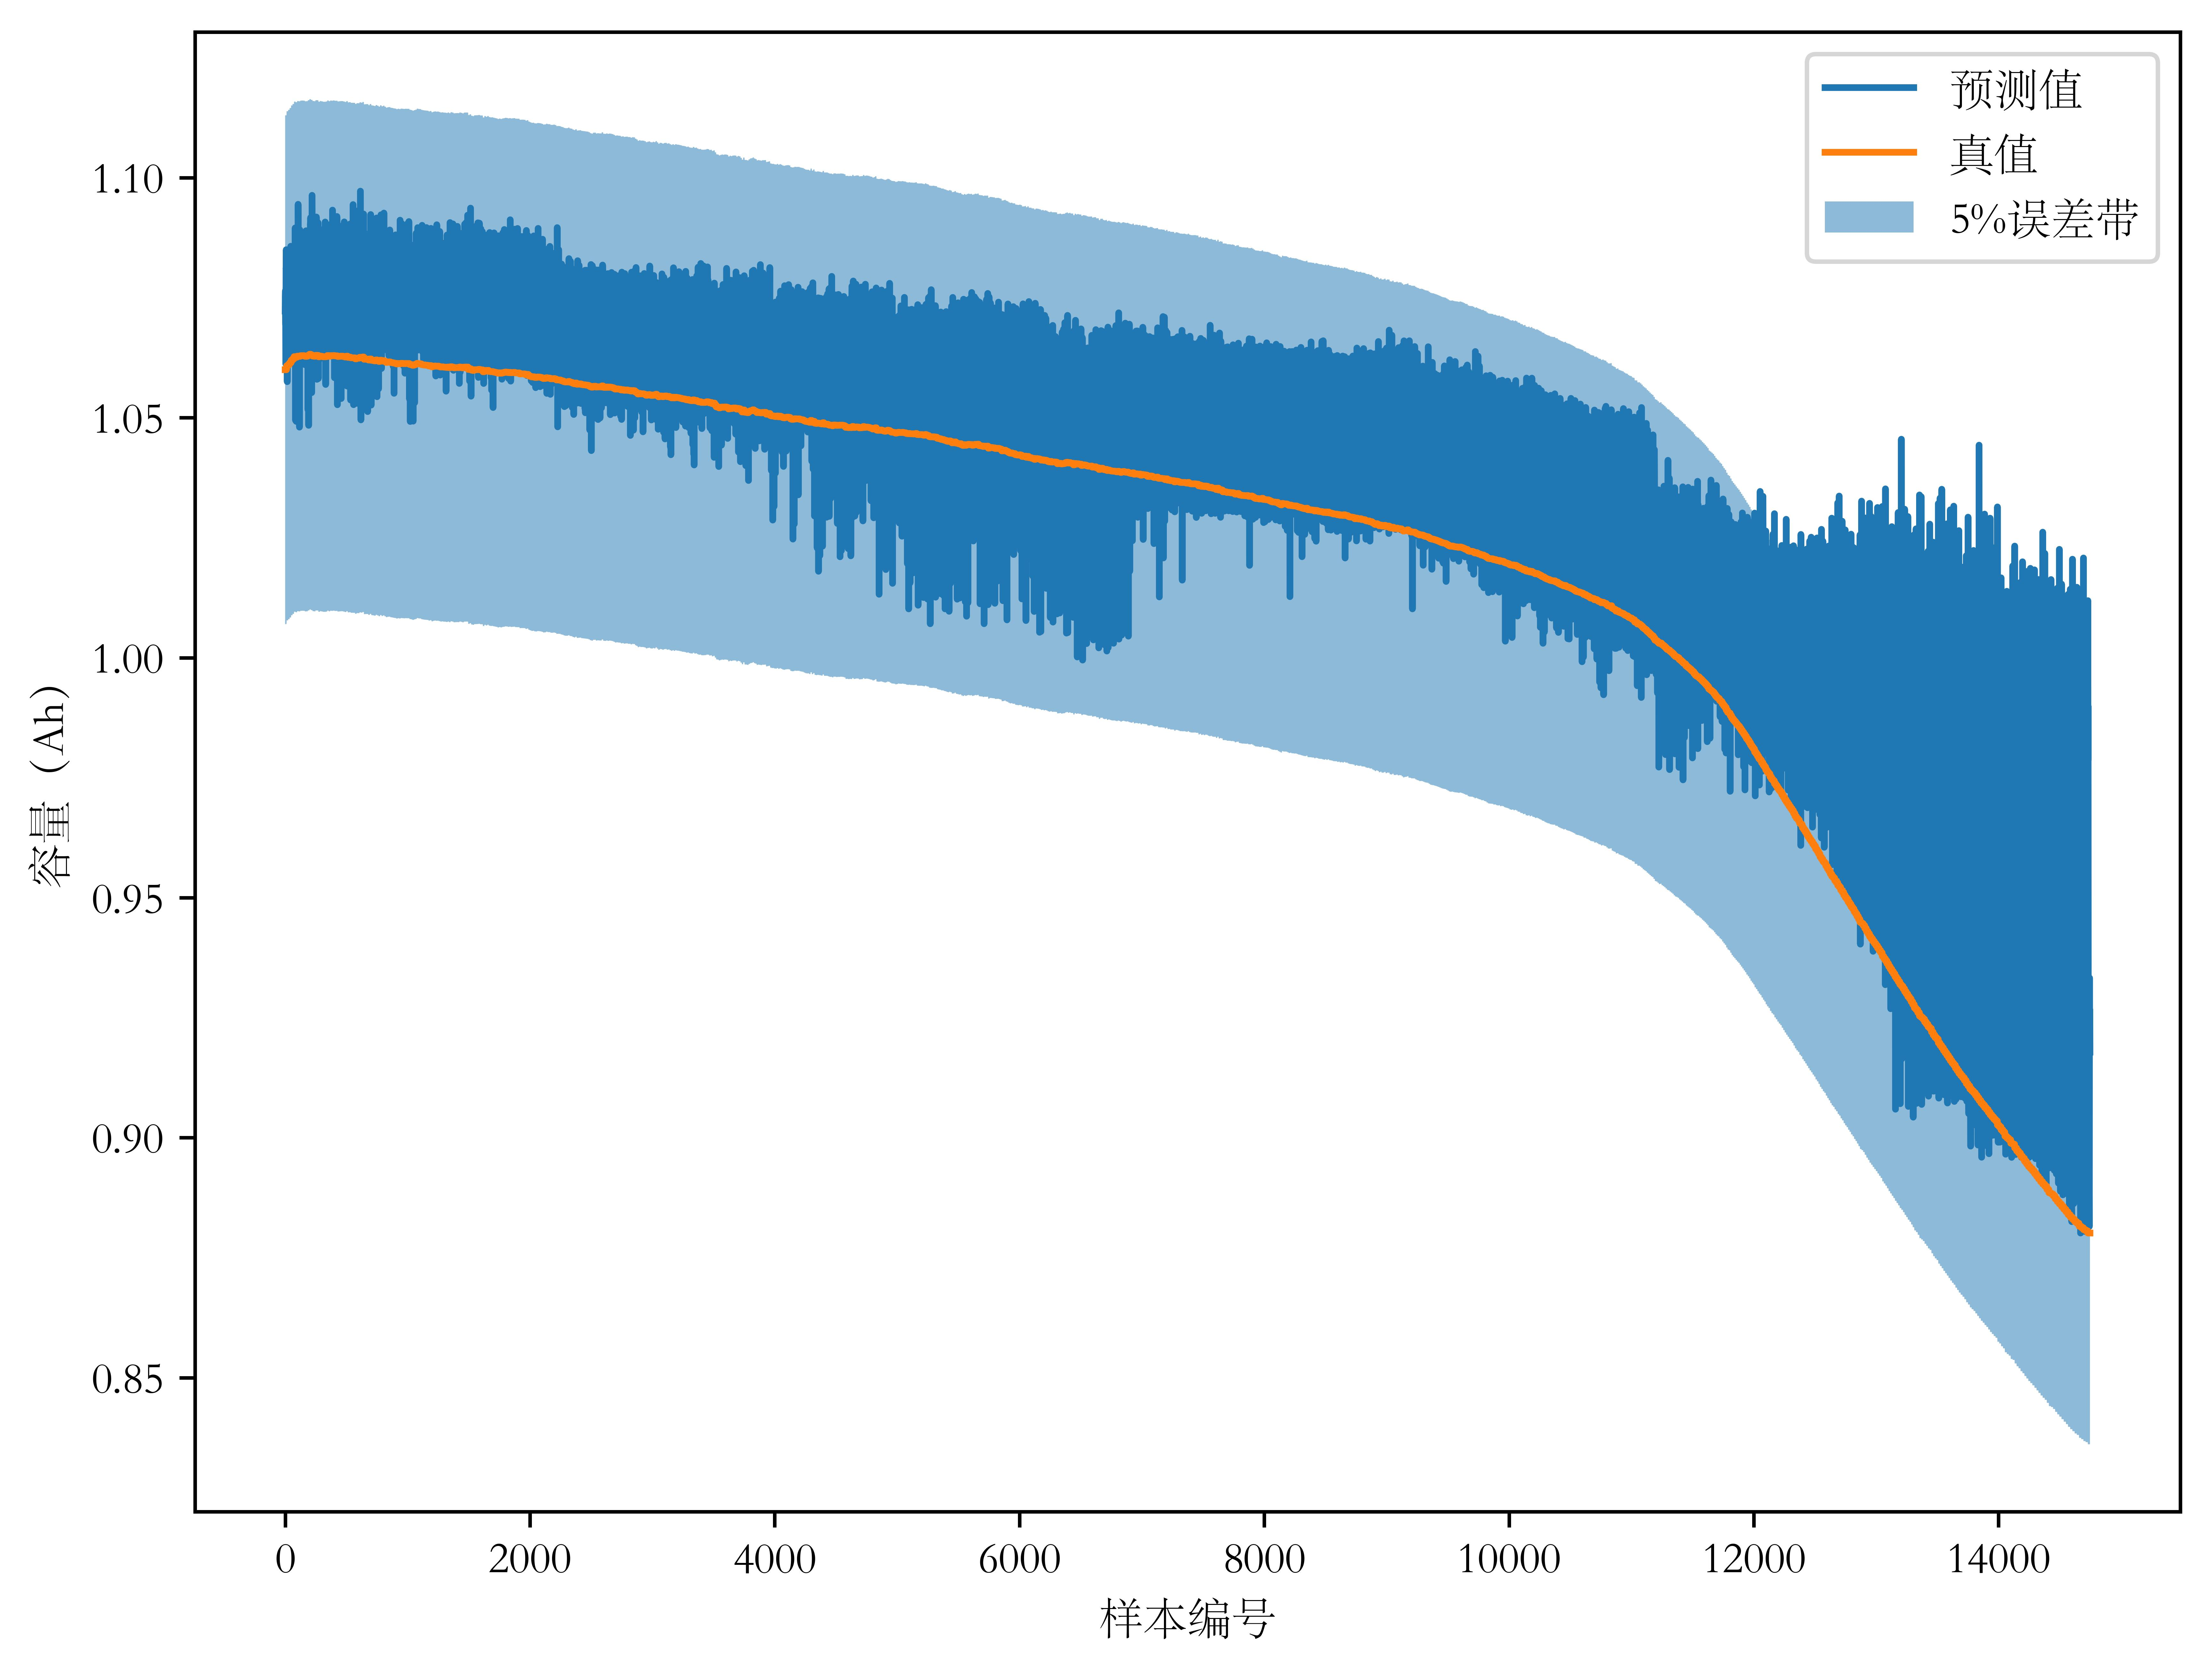
\includegraphics[width=0.2\textwidth]{figures/soh_vitq/tri_group1_cell3_cnn_vit_trans.jpg}}
			{\label{fig:subfig4}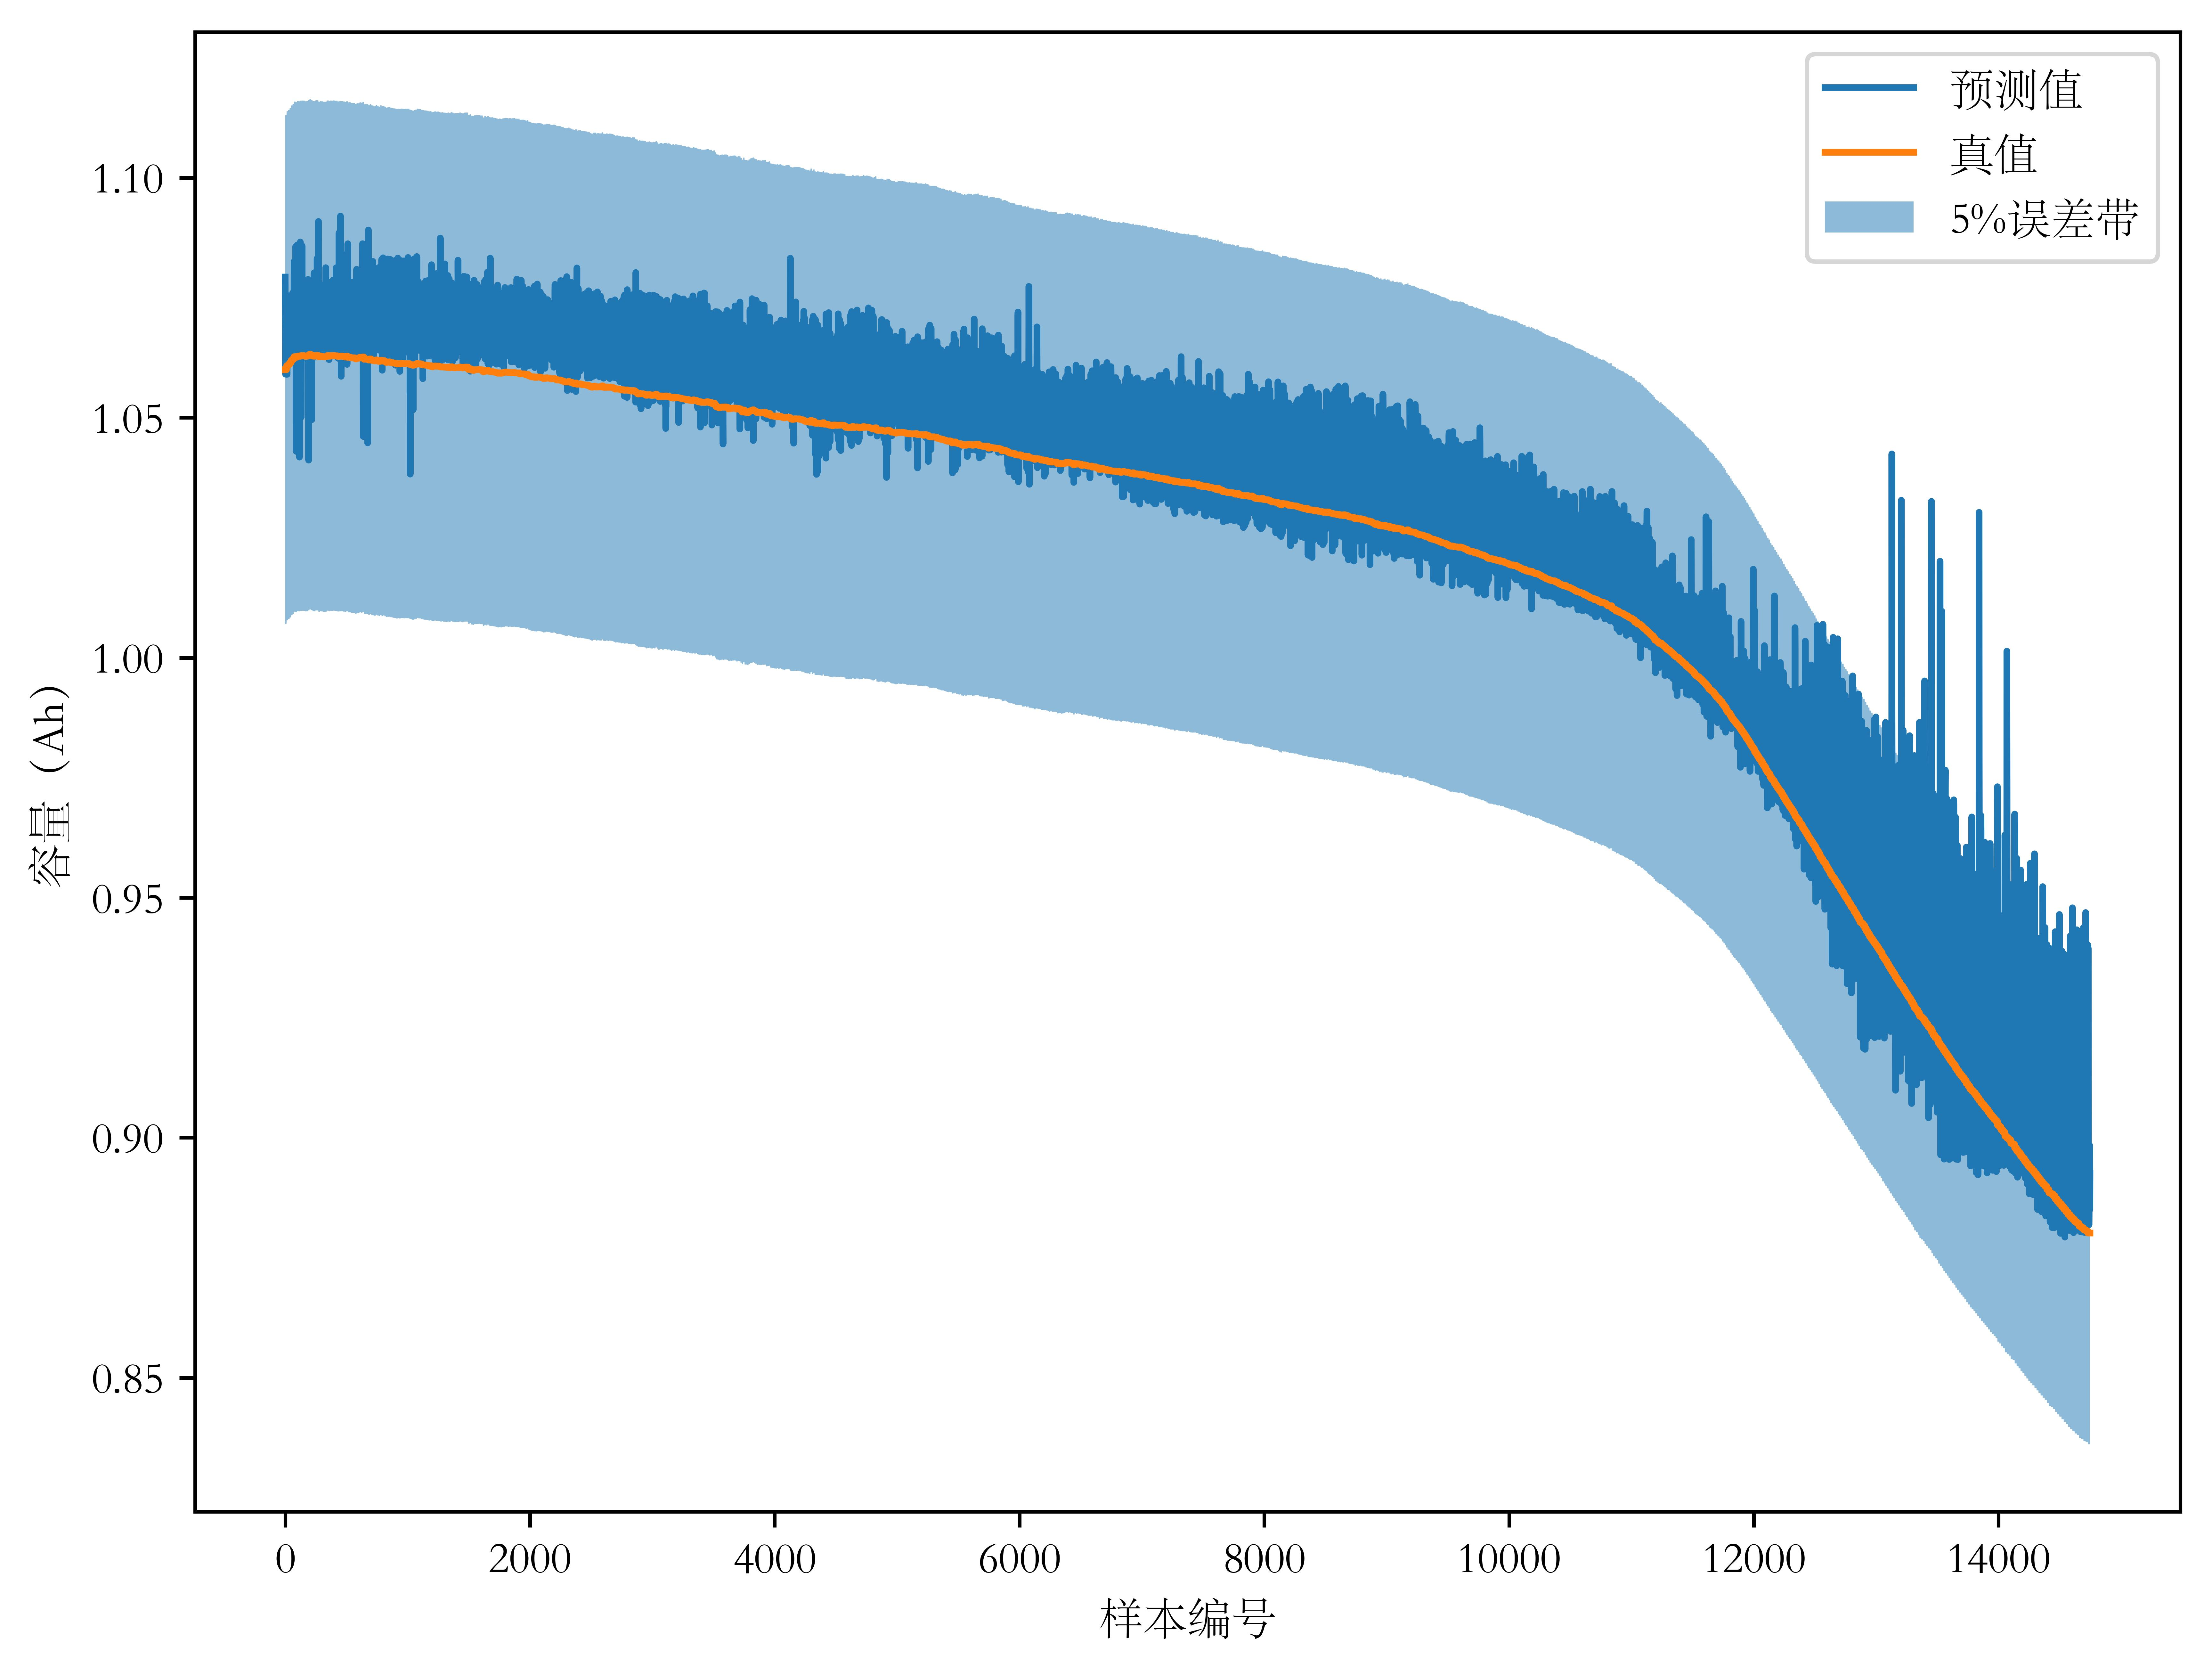
\includegraphics[width=0.2\textwidth]{figures/soh_vitq/tri_group1_cell3_cnn_viq_trans.jpg}}
	\end{figure}
	\begin{figure}[htbp]
		\centering
			{\label{fig:subfig1}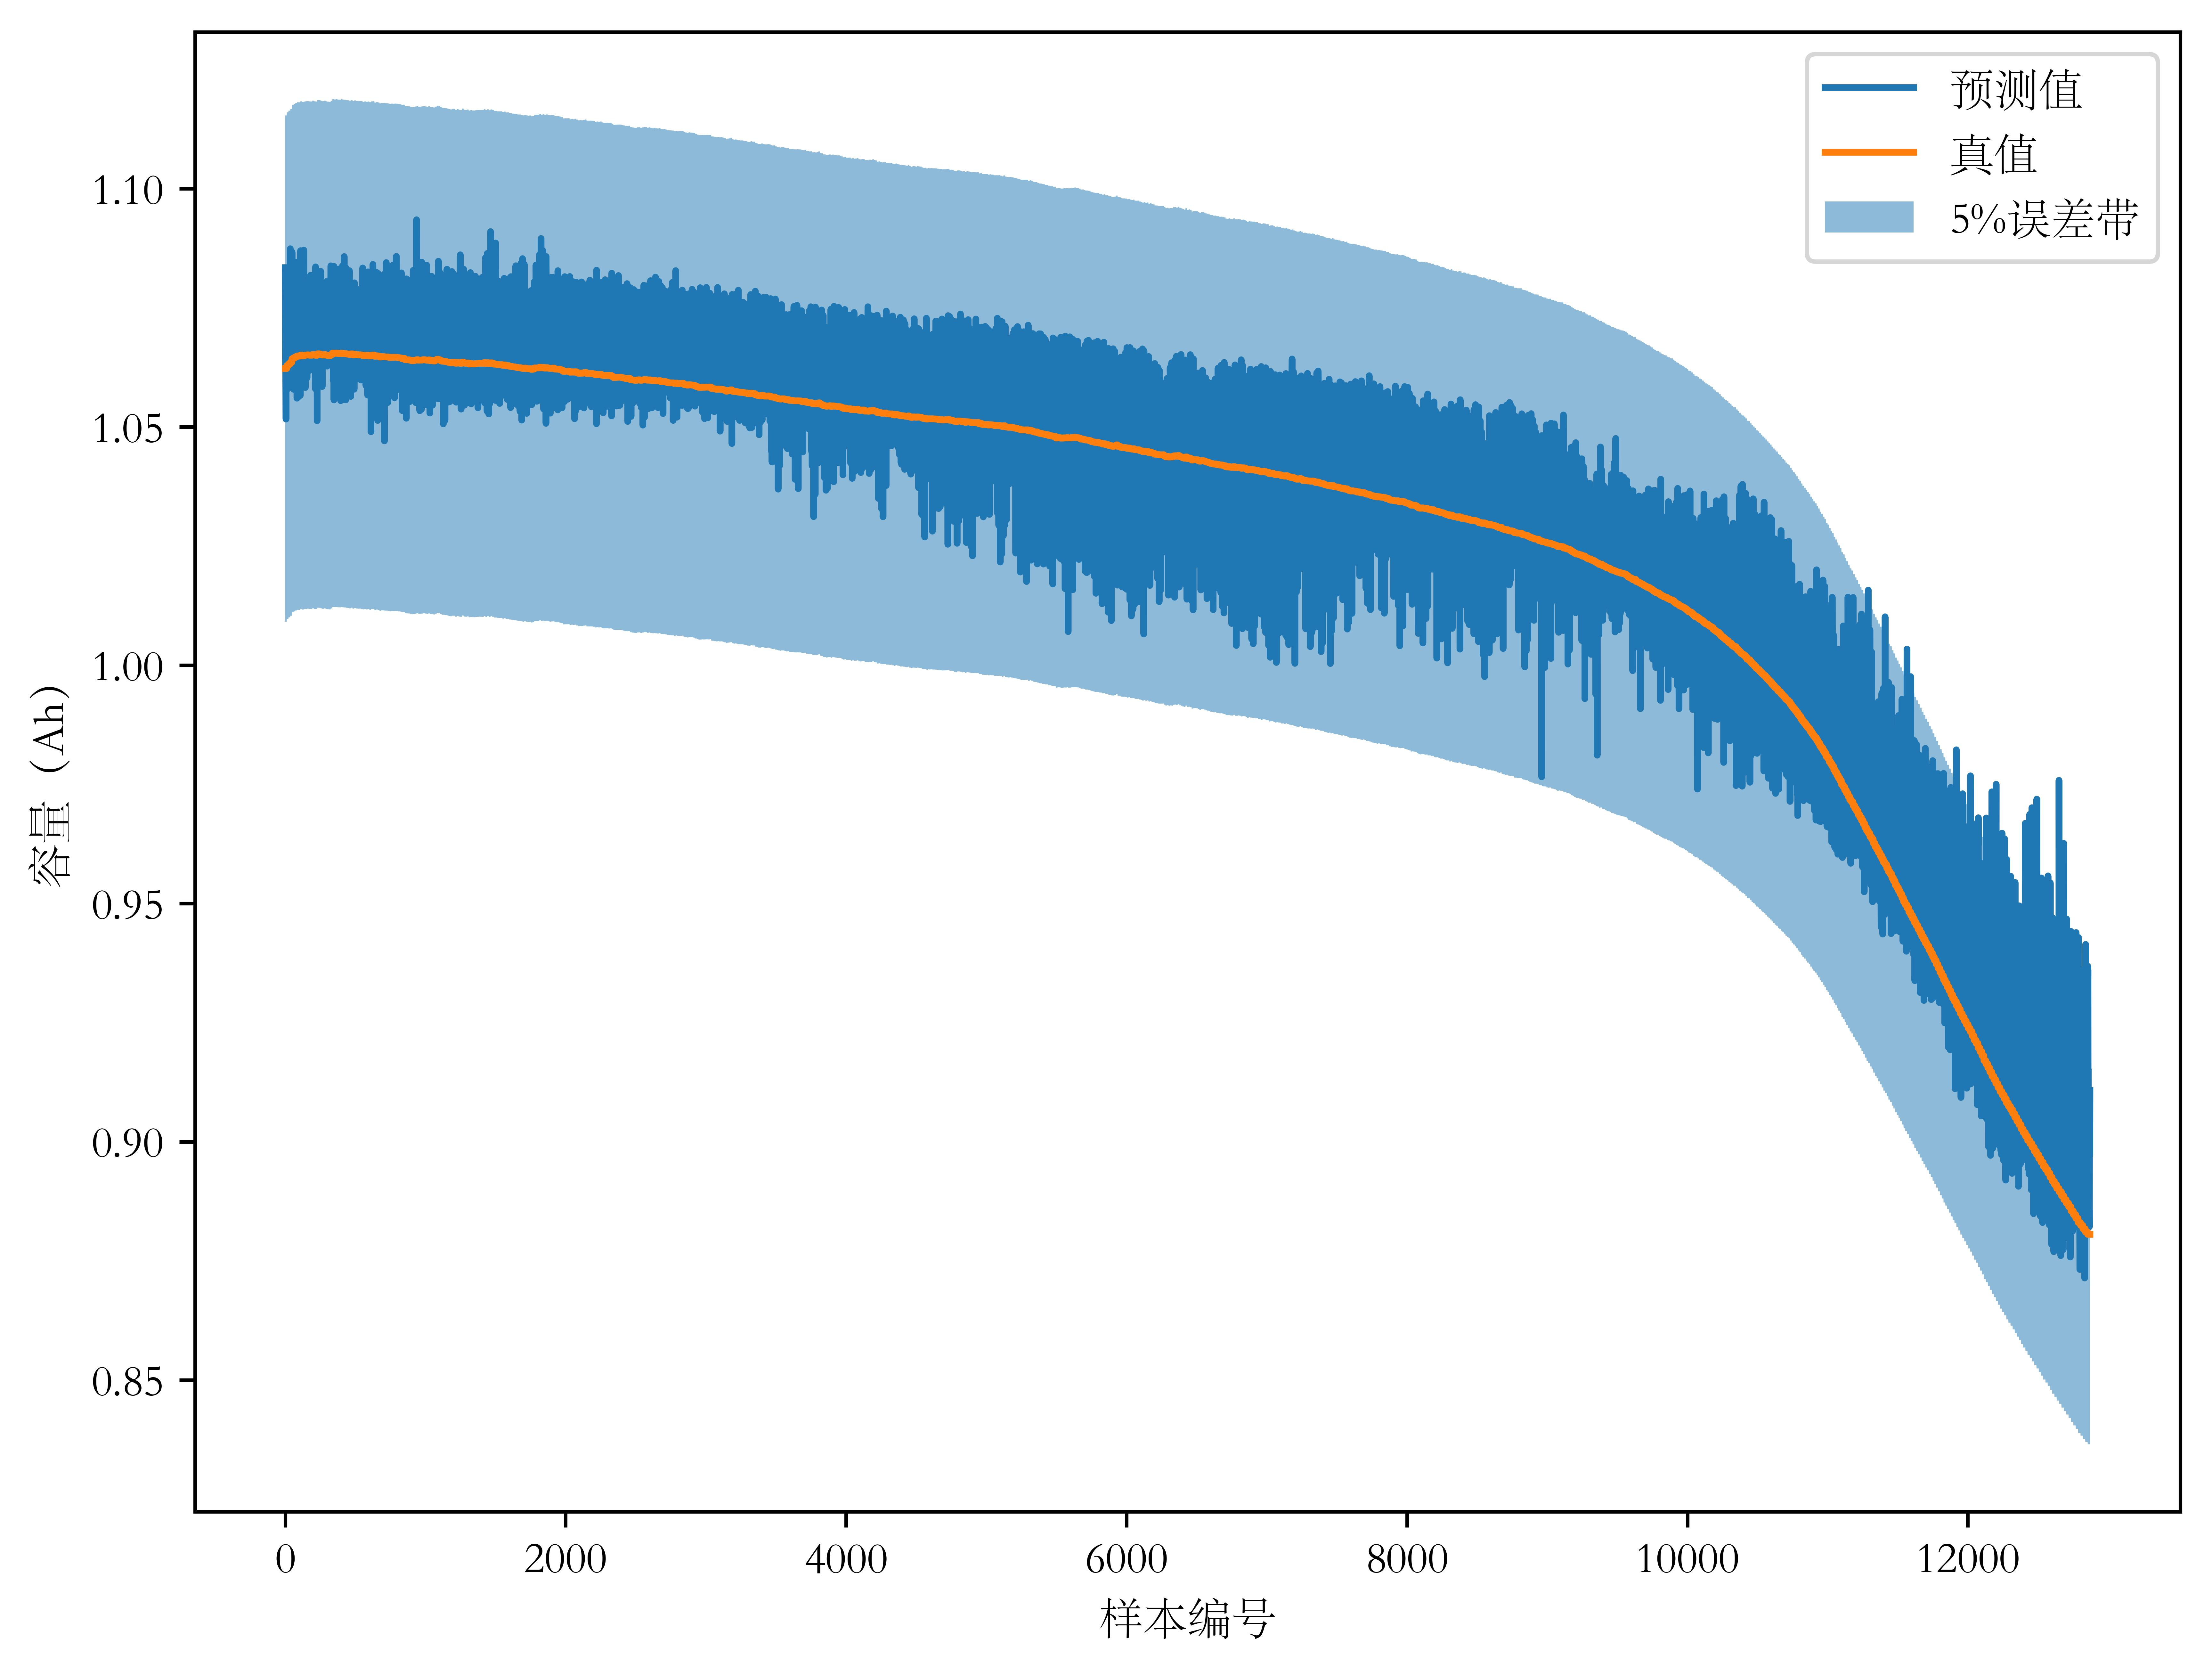
\includegraphics[width=0.2\textwidth]{figures/soh_vitq/tri_group1_cell4_cnn_vit.jpg}}
			{\label{fig:subfig2}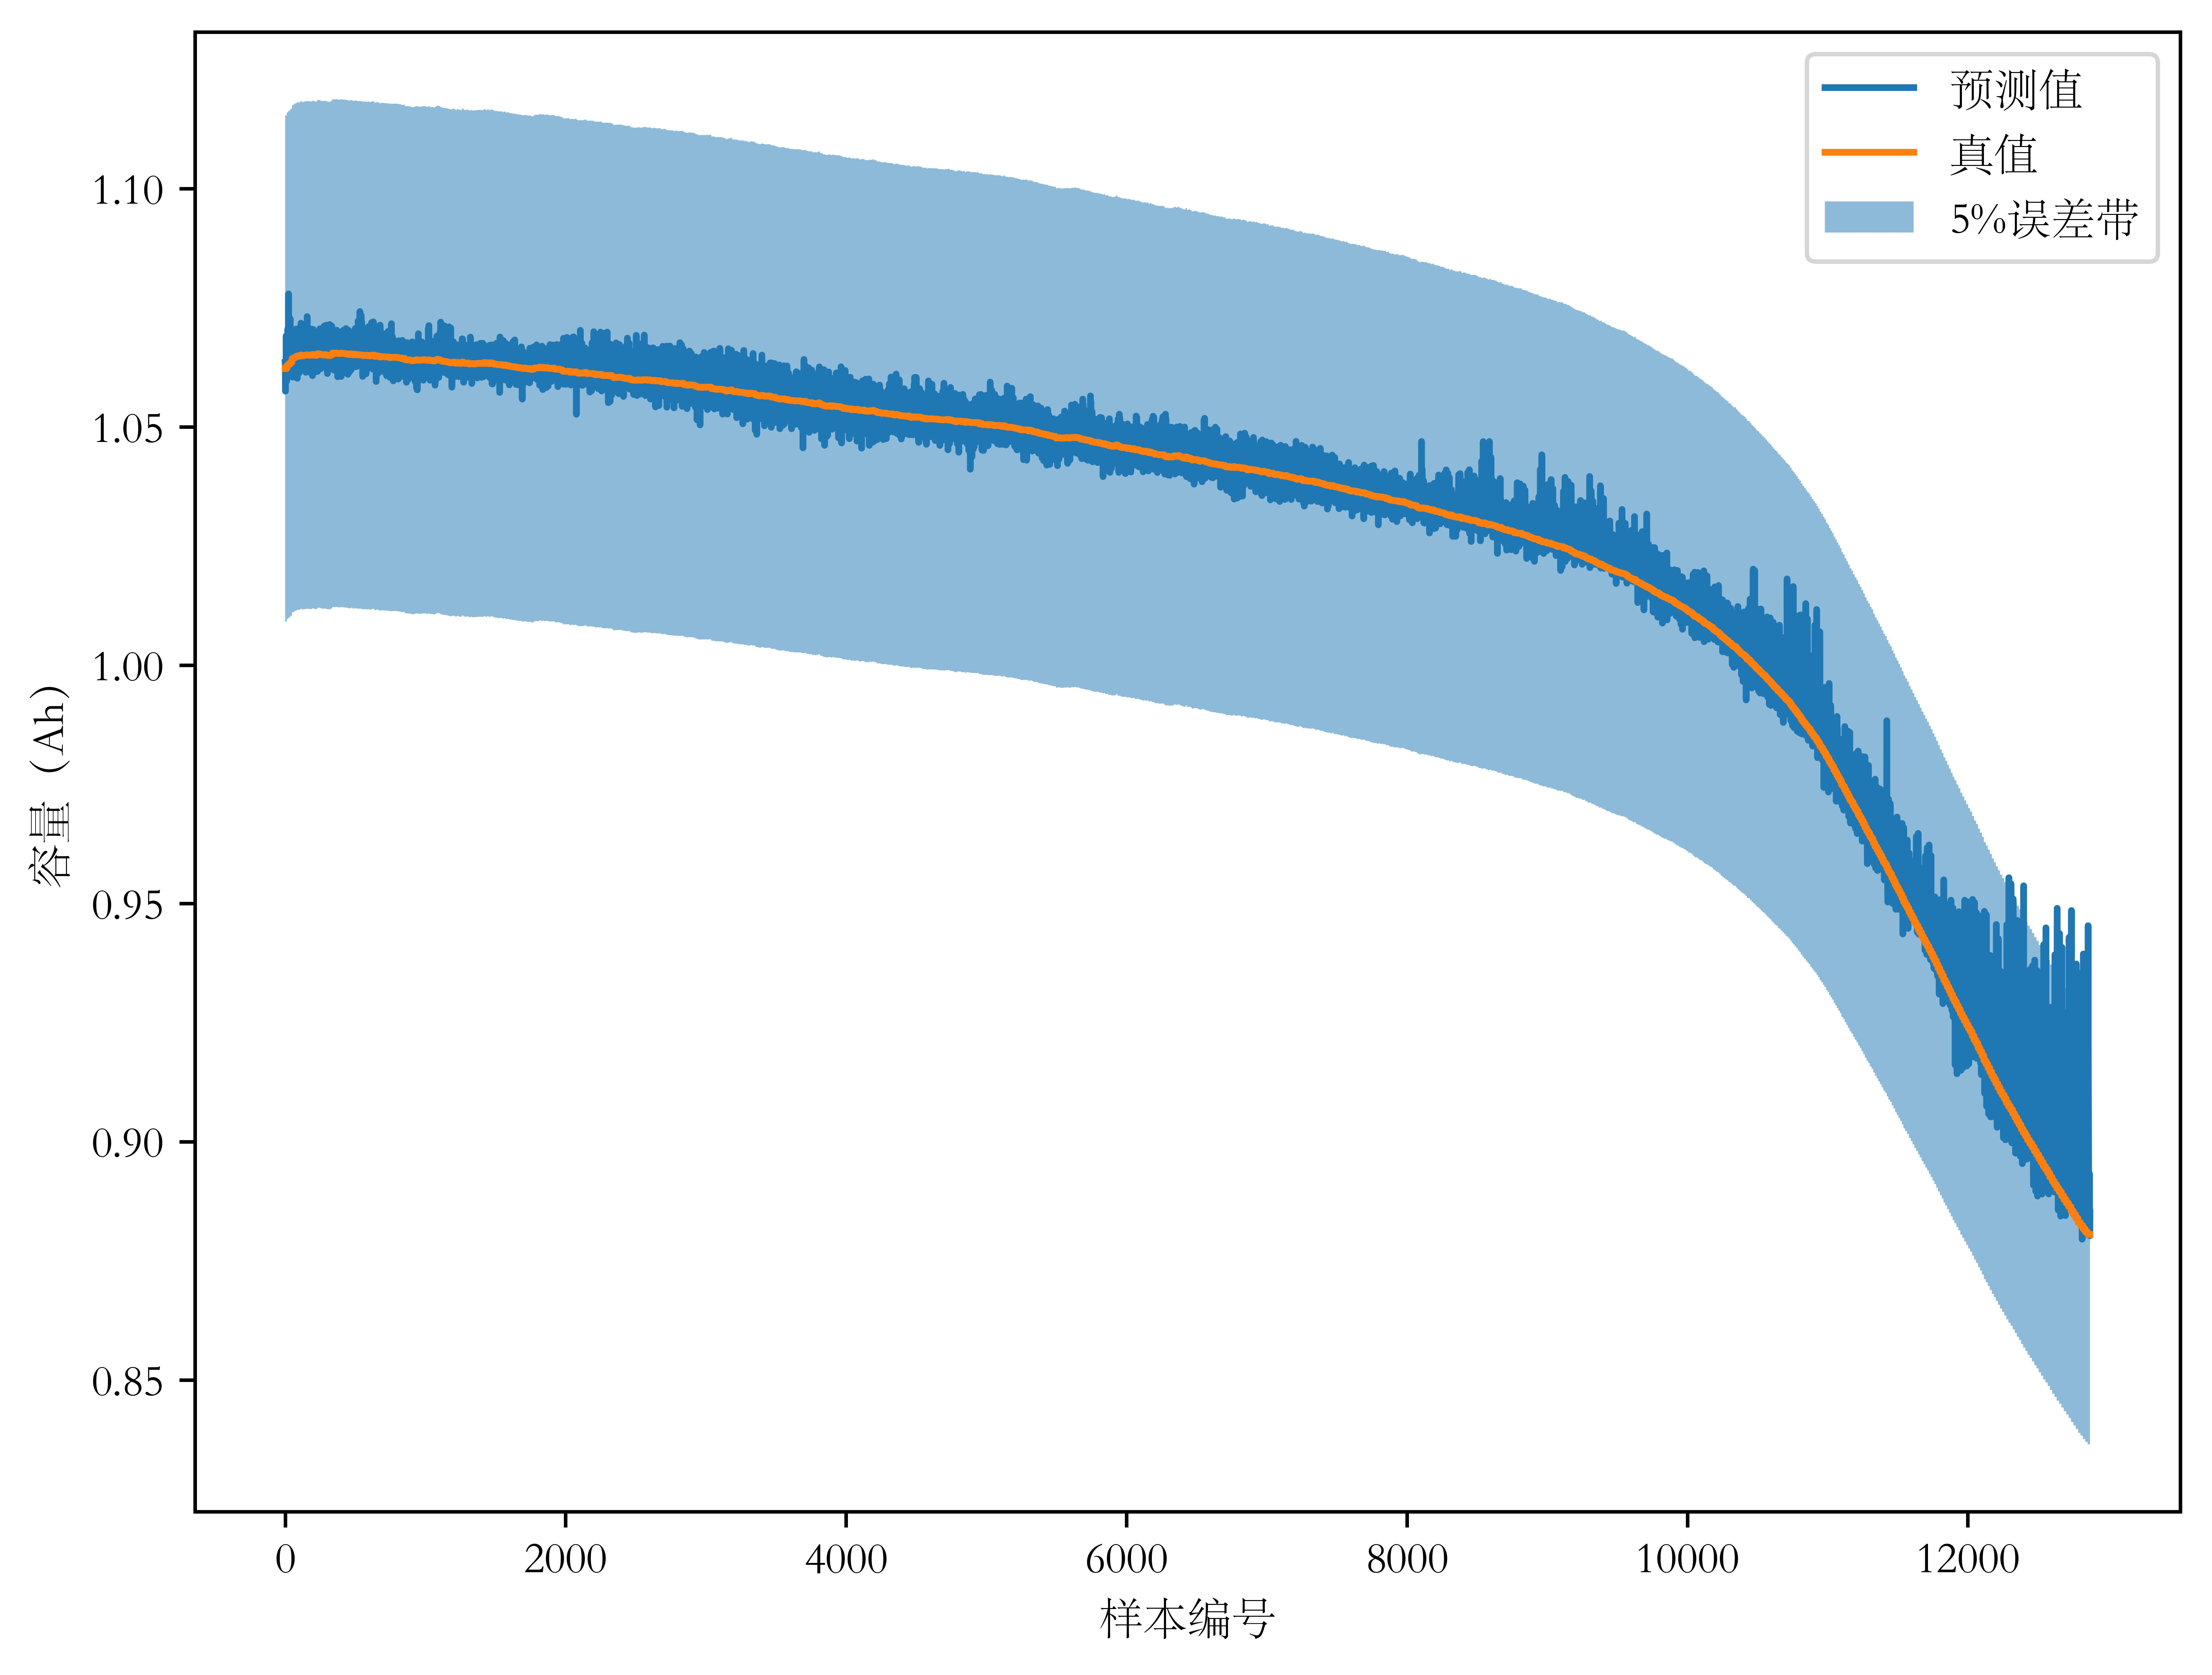
\includegraphics[width=0.2\textwidth]{figures/soh_vitq/tri_group1_cell4_cnn_viq.jpg}}
			{\label{fig:subfig3}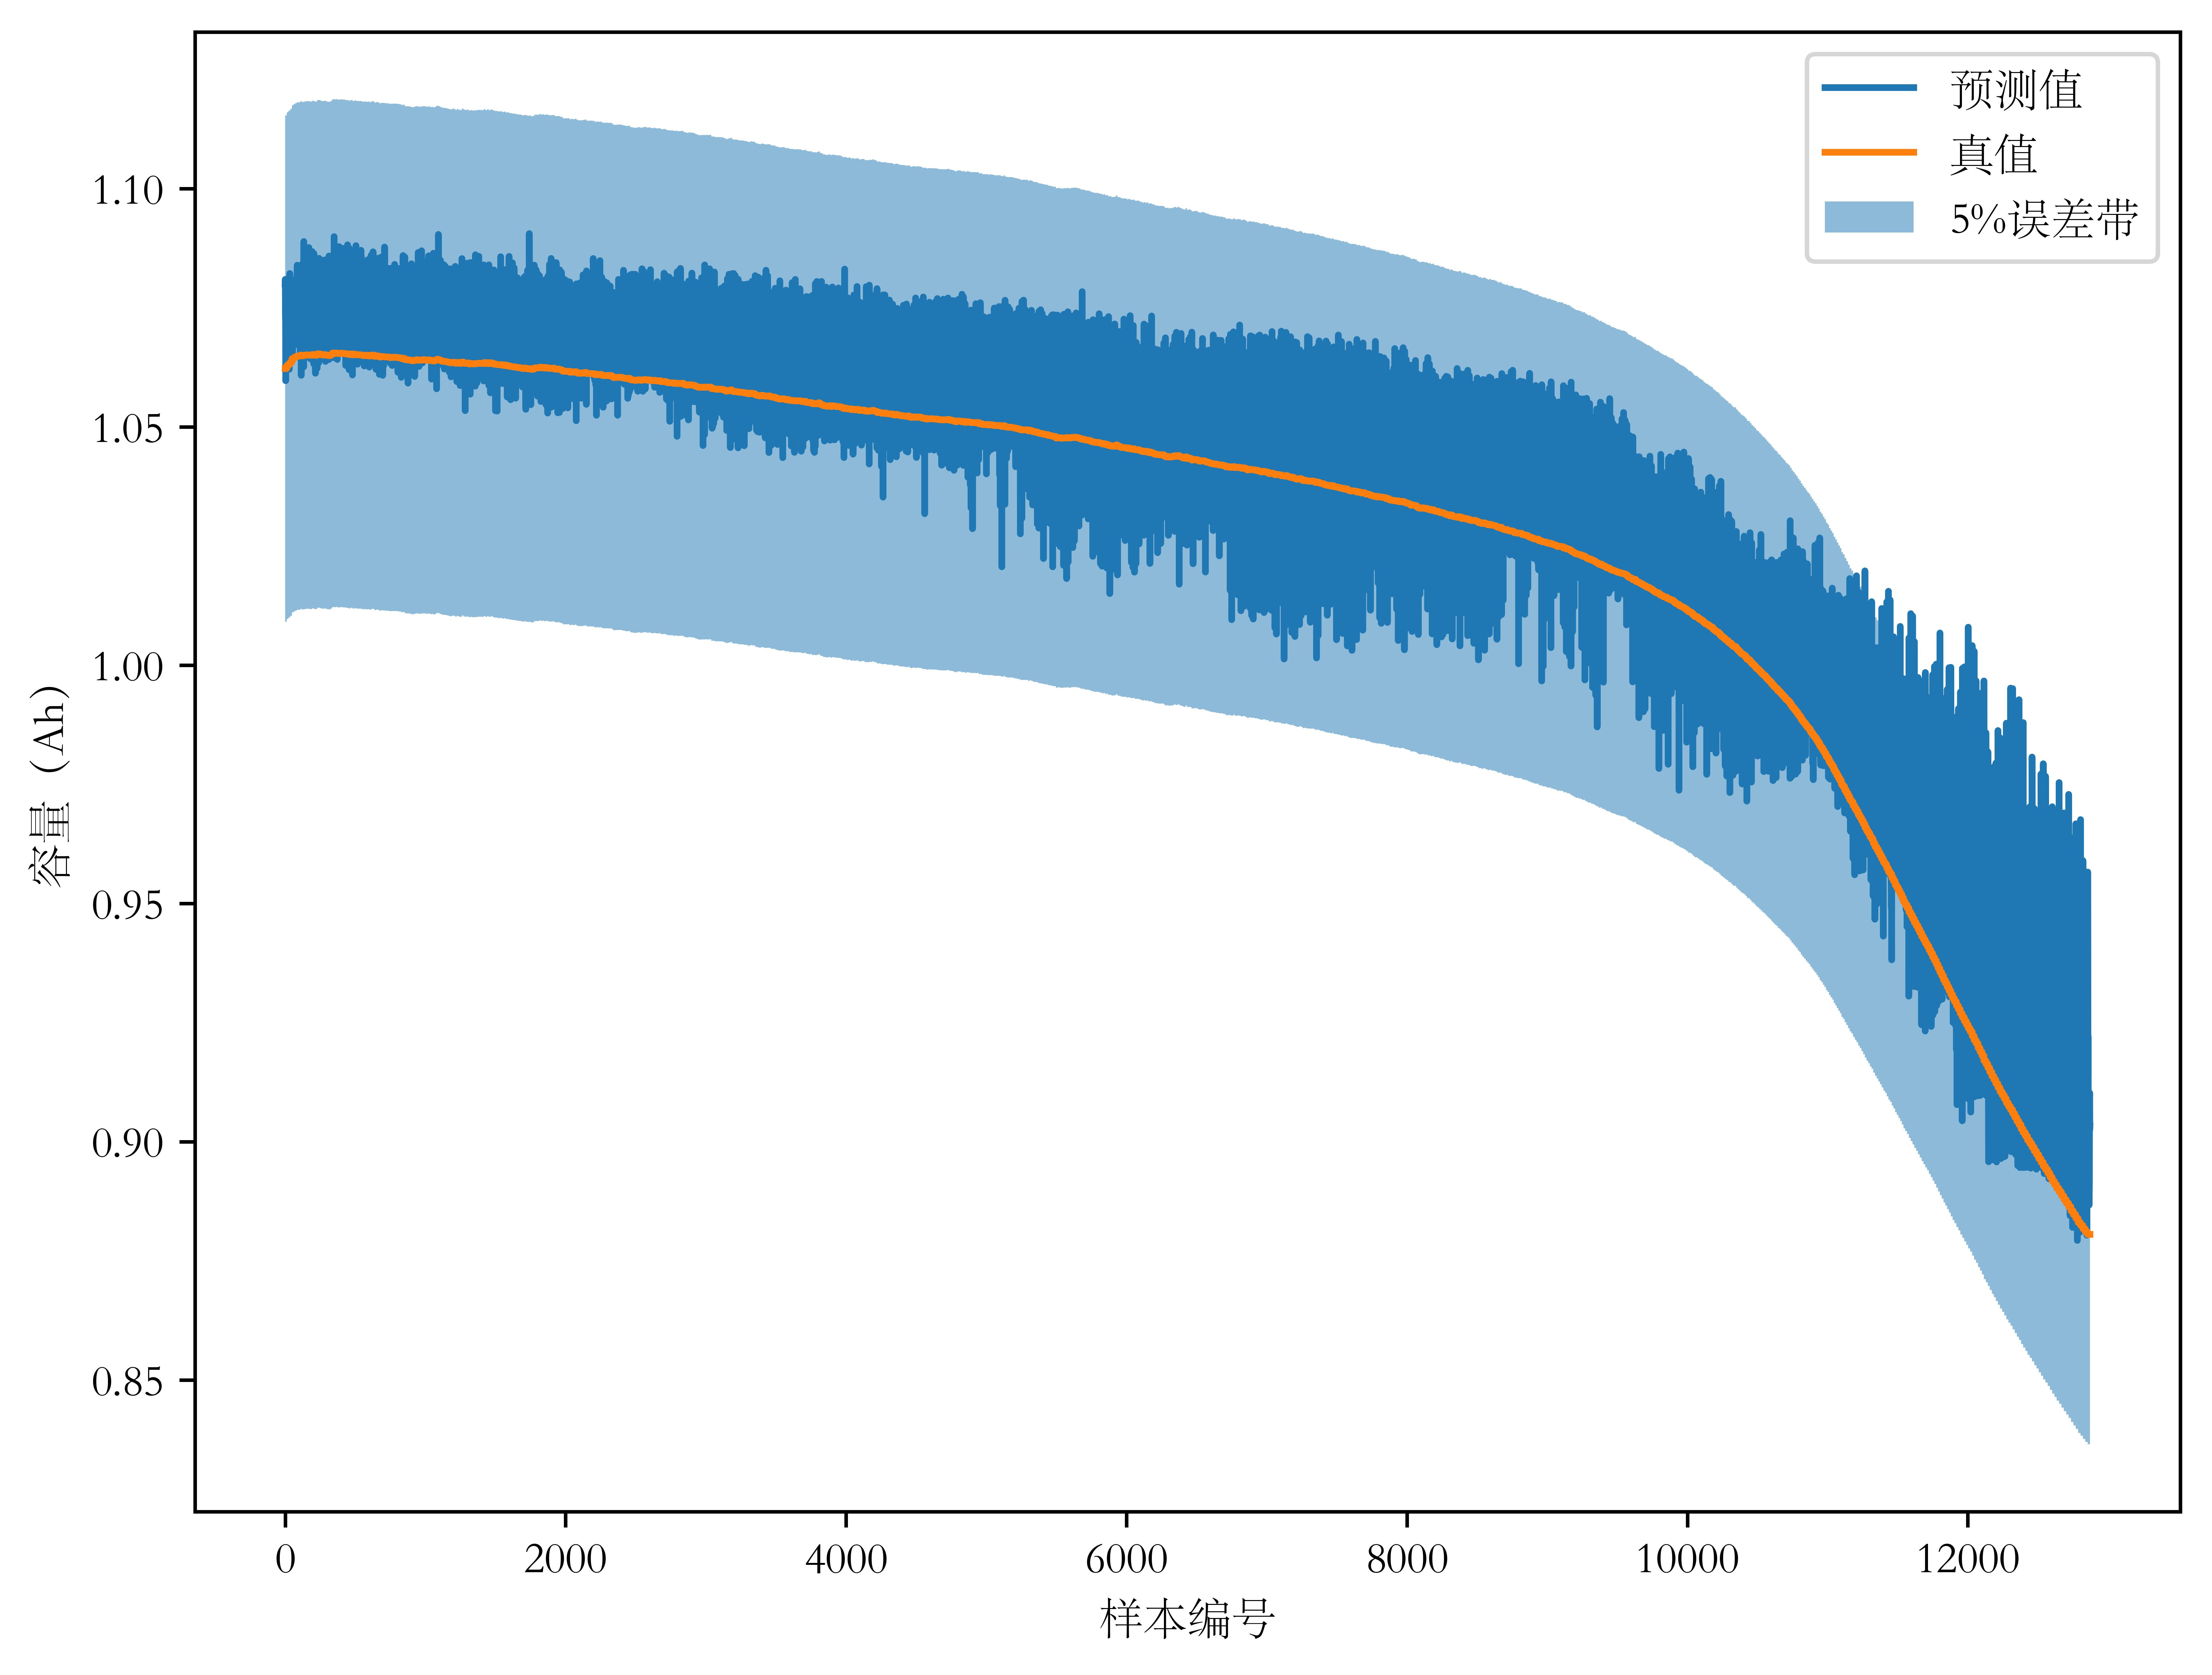
\includegraphics[width=0.2\textwidth]{figures/soh_vitq/tri_group1_cell4_cnn_vit_trans.jpg}}
			{\label{fig:subfig4}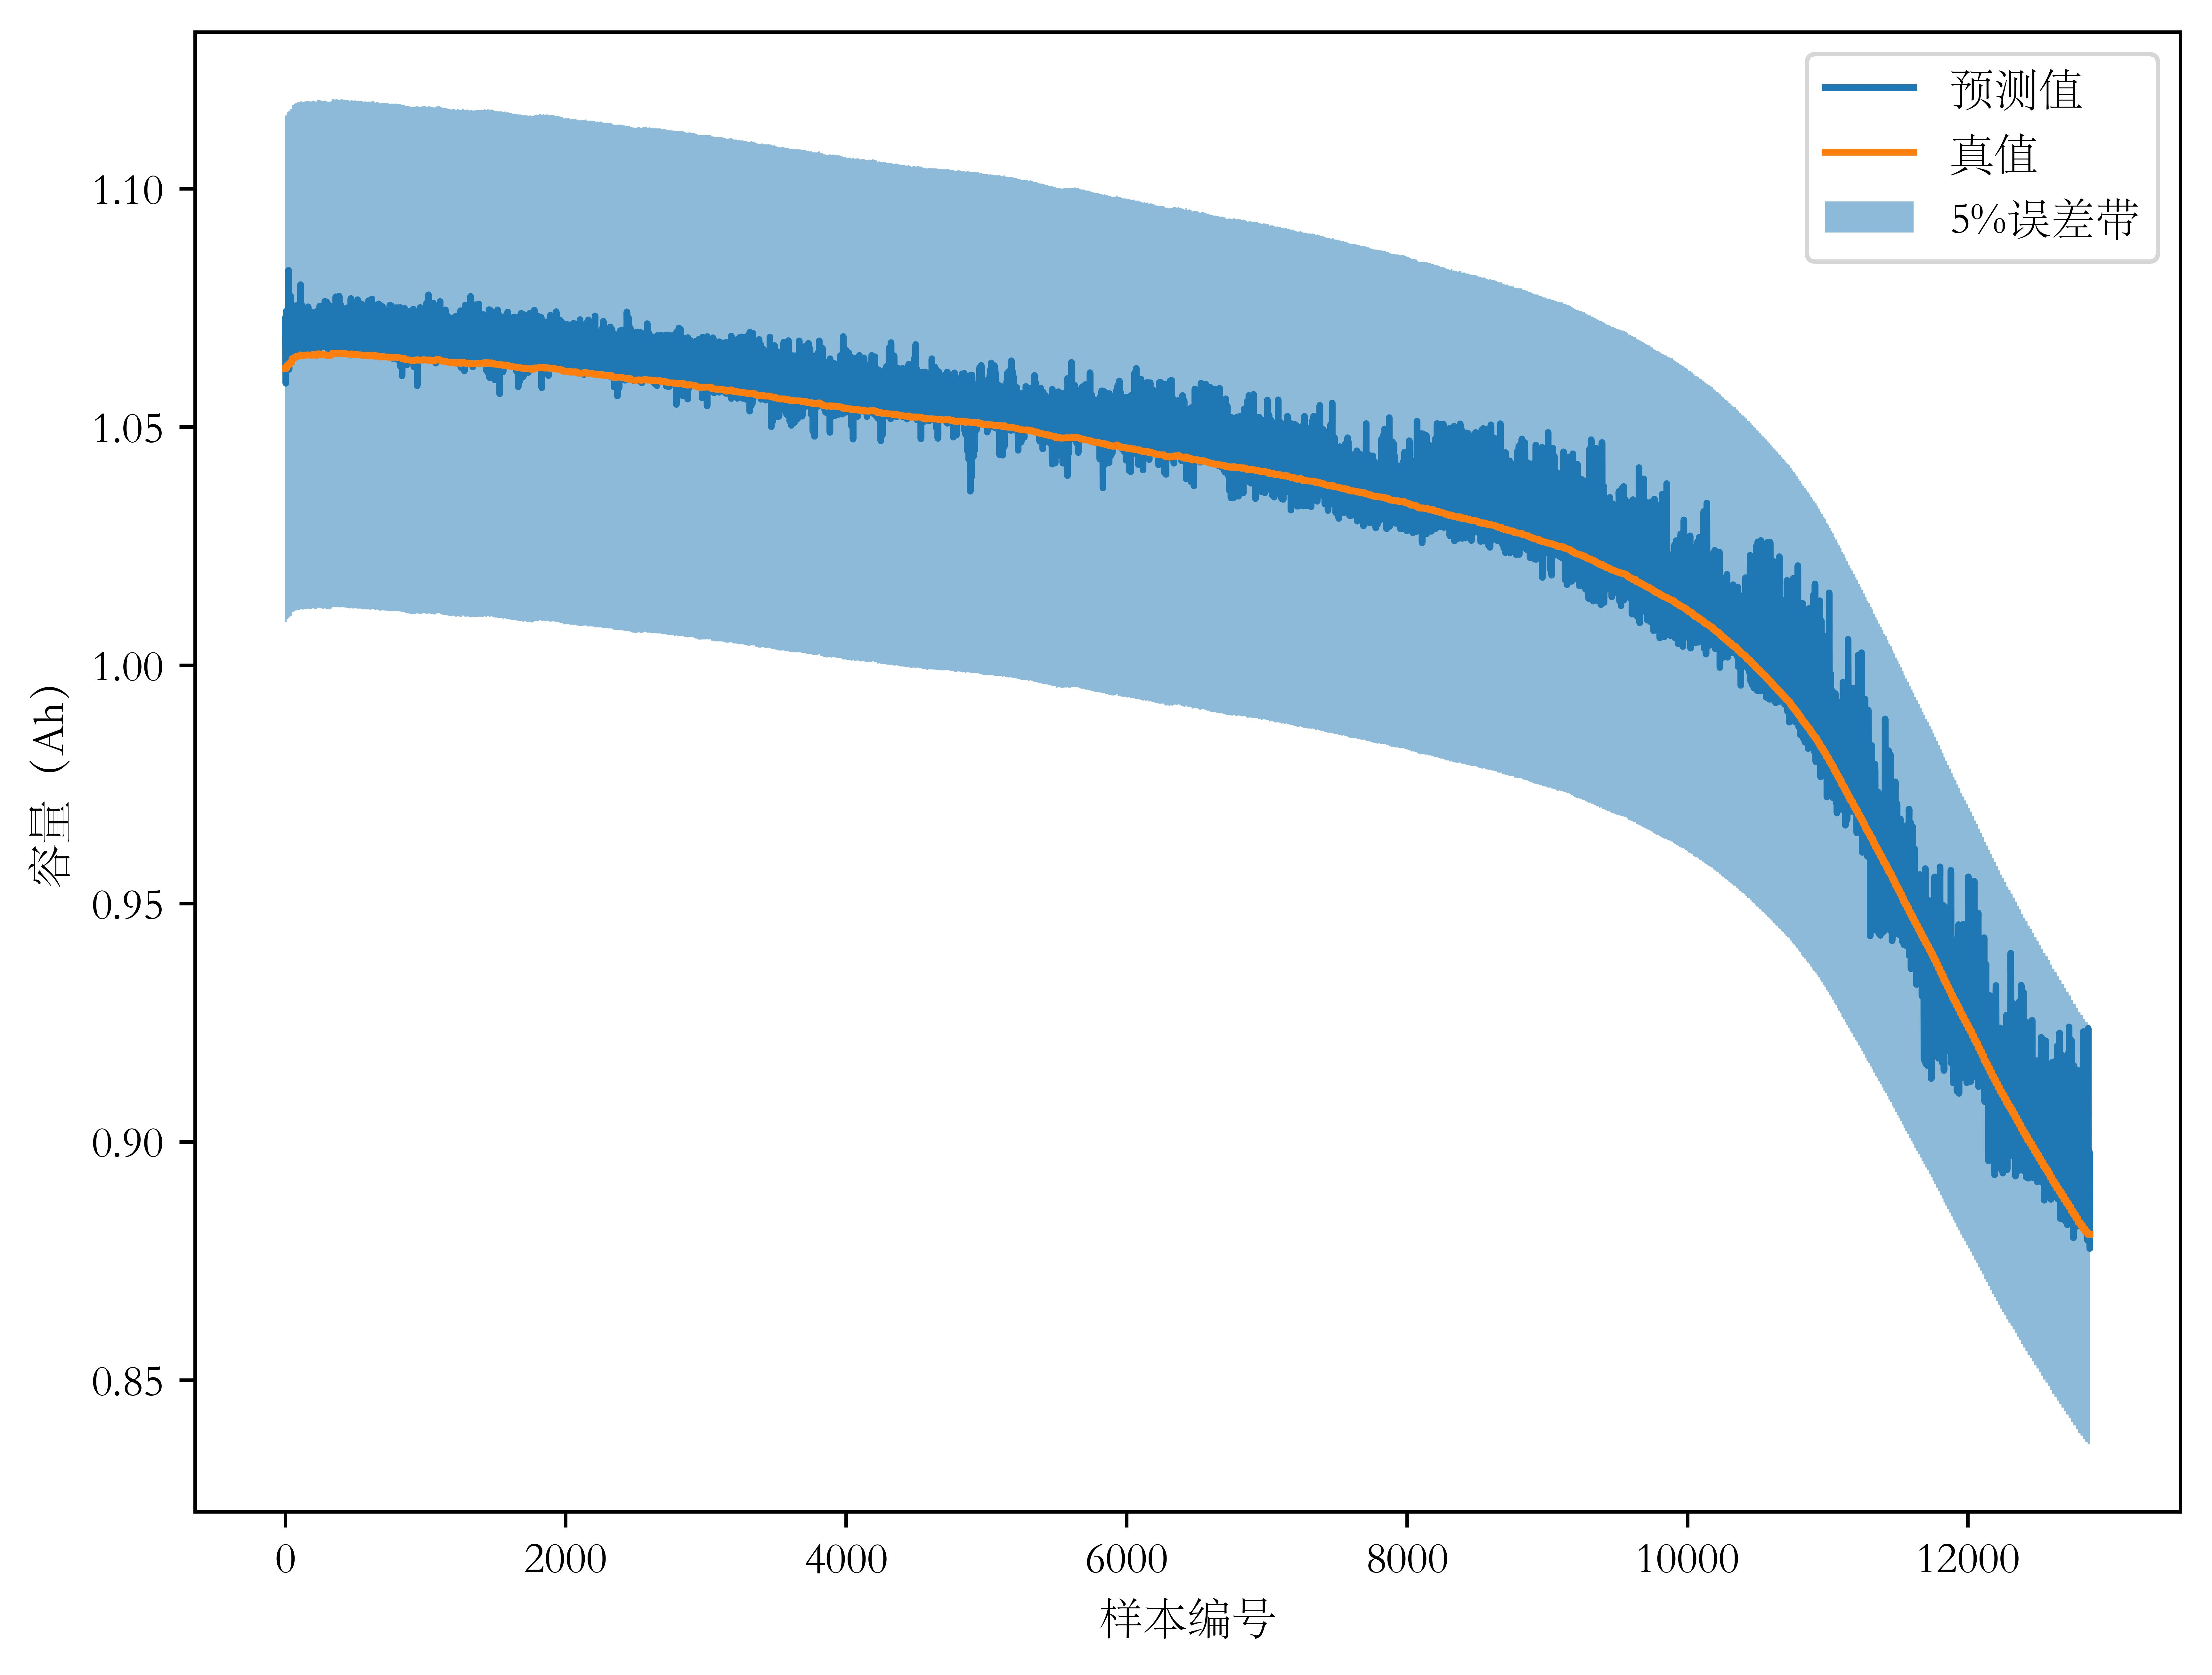
\includegraphics[width=0.2\textwidth]{figures/soh_vitq/tri_group1_cell4_cnn_viq_trans.jpg}}
	\end{figure}
\end{frame}

\begin{frame}
\begin{table}[]
	\centering
	\resizebox{\columnwidth}{!}{%
	\begin{tabular}{ccccc}
	\toprule
	评价指标   & 第一组实验    & 第二组实验    & 第三组实验    & 第四组实验    \\
	\midrule
	平均MaxE & 0.110514 & 0.131351 & 0.08509  & 0.068284 \\
	平均MAE  & 0.011018 & 0.015671 & 0.006605 & 0.006807 \\
	平均RMSE & 0.016167 & 0.021842 & 0.010835 & 0.009845 \\
	模型参数量  & 60421    & 12693    & 60421    & 12693   \\
	\bottomrule
	\end{tabular}%
	}
	\caption{四组实验CNN模型预测性能评估结果}
	\end{table}
	\begin{itemize}
		\item 对比使用V、I、T为输入的情形,使用V、I、q为输入时模型预测结果有很大提升
		\item 使用时间序列-图像变换能在保持预测精度的前提下显著降低模型参数量
	\end{itemize}
\end{frame}

\subsection{电池RUL预测}

\begin{frame}
	\begin{itemize}
		\item 基于循环圈数定义的RUL(cycle-RUL)\\${RUL_{cycle} = n_{EOL} - n_{cycle}}$
		\item 基于容量定义的RUL(Ah-RUL)\\${RUL_{Ah} = \frac{trapz(M_{current}[:, :], M_{time}[:, :]) - trapz(M_{current}[n:EOL, :], M_{time}[n:EOL, :])}{C_{norm}}}$
	\end{itemize}
	\begin{figure}[htbp]
		\centering
			{\label{fig:subfig1}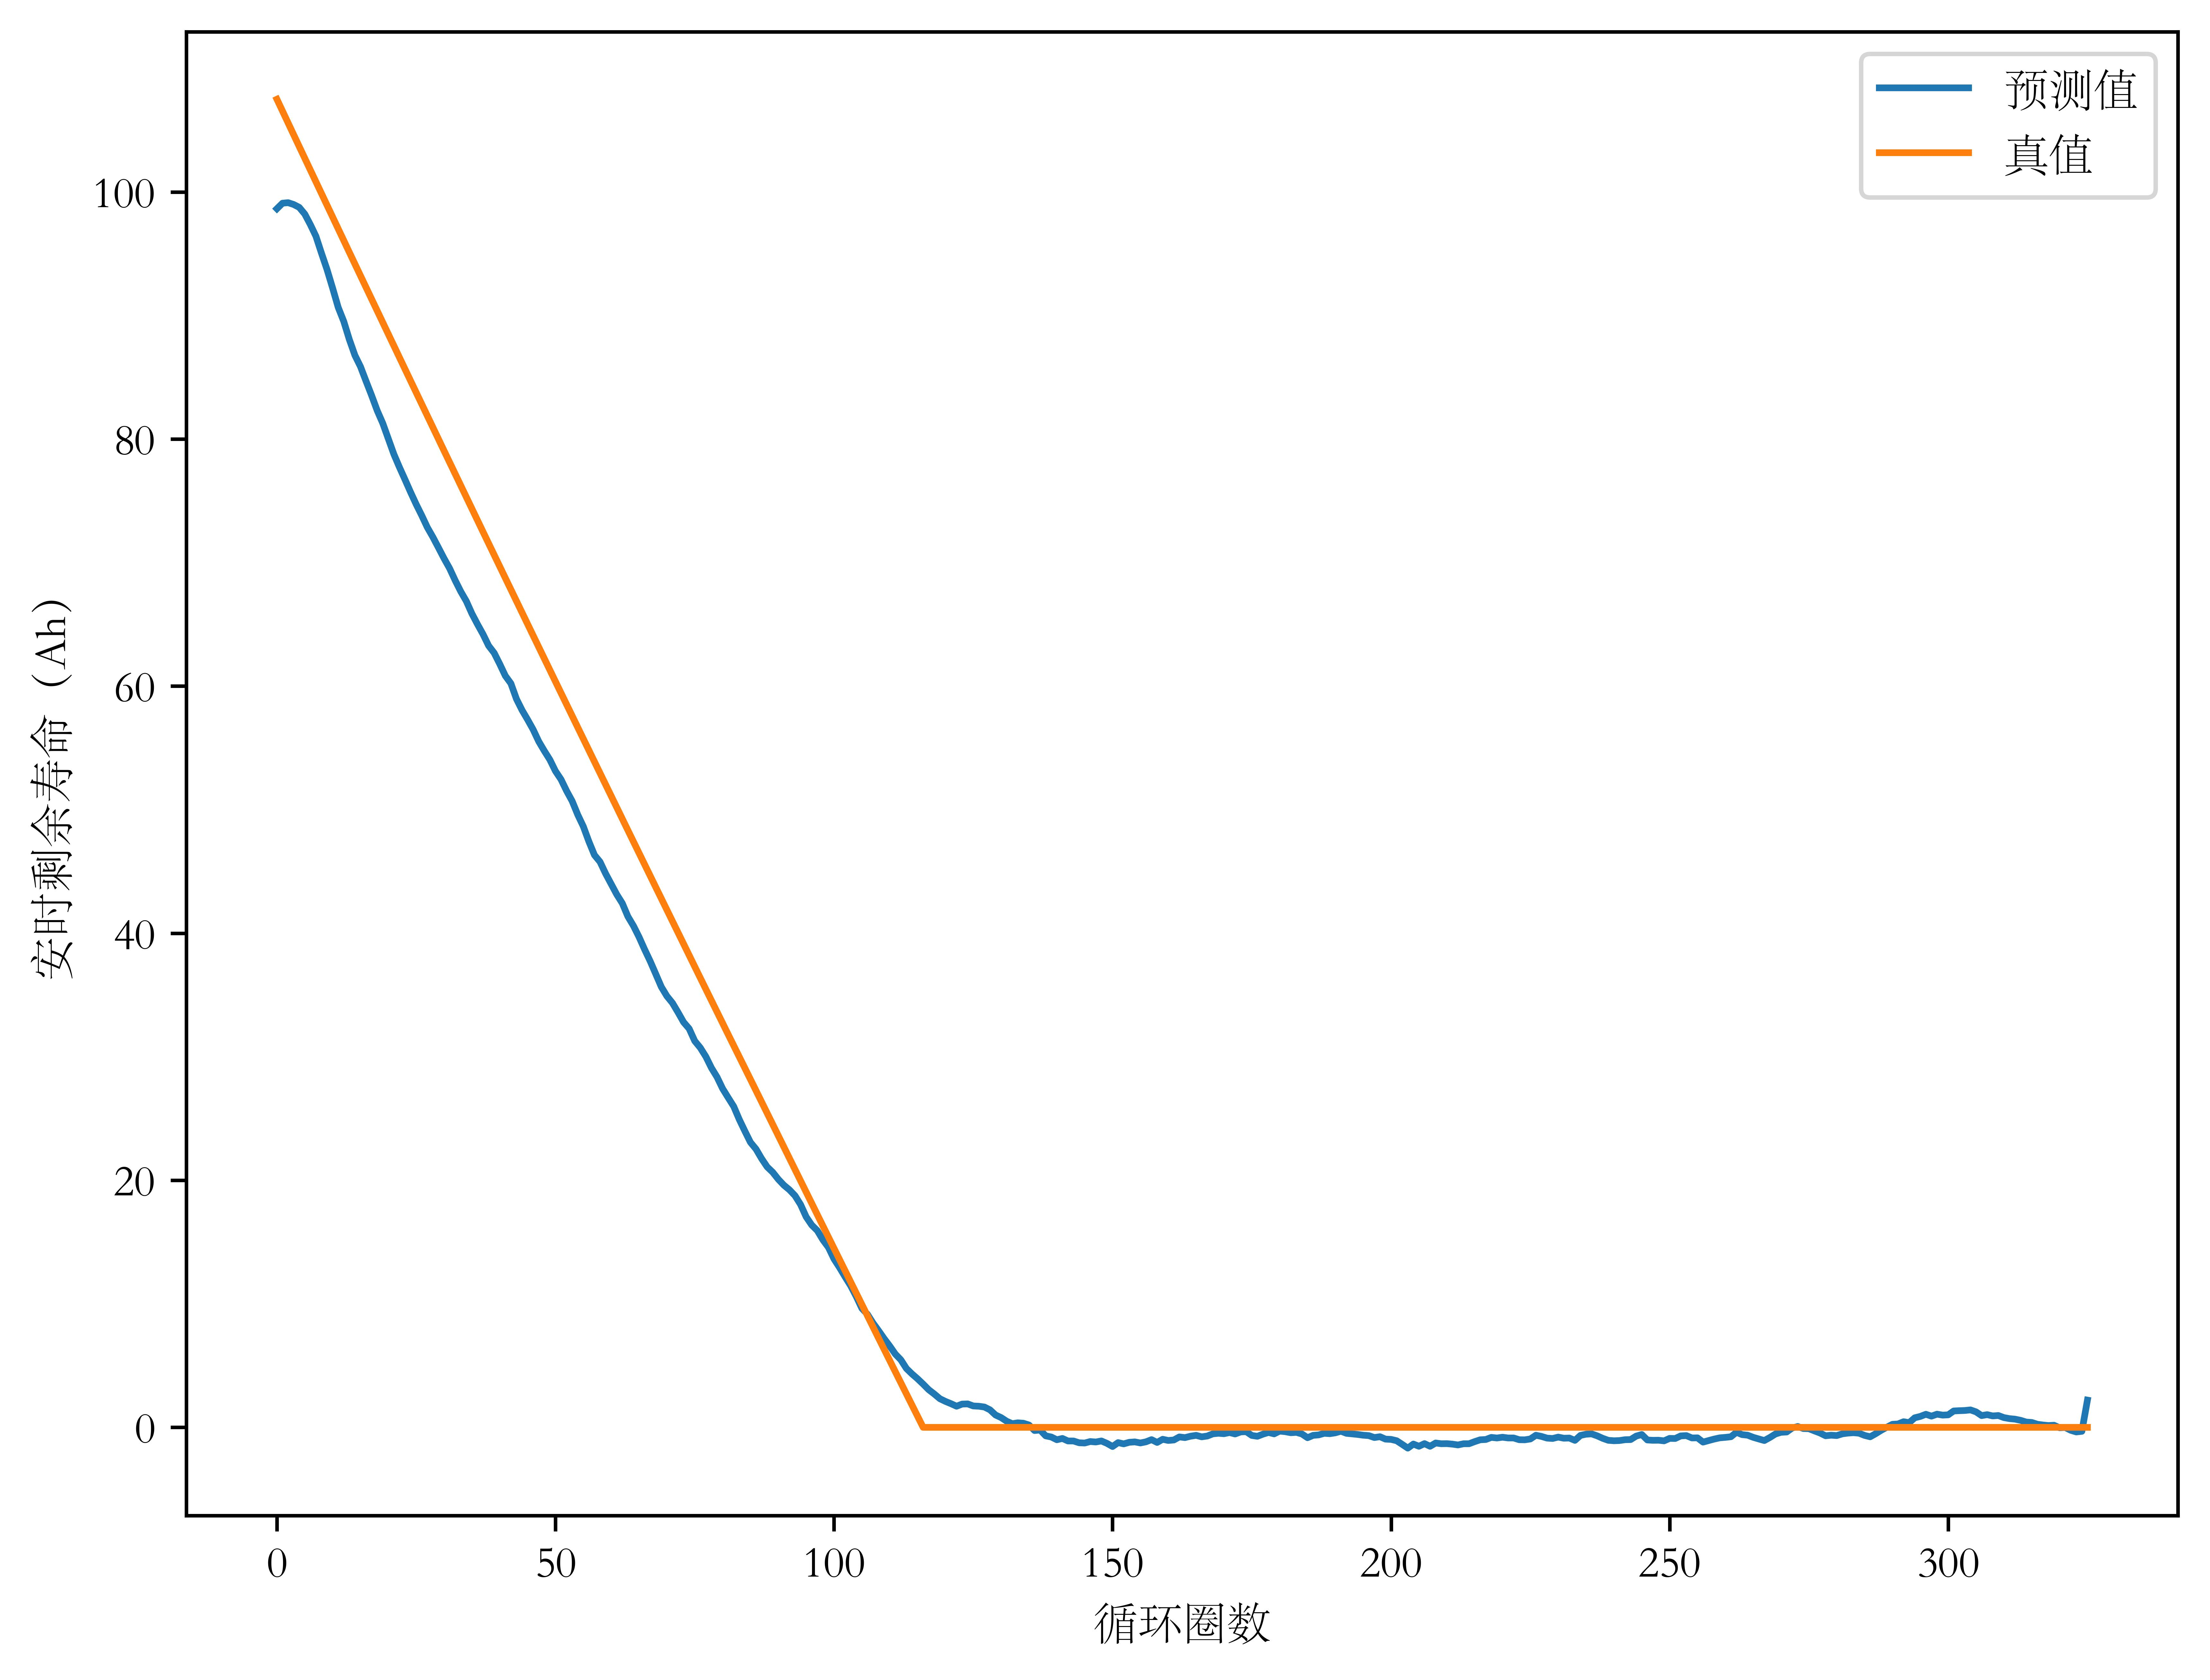
\includegraphics[width=0.3\textwidth]{figures/rul/unibo_lstm_rul_cycle_1.jpg}}
			{\label{fig:subfig2}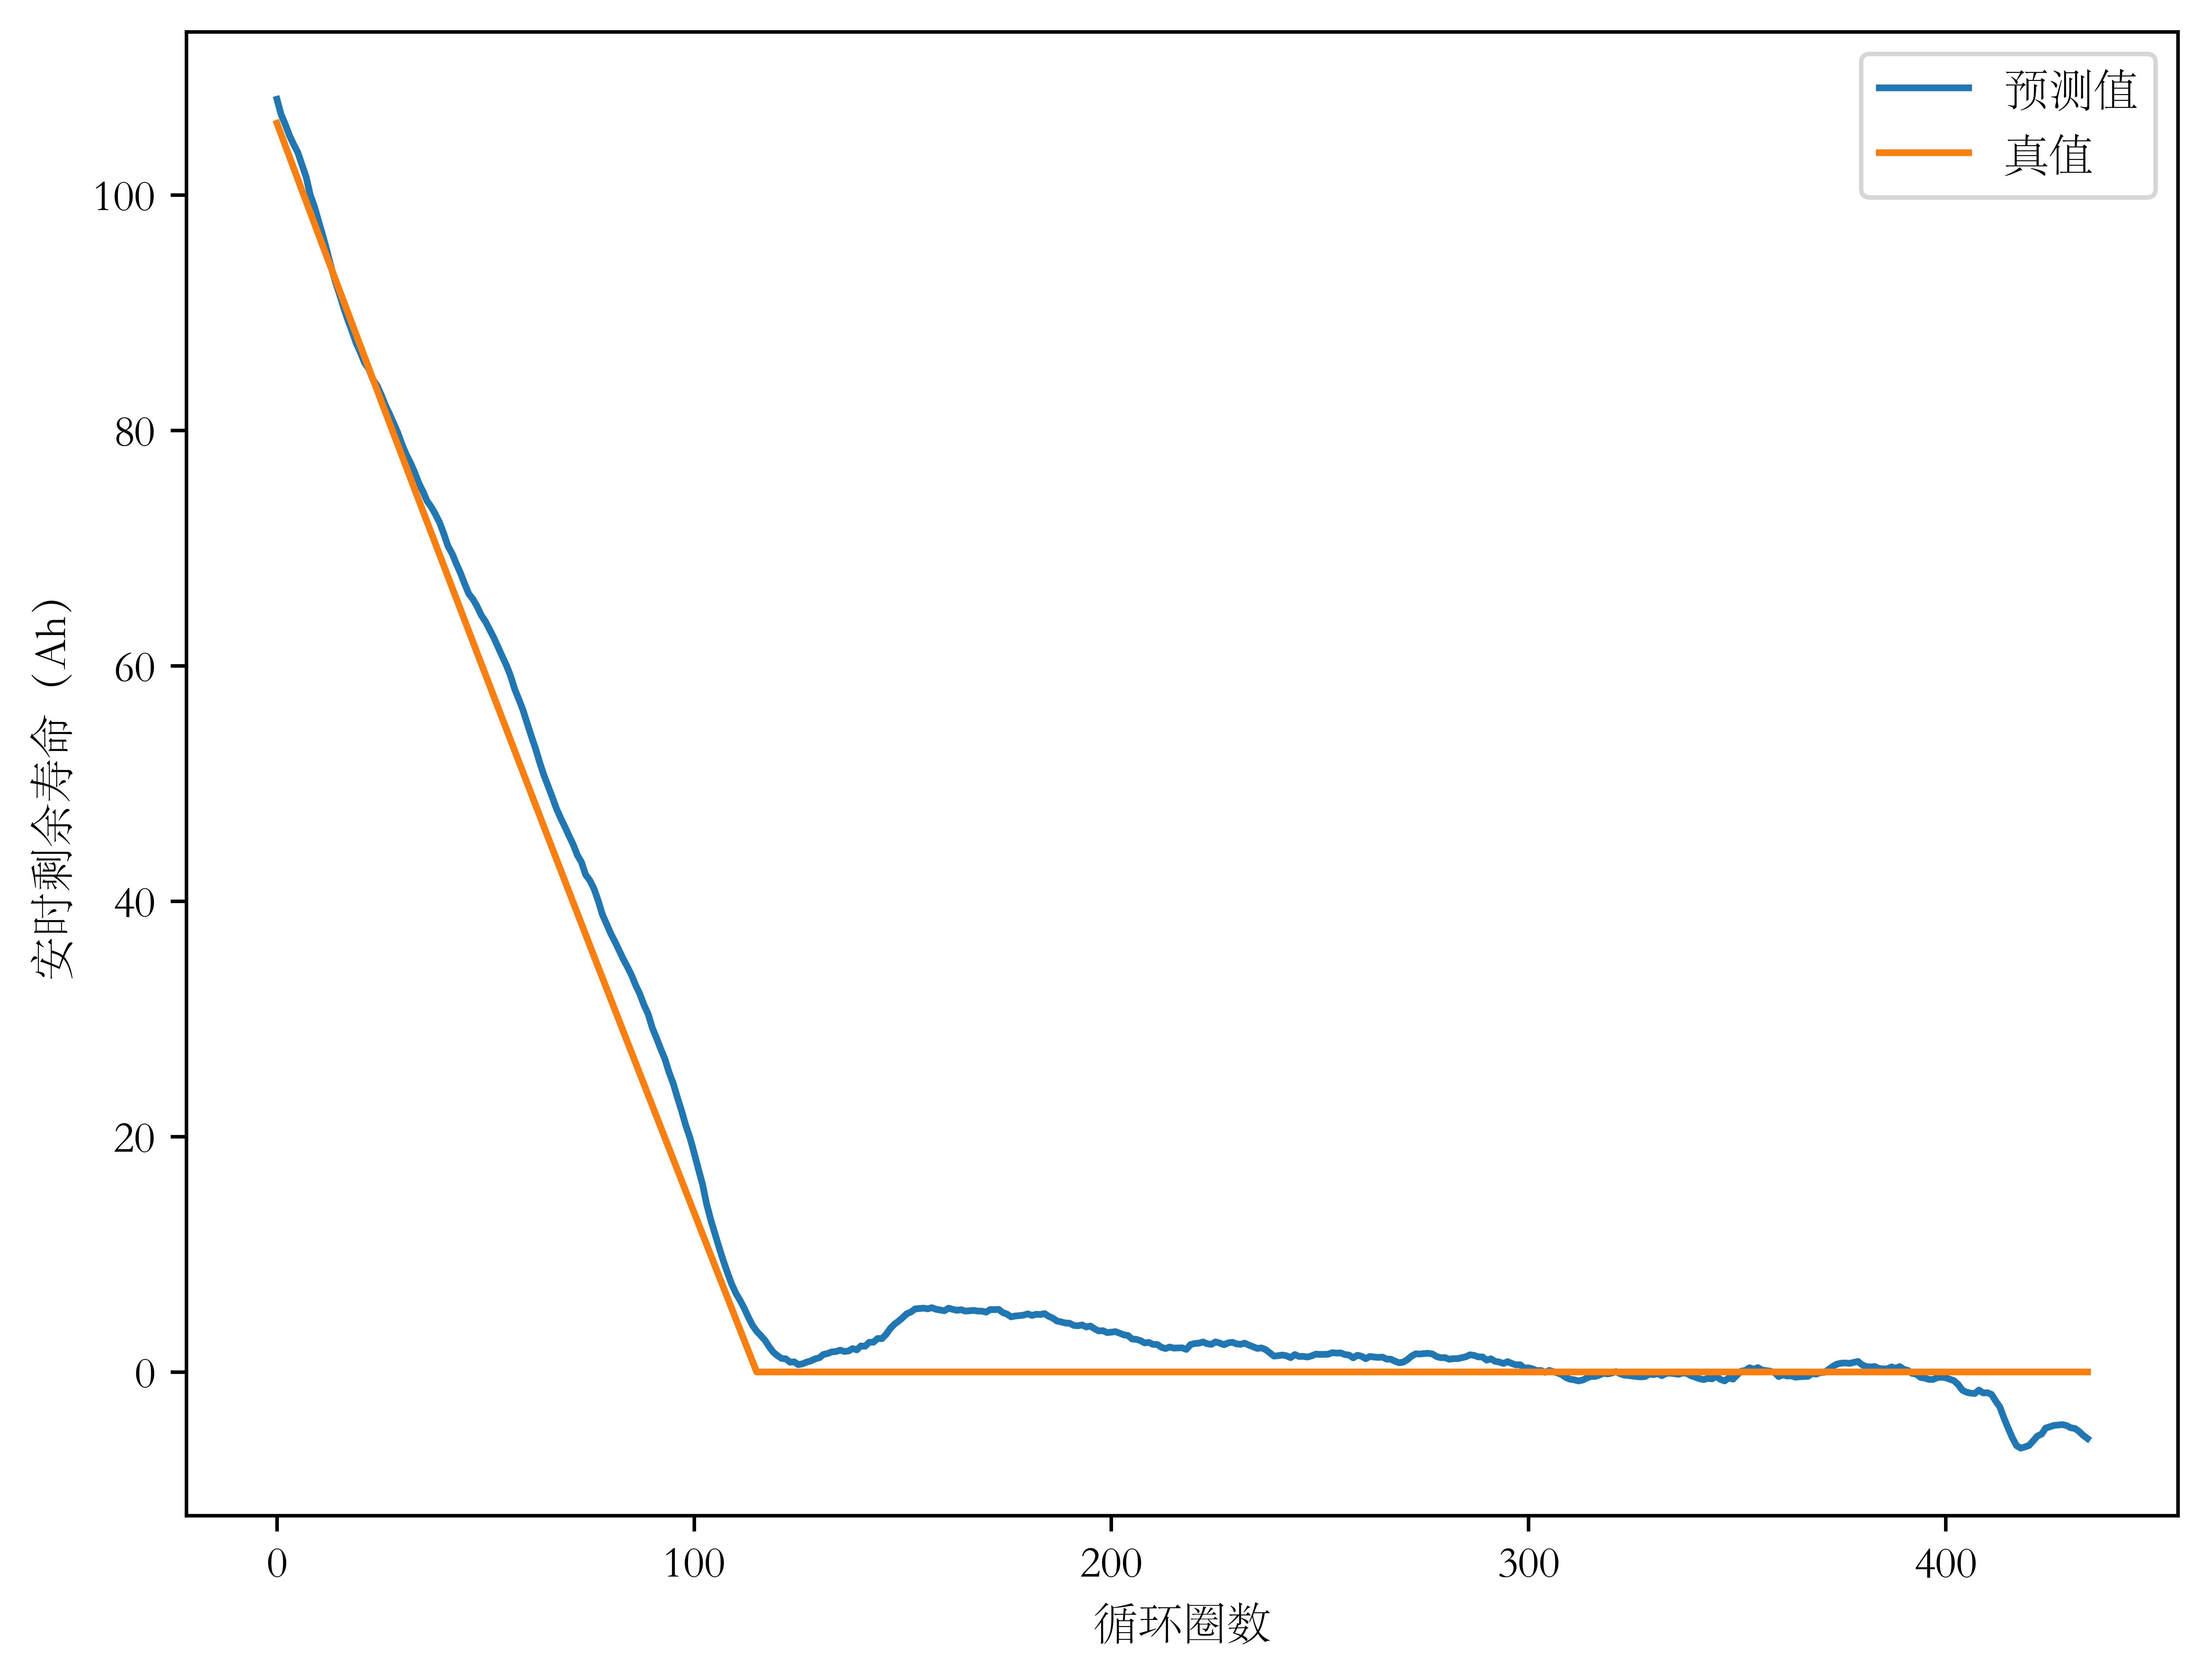
\includegraphics[width=0.3\textwidth]{figures/rul/unibo_lstm_rul_cycle_2.jpg}}
			{\label{fig:subfig2}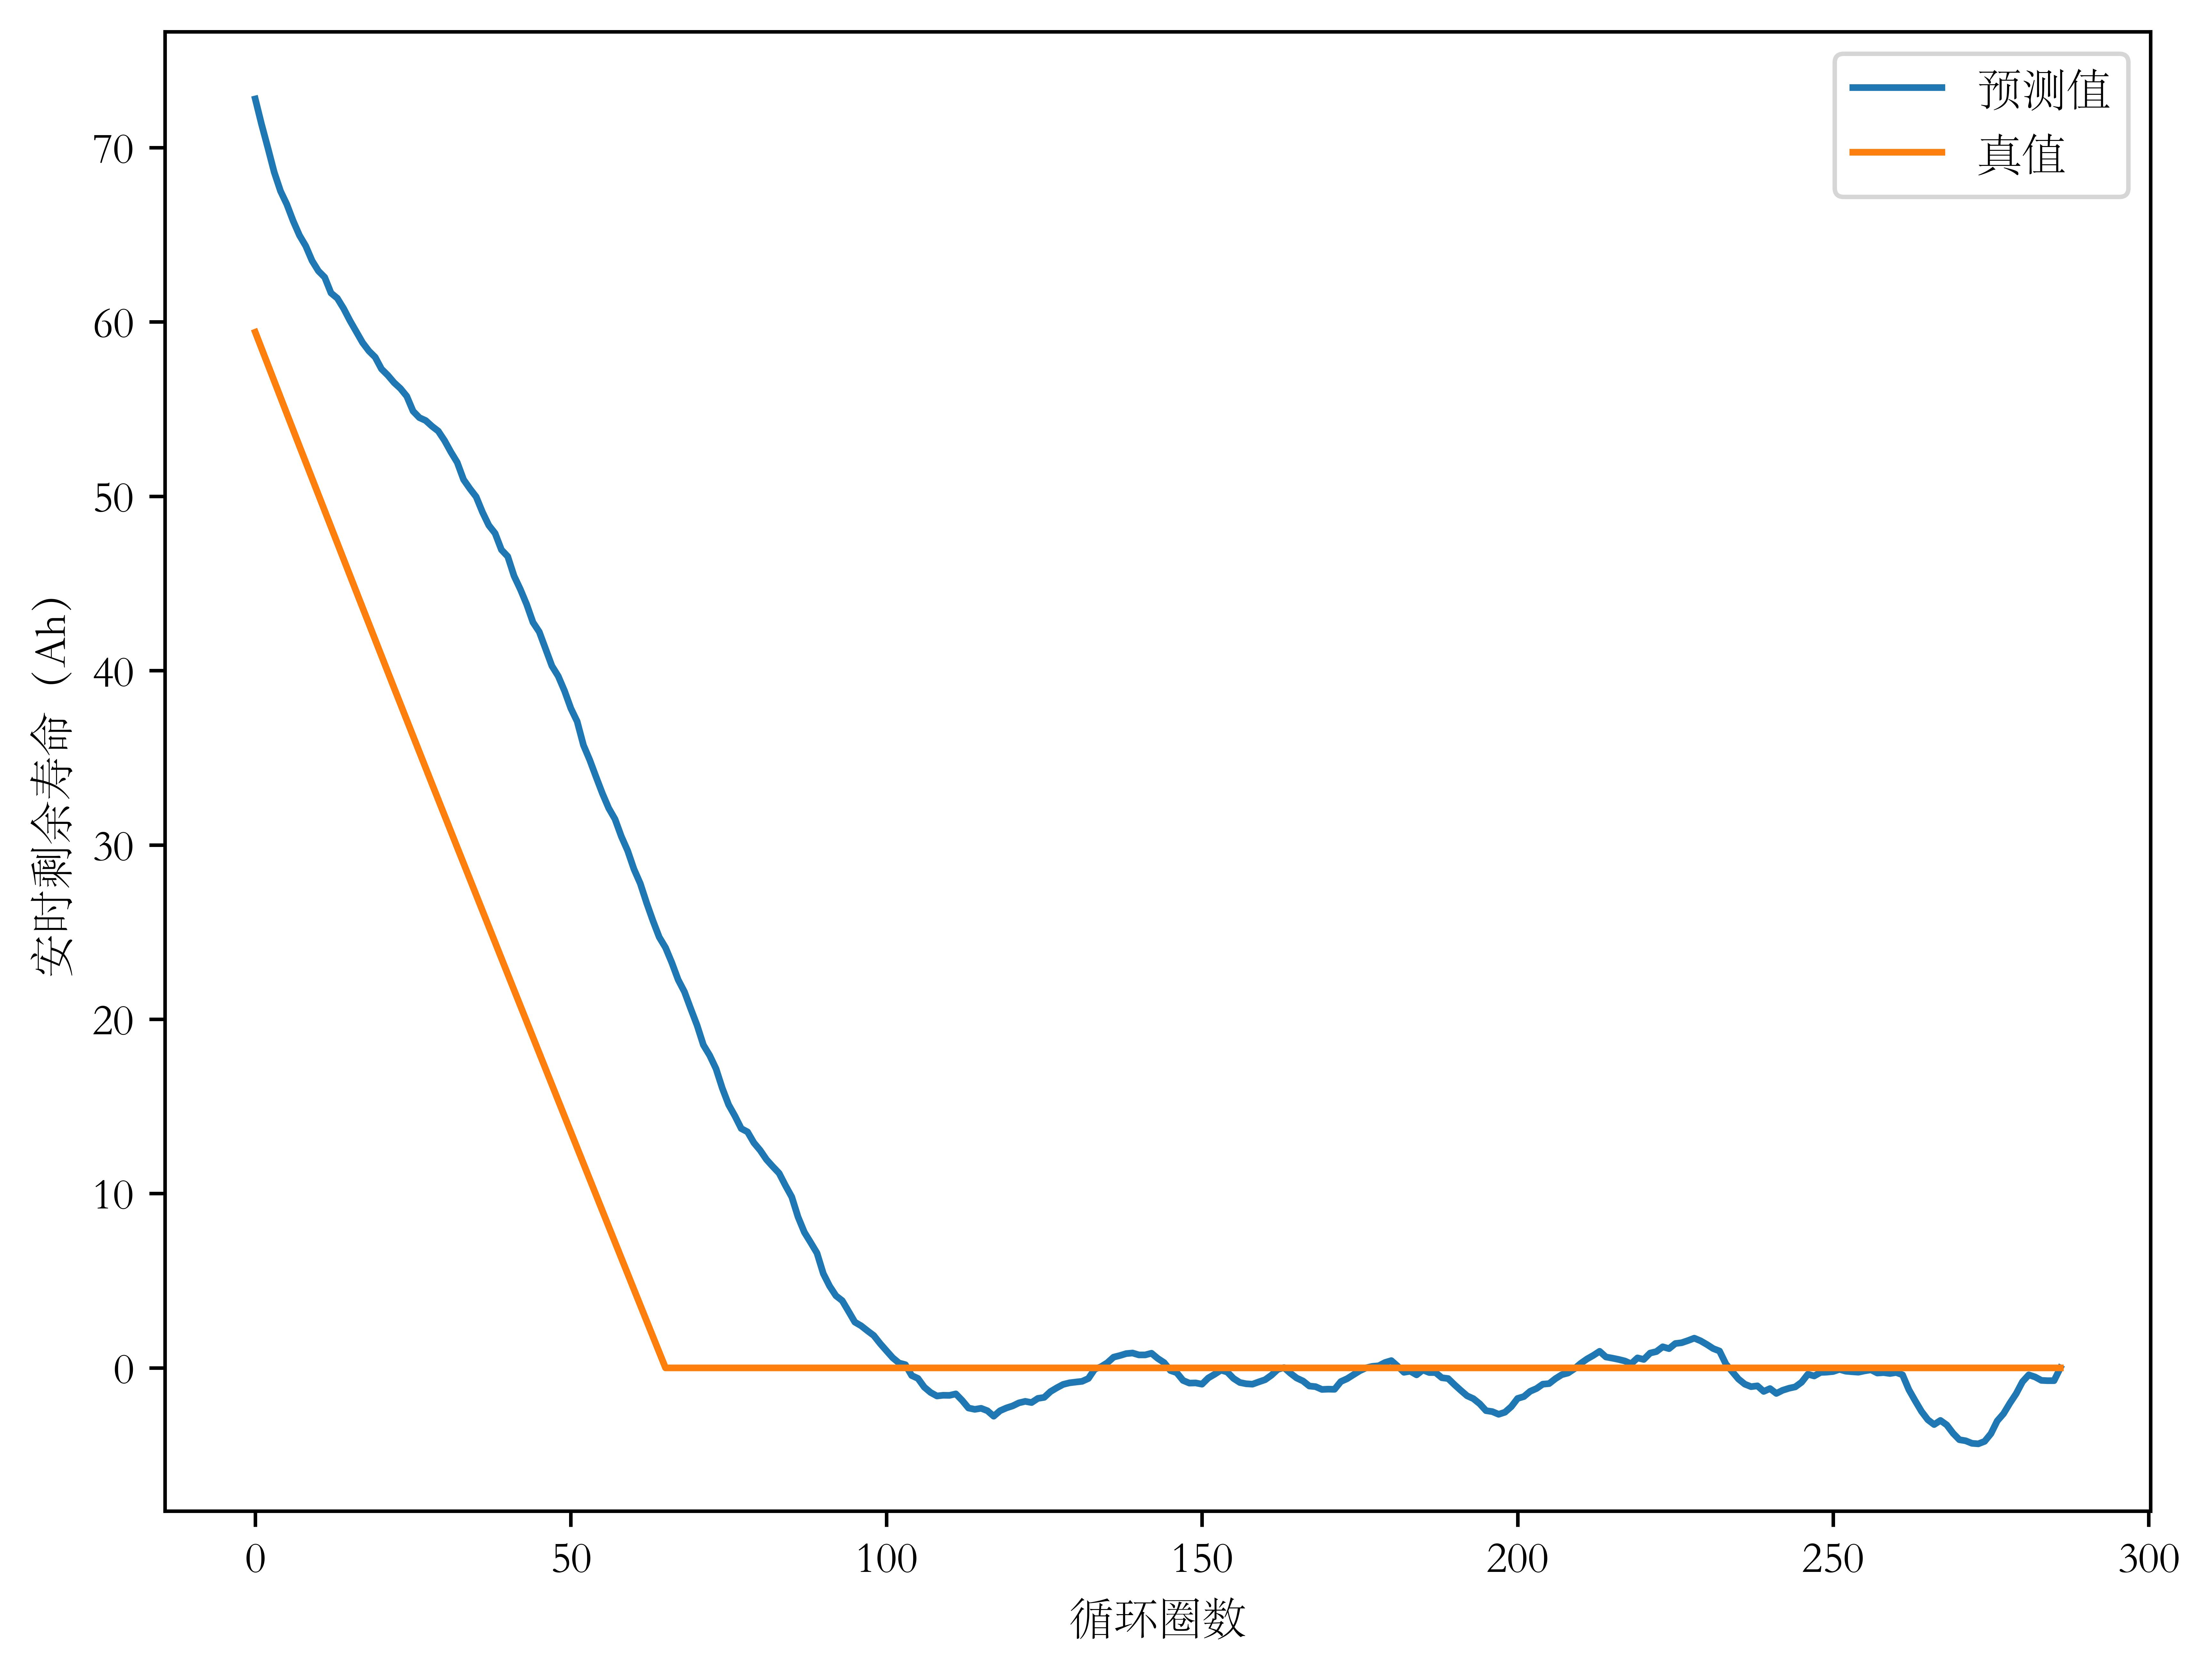
\includegraphics[width=0.3\textwidth]{figures/rul/unibo_lstm_rul_cycle_3.jpg}}
	\end{figure}
	\begin{figure}[htbp]
		\centering
			{\label{fig:subfig1}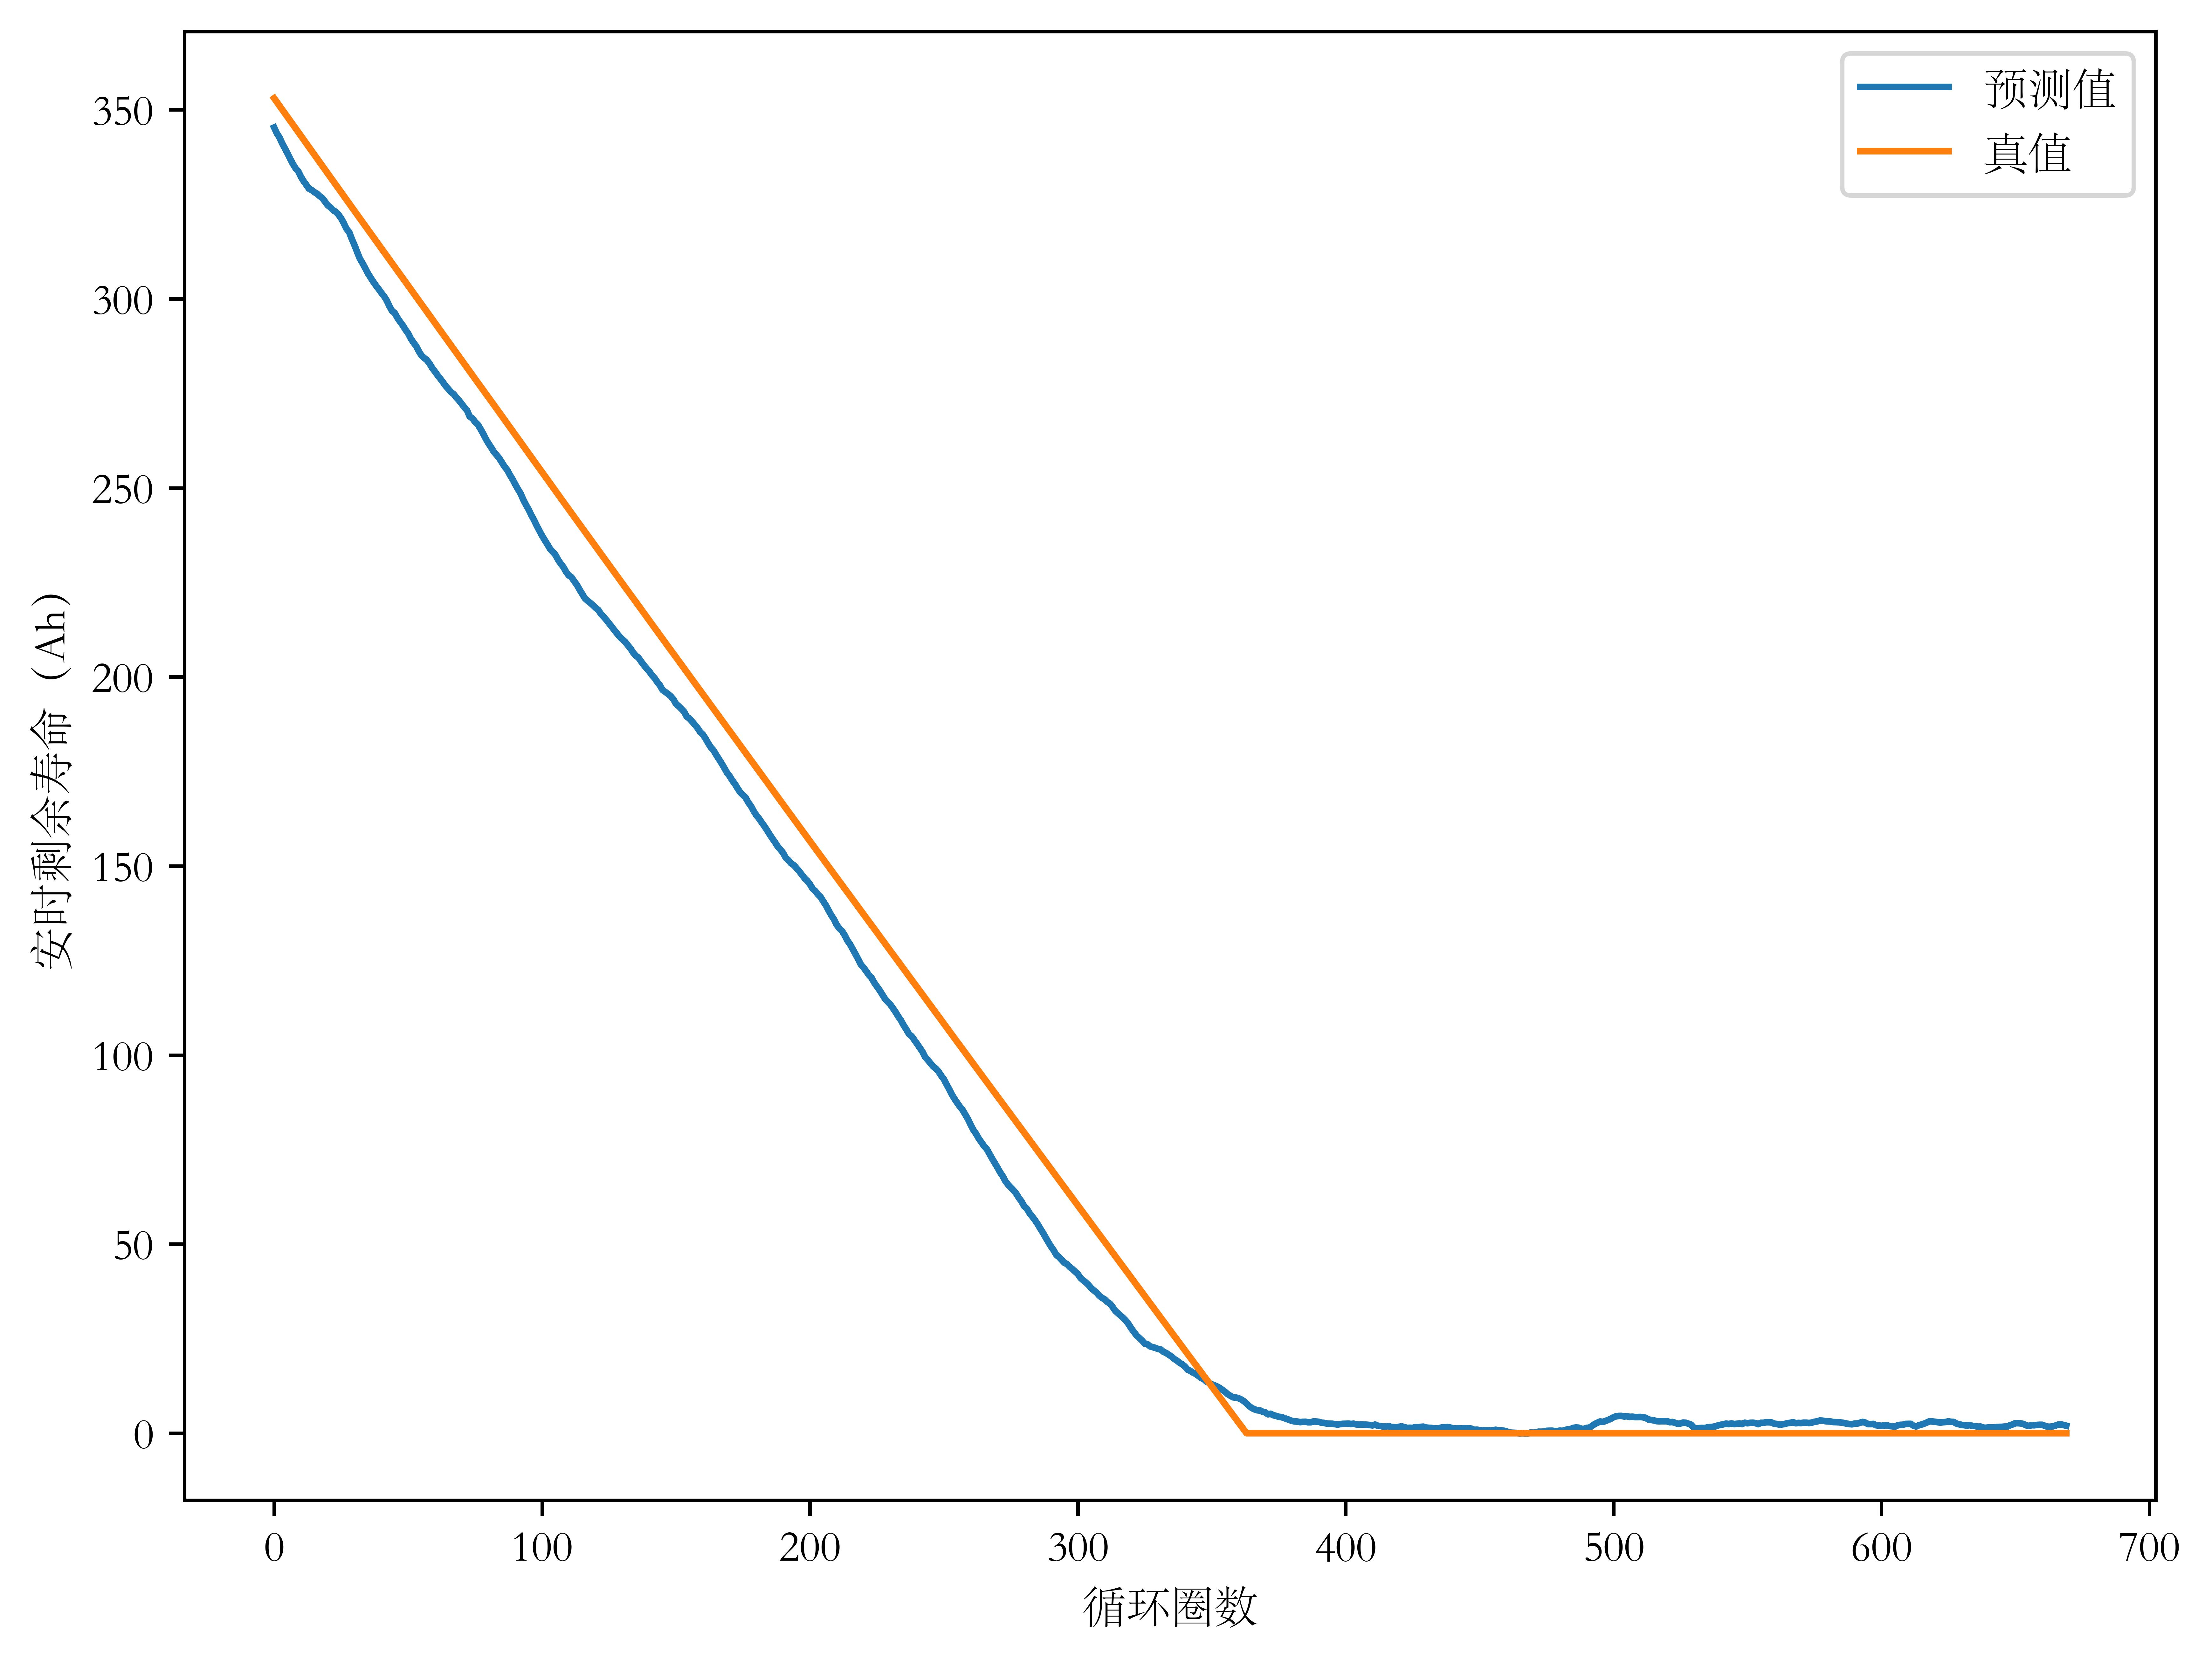
\includegraphics[width=0.3\textwidth]{figures/rul/unibo_lstm_rul_cycle_4.jpg}}
			{\label{fig:subfig2}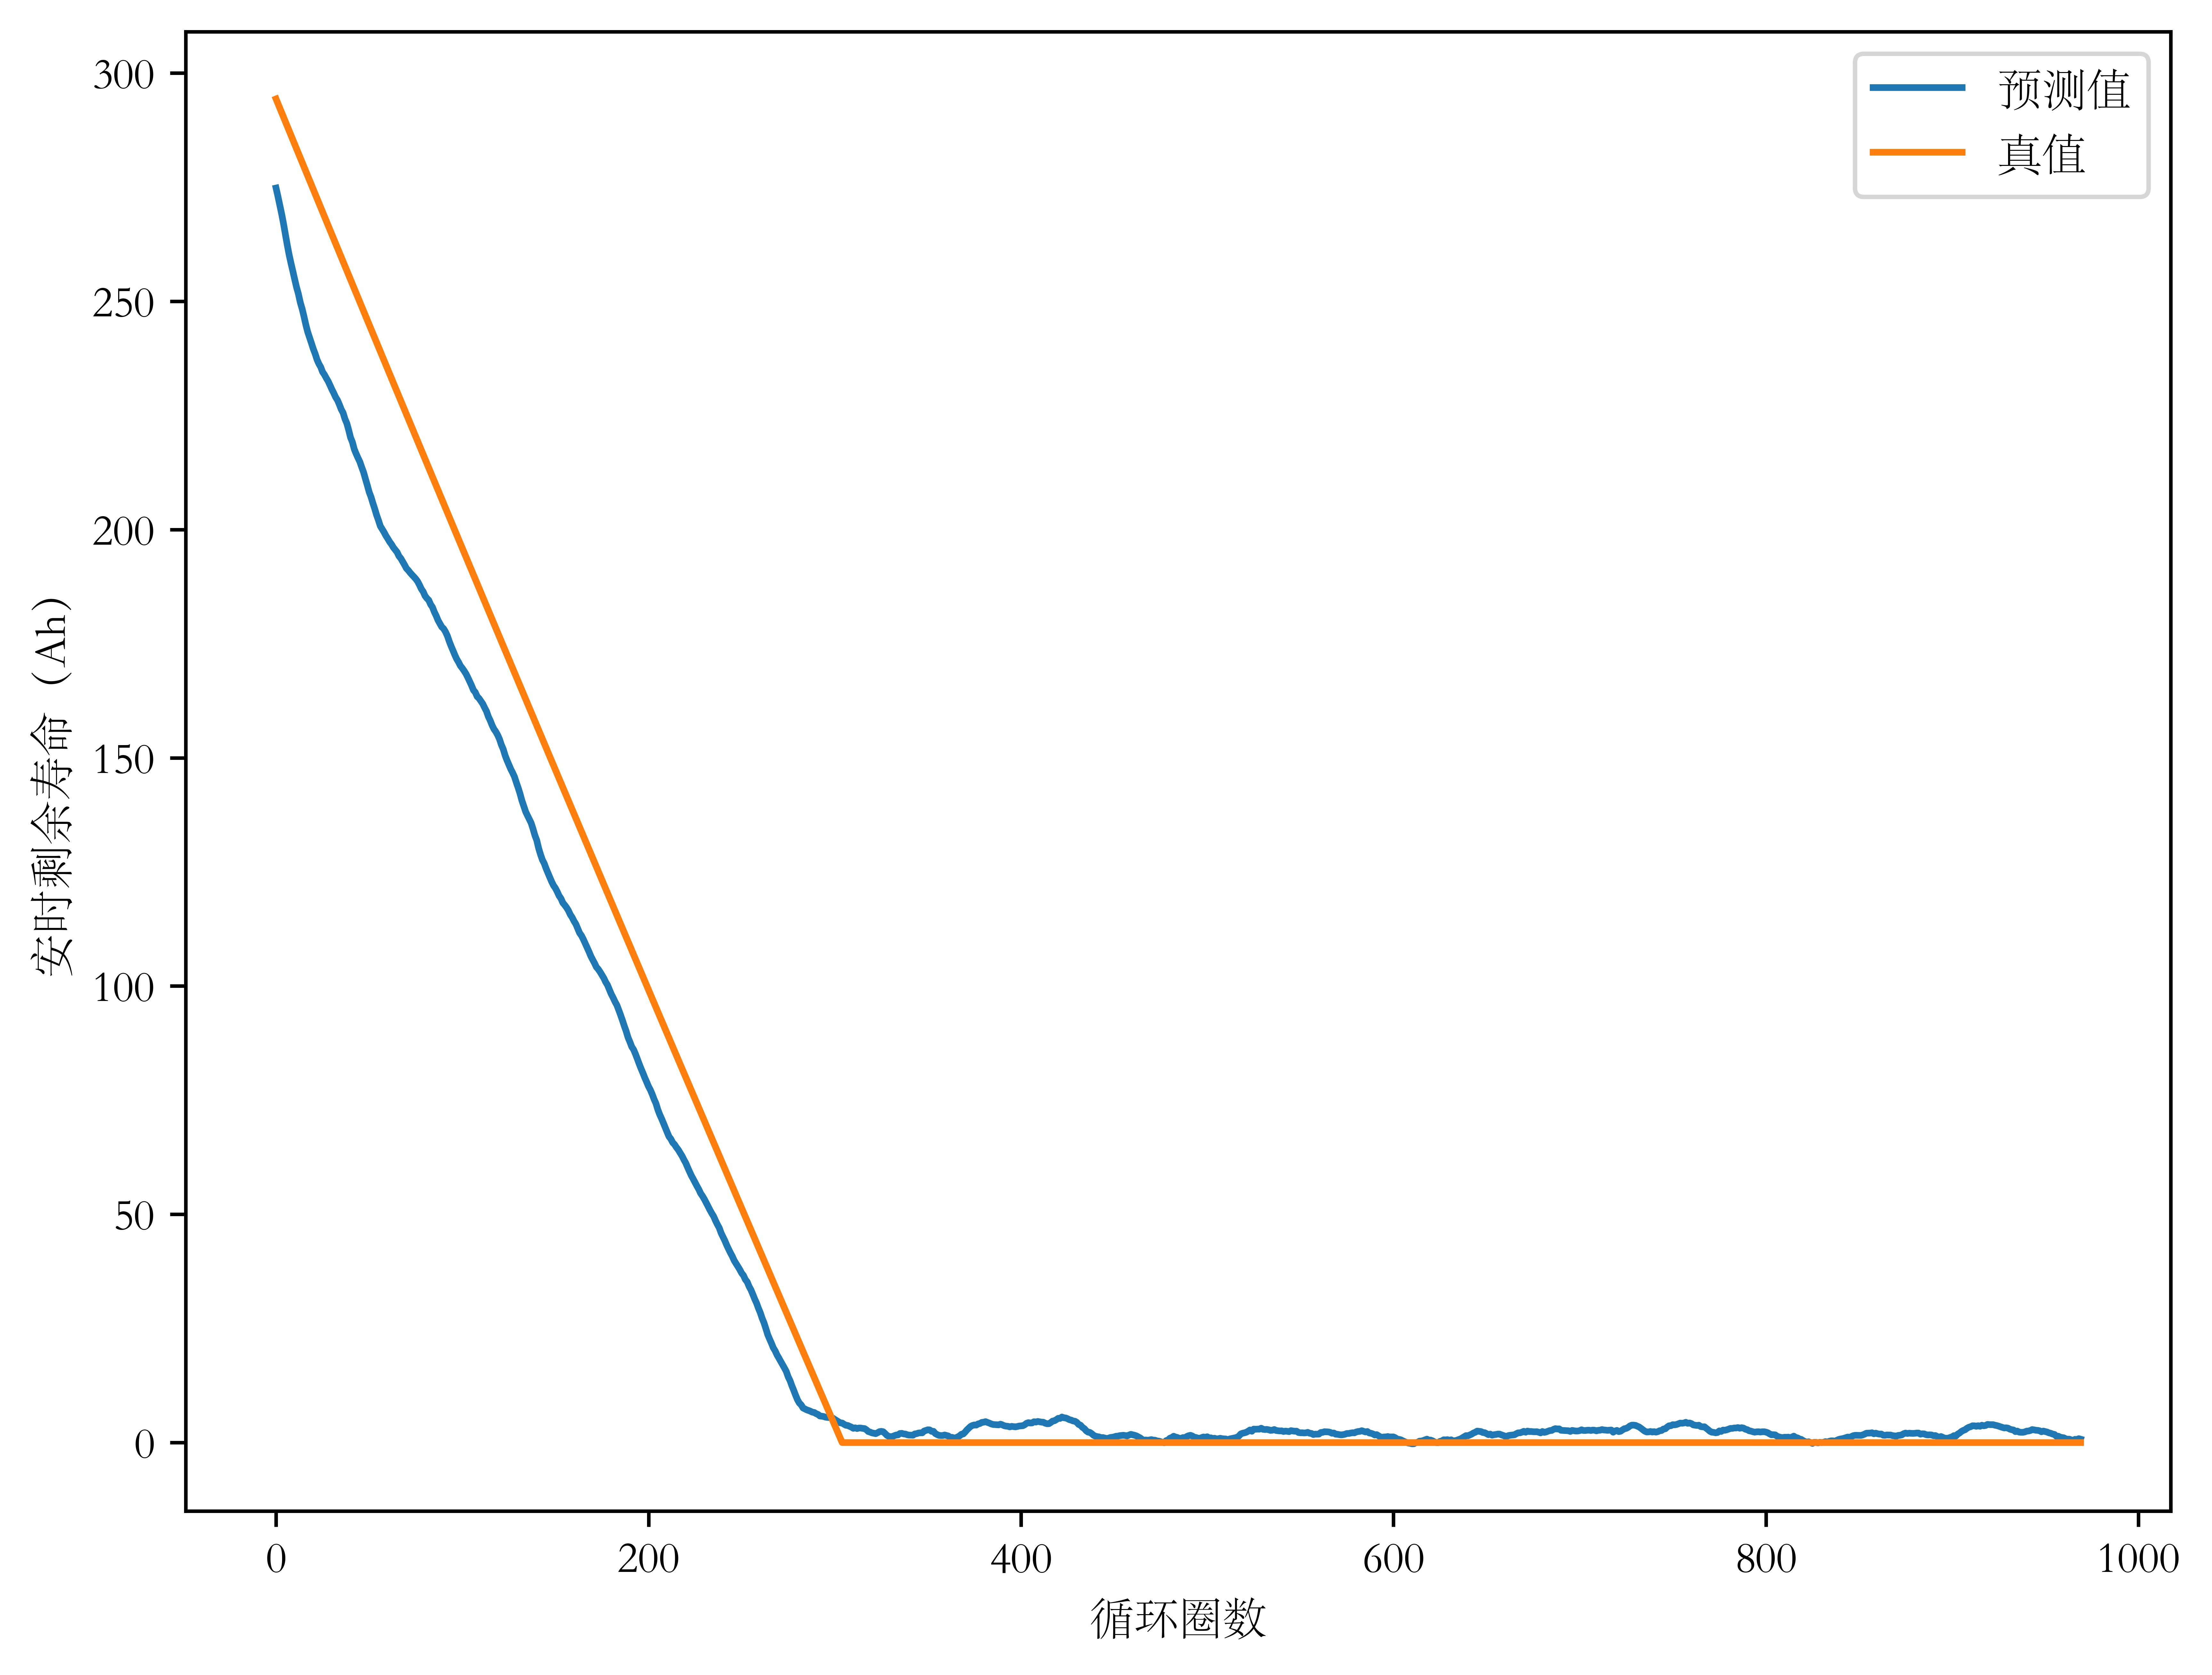
\includegraphics[width=0.3\textwidth]{figures/rul/unibo_lstm_rul_cycle_5.jpg}}
			{\label{fig:subfig2}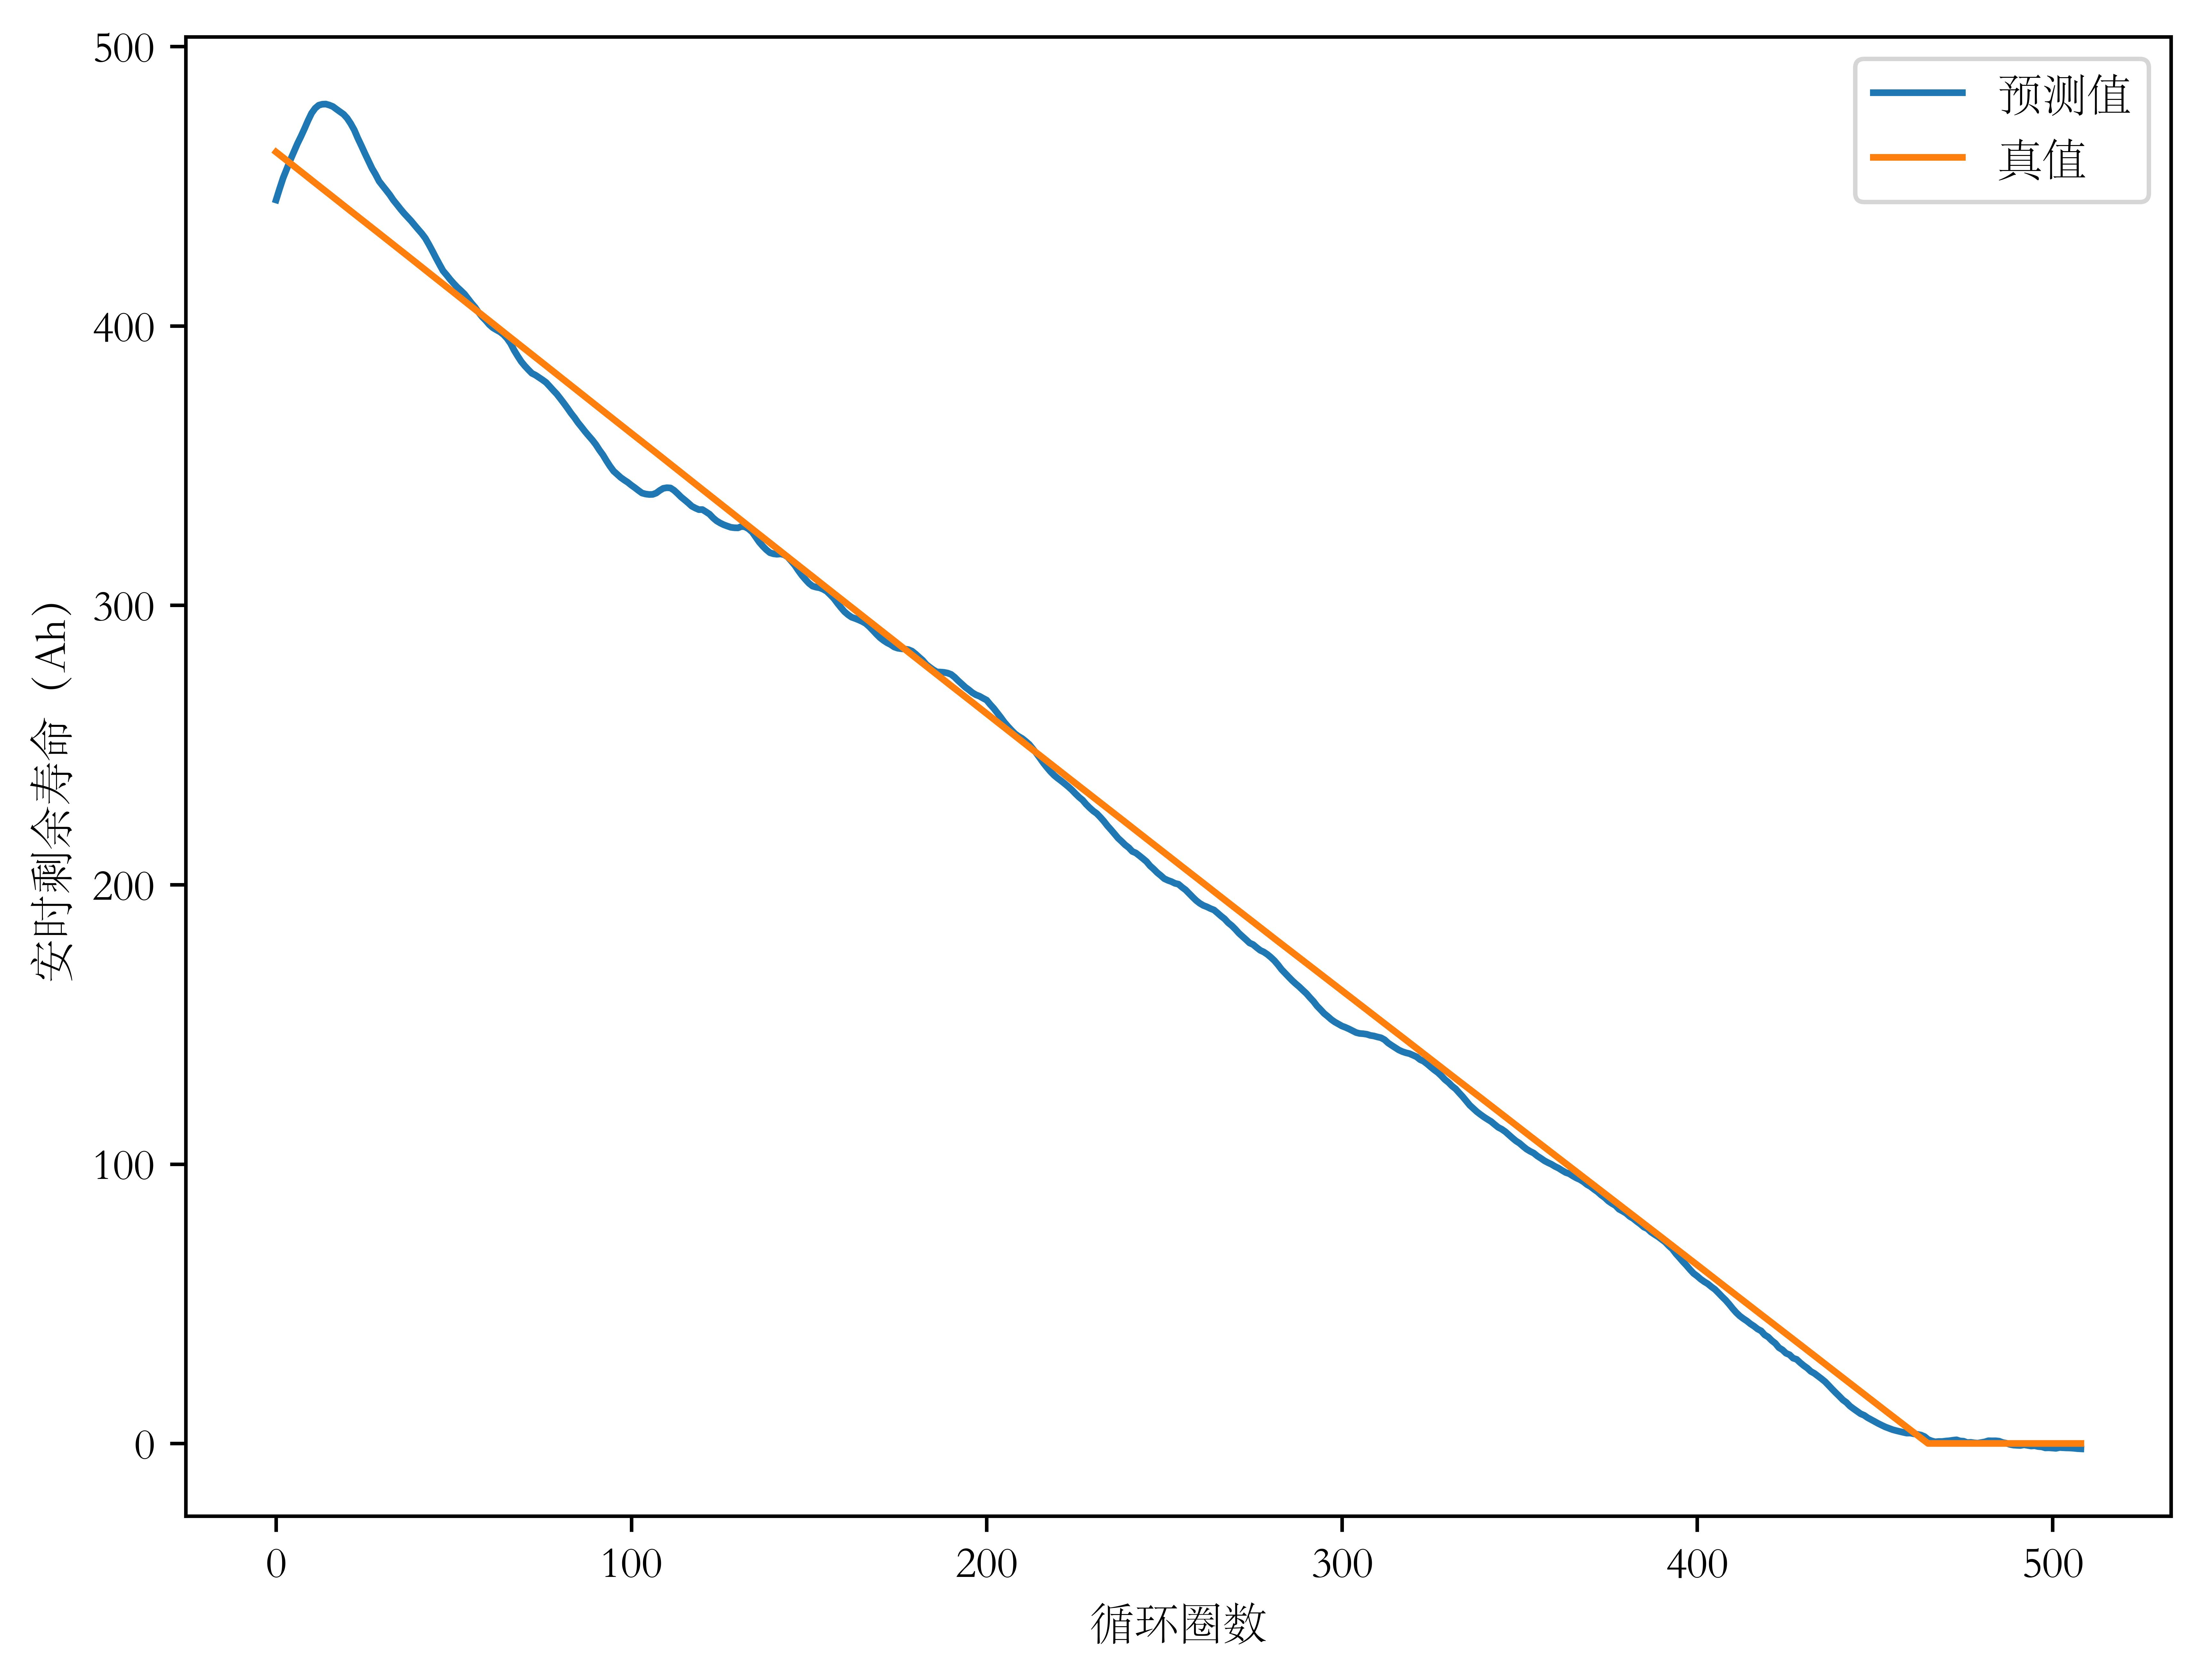
\includegraphics[width=0.3\textwidth]{figures/rul/unibo_lstm_rul_cycle_6.jpg}}
	\end{figure}
\end{frame}

\begin{frame}
	% Please add the following required packages to your document preamble:
% \usepackage{graphicx}
\begin{table}[]
	\centering
	\resizebox{\columnwidth}{!}{%
	\begin{tabular}{ccccccccc}
	\toprule
	指标    & 电池003    & 电池011    & 电池013    & 电池006    & 电池044    & 电池039    & 电池041    & 均值       \\
	\midrule
	RMSE  & 3.855191 & 3.102227 & 10.77393 & 10.12258 & 13.87137 & 8.883196 & 4.498271 & 7.872395 \\
	NRMSE & 0.035861 & 0.02924  & 0.181346 & 0.028673 & 0.047128 & 0.019219 & 0.051681 & 0.056164 \\  
	\bottomrule
	\end{tabular}%
	}
	\caption{\fontsize{10.5bp}{17bp}DeepLSTM模型电池Ah-RUL预测性能}
	\end{table}
	\begin{itemize}
		\item 实验结果表明使用数据驱动方法实现锂离子电池RUL预测具有可行性
	\end{itemize}
\end{frame}

\section{总结与展望}

\begin{frame}
	\begin{itemize}
		\item 总结
			\begin{itemize}
				\item 基于电池容量历史退化数据实现SOH估计,比较五种模型的预测性能
				\item 基于电池充放电直接测量量实现SOH估计,使用电荷量取代电池表明温度作为模型输入提高预测性能,使用时间序列-图像变换减少模型参数量
				\item 基于电池充放电直接测量量实现RUL预测,提出依据容量定义的Ah-RUL取代依据循环圈数定义的cycle-RUL
			\end{itemize}
		\item 展望
			\begin{itemize}
				\item 估计/预测模型改进
					\begin{itemize}
						\item 融合机理模型和数据驱动模型,提高模型性能
						\item 引入贝叶斯模型,实现对预测结果的不确定性度量以更好支持工业决策
						\item 引入迁移学习,提高模型泛化能力
					\end{itemize}
				\item 模型在嵌入式平台的部署:模型量化和模型转换
			\end{itemize}
	\end{itemize}
\end{frame}

\section{写在最后}

\begin{frame}
	\centering
	本课题相关代码已在github上开源,请见:

	\centering
	\url {https://github.com/hilinxinhui/battery_phm.git}

	\begin{figure}[htbp]
		\centering
		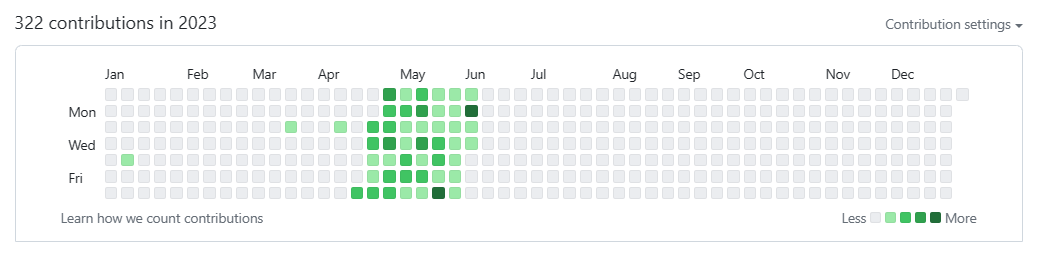
\includegraphics[scale=0.35]{figures/github_contribution_log.png}
	\end{figure}

	\begin{figure}[htbp]
		\centering
		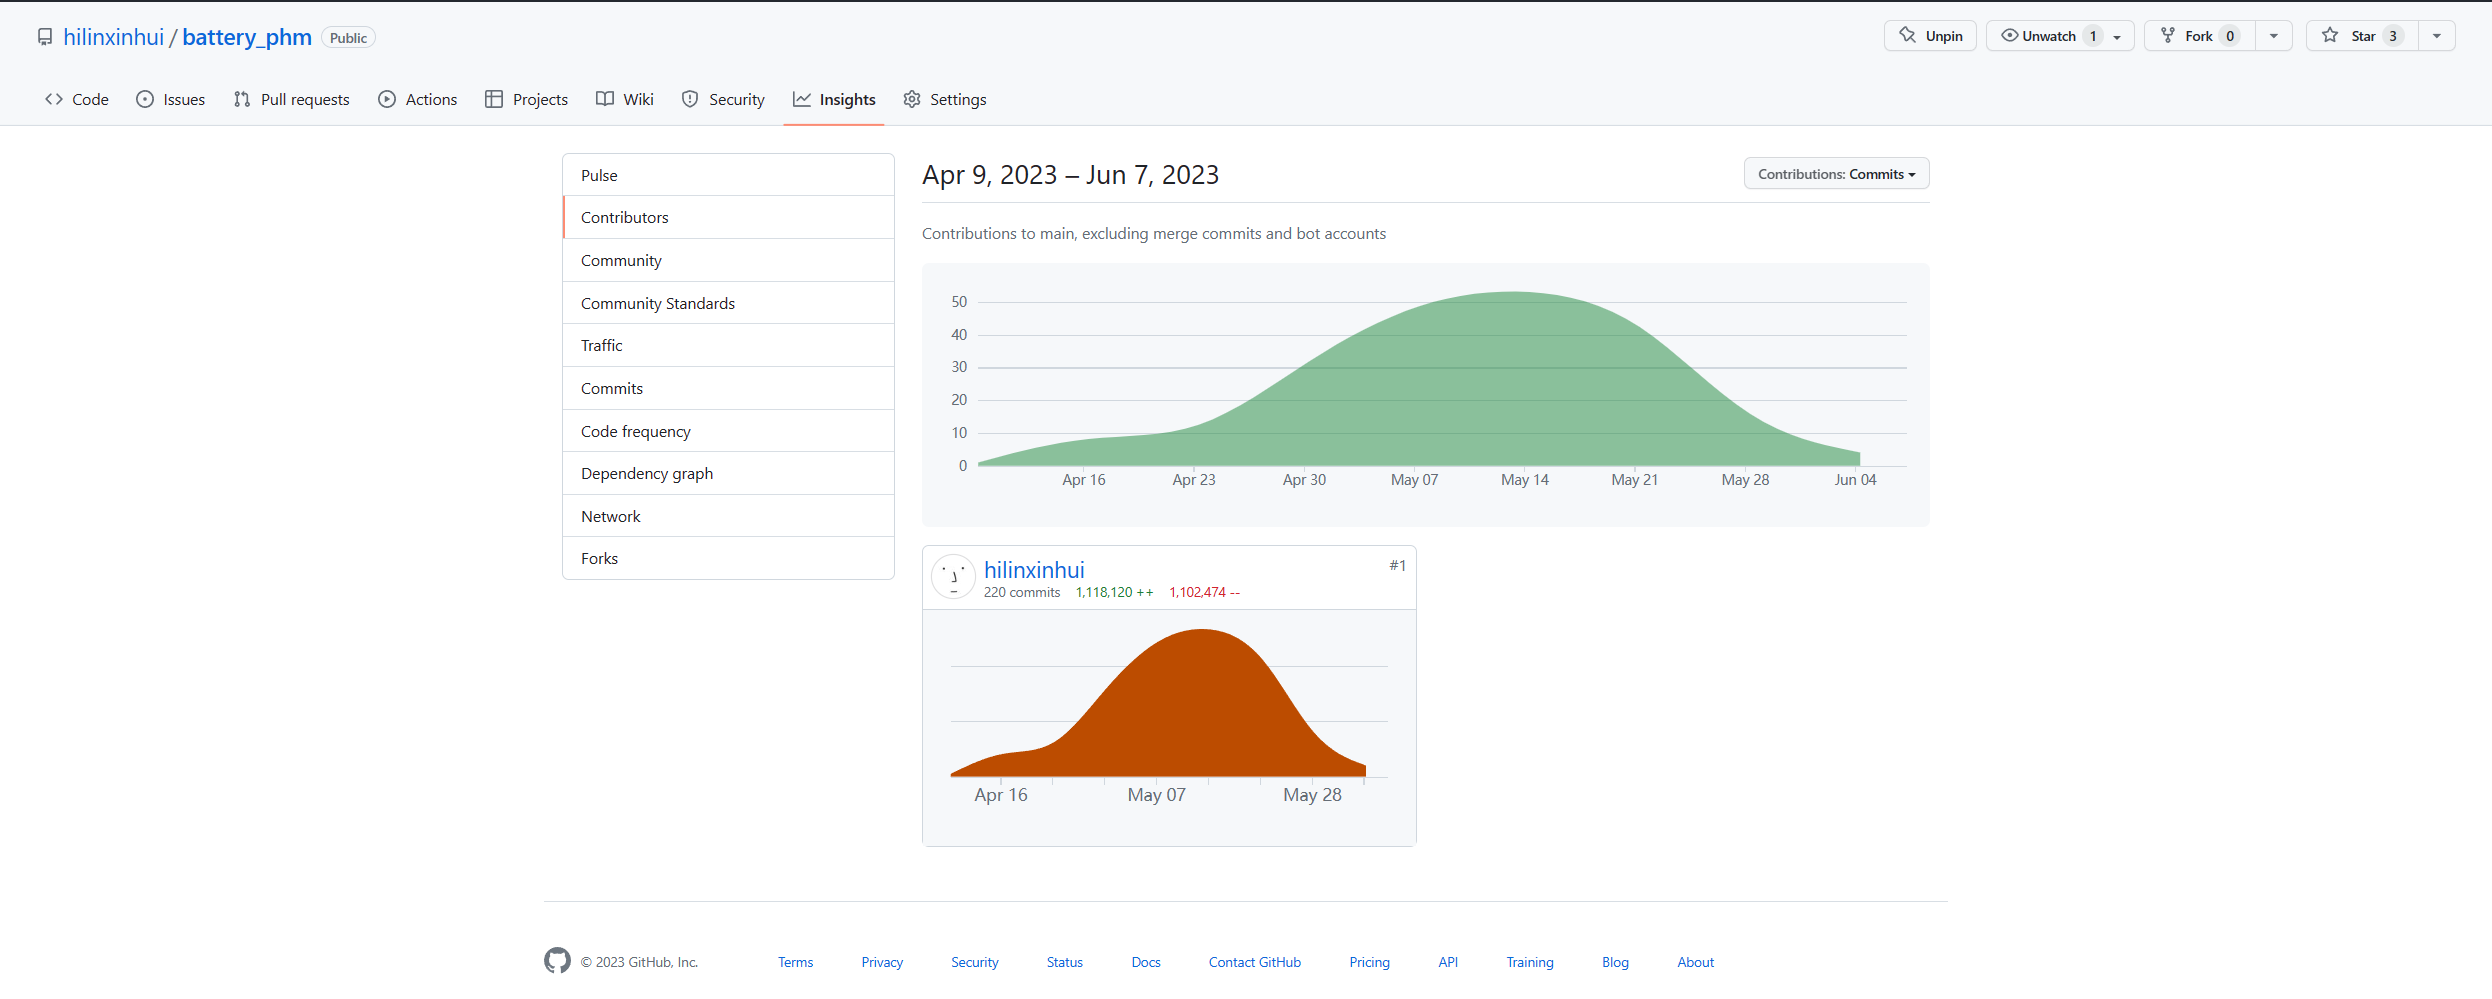
\includegraphics[scale=0.15]{figures/github_contribution_log_2.png}
	\end{figure}

\end{frame}

\begin{frame}{感谢各位老师}
	\LARGE \centering 汇报完毕,请各位老师批评指正!
\end{frame}

\end{document}
